\documentclass[twoside]{book}

% Packages required by doxygen
\usepackage{fixltx2e}
\usepackage{calc}
\usepackage{doxygen}
\usepackage[export]{adjustbox} % also loads graphicx
\usepackage{graphicx}
\usepackage[utf8]{inputenc}
\usepackage{makeidx}
\usepackage{multicol}
\usepackage{multirow}
\PassOptionsToPackage{warn}{textcomp}
\usepackage{textcomp}
\usepackage[nointegrals]{wasysym}
\usepackage[table]{xcolor}

% Font selection
\usepackage[T1]{fontenc}
\usepackage[scaled=.90]{helvet}
\usepackage{courier}
\usepackage{amssymb}
\usepackage{sectsty}
\renewcommand{\familydefault}{\sfdefault}
\allsectionsfont{%
  \fontseries{bc}\selectfont%
  \color{darkgray}%
}
\renewcommand{\DoxyLabelFont}{%
  \fontseries{bc}\selectfont%
  \color{darkgray}%
}
\newcommand{\+}{\discretionary{\mbox{\scriptsize$\hookleftarrow$}}{}{}}

% Page & text layout
\usepackage{geometry}
\geometry{%
  a4paper,%
  top=2.5cm,%
  bottom=2.5cm,%
  left=2.5cm,%
  right=2.5cm%
}
\tolerance=750
\hfuzz=15pt
\hbadness=750
\setlength{\emergencystretch}{15pt}
\setlength{\parindent}{0cm}
\setlength{\parskip}{3ex plus 2ex minus 2ex}
\makeatletter
\renewcommand{\paragraph}{%
  \@startsection{paragraph}{4}{0ex}{-1.0ex}{1.0ex}{%
    \normalfont\normalsize\bfseries\SS@parafont%
  }%
}
\renewcommand{\subparagraph}{%
  \@startsection{subparagraph}{5}{0ex}{-1.0ex}{1.0ex}{%
    \normalfont\normalsize\bfseries\SS@subparafont%
  }%
}
\makeatother

% Headers & footers
\usepackage{fancyhdr}
\pagestyle{fancyplain}
\fancyhead[LE]{\fancyplain{}{\bfseries\thepage}}
\fancyhead[CE]{\fancyplain{}{}}
\fancyhead[RE]{\fancyplain{}{\bfseries\leftmark}}
\fancyhead[LO]{\fancyplain{}{\bfseries\rightmark}}
\fancyhead[CO]{\fancyplain{}{}}
\fancyhead[RO]{\fancyplain{}{\bfseries\thepage}}
\fancyfoot[LE]{\fancyplain{}{}}
\fancyfoot[CE]{\fancyplain{}{}}
\fancyfoot[RE]{\fancyplain{}{\bfseries\scriptsize Generated by Doxygen }}
\fancyfoot[LO]{\fancyplain{}{\bfseries\scriptsize Generated by Doxygen }}
\fancyfoot[CO]{\fancyplain{}{}}
\fancyfoot[RO]{\fancyplain{}{}}
\renewcommand{\footrulewidth}{0.4pt}
\renewcommand{\chaptermark}[1]{%
  \markboth{#1}{}%
}
\renewcommand{\sectionmark}[1]{%
  \markright{\thesection\ #1}%
}

% Indices & bibliography
\usepackage{natbib}
\usepackage[titles]{tocloft}
\setcounter{tocdepth}{3}
\setcounter{secnumdepth}{5}
\makeindex

% Hyperlinks (required, but should be loaded last)
\usepackage{ifpdf}
\ifpdf
  \usepackage[pdftex,pagebackref=true]{hyperref}
\else
  \usepackage[ps2pdf,pagebackref=true]{hyperref}
\fi
\hypersetup{%
  colorlinks=true,%
  linkcolor=blue,%
  citecolor=blue,%
  unicode%
}

% Custom commands
\newcommand{\clearemptydoublepage}{%
  \newpage{\pagestyle{empty}\cleardoublepage}%
}

\usepackage{caption}
\captionsetup{labelsep=space,justification=centering,font={bf},singlelinecheck=off,skip=4pt,position=top}

%===== C O N T E N T S =====

\begin{document}

% Titlepage & ToC
\hypersetup{pageanchor=false,
             bookmarksnumbered=true,
             pdfencoding=unicode
            }
\pagenumbering{alph}
\begin{titlepage}
\vspace*{7cm}
\begin{center}%
{\Large C\+S\+CI 3081 -\/ Drone Delivery System }\\
\vspace*{1cm}
{\large Generated by Doxygen 1.8.13}\\
\end{center}
\end{titlepage}
\clearemptydoublepage
\pagenumbering{roman}
\tableofcontents
\clearemptydoublepage
\pagenumbering{arabic}
\hypersetup{pageanchor=true}

%--- Begin generated contents ---
\chapter{C\+S\+CI 3081 Delivery Simulation project}
\label{index}\hypertarget{index}{}{\bfseries Iteration 3 J\+S\+ON File} We would like you to test our Iteration 3 Deliverable on the all\+\_\+features.\+json file that we have altered in our scenes folder. This should provide a simulation in which drones and robots are continuously recharged as they run out of battery during their deliveries ~\newline


{\bfseries Extra Credit} This version does run on the extra credit files, including\+: multiple\+\_\+drones.\+json, multiple\+\_\+customers.\+json, multiple\+\_\+packages.\+json, and multiple\+\_\+deliveries.\+json ~\newline


{\bfseries To obtain the code}, in the terminal, type\+: 
\begin{DoxyPre} \$ git clone \href{https://github.umn.edu/umn-csci-3081-s21/repo-iter2-10-22.git}{\tt https://github.umn.edu/umn-csci-3081-s21/repo-iter2-10-22.git} \end{DoxyPre}
 This will prompt you to sign in into your Github. If you have the right access, you would be able to obtain the code. To compile the code, navigate to the \char`\"{}repo-\/iter2-\/10-\/22\char`\"{} directory that you just download from github by typing\+: 
\begin{DoxyPre} \$ cd repo-iter2-10-22 \end{DoxyPre}
 To compile the code$\ast$$\ast$, in the terminal, type\+: 
\begin{DoxyPre} \$ make \end{DoxyPre}
 {\bfseries To run the simulation}, there are two ways\+:
\begin{DoxyItemize}
\item If you are using {\bfseries Docker}, after install all of the Docker software needed for your environment, in directory \char`\"{}repo-\/iter2-\/10-\/22\char`\"{}, type the following commands to the terminal\+: 
\begin{DoxyPre} \$ bin/build-env.sh \end{DoxyPre}
 This will help build the docker image. To run docker image\+: 
\begin{DoxyPre} bin/run-env.sh \end{DoxyPre}
 Build project web server (inside docker image), navigate to the \char`\"{}repo-\/iter2-\/10-\/22\char`\"{} directory, then\+: 
\begin{DoxyPre} \$ make \end{DoxyPre}
 To run the web server (inside docker image), inside \char`\"{}repo-\/iter2-\/10-\/22\char`\"{} directory\+: 
\begin{DoxyPre} \$ ./bin/run.sh \end{DoxyPre}

\item If you are using {\bfseries V\+O\+LE}, navigate to \char`\"{}repo-\/iter2-\/10-\/22\char`\"{} directory, then 
\begin{DoxyPre} \$ cd project \end{DoxyPre}
 
\begin{DoxyPre} \$ make \end{DoxyPre}
 
\begin{DoxyPre} \$ ./bin/run.sh \end{DoxyPre}

\item Note that the project is not designed to work on S\+SH yet ~\newline
 {\bfseries Dicussion of concrete factory pattern vs. abstract factory pattern vs. composite factory pattern}
\end{DoxyItemize}

\begin{center}  \end{center} 

First, we begin with the concrete factory pattern. As we can see in Figure 1, there is a new class call Entity\+Factory that is responsible for creating Entity. This prevents the program to have a lot of different Entity derived classes and to not know which one would be created until runtime. This is good; however, there is still tight coupling. Everytime we have a new Entity derived class, we have to add new case/ new if else statement in Entity\+Factory. Here is how Abstract Factory come to the story.

\begin{center}  \end{center} 

Figure 2 depicts how the U\+ML of this program would look like if we employ Abstract Factory pattern. Entity\+Factory becomes an abstract class, pushing the creation of each Entity derived class into subclasses. For example, Drone object is created by Drone\+Factory. With this model, every time we create a new Entity derived class, we just need to create a new subclass of Entity\+Factory. However, even with this pattern, the Create\+Entity function of Delivery\+Simulation still contains a thread of if-\/else statement to decide which Entity to create. This is not idea, since every time we add a new Entity derived class, we still have to edit our Create\+Entity function in Delivery\+Simulation. This is where Composite Factory Pattern helps.

\begin{center} \end{center} 

With the Composite Factory pattern, we can just create a Composite\+Factory attribute in Deliver\+Simulation class, then use that to link to the other attribute. This would eliminate the long list of if and else statement anywhere in the code, and allow easy addition of new Entity derived as well as Entity\+Factory derived classes.

{\bfseries Discussion about the composite factory pattern} implemented in the package delivery system\+:

So we have discussed about the advantage of Composite Factory Pattern in the previous section. This pattern is excellent; however, it does have some disadvantages. The most obvious cons of composite factory pattern is that it might be difficult to provide a common interface for classes whose functionality differs too much. We might need to overgeneralize the componenent interface, making it harder to comprehend. In addition, the cons from this package delivery simulation, the composite factory pattern requires more classes to be created. It is hard to see the relationship between these classes even with a U\+ML diagram.

{\bfseries Designing and Implementing Strategy Pattern} ~\newline


In order to implement the strategy pattern in regards to choosing which route strategy for the drone to follow, we had to make several changes to our existing code. First, we had to create the interface which the concrete strategies would override. This abstract interface class is called Route\+Strategy and it has the method Get\+Route. We also have three concrete strategy classes; Smart\+Route, Beeline\+Route, and Parabolic\+Route. These concrete classes inherit from Route\+Strategy, and they implement the Get\+Route method to their own specifications. Once we had this structure in place, we had to alter the drone and robot classes to extract the path type information from the json details. Once the constructor was aware of which type of path was specified, it would store a pointer to that class type in it’s route\+Strategy attribute. This way, when we are in the delivery simulation, we can call the Get\+Route method from the route\+Strategy attribute of the carrier. The default route is set to smart path, and for the robots, only smart path is implemented (as robots cannot fly).

\begin{center}  Beeline\+Route, Smart\+Route and Parabolic\+Route" \end{center} 

At first it was difficult to understand the strategy pattern for us, but after working through different examples in class and online (\href{https://www.geeksforgeeks.org/strategy-pattern-set-2/}{\tt https\+://www.\+geeksforgeeks.\+org/strategy-\/pattern-\/set-\/2/}), we were able to better apply the strategy pattern to our own code.

{\bfseries Designing and Implementing Observer Pattern} ~\newline


In this project, {\bfseries observer Pattern} is implemented to notify the observers (the Web\+Scene\+Viewers and the Entity\+Console\+Logger) about change(s) in subjects (drones, robots, or packages). For the drones and robots, notifications are sent when they become idle or moving. For the packages, notifications are sent when the package is scheduled to be delivered, is en route (picked up), or is delivered.

We are given the implementation of the Observer classes (including the Web\+Scene\+Viewers and the Entity\+Console\+Logger classes), and therefore only need to write implementations for A\+Subject class, as well as its functionaility, and relate it to Drone, Package and Robot class. Following is the U\+ML depecting the relationship of the Observer pattern that we implement.

\begin{center}  and package to selected observers" \end{center} 

{\bfseries Designing and Implementing Different Route} ~\newline


Drones and Robots are carriers, where they can deliver from a source to the designated location. When a carrier moves, it notifies to all the observers the path of its current destination. Likewise, when a carrier stops moving, it also notifies all the observers. To go to the destination, there are three different route options that carriers can use, such as the Smart\+Route, Beeline\+Route, and Parabolic\+Route, all of which are handled by Route\+Strategy. However, the only strategy for the robots to deliver is the smart route since they cannot fly whereas the drones can use all three strategies since they are able to move in any 3D space (except buildings). The default strategy for the deliveries is the Smart\+Route.

The {\bfseries Smart\+Route} uses the A$\ast$ algorithm to find the shortest path, which uses the I\+Graph\+::\+Get\+Path() function. This path allows both the robot and the drone to deliver on the specified \char`\"{}roads\char`\"{} without having to worry about colliding into buildings.

For the {\bfseries Beeline\+Route}, the only type of carrier that can use this beeline path is for the drone, where it flies up to a height of 400 from its source location. It then flies horizontally to its destination. Lastly, it flies down to the ground to reach the destination. The beeline route uses the height of 400 so it prevents the drones to not hit any building that crosses its path from one place to another.

For the last strategy, {\bfseries Parabolic\+Route,} only the drones can use the parabolic path where it followed by a smooth projectile curve. The calculation is as follows\+: 
\begin{DoxyPre}
y = (1 - distance(V, Vm)^2 / distance(Vo, Vm)^2) * j (2), where\end{DoxyPre}



\begin{DoxyPre}Vo is our source point
V is the point we are moving to
Vm is our midpoint equal to distance(source, destination) / 2
T is the number of steps we are estimating
Vt is our step interval equal to distance(source, destination) / T
j is a tuning parameter that we can use to avoid building collision and scale the parabola's slope
\end{DoxyPre}
 However for a pure parabolic path, when the package is somewhat in a building, drone clips that building a little bit in the scene when getting the package on its descent.

In order to solve the problem, we first raise the drone to a certain height first,then perform parabolic movement in the air and descend veritcally.

When a drone carrier runs out of battery in mid air, it becomes idle and also notifies the observer. It then falls down to the ground, along with its package if it currently delivers one. Therefore, another carrier, especially a robot, can come over to the dead drone to pick up the undelivered package and deliver it back to its corresponding customer. Similarly, when a robot carrier runs out of battery, it notifies the observer and stays right where it is because it\textquotesingle{}s at the ground, making it easier for other carriers to come \& pick up the package.

{\bfseries Dicussion of Iteration 3 new feature\+: Recharging Drones and Recharging Stations}

We chose to implement a system that has designated “recharge\+\_\+drones” that will wait at a recharge station until they are notified that a delivery carrier has run out of battery. Once they are notified, a recharging mission will be “scheduled,” and the recharge drone can fly to the specified carrier and charge it for a given amount of time, before returning to the recharging station. We made several calculated decisions about how the drone would know how much charge to give, and make sure that it has enough charge to return to the charging station. With this new implementation, we are able to recharge carriers that have died, so that they can resume delivering packages.

\begin{center} \end{center} 

\begin{center} \end{center} 

We had to write 4 new classes. We needed a class each for the functionalities of the recharging station and the recharging drone, and we needed to write a factory for each of these classes as well, so that they could be created in the composite factory pattern.

In order to implement this, we had to use the factory pattern that we implemented in iteration 1. The true benefits of this pattern were made clear to us when we updated our code to include entities “recharge\+\_\+stations” and “recharge\+\_\+drones”. Since we have already done the work of implementing the factory pattern, creating new entities required very little fixing of old code, and we just had to create new factories that were added into the composite factory.

What was most difficult for us was integrating our new features into the pre-\/existing code. For example, we had some trouble editing the json files to be able to accommodate our new functionality, but after a while we were able to figure it out. Other than small snaffles like these, we were able to implement this feature without much issue, since all of the patterns we used were pre-\/existing in our code, we just had to change the functionalities.

{\bfseries General roles of members} \tabulinesep=1mm
\begin{longtabu} spread 0pt [c]{*{3}{|X[-1]}|}
\hline
\rowcolor{\tableheadbgcolor}\PBS\centering \textbf{ Roles }&\PBS\centering \textbf{ Member Name }&\textbf{ Priority Task  }\\\cline{1-3}
\endfirsthead
\hline
\endfoot
\hline
\rowcolor{\tableheadbgcolor}\PBS\centering \textbf{ Roles }&\PBS\centering \textbf{ Member Name }&\textbf{ Priority Task  }\\\cline{1-3}
\endhead
\PBS\centering -\/-\/-\/-\/-\/-\/-\/-\/-\/-\/-\/-\/-\/-\/-\/-\/---&\PBS\centering -\/-\/-\/-\/-\/-\/-\/-\/-\/-\/-\/-\/-\/-\/-\/-\/---&-\/-\/-\/-\/-\/-\/-\/-\/-\/-\/-\/-\/-\/-\/-\/-\/-\/-\/-\/-\/-\/-\/-\/-\/-\/-\/-\/-\/-\/-\/-\/-\/-\/-\/-\/-\/-\/-\/-\/-\/-\/-\/-\/-\/-\/-\/-\/-\/-\/-\/-\/-\/-\/--- \\\cline{1-3}
\PBS\centering Development Lead &\PBS\centering Lin Huynh &-\/ Make major decisions for design and implementation \\\cline{1-3}
\PBS\centering &\PBS\centering &such as how the drone/robot should behave when battery \\\cline{1-3}
\PBS\centering &\PBS\centering &is out (drone should free fall into the ground before \\\cline{1-3}
\PBS\centering &\PBS\centering &releasing the package) \\\cline{1-3}
\PBS\centering -\/-\/-\/-\/-\/-\/-\/-\/-\/-\/-\/-\/-\/-\/-\/-\/---&\PBS\centering -\/-\/-\/-\/-\/-\/-\/-\/-\/-\/-\/-\/-\/-\/-\/-\/---&-\/-\/-\/-\/-\/-\/-\/-\/-\/-\/-\/-\/-\/-\/-\/-\/-\/-\/-\/-\/-\/-\/-\/-\/-\/-\/-\/-\/-\/-\/-\/-\/-\/-\/-\/-\/-\/-\/-\/-\/-\/-\/-\/-\/-\/-\/-\/-\/-\/-\/-\/-\/-\/--- \\\cline{1-3}
\PBS\centering Scheduler &\PBS\centering Aunya Mukherjee &-\/ First use when2meet.\+com to figure out a time that all \\\cline{1-3}
\PBS\centering &\PBS\centering &team members are available to meet, then make Google \\\cline{1-3}
\PBS\centering &\PBS\centering &Calendar events and invites \\\cline{1-3}
\PBS\centering -\/-\/-\/-\/-\/-\/-\/-\/-\/-\/-\/-\/-\/-\/-\/-\/---&\PBS\centering -\/-\/-\/-\/-\/-\/-\/-\/-\/-\/-\/-\/-\/-\/-\/-\/---&-\/-\/-\/-\/-\/-\/-\/-\/-\/-\/-\/-\/-\/-\/-\/-\/-\/-\/-\/-\/-\/-\/-\/-\/-\/-\/-\/-\/-\/-\/-\/-\/-\/-\/-\/-\/-\/-\/-\/-\/-\/-\/-\/-\/-\/-\/-\/-\/-\/-\/-\/-\/-\/--- \\\cline{1-3}
\PBS\centering Reporter &\PBS\centering Dustin Zhang &-\/ In charge of making meeting minutes and taking notes \\\cline{1-3}
\PBS\centering &\PBS\centering &during team\textquotesingle{}s meetings \\\cline{1-3}
\PBS\centering -\/-\/-\/-\/-\/-\/-\/-\/-\/-\/-\/-\/-\/-\/-\/-\/---&\PBS\centering -\/-\/-\/-\/-\/-\/-\/-\/-\/-\/-\/-\/-\/-\/-\/-\/---&-\/-\/-\/-\/-\/-\/-\/-\/-\/-\/-\/-\/-\/-\/-\/-\/-\/-\/-\/-\/-\/-\/-\/-\/-\/-\/-\/-\/-\/-\/-\/-\/-\/-\/-\/-\/-\/-\/-\/-\/-\/-\/-\/-\/-\/-\/-\/-\/-\/-\/-\/-\/-\/--- \\\cline{1-3}
\PBS\centering Project Manager &\PBS\centering Wiley Bui &-\/ Keep team members on track and make sure group \\\cline{1-3}
\PBS\centering &\PBS\centering &deadlines are being met. Manage the project timeline \\\cline{1-3}
\PBS\centering &\PBS\centering &using trello and plan \\\cline{1-3}
\end{longtabu}
{\bfseries Gantt Chart} \begin{center} \end{center} 

{\bfseries Distribution of tasks among members}

{\bfseries Iteration 2} \tabulinesep=1mm
\begin{longtabu} spread 0pt [c]{*{4}{|X[-1]}|}
\hline
\rowcolor{\tableheadbgcolor}\PBS\centering \textbf{ Members }&\textbf{ Priority Task }&\PBS\centering \textbf{ Github Issue number }&\textbf{ Collaborate with (if any)  }\\\cline{1-4}
\endfirsthead
\hline
\endfoot
\hline
\rowcolor{\tableheadbgcolor}\PBS\centering \textbf{ Members }&\textbf{ Priority Task }&\PBS\centering \textbf{ Github Issue number }&\textbf{ Collaborate with (if any)  }\\\cline{1-4}
\endhead
\PBS\centering -\/-\/-\/-\/-\/-\/-\/-\/-\/-\/-\/-\/-\/-\/-\/-\/---&-\/-\/-\/-\/-\/-\/-\/-\/-\/-\/-\/-\/-\/-\/-\/-\/-\/-\/-\/-\/-\/-\/-\/-\/-\/-\/-\/-\/-\/-\/-\/-\/-\/-\/-\/-\/-\/-\/-\/-\/-\/-\/-\/-\/-\/-\/-\/-\/-\/-\/-\/-\/-\/-\/-\/-\/-\/-\/-\/-\/-\/-\/-\/-\/-\/-\/-\/-\/---&\PBS\centering -\/-\/-\/-\/-\/-\/-\/-\/-\/-\/-\/-\/-\/-\/-\/-\/-\/-\/-\/-\/---&-\/-\/-\/-\/-\/-\/-\/-\/-\/-\/-\/-\/-\/-\/-\/-\/-\/-\/-\/-\/-\/-\/-\/-\/-\/-\/-\/-\/-\/-\/-\/-\/-\/-\/-\/-\/-\/-\/-\/-\/-\/-\/-\/--- \\\cline{1-4}
\PBS\centering Wiley Bui &Add a Robot entity to deliver packages &\PBS\centering 1 &n/a \\\cline{1-4}
\PBS\centering &Refactor\+: move Update() from I\+Entity to A\+Subject \& misc. work &\PBS\centering 22 &n/a \\\cline{1-4}
\PBS\centering &Test\+: add additional Google Tests on untested functions &\PBS\centering 29 &Dustin Zhang \\\cline{1-4}
\PBS\centering &Refactor entities\textquotesingle{} unique I\+Ds &\PBS\centering 33 &n/a \\\cline{1-4}
\PBS\centering &Implement Beeline\+Path() for Drone &\PBS\centering 38 &n/a \\\cline{1-4}
\PBS\centering &Adding Documentation &\PBS\centering 48 &Dustin Zhang, Aunya Mukherjee, Lin Huynh \\\cline{1-4}
\PBS\centering -\/-\/-\/-\/-\/-\/-\/-\/-\/-\/-\/-\/-\/-\/-\/-\/---&-\/-\/-\/-\/-\/-\/-\/-\/-\/-\/-\/-\/-\/-\/-\/-\/-\/-\/-\/-\/-\/-\/-\/-\/-\/-\/-\/-\/-\/-\/-\/-\/-\/-\/-\/-\/-\/-\/-\/-\/-\/-\/-\/-\/-\/-\/-\/-\/-\/-\/-\/-\/-\/-\/-\/-\/-\/-\/-\/-\/-\/-\/-\/-\/-\/-\/-\/-\/---&\PBS\centering -\/-\/-\/-\/-\/-\/-\/-\/-\/-\/-\/-\/-\/-\/-\/-\/-\/-\/-\/-\/---&-\/-\/-\/-\/-\/-\/-\/-\/-\/-\/-\/-\/-\/-\/-\/-\/-\/-\/-\/-\/-\/-\/-\/-\/-\/-\/-\/-\/-\/-\/-\/-\/-\/-\/-\/-\/-\/-\/-\/-\/-\/-\/-\/--- \\\cline{1-4}
\PBS\centering Dustin Zhang &Test\+: Make Google tests for the robot class &\PBS\centering 11 &n/a \\\cline{1-4}
\PBS\centering &Refactor\+: Moving Robot Update function to Carrier Class &\PBS\centering 15 &n/a \\\cline{1-4}
\PBS\centering &Test\+: add additional Google Tests on untested functions &\PBS\centering 29 &Wiley Bui \\\cline{1-4}
\PBS\centering &Implement Parabolic Path for Drone &\PBS\centering 40 &n/a \\\cline{1-4}
\PBS\centering &Adding Documentation &\PBS\centering 48 &Wiley Bui, Aunya Mukherjee, Lin Huynh \\\cline{1-4}
\PBS\centering -\/-\/-\/-\/-\/-\/-\/-\/-\/-\/-\/-\/-\/-\/-\/-\/---&-\/-\/-\/-\/-\/-\/-\/-\/-\/-\/-\/-\/-\/-\/-\/-\/-\/-\/-\/-\/-\/-\/-\/-\/-\/-\/-\/-\/-\/-\/-\/-\/-\/-\/-\/-\/-\/-\/-\/-\/-\/-\/-\/-\/-\/-\/-\/-\/-\/-\/-\/-\/-\/-\/-\/-\/-\/-\/-\/-\/-\/-\/-\/-\/-\/-\/-\/-\/---&\PBS\centering -\/-\/-\/-\/-\/-\/-\/-\/-\/-\/-\/-\/-\/-\/-\/-\/-\/-\/-\/-\/---&-\/-\/-\/-\/-\/-\/-\/-\/-\/-\/-\/-\/-\/-\/-\/-\/-\/-\/-\/-\/-\/-\/-\/-\/-\/-\/-\/-\/-\/-\/-\/-\/-\/-\/-\/-\/-\/-\/-\/-\/-\/-\/-\/--- \\\cline{1-4}
\PBS\centering Aunya Mukherjee &Create A\+Subject Class for the Observer Pattern &\PBS\centering 3 &Lin Huynh \\\cline{1-4}
\PBS\centering &Test\+: Making Google Tests for A\+Subject Class &\PBS\centering 7 &n/a \\\cline{1-4}
\PBS\centering &Feature\+: change package to inherit from Asubject &\PBS\centering 23 &n/a \\\cline{1-4}
\PBS\centering &Bug\+: Package left undelivered in all\+\_\+scenes.\+json simulation &\PBS\centering 24 &n/a \\\cline{1-4}
\PBS\centering &Implement General Strategy Pattern &\PBS\centering 37 &n/a \\\cline{1-4}
\PBS\centering &Adding Documentation &\PBS\centering 48 &Dustin Zhang, Wiley Bui, Lin Huynh \\\cline{1-4}
\PBS\centering -\/-\/-\/-\/-\/-\/-\/-\/-\/-\/-\/-\/-\/-\/-\/-\/---&-\/-\/-\/-\/-\/-\/-\/-\/-\/-\/-\/-\/-\/-\/-\/-\/-\/-\/-\/-\/-\/-\/-\/-\/-\/-\/-\/-\/-\/-\/-\/-\/-\/-\/-\/-\/-\/-\/-\/-\/-\/-\/-\/-\/-\/-\/-\/-\/-\/-\/-\/-\/-\/-\/-\/-\/-\/-\/-\/-\/-\/-\/-\/-\/-\/-\/-\/-\/---&\PBS\centering -\/-\/-\/-\/-\/-\/-\/-\/-\/-\/-\/-\/-\/-\/-\/-\/-\/-\/-\/-\/---&-\/-\/-\/-\/-\/-\/-\/-\/-\/-\/-\/-\/-\/-\/-\/-\/-\/-\/-\/-\/-\/-\/-\/-\/-\/-\/-\/-\/-\/-\/-\/-\/-\/-\/-\/-\/-\/-\/-\/-\/-\/-\/-\/--- \\\cline{1-4}
\PBS\centering Lin Huynh &Create Carrier class to be the base class of Drone and Robot &\PBS\centering 2 &n/a \\\cline{1-4}
\PBS\centering &Bug\+: two drones move if there is one package &\PBS\centering 5 &n/a \\\cline{1-4}
\PBS\centering &Update Drone class to adopt A\+Subject class &\PBS\centering 9 &n/a \\\cline{1-4}
\PBS\centering &Observer Info does not showing up in Simulation &\PBS\centering 13 &n/a \\\cline{1-4}
\PBS\centering &Inherit Robot class to A\+Subject &\PBS\centering 18 &n/a \\\cline{1-4}
\PBS\centering &Refactor Set\+Route of Carrier &\PBS\centering 20 &n/a \\\cline{1-4}
\PBS\centering &Battery Capacity for Robot &\PBS\centering 44 &n/a \\\cline{1-4}
\PBS\centering &Adding Documentation &\PBS\centering 48 &Dustin Zhang, Aunya Mukherjee, Wiley Bui \\\cline{1-4}
\PBS\centering &Gantt chart &\PBS\centering n/a &n/a \\\cline{1-4}
\end{longtabu}


{\bfseries Iteration 3} \tabulinesep=1mm
\begin{longtabu} spread 0pt [c]{*{4}{|X[-1]}|}
\hline
\rowcolor{\tableheadbgcolor}\PBS\centering \textbf{ Members }&\textbf{ Priority Task }&\PBS\centering \textbf{ Github Issue number }&\textbf{ Collaborate with (if any)  }\\\cline{1-4}
\endfirsthead
\hline
\endfoot
\hline
\rowcolor{\tableheadbgcolor}\PBS\centering \textbf{ Members }&\textbf{ Priority Task }&\PBS\centering \textbf{ Github Issue number }&\textbf{ Collaborate with (if any)  }\\\cline{1-4}
\endhead
\PBS\centering -\/-\/-\/-\/-\/-\/-\/-\/-\/-\/-\/-\/-\/-\/-\/-\/---&-\/-\/-\/-\/-\/-\/-\/-\/-\/-\/-\/-\/-\/-\/-\/-\/-\/-\/-\/-\/-\/-\/-\/-\/-\/-\/-\/-\/-\/-\/-\/-\/-\/-\/-\/-\/-\/-\/-\/-\/-\/-\/-\/-\/-\/-\/-\/-\/-\/-\/-\/-\/-\/-\/-\/-\/-\/-\/-\/-\/-\/-\/-\/-\/-\/-\/-\/-\/---&\PBS\centering -\/-\/-\/-\/-\/-\/-\/-\/-\/-\/-\/-\/-\/-\/-\/-\/-\/-\/-\/-\/---&-\/-\/-\/-\/-\/-\/-\/-\/-\/-\/-\/-\/-\/-\/-\/-\/-\/-\/-\/-\/-\/-\/-\/-\/-\/-\/-\/-\/-\/-\/-\/-\/-\/-\/-\/-\/-\/-\/-\/-\/-\/-\/-\/--- \\\cline{1-4}
\PBS\centering Wiley Bui &Create a charging station class; inherits from Entities &\PBS\centering 6 &n/a \\\cline{1-4}
\PBS\centering &Create Google Tests for Battery \& Charging Station &\PBS\centering 15 &n/a \\\cline{1-4}
\PBS\centering &Add documentation\&refactor Charging\+Station, Deliver\+Simulation, Carrier&\PBS\centering 17 &n/a \\\cline{1-4}
\PBS\centering &Feature\+: change carrier\textquotesingle{}s full capacity battery to initialized J\+S\+ON &\PBS\centering 25 &n/a \\\cline{1-4}
\PBS\centering &values (or 10,000 if not represented) &\PBS\centering 25 &n/a \\\cline{1-4}
\PBS\centering &Feature\+: charge recharge-\/drone when coming back to recharge station &\PBS\centering 23 &n/a \\\cline{1-4}
\PBS\centering -\/-\/-\/-\/-\/-\/-\/-\/-\/-\/-\/-\/-\/-\/-\/-\/---&-\/-\/-\/-\/-\/-\/-\/-\/-\/-\/-\/-\/-\/-\/-\/-\/-\/-\/-\/-\/-\/-\/-\/-\/-\/-\/-\/-\/-\/-\/-\/-\/-\/-\/-\/-\/-\/-\/-\/-\/-\/-\/-\/-\/-\/-\/-\/-\/-\/-\/-\/-\/-\/-\/-\/-\/-\/-\/-\/-\/-\/-\/-\/-\/-\/-\/-\/-\/---&\PBS\centering -\/-\/-\/-\/-\/-\/-\/-\/-\/-\/-\/-\/-\/-\/-\/-\/-\/-\/-\/-\/---&-\/-\/-\/-\/-\/-\/-\/-\/-\/-\/-\/-\/-\/-\/-\/-\/-\/-\/-\/-\/-\/-\/-\/-\/-\/-\/-\/-\/-\/-\/-\/-\/-\/-\/-\/-\/-\/-\/-\/-\/-\/-\/-\/--- \\\cline{1-4}
\PBS\centering Dustin Zhang &Create Recharge Drone &\PBS\centering 8 &n/a \\\cline{1-4}
\PBS\centering &Test\+: Make Google tests for the robot class &\PBS\centering 11 &n/a \\\cline{1-4}
\PBS\centering &Create Google test for Recharge\+Drone &\PBS\centering 12 &n/a \\\cline{1-4}
\PBS\centering &Add documentations for the recharge drone &\PBS\centering 16 &n/a \\\cline{1-4}
\PBS\centering &Make the robot to drop thee package &\PBS\centering 20 &n/a \\\cline{1-4}
\PBS\centering -\/-\/-\/-\/-\/-\/-\/-\/-\/-\/-\/-\/-\/-\/-\/-\/---&-\/-\/-\/-\/-\/-\/-\/-\/-\/-\/-\/-\/-\/-\/-\/-\/-\/-\/-\/-\/-\/-\/-\/-\/-\/-\/-\/-\/-\/-\/-\/-\/-\/-\/-\/-\/-\/-\/-\/-\/-\/-\/-\/-\/-\/-\/-\/-\/-\/-\/-\/-\/-\/-\/-\/-\/-\/-\/-\/-\/-\/-\/-\/-\/-\/-\/-\/-\/---&\PBS\centering -\/-\/-\/-\/-\/-\/-\/-\/-\/-\/-\/-\/-\/-\/-\/-\/-\/-\/-\/-\/---&-\/-\/-\/-\/-\/-\/-\/-\/-\/-\/-\/-\/-\/-\/-\/-\/-\/-\/-\/-\/-\/-\/-\/-\/-\/-\/-\/-\/-\/-\/-\/-\/-\/-\/-\/-\/-\/-\/-\/-\/-\/-\/-\/--- \\\cline{1-4}
\PBS\centering Aunya Mukherjee &Create Recharging Drone Factory &\PBS\centering 2 &n/a \\\cline{1-4}
\PBS\centering &Discussion of new Iteration in Mainpage.\+h &\PBS\centering 21 &n/a \\\cline{1-4}
\PBS\centering -\/-\/-\/-\/-\/-\/-\/-\/-\/-\/-\/-\/-\/-\/-\/-\/---&-\/-\/-\/-\/-\/-\/-\/-\/-\/-\/-\/-\/-\/-\/-\/-\/-\/-\/-\/-\/-\/-\/-\/-\/-\/-\/-\/-\/-\/-\/-\/-\/-\/-\/-\/-\/-\/-\/-\/-\/-\/-\/-\/-\/-\/-\/-\/-\/-\/-\/-\/-\/-\/-\/-\/-\/-\/-\/-\/-\/-\/-\/-\/-\/-\/-\/-\/-\/---&\PBS\centering -\/-\/-\/-\/-\/-\/-\/-\/-\/-\/-\/-\/-\/-\/-\/-\/-\/-\/-\/-\/---&-\/-\/-\/-\/-\/-\/-\/-\/-\/-\/-\/-\/-\/-\/-\/-\/-\/-\/-\/-\/-\/-\/-\/-\/-\/-\/-\/-\/-\/-\/-\/-\/-\/-\/-\/-\/-\/-\/-\/-\/-\/-\/-\/--- \\\cline{1-4}
\PBS\centering Lin Huynh &Adding json files(s) for recharging drone and station &\PBS\centering 1 &n/a \\\cline{1-4}
\PBS\centering &Adding funtionality in Delivery Simulation &\PBS\centering 5 &n/a \\\cline{1-4}
\PBS\centering &Update U\+ML &\PBS\centering n/a &n/a \\\cline{1-4}
\PBS\centering &Update Gantt Chart &\PBS\centering n/a &n/a \\\cline{1-4}
\end{longtabu}
{\bfseries Summary of Team Meetings} ~\newline


Team usually meets 1 or 2 times a week. The following only contains meetings for iteration 2, but we also had meetings for iteration 1 \tabulinesep=1mm
\begin{longtabu} spread 0pt [c]{*{2}{|X[-1]}|}
\hline
\rowcolor{\tableheadbgcolor}\PBS\centering \textbf{ Meeting Date }&\textbf{ Objective Summary  }\\\cline{1-2}
\endfirsthead
\hline
\endfoot
\hline
\rowcolor{\tableheadbgcolor}\PBS\centering \textbf{ Meeting Date }&\textbf{ Objective Summary  }\\\cline{1-2}
\endhead
\PBS\centering -\/-\/-\/-\/-\/-\/-\/-\/-\/-\/-\/-\/-\/-\/-\/-\/---&-\/-\/-\/-\/-\/-\/-\/-\/-\/-\/-\/-\/-\/-\/-\/-\/-\/-\/-\/-\/-\/-\/-\/-\/-\/-\/-\/-\/-\/-\/-\/-\/-\/-\/-\/-\/-\/-\/-\/-\/-\/-\/-\/-\/-\/-\/-\/-\/-\/-\/-\/-\/-\/-\/-\/-\/-\/-\/-\/-\/-\/-\/-\/-\/-\/-\/-\/-\/-\/-\/-\/-\/-\/-\/-\/-\/-\/-\/-\/-\/-\/-\/-\/-\/-\/-\/-\/-\/-\/-\/-\/-\/-\/-\/-\/-\/-\/-\/--- \\\cline{1-2}
\PBS\centering 3/23/2021 &-\/ Finish in-\/class exercise \#9 \\\cline{1-2}
\PBS\centering &-\/ Discuss what version of code to use (Lin\textquotesingle{}s version) \\\cline{1-2}
\PBS\centering &-\/ Discuss the requirement for iteration 2 (including abstract A\+Subject, concerte subject, etc) \\\cline{1-2}
\PBS\centering &-\/ Set up a timeline for work \\\cline{1-2}
\PBS\centering &1. Implement A\+Subject abstract class \\\cline{1-2}
\PBS\centering &2. Implement Robot \\\cline{1-2}
\PBS\centering &3. Implement Inheritance to existing classes (Drone, package, robot) \\\cline{1-2}
\PBS\centering &4. Write Google Test \\\cline{1-2}
\PBS\centering &-\/ Delegate work \\\cline{1-2}
\PBS\centering &+ Lin and Aunya\+: A\+Subject class, Update Drone and Package to have inheritance \\\cline{1-2}
\PBS\centering &+ Wiley and Dustin\+: Implement Robot class and create google tests \\\cline{1-2}
\PBS\centering &-\/ Next Meeting\+: Friday 3/26/21 (1\+PM -\/ 2\+PM) \\\cline{1-2}
\PBS\centering -\/-\/-\/-\/-\/-\/-\/-\/-\/-\/-\/-\/-\/-\/-\/-\/---&-\/-\/-\/-\/-\/-\/-\/-\/-\/-\/-\/-\/-\/-\/-\/-\/-\/-\/-\/-\/-\/-\/-\/-\/-\/-\/-\/-\/-\/-\/-\/-\/-\/-\/-\/-\/-\/-\/-\/-\/-\/-\/-\/-\/-\/-\/-\/-\/-\/-\/-\/-\/-\/-\/-\/-\/-\/-\/-\/-\/-\/-\/-\/-\/-\/-\/-\/-\/-\/-\/-\/-\/-\/-\/-\/-\/-\/-\/-\/-\/-\/-\/-\/-\/-\/-\/-\/-\/-\/-\/-\/-\/-\/-\/-\/-\/-\/-\/--- \\\cline{1-2}
\PBS\centering 3/26/2021 &-\/ Update from members \\\cline{1-2}
\PBS\centering &+ Lin\+: \\\cline{1-2}
\PBS\centering &1. Create Carrier class and test \\\cline{1-2}
\PBS\centering &2. Implement Get\+Status for Drone \\\cline{1-2}
\PBS\centering &3. Implement Add\+Observer and Remove\+Observer in Deliver\+Simulation \\\cline{1-2}
\PBS\centering &4. Fix bug where two drones fly together when there is only one package \\\cline{1-2}
\PBS\centering &5. Get Battery pattern to work for Drone (check test drone\+\_\+low\+\_\+battery a and b json) \\\cline{1-2}
\PBS\centering &6. Work with Aunya to finish A\+Subject \\\cline{1-2}
\PBS\centering &+ Aunya\+: \\\cline{1-2}
\PBS\centering &1. Finish A\+Subject \\\cline{1-2}
\PBS\centering &+ Wiley and Dustin\+: \\\cline{1-2}
\PBS\centering &1. Finished robot class and gtest \\\cline{1-2}
\PBS\centering &-\/ Answer questions from members \\\cline{1-2}
\PBS\centering &-\/ Fix segmentation fault together \\\cline{1-2}
\PBS\centering &-\/ Delegate work\+: keep working on tasks from 3/23 \\\cline{1-2}
\PBS\centering -\/-\/-\/-\/-\/-\/-\/-\/-\/-\/-\/-\/-\/-\/-\/-\/---&-\/-\/-\/-\/-\/-\/-\/-\/-\/-\/-\/-\/-\/-\/-\/-\/-\/-\/-\/-\/-\/-\/-\/-\/-\/-\/-\/-\/-\/-\/-\/-\/-\/-\/-\/-\/-\/-\/-\/-\/-\/-\/-\/-\/-\/-\/-\/-\/-\/-\/-\/-\/-\/-\/-\/-\/-\/-\/-\/-\/-\/-\/-\/-\/-\/-\/-\/-\/-\/-\/-\/-\/-\/-\/-\/-\/-\/-\/-\/-\/-\/-\/-\/-\/-\/-\/-\/-\/-\/-\/-\/-\/-\/-\/-\/-\/-\/-\/--- \\\cline{1-2}
\PBS\centering 3/30/2021 &-\/ Update from members \\\cline{1-2}
\PBS\centering &+ Lin\+: \\\cline{1-2}
\PBS\centering &1. Refactor Add\+Position to Set\+Route \\\cline{1-2}
\PBS\centering &+ Aunya\+: \\\cline{1-2}
\PBS\centering &1. Finish Package inherited from A\+Subject \\\cline{1-2}
\PBS\centering &+ Wiley and Dustin\+: \\\cline{1-2}
\PBS\centering &1. Fixed some google tests together. \\\cline{1-2}
\PBS\centering &-\/ Answer questions from members \\\cline{1-2}
\PBS\centering &-\/ Run Devel again with all simulations and see if all notifications are printed out correctly \\\cline{1-2}
\PBS\centering &-\/ Next meeting\+: \\\cline{1-2}
\PBS\centering &1. Split work for documentation and \hyperlink{mainpage_8h_source}{mainpage.\+h} \\\cline{1-2}
\PBS\centering &2. Figure out U\+ML\textquotesingle{}s subcription \\\cline{1-2}
\PBS\centering &3. Start brainstorming for next iteration \\\cline{1-2}
\PBS\centering &-\/ Action items\+: \\\cline{1-2}
\PBS\centering &+ Dustin and Wiley\+: \\\cline{1-2}
\PBS\centering &1. Implement Beeline \\\cline{1-2}
\PBS\centering &+ Aunya and Lin\+: \\\cline{1-2}
\PBS\centering &1. Start building strategy pattern structure \\\cline{1-2}
\PBS\centering -\/-\/-\/-\/-\/-\/-\/-\/-\/-\/-\/-\/-\/-\/-\/-\/---&-\/-\/-\/-\/-\/-\/-\/-\/-\/-\/-\/-\/-\/-\/-\/-\/-\/-\/-\/-\/-\/-\/-\/-\/-\/-\/-\/-\/-\/-\/-\/-\/-\/-\/-\/-\/-\/-\/-\/-\/-\/-\/-\/-\/-\/-\/-\/-\/-\/-\/-\/-\/-\/-\/-\/-\/-\/-\/-\/-\/-\/-\/-\/-\/-\/-\/-\/-\/-\/-\/-\/-\/-\/-\/-\/-\/-\/-\/-\/-\/-\/-\/-\/-\/-\/-\/-\/-\/-\/-\/-\/-\/-\/-\/-\/-\/-\/-\/--- \\\cline{1-2}
\PBS\centering 4/13/2021 &-\/ Finish in class exercise 11 \\\cline{1-2}
\PBS\centering &-\/ Update from members \\\cline{1-2}
\PBS\centering &+ Aunya\+: \\\cline{1-2}
\PBS\centering &1. Implemented the strategy pattern \\\cline{1-2}
\PBS\centering &+ Wiley and Dustin\+: \\\cline{1-2}
\PBS\centering &1. Implemented Beeline but needs to fix all\+\_\+features.\+json \\\cline{1-2}
\PBS\centering &2. Implement parabolic path \\\cline{1-2}
\PBS\centering &-\/ Answer questions from members \\\cline{1-2}
\PBS\centering &-\/ Action items\+: \\\cline{1-2}
\PBS\centering &+ Wiley\+: \\\cline{1-2}
\PBS\centering &1. Fix the beeline -\/ all\+\_\+features.\+json \\\cline{1-2}
\PBS\centering &2. Add beeline Google test \\\cline{1-2}
\PBS\centering &3. Drop the drone \& its package if it’s out of battery \\\cline{1-2}
\PBS\centering &4. Write about beeline and parabolic route in documentation \\\cline{1-2}
\PBS\centering &+ Dustin\+: \\\cline{1-2}
\PBS\centering &1. Implement Parabolic Path \\\cline{1-2}
\PBS\centering &2. Write about beeline and parabolic route in documentation \\\cline{1-2}
\PBS\centering &+ Aunya \\\cline{1-2}
\PBS\centering &1. Write about strategy structure \\\cline{1-2}
\PBS\centering &2. Add strategy route in drone constructor \\\cline{1-2}
\PBS\centering &+ Lin \\\cline{1-2}
\PBS\centering &1. Do team documentation in \hyperlink{mainpage_8h_source}{mainpage.\+h} \\\cline{1-2}
\PBS\centering &2. Add test for path in drone and robot constructor \\\cline{1-2}
\PBS\centering &3. Fix U\+ML \\\cline{1-2}
\PBS\centering -\/-\/-\/-\/-\/-\/-\/-\/-\/-\/-\/-\/-\/-\/-\/-\/---&-\/-\/-\/-\/-\/-\/-\/-\/-\/-\/-\/-\/-\/-\/-\/-\/-\/-\/-\/-\/-\/-\/-\/-\/-\/-\/-\/-\/-\/-\/-\/-\/-\/-\/-\/-\/-\/-\/-\/-\/-\/-\/-\/-\/-\/-\/-\/-\/-\/-\/-\/-\/-\/-\/-\/-\/-\/-\/-\/-\/-\/-\/-\/-\/-\/-\/-\/-\/-\/-\/-\/-\/-\/-\/-\/-\/-\/-\/-\/-\/-\/-\/-\/-\/-\/-\/-\/-\/-\/-\/-\/-\/-\/-\/-\/-\/-\/-\/--- \\\cline{1-2}
\PBS\centering 4/16/2021 &-\/ Update from members \\\cline{1-2}
\PBS\centering &+ Aunya\+: \\\cline{1-2}
\PBS\centering &1. Add the strategy route in the drone constructor \\\cline{1-2}
\PBS\centering &2. Design \& Documentation discussion about strategy pattern \\\cline{1-2}
\PBS\centering &+ Wiley\+: \\\cline{1-2}
\PBS\centering &1. Fix the beeline -\/ all\+\_\+features.\+json \\\cline{1-2}
\PBS\centering &2. Drop the drone \& its package if it’s out of battery \\\cline{1-2}
\PBS\centering &3. Smart\+Route, Beeline\+Route, and Parabolic\+Route Design \& Documentation \\\cline{1-2}
\PBS\centering &+ Dustin\+: \\\cline{1-2}
\PBS\centering &1. Parabolic path \\\cline{1-2}
\PBS\centering &+ Lin\+: \\\cline{1-2}
\PBS\centering &1. Create Task table \\\cline{1-2}
\PBS\centering &2. Update Robot to die when run out of battery \\\cline{1-2}
\PBS\centering &-\/ Answer questions from members \\\cline{1-2}
\PBS\centering &-\/ Run all simulation together \\\cline{1-2}
\PBS\centering &-\/ Check in for documentation \\\cline{1-2}
\PBS\centering &-\/ Action items\+: \\\cline{1-2}
\PBS\centering &+ Wiley\+: \\\cline{1-2}
\PBS\centering &1. Adding test for beeline path \\\cline{1-2}
\PBS\centering &2. Check if every single file has documentation \\\cline{1-2}
\PBS\centering &+ Dustin\+: \\\cline{1-2}
\PBS\centering &1. Add height in parabolic path \\\cline{1-2}
\PBS\centering &2. Adding test for parabolic path \\\cline{1-2}
\PBS\centering &+ Aunya \\\cline{1-2}
\PBS\centering &1. Test the observer pattern \\\cline{1-2}
\PBS\centering &+ Lin \\\cline{1-2}
\PBS\centering &1. Discuss about Observer Pattern in \hyperlink{mainpage_8h_source}{mainpage.\+h} \\\cline{1-2}
\PBS\centering &2. Check every github’s R\+E\+A\+D\+ME file only has name of the person who works on it \\\cline{1-2}
\PBS\centering -\/-\/-\/-\/-\/-\/-\/-\/-\/-\/-\/-\/-\/-\/-\/-\/---&-\/-\/-\/-\/-\/-\/-\/-\/-\/-\/-\/-\/-\/-\/-\/-\/-\/-\/-\/-\/-\/-\/-\/-\/-\/-\/-\/-\/-\/-\/-\/-\/-\/-\/-\/-\/-\/-\/-\/-\/-\/-\/-\/-\/-\/-\/-\/-\/-\/-\/-\/-\/-\/-\/-\/-\/-\/-\/-\/-\/-\/-\/-\/-\/-\/-\/-\/-\/-\/-\/-\/-\/-\/-\/-\/-\/-\/-\/-\/-\/-\/-\/-\/-\/-\/-\/-\/-\/-\/-\/-\/-\/-\/-\/-\/-\/-\/-\/--- \\\cline{1-2}
\PBS\centering 4/23/2021 &-\/ Choosing what feature to do for iteration 3 \\\cline{1-2}
\PBS\centering &+ Choose recharging drone and station \\\cline{1-2}
\PBS\centering &-\/ Distribution of work \\\cline{1-2}
\PBS\centering &+ Dustin\+: \\\cline{1-2}
\PBS\centering &. Charging drone class \\\cline{1-2}
\PBS\centering &+ Aunya\+: \\\cline{1-2}
\PBS\centering &. Charging drone factory \\\cline{1-2}
\PBS\centering &. Mainpage discussion \\\cline{1-2}
\PBS\centering &+ Wiley\+: \\\cline{1-2}
\PBS\centering &. Charging station class \\\cline{1-2}
\PBS\centering &. Charging station factory \\\cline{1-2}
\PBS\centering &. Google Tests \\\cline{1-2}
\PBS\centering &+ Lin\+: \\\cline{1-2}
\PBS\centering &. Json files \\\cline{1-2}
\PBS\centering &. Edit delivery simulation \\\cline{1-2}
\PBS\centering &. U\+ML \\\cline{1-2}
\PBS\centering -\/-\/-\/-\/-\/-\/-\/-\/-\/-\/-\/-\/-\/-\/-\/-\/---&-\/-\/-\/-\/-\/-\/-\/-\/-\/-\/-\/-\/-\/-\/-\/-\/-\/-\/-\/-\/-\/-\/-\/-\/-\/-\/-\/-\/-\/-\/-\/-\/-\/-\/-\/-\/-\/-\/-\/-\/-\/-\/-\/-\/-\/-\/-\/-\/-\/-\/-\/-\/-\/-\/-\/-\/-\/-\/-\/-\/-\/-\/-\/-\/-\/-\/-\/-\/-\/-\/-\/-\/-\/-\/-\/-\/-\/-\/-\/-\/-\/-\/-\/-\/-\/-\/-\/-\/-\/-\/-\/-\/-\/-\/-\/-\/-\/-\/--- \\\cline{1-2}
\PBS\centering 4/26/2021 &-\/ Check-\/in last action steps \\\cline{1-2}
\PBS\centering &-\/ Presentation \\\cline{1-2}
\PBS\centering &+ Introduction \& Motivation -\/ Lin \\\cline{1-2}
\PBS\centering &+ Related work -\/ Lin \\\cline{1-2}
\PBS\centering &+ Implementation -\/ Wiley \& Dustin \\\cline{1-2}
\PBS\centering &+ Results -\/ Wiley \& Dustin \\\cline{1-2}
\PBS\centering &+ Conclusion -\/ Aunya \\\cline{1-2}
\PBS\centering -\/-\/-\/-\/-\/-\/-\/-\/-\/-\/-\/-\/-\/-\/-\/-\/---&-\/-\/-\/-\/-\/-\/-\/-\/-\/-\/-\/-\/-\/-\/-\/-\/-\/-\/-\/-\/-\/-\/-\/-\/-\/-\/-\/-\/-\/-\/-\/-\/-\/-\/-\/-\/-\/-\/-\/-\/-\/-\/-\/-\/-\/-\/-\/-\/-\/-\/-\/-\/-\/-\/-\/-\/-\/-\/-\/-\/-\/-\/-\/-\/-\/-\/-\/-\/-\/-\/-\/-\/-\/-\/-\/-\/-\/-\/-\/-\/-\/-\/-\/-\/-\/-\/-\/-\/-\/-\/-\/-\/-\/-\/-\/-\/-\/-\/--- \\\cline{1-2}
\PBS\centering 4/30/2021 &-\/ Check-\/in if there is any issue before submitting \\\cline{1-2}
\end{longtabu}

\chapter{Hierarchical Index}
\section{Class Hierarchy}
This inheritance list is sorted roughly, but not completely, alphabetically\+:\begin{DoxyCompactList}
\item \contentsline{section}{csci3081\+:\+:A\+Subject}{\pageref{classcsci3081_1_1ASubject}}{}
\begin{DoxyCompactList}
\item \contentsline{section}{csci3081\+:\+:Carrier}{\pageref{classcsci3081_1_1Carrier}}{}
\begin{DoxyCompactList}
\item \contentsline{section}{csci3081\+:\+:Drone}{\pageref{classcsci3081_1_1Drone}}{}
\item \contentsline{section}{csci3081\+:\+:Robot}{\pageref{classcsci3081_1_1Robot}}{}
\end{DoxyCompactList}
\item \contentsline{section}{csci3081\+:\+:Package}{\pageref{classcsci3081_1_1Package}}{}
\item \contentsline{section}{csci3081\+:\+:Recharge\+Drone}{\pageref{classcsci3081_1_1RechargeDrone}}{}
\end{DoxyCompactList}
\item \contentsline{section}{csci3081\+:\+:Battery}{\pageref{classcsci3081_1_1Battery}}{}
\item \contentsline{section}{csci3081\+:\+:Generate\+Id}{\pageref{classcsci3081_1_1GenerateId}}{}
\item \contentsline{section}{entity\+\_\+project\+:\+:I\+Entity}{\pageref{classentity__project_1_1IEntity}}{}
\begin{DoxyCompactList}
\item \contentsline{section}{csci3081\+:\+:Entity\+Base}{\pageref{classcsci3081_1_1EntityBase}}{}
\begin{DoxyCompactList}
\item \contentsline{section}{csci3081\+:\+:Carrier}{\pageref{classcsci3081_1_1Carrier}}{}
\item \contentsline{section}{csci3081\+:\+:Charging\+Station}{\pageref{classcsci3081_1_1ChargingStation}}{}
\item \contentsline{section}{csci3081\+:\+:Customer}{\pageref{classcsci3081_1_1Customer}}{}
\item \contentsline{section}{csci3081\+:\+:Package}{\pageref{classcsci3081_1_1Package}}{}
\item \contentsline{section}{csci3081\+:\+:Recharge\+Drone}{\pageref{classcsci3081_1_1RechargeDrone}}{}
\end{DoxyCompactList}
\end{DoxyCompactList}
\item \contentsline{section}{entity\+\_\+project\+:\+:I\+Entity\+Factory}{\pageref{classentity__project_1_1IEntityFactory}}{}
\begin{DoxyCompactList}
\item \contentsline{section}{csci3081\+:\+:Carrier\+Factory}{\pageref{classcsci3081_1_1CarrierFactory}}{}
\item \contentsline{section}{csci3081\+:\+:Charging\+Station\+Factory}{\pageref{classcsci3081_1_1ChargingStationFactory}}{}
\item \contentsline{section}{csci3081\+:\+:Composite\+Factory}{\pageref{classcsci3081_1_1CompositeFactory}}{}
\item \contentsline{section}{csci3081\+:\+:Customer\+Factory}{\pageref{classcsci3081_1_1CustomerFactory}}{}
\item \contentsline{section}{csci3081\+:\+:Drone\+Factory}{\pageref{classcsci3081_1_1DroneFactory}}{}
\item \contentsline{section}{csci3081\+:\+:Package\+Factory}{\pageref{classcsci3081_1_1PackageFactory}}{}
\item \contentsline{section}{csci3081\+:\+:Recharge\+Drone\+Factory}{\pageref{classcsci3081_1_1RechargeDroneFactory}}{}
\item \contentsline{section}{csci3081\+:\+:Robot\+Factory}{\pageref{classcsci3081_1_1RobotFactory}}{}
\end{DoxyCompactList}
\item \contentsline{section}{entity\+\_\+project\+:\+:I\+Entity\+Observer}{\pageref{classentity__project_1_1IEntityObserver}}{}
\begin{DoxyCompactList}
\item \contentsline{section}{entity\+\_\+project\+:\+:Entity\+Console\+Logger}{\pageref{classentity__project_1_1EntityConsoleLogger}}{}
\item \contentsline{section}{entity\+\_\+project\+:\+:Web\+Scene\+Viewer}{\pageref{classentity__project_1_1WebSceneViewer}}{}
\end{DoxyCompactList}
\item \contentsline{section}{entity\+\_\+project\+:\+:I\+Entity\+System}{\pageref{classentity__project_1_1IEntitySystem}}{}
\begin{DoxyCompactList}
\item \contentsline{section}{csci3081\+:\+:I\+Delivery\+System}{\pageref{classcsci3081_1_1IDeliverySystem}}{}
\begin{DoxyCompactList}
\item \contentsline{section}{csci3081\+:\+:Delivery\+Simulation}{\pageref{classcsci3081_1_1DeliverySimulation}}{}
\end{DoxyCompactList}
\end{DoxyCompactList}
\item \contentsline{section}{entity\+\_\+project\+:\+:I\+Graph}{\pageref{classentity__project_1_1IGraph}}{}
\item \contentsline{section}{entity\+\_\+project\+:\+:I\+Graph\+Node}{\pageref{classentity__project_1_1IGraphNode}}{}
\item \contentsline{section}{entity\+\_\+project\+:\+:I\+Scene\+Viewer}{\pageref{classentity__project_1_1ISceneViewer}}{}
\begin{DoxyCompactList}
\item \contentsline{section}{entity\+\_\+project\+:\+:Web\+Scene\+Viewer}{\pageref{classentity__project_1_1WebSceneViewer}}{}
\end{DoxyCompactList}
\item \contentsline{section}{csci3081\+:\+:Json\+Helper}{\pageref{classcsci3081_1_1JsonHelper}}{}
\item \contentsline{section}{entity\+\_\+project\+:\+:O\+S\+M\+Graph\+Parser}{\pageref{classentity__project_1_1OSMGraphParser}}{}
\item \contentsline{section}{csci3081\+:\+:Route\+Strategy}{\pageref{classcsci3081_1_1RouteStrategy}}{}
\begin{DoxyCompactList}
\item \contentsline{section}{csci3081\+:\+:Beeline\+Route}{\pageref{classcsci3081_1_1BeelineRoute}}{}
\item \contentsline{section}{csci3081\+:\+:Parabolic\+Route}{\pageref{classcsci3081_1_1ParabolicRoute}}{}
\item \contentsline{section}{csci3081\+:\+:Smart\+Route}{\pageref{classcsci3081_1_1SmartRoute}}{}
\end{DoxyCompactList}
\item \contentsline{section}{csci3081\+:\+:Vector}{\pageref{classcsci3081_1_1Vector}}{}
\begin{DoxyCompactList}
\item \contentsline{section}{csci3081\+:\+:Vector2D}{\pageref{classcsci3081_1_1Vector2D}}{}
\item \contentsline{section}{csci3081\+:\+:Vector3D}{\pageref{classcsci3081_1_1Vector3D}}{}
\end{DoxyCompactList}
\end{DoxyCompactList}

\chapter{Class Index}
\section{Class List}
Here are the classes, structs, unions and interfaces with brief descriptions\+:\begin{DoxyCompactList}
\item\contentsline{section}{\hyperlink{classcsci3081_1_1ASubject}{csci3081\+::\+A\+Subject} \\*This is the Abstract Subject class from which our subjects will inherit Implements the Observer/subject pattern }{\pageref{classcsci3081_1_1ASubject}}{}
\item\contentsline{section}{\hyperlink{classcsci3081_1_1Battery}{csci3081\+::\+Battery} }{\pageref{classcsci3081_1_1Battery}}{}
\item\contentsline{section}{\hyperlink{classcsci3081_1_1BeelineRoute}{csci3081\+::\+Beeline\+Route} \\*This is the Beeline Route class where we can use the strategy pattern to implement a Beeline route for carriers }{\pageref{classcsci3081_1_1BeelineRoute}}{}
\item\contentsline{section}{\hyperlink{classcsci3081_1_1Carrier}{csci3081\+::\+Carrier} \\*A representation of a carrier An abstract base class for delivery transportation clases like \hyperlink{classcsci3081_1_1Drone}{Drone} or \hyperlink{classcsci3081_1_1Robot}{Robot}. \hyperlink{classcsci3081_1_1Robot}{Robot} and \hyperlink{classcsci3081_1_1Drone}{Drone} inherited from \hyperlink{classcsci3081_1_1Carrier}{Carrier} }{\pageref{classcsci3081_1_1Carrier}}{}
\item\contentsline{section}{\hyperlink{classcsci3081_1_1CarrierFactory}{csci3081\+::\+Carrier\+Factory} \\*This is a derived class from I\+Entity\+Factory to manage all other factories (e.\+g. \hyperlink{classcsci3081_1_1DroneFactory}{Drone\+Factory}, \hyperlink{classcsci3081_1_1PackageFactory}{Package\+Factory}, \hyperlink{classcsci3081_1_1CustomerFactory}{Customer\+Factory}...) }{\pageref{classcsci3081_1_1CarrierFactory}}{}
\item\contentsline{section}{\hyperlink{classcsci3081_1_1ChargingStation}{csci3081\+::\+Charging\+Station} \\*A representation of a \hyperlink{classcsci3081_1_1ChargingStation}{Charging\+Station}, inherited from \hyperlink{classcsci3081_1_1EntityBase}{Entity\+Base} It stores the \hyperlink{classcsci3081_1_1ChargingStation}{Charging\+Station}\textquotesingle{}s name, ID, version, position, direction, and dynamic mode }{\pageref{classcsci3081_1_1ChargingStation}}{}
\item\contentsline{section}{\hyperlink{classcsci3081_1_1ChargingStationFactory}{csci3081\+::\+Charging\+Station\+Factory} \\*This is the \hyperlink{classcsci3081_1_1ChargingStationFactory}{Charging\+Station\+Factory}, responsible for making charging station object }{\pageref{classcsci3081_1_1ChargingStationFactory}}{}
\item\contentsline{section}{\hyperlink{classcsci3081_1_1CompositeFactory}{csci3081\+::\+Composite\+Factory} \\*This is a derived class from I\+Entity\+Factory to manage all other factories (e.\+g. \hyperlink{classcsci3081_1_1DroneFactory}{Drone\+Factory}, \hyperlink{classcsci3081_1_1PackageFactory}{Package\+Factory}, \hyperlink{classcsci3081_1_1CustomerFactory}{Customer\+Factory}...) }{\pageref{classcsci3081_1_1CompositeFactory}}{}
\item\contentsline{section}{\hyperlink{classcsci3081_1_1Customer}{csci3081\+::\+Customer} \\*A representation of a \hyperlink{classcsci3081_1_1Customer}{Customer}, inherited from \hyperlink{classcsci3081_1_1EntityBase}{Entity\+Base} It stores the \hyperlink{classcsci3081_1_1Customer}{Customer}\textquotesingle{}s name, ID, version, position, direction, and dynamic mode }{\pageref{classcsci3081_1_1Customer}}{}
\item\contentsline{section}{\hyperlink{classcsci3081_1_1CustomerFactory}{csci3081\+::\+Customer\+Factory} \\*This is the \hyperlink{classcsci3081_1_1CustomerFactory}{Customer\+Factory}, responsible for making \hyperlink{classcsci3081_1_1Customer}{Customer} object }{\pageref{classcsci3081_1_1CustomerFactory}}{}
\item\contentsline{section}{\hyperlink{classcsci3081_1_1DeliverySimulation}{csci3081\+::\+Delivery\+Simulation} \\*This is the facade for the delivery system }{\pageref{classcsci3081_1_1DeliverySimulation}}{}
\item\contentsline{section}{\hyperlink{classcsci3081_1_1Drone}{csci3081\+::\+Drone} \\*A representation of a drone It stores the drone\textquotesingle{}s name, ID, version, position, direction, speed, and dynamic mode }{\pageref{classcsci3081_1_1Drone}}{}
\item\contentsline{section}{\hyperlink{classcsci3081_1_1DroneFactory}{csci3081\+::\+Drone\+Factory} \\*This is the \hyperlink{classcsci3081_1_1DroneFactory}{Drone\+Factory}, responsible for making \hyperlink{classcsci3081_1_1Drone}{Drone} object }{\pageref{classcsci3081_1_1DroneFactory}}{}
\item\contentsline{section}{\hyperlink{classcsci3081_1_1EntityBase}{csci3081\+::\+Entity\+Base} \\*The base class for creating entities }{\pageref{classcsci3081_1_1EntityBase}}{}
\item\contentsline{section}{\hyperlink{classentity__project_1_1EntityConsoleLogger}{entity\+\_\+project\+::\+Entity\+Console\+Logger} \\*The Entity Console Logger outputs entity events to the command line }{\pageref{classentity__project_1_1EntityConsoleLogger}}{}
\item\contentsline{section}{\hyperlink{classcsci3081_1_1GenerateId}{csci3081\+::\+Generate\+Id} \\*\hyperlink{classcsci3081_1_1GenerateId}{Generate\+Id} class generates a static unique identifier to the customer, drone, robot, package, and battery objects. Each time \hyperlink{classcsci3081_1_1GenerateId_a26a75b8750133b7624199a29c5620dd5}{Generate\+New\+Id()} is called, the {\ttfamily id} variable gets incremented }{\pageref{classcsci3081_1_1GenerateId}}{}
\item\contentsline{section}{\hyperlink{classcsci3081_1_1IDeliverySystem}{csci3081\+::\+I\+Delivery\+System} \\*The abstract facade of a drone delivery subsystem }{\pageref{classcsci3081_1_1IDeliverySystem}}{}
\item\contentsline{section}{\hyperlink{classentity__project_1_1IEntity}{entity\+\_\+project\+::\+I\+Entity} \\*A movable object in a scene. Entities have position, direction and size }{\pageref{classentity__project_1_1IEntity}}{}
\item\contentsline{section}{\hyperlink{classentity__project_1_1IEntityFactory}{entity\+\_\+project\+::\+I\+Entity\+Factory} }{\pageref{classentity__project_1_1IEntityFactory}}{}
\item\contentsline{section}{\hyperlink{classentity__project_1_1IEntityObserver}{entity\+\_\+project\+::\+I\+Entity\+Observer} \\*Observers entity events when they occur }{\pageref{classentity__project_1_1IEntityObserver}}{}
\item\contentsline{section}{\hyperlink{classentity__project_1_1IEntitySystem}{entity\+\_\+project\+::\+I\+Entity\+System} \\*An abstract class that represents an entity system that contains entities and updates over time }{\pageref{classentity__project_1_1IEntitySystem}}{}
\item\contentsline{section}{\hyperlink{classentity__project_1_1IGraph}{entity\+\_\+project\+::\+I\+Graph} \\*Represents a read only graph object }{\pageref{classentity__project_1_1IGraph}}{}
\item\contentsline{section}{\hyperlink{classentity__project_1_1IGraphNode}{entity\+\_\+project\+::\+I\+Graph\+Node} \\*Represents a node in a graph object }{\pageref{classentity__project_1_1IGraphNode}}{}
\item\contentsline{section}{\hyperlink{classentity__project_1_1ISceneViewer}{entity\+\_\+project\+::\+I\+Scene\+Viewer} \\*Abstact class for viewing a scene representing an entity system }{\pageref{classentity__project_1_1ISceneViewer}}{}
\item\contentsline{section}{\hyperlink{classcsci3081_1_1JsonHelper}{csci3081\+::\+Json\+Helper} }{\pageref{classcsci3081_1_1JsonHelper}}{}
\item\contentsline{section}{\hyperlink{classentity__project_1_1OSMGraphParser}{entity\+\_\+project\+::\+O\+S\+M\+Graph\+Parser} \\*Parses an Open Street Map xml file along with a normalized height map }{\pageref{classentity__project_1_1OSMGraphParser}}{}
\item\contentsline{section}{\hyperlink{classcsci3081_1_1Package}{csci3081\+::\+Package} \\*A representation of a \hyperlink{classcsci3081_1_1Package}{Package}, inherited from \hyperlink{classcsci3081_1_1EntityBase}{Entity\+Base} It stores the \hyperlink{classcsci3081_1_1Package}{Package}\textquotesingle{}s name, ID, version, position, direction, and dynamic mode }{\pageref{classcsci3081_1_1Package}}{}
\item\contentsline{section}{\hyperlink{classcsci3081_1_1PackageFactory}{csci3081\+::\+Package\+Factory} \\*This is the \hyperlink{classcsci3081_1_1PackageFactory}{Package\+Factory}, responsible for making \hyperlink{classcsci3081_1_1Drone}{Drone} object }{\pageref{classcsci3081_1_1PackageFactory}}{}
\item\contentsline{section}{\hyperlink{classcsci3081_1_1ParabolicRoute}{csci3081\+::\+Parabolic\+Route} \\*This is the Parabolic Route class where we can use the strategy pattern to implement a parabolic route }{\pageref{classcsci3081_1_1ParabolicRoute}}{}
\item\contentsline{section}{\hyperlink{classcsci3081_1_1RechargeDrone}{csci3081\+::\+Recharge\+Drone} \\*A representation of a drone It stores the drone\textquotesingle{}s name, ID, version, position, direction, speed, and dynamic mode }{\pageref{classcsci3081_1_1RechargeDrone}}{}
\item\contentsline{section}{\hyperlink{classcsci3081_1_1RechargeDroneFactory}{csci3081\+::\+Recharge\+Drone\+Factory} \\*This is the R\+E\+C\+H\+A\+R\+G\+E\+\_\+\+D\+R\+O\+N\+E\+\_\+\+F\+A\+C\+T\+O\+RY, responsible for making Recharge Drones }{\pageref{classcsci3081_1_1RechargeDroneFactory}}{}
\item\contentsline{section}{\hyperlink{classcsci3081_1_1Robot}{csci3081\+::\+Robot} \\*A representation of a robot It stores the robot\textquotesingle{}s name, ID, version, position, direction, speed, and dynamic mode }{\pageref{classcsci3081_1_1Robot}}{}
\item\contentsline{section}{\hyperlink{classcsci3081_1_1RobotFactory}{csci3081\+::\+Robot\+Factory} \\*This is the \hyperlink{classcsci3081_1_1RobotFactory}{Robot\+Factory}, responsible for making a robot object }{\pageref{classcsci3081_1_1RobotFactory}}{}
\item\contentsline{section}{\hyperlink{classcsci3081_1_1RouteStrategy}{csci3081\+::\+Route\+Strategy} \\*This is the Route Strategy class where we can use the interface to decide which type of route behaviour to implement using a strategy pattern }{\pageref{classcsci3081_1_1RouteStrategy}}{}
\item\contentsline{section}{\hyperlink{classcsci3081_1_1SmartRoute}{csci3081\+::\+Smart\+Route} \\*This is the Smart Route class where we can use the strategy pattern to implement a A$\ast$ shortest path route }{\pageref{classcsci3081_1_1SmartRoute}}{}
\item\contentsline{section}{\hyperlink{classcsci3081_1_1Vector}{csci3081\+::\+Vector} \\*This is the interface class for the \hyperlink{classcsci3081_1_1Vector3D}{Vector3D} and \hyperlink{classcsci3081_1_1Vector2D}{Vector2D} classes }{\pageref{classcsci3081_1_1Vector}}{}
\item\contentsline{section}{\hyperlink{classcsci3081_1_1Vector2D}{csci3081\+::\+Vector2D} \\*This is the \hyperlink{classcsci3081_1_1Vector2D}{Vector2D} class }{\pageref{classcsci3081_1_1Vector2D}}{}
\item\contentsline{section}{\hyperlink{classcsci3081_1_1Vector3D}{csci3081\+::\+Vector3D} \\*This is the \hyperlink{classcsci3081_1_1Vector3D}{Vector3D} class }{\pageref{classcsci3081_1_1Vector3D}}{}
\item\contentsline{section}{\hyperlink{classentity__project_1_1WebSceneViewer}{entity\+\_\+project\+::\+Web\+Scene\+Viewer} \\*A web viewer for the entity system that uses web sockets }{\pageref{classentity__project_1_1WebSceneViewer}}{}
\end{DoxyCompactList}

\chapter{File Index}
\section{File List}
Here is a list of all documented files with brief descriptions\+:\begin{DoxyCompactList}
\item\contentsline{section}{/home/user/repo/.\+dependencies/include/\+Entity\+Project/{\bfseries entity.\+h} }{\pageref{entity_8h}}{}
\item\contentsline{section}{/home/user/repo/.\+dependencies/include/\+Entity\+Project/{\bfseries entity\+\_\+console\+\_\+logger.\+h} }{\pageref{entity__console__logger_8h}}{}
\item\contentsline{section}{/home/user/repo/.\+dependencies/include/\+Entity\+Project/{\bfseries entity\+\_\+factory.\+h} }{\pageref{entity__factory_8h}}{}
\item\contentsline{section}{/home/user/repo/.\+dependencies/include/\+Entity\+Project/{\bfseries entity\+\_\+observer.\+h} }{\pageref{entity__observer_8h}}{}
\item\contentsline{section}{/home/user/repo/.\+dependencies/include/\+Entity\+Project/{\bfseries entity\+\_\+system.\+h} }{\pageref{entity__system_8h}}{}
\item\contentsline{section}{/home/user/repo/.\+dependencies/include/\+Entity\+Project/{\bfseries graph.\+h} }{\pageref{graph_8h}}{}
\item\contentsline{section}{/home/user/repo/.\+dependencies/include/\+Entity\+Project/{\bfseries osm\+\_\+graph\+\_\+parser.\+h} }{\pageref{osm__graph__parser_8h}}{}
\item\contentsline{section}{/home/user/repo/.\+dependencies/include/\+Entity\+Project/{\bfseries project\+\_\+settings.\+h} }{\pageref{project__settings_8h}}{}
\item\contentsline{section}{/home/user/repo/.\+dependencies/include/\+Entity\+Project/{\bfseries scene\+\_\+viewer.\+h} }{\pageref{scene__viewer_8h}}{}
\item\contentsline{section}{/home/user/repo/.\+dependencies/include/\+Entity\+Project/{\bfseries web\+\_\+scene\+\_\+viewer.\+h} }{\pageref{web__scene__viewer_8h}}{}
\item\contentsline{section}{/home/user/repo/.\+dependencies/include/\+Entity\+Project/facade/{\bfseries common.\+h} }{\pageref{common_8h}}{}
\item\contentsline{section}{/home/user/repo/.\+dependencies/include/\+Entity\+Project/facade/{\bfseries delivery\+\_\+system.\+h} }{\pageref{delivery__system_8h}}{}
\item\contentsline{section}{/home/user/repo/project/include/{\bfseries asubject.\+h} }{\pageref{asubject_8h}}{}
\item\contentsline{section}{/home/user/repo/project/include/{\bfseries battery.\+h} }{\pageref{battery_8h}}{}
\item\contentsline{section}{/home/user/repo/project/include/{\bfseries beeline\+\_\+route.\+h} }{\pageref{beeline__route_8h}}{}
\item\contentsline{section}{/home/user/repo/project/include/\hyperlink{carrier_8h}{carrier.\+h} }{\pageref{carrier_8h}}{}
\item\contentsline{section}{/home/user/repo/project/include/\hyperlink{carrier__factory_8h}{carrier\+\_\+factory.\+h} }{\pageref{carrier__factory_8h}}{}
\item\contentsline{section}{/home/user/repo/project/include/\hyperlink{charging__station_8h}{charging\+\_\+station.\+h} }{\pageref{charging__station_8h}}{}
\item\contentsline{section}{/home/user/repo/project/include/\hyperlink{charging__station__factory_8h}{charging\+\_\+station\+\_\+factory.\+h} }{\pageref{charging__station__factory_8h}}{}
\item\contentsline{section}{/home/user/repo/project/include/\hyperlink{composite__factory_8h}{composite\+\_\+factory.\+h} }{\pageref{composite__factory_8h}}{}
\item\contentsline{section}{/home/user/repo/project/include/{\bfseries customer.\+h} }{\pageref{customer_8h}}{}
\item\contentsline{section}{/home/user/repo/project/include/{\bfseries customer\+\_\+factory.\+h} }{\pageref{customer__factory_8h}}{}
\item\contentsline{section}{/home/user/repo/project/include/\hyperlink{delivery__simulation_8h}{delivery\+\_\+simulation.\+h} }{\pageref{delivery__simulation_8h}}{}
\item\contentsline{section}{/home/user/repo/project/include/\hyperlink{drone_8h}{drone.\+h} }{\pageref{drone_8h}}{}
\item\contentsline{section}{/home/user/repo/project/include/\hyperlink{drone__factory_8h}{drone\+\_\+factory.\+h} }{\pageref{drone__factory_8h}}{}
\item\contentsline{section}{/home/user/repo/project/include/\hyperlink{entity__base_8h}{entity\+\_\+base.\+h} }{\pageref{entity__base_8h}}{}
\item\contentsline{section}{/home/user/repo/project/include/{\bfseries generate\+\_\+id.\+h} }{\pageref{generate__id_8h}}{}
\item\contentsline{section}{/home/user/repo/project/include/{\bfseries json\+\_\+helper.\+h} }{\pageref{json__helper_8h}}{}
\item\contentsline{section}{/home/user/repo/project/include/{\bfseries mainpage.\+h} }{\pageref{mainpage_8h}}{}
\item\contentsline{section}{/home/user/repo/project/include/{\bfseries package.\+h} }{\pageref{package_8h}}{}
\item\contentsline{section}{/home/user/repo/project/include/{\bfseries package\+\_\+factory.\+h} }{\pageref{package__factory_8h}}{}
\item\contentsline{section}{/home/user/repo/project/include/{\bfseries parabolic\+\_\+route.\+h} }{\pageref{parabolic__route_8h}}{}
\item\contentsline{section}{/home/user/repo/project/include/\hyperlink{recharge__drone_8h}{recharge\+\_\+drone.\+h} }{\pageref{recharge__drone_8h}}{}
\item\contentsline{section}{/home/user/repo/project/include/\hyperlink{recharge__drone__factory_8h}{recharge\+\_\+drone\+\_\+factory.\+h} }{\pageref{recharge__drone__factory_8h}}{}
\item\contentsline{section}{/home/user/repo/project/include/\hyperlink{robot_8h}{robot.\+h} }{\pageref{robot_8h}}{}
\item\contentsline{section}{/home/user/repo/project/include/\hyperlink{robot__factory_8h}{robot\+\_\+factory.\+h} }{\pageref{robot__factory_8h}}{}
\item\contentsline{section}{/home/user/repo/project/include/{\bfseries route\+\_\+strategy.\+h} }{\pageref{route__strategy_8h}}{}
\item\contentsline{section}{/home/user/repo/project/include/{\bfseries smart\+\_\+route.\+h} }{\pageref{smart__route_8h}}{}
\item\contentsline{section}{/home/user/repo/project/include/\hyperlink{vector_8h}{vector.\+h} }{\pageref{vector_8h}}{}
\end{DoxyCompactList}

\chapter{Class Documentation}
\hypertarget{classcsci3081_1_1ASubject}{}\section{csci3081\+:\+:A\+Subject Class Reference}
\label{classcsci3081_1_1ASubject}\index{csci3081\+::\+A\+Subject@{csci3081\+::\+A\+Subject}}


This is the Abstract Subject class from which our subjects will inherit Implements the Observer/subject pattern.  




{\ttfamily \#include $<$asubject.\+h$>$}



Inheritance diagram for csci3081\+:\+:A\+Subject\+:
\nopagebreak
\begin{figure}[H]
\begin{center}
\leavevmode
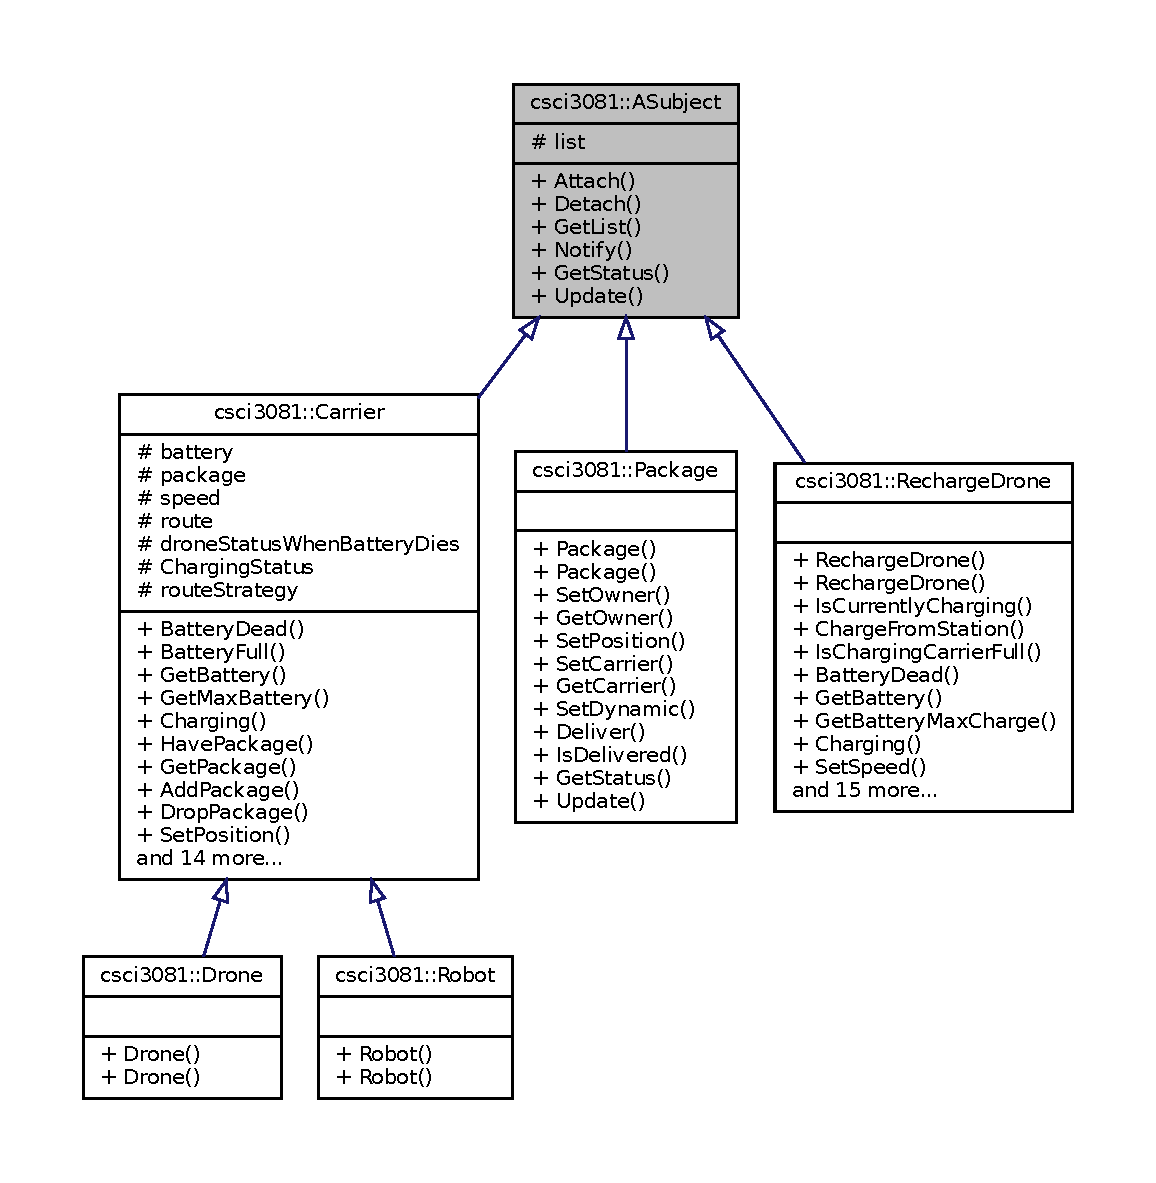
\includegraphics[width=350pt]{classcsci3081_1_1ASubject__inherit__graph}
\end{center}
\end{figure}
\subsection*{Public Member Functions}
\begin{DoxyCompactItemize}
\item 
void \hyperlink{classcsci3081_1_1ASubject_a8a04b98cb169de561a8a861baf82c8c3}{Attach} (\hyperlink{classentity__project_1_1IEntityObserver}{entity\+\_\+project\+::\+I\+Entity\+Observer} $\ast$observer)
\begin{DoxyCompactList}\small\item\em Adds an observer to the list of observers for this subject. \end{DoxyCompactList}\item 
void \hyperlink{classcsci3081_1_1ASubject_ae077b42d8551ecf10c587250a6c46cc2}{Detach} (\hyperlink{classentity__project_1_1IEntityObserver}{entity\+\_\+project\+::\+I\+Entity\+Observer} $\ast$observer)
\begin{DoxyCompactList}\small\item\em Deletes an observer from the list of observers for this subject. \end{DoxyCompactList}\item 
std\+::vector$<$ \hyperlink{classentity__project_1_1IEntityObserver}{entity\+\_\+project\+::\+I\+Entity\+Observer} $\ast$ $>$ \hyperlink{classcsci3081_1_1ASubject_aaa18e3aab659fe04b75dd6cba8efd4fa}{Get\+List} ()
\begin{DoxyCompactList}\small\item\em Getter function for the list of observers (mostly used in testing) \end{DoxyCompactList}\item 
void \hyperlink{classcsci3081_1_1ASubject_a2f219d68c9fc28373bb6f5e90170b4ae}{Notify} (picojson\+::value \&event, const \hyperlink{classentity__project_1_1IEntity}{entity\+\_\+project\+::\+I\+Entity} \&entity)
\begin{DoxyCompactList}\small\item\em Sends out Notification to the observer watching this subject. \end{DoxyCompactList}\item 
virtual void \hyperlink{classcsci3081_1_1ASubject_a206a9ddb559da279011e2f9ea29663dc}{Get\+Status} ()=0
\begin{DoxyCompactList}\small\item\em Pure virtual function Get\+Status that needs to implemented by derived class based on their types of notification. This function creates the arguments required by Notify function and makes call to Notify function. \end{DoxyCompactList}\item 
virtual void \hyperlink{classcsci3081_1_1ASubject_a04fdda736b2eb2784e5ef10d5f70dc7a}{Update} (float dt)=0
\begin{DoxyCompactList}\small\item\em Pure virtual function Update that needs to implemented by derived class based on their entity type. This function is used to advance time in the simulation. \end{DoxyCompactList}\end{DoxyCompactItemize}
\subsection*{Protected Attributes}
\begin{DoxyCompactItemize}
\item 
\mbox{\Hypertarget{classcsci3081_1_1ASubject_a3babfe8bff88a50ce4ce30973f2c5003}\label{classcsci3081_1_1ASubject_a3babfe8bff88a50ce4ce30973f2c5003}} 
std\+::vector$<$ \hyperlink{classentity__project_1_1IEntityObserver}{entity\+\_\+project\+::\+I\+Entity\+Observer} $\ast$ $>$ \hyperlink{classcsci3081_1_1ASubject_a3babfe8bff88a50ce4ce30973f2c5003}{list}
\begin{DoxyCompactList}\small\item\em List of pointers to the observers for this subject. \end{DoxyCompactList}\end{DoxyCompactItemize}


\subsection{Detailed Description}
This is the Abstract Subject class from which our subjects will inherit Implements the Observer/subject pattern. 

\subsection{Member Function Documentation}
\mbox{\Hypertarget{classcsci3081_1_1ASubject_a8a04b98cb169de561a8a861baf82c8c3}\label{classcsci3081_1_1ASubject_a8a04b98cb169de561a8a861baf82c8c3}} 
\index{csci3081\+::\+A\+Subject@{csci3081\+::\+A\+Subject}!Attach@{Attach}}
\index{Attach@{Attach}!csci3081\+::\+A\+Subject@{csci3081\+::\+A\+Subject}}
\subsubsection{\texorpdfstring{Attach()}{Attach()}}
{\footnotesize\ttfamily void csci3081\+::\+A\+Subject\+::\+Attach (\begin{DoxyParamCaption}\item[{\hyperlink{classentity__project_1_1IEntityObserver}{entity\+\_\+project\+::\+I\+Entity\+Observer} $\ast$}]{observer }\end{DoxyParamCaption})}



Adds an observer to the list of observers for this subject. 


\begin{DoxyParams}{Parameters}
{\em I\+Entity\+Observer$\ast$} & observer \\
\hline
\end{DoxyParams}
\mbox{\Hypertarget{classcsci3081_1_1ASubject_ae077b42d8551ecf10c587250a6c46cc2}\label{classcsci3081_1_1ASubject_ae077b42d8551ecf10c587250a6c46cc2}} 
\index{csci3081\+::\+A\+Subject@{csci3081\+::\+A\+Subject}!Detach@{Detach}}
\index{Detach@{Detach}!csci3081\+::\+A\+Subject@{csci3081\+::\+A\+Subject}}
\subsubsection{\texorpdfstring{Detach()}{Detach()}}
{\footnotesize\ttfamily void csci3081\+::\+A\+Subject\+::\+Detach (\begin{DoxyParamCaption}\item[{\hyperlink{classentity__project_1_1IEntityObserver}{entity\+\_\+project\+::\+I\+Entity\+Observer} $\ast$}]{observer }\end{DoxyParamCaption})}



Deletes an observer from the list of observers for this subject. 


\begin{DoxyParams}{Parameters}
{\em I\+Entity\+Observer$\ast$} & observer \\
\hline
\end{DoxyParams}
\mbox{\Hypertarget{classcsci3081_1_1ASubject_aaa18e3aab659fe04b75dd6cba8efd4fa}\label{classcsci3081_1_1ASubject_aaa18e3aab659fe04b75dd6cba8efd4fa}} 
\index{csci3081\+::\+A\+Subject@{csci3081\+::\+A\+Subject}!Get\+List@{Get\+List}}
\index{Get\+List@{Get\+List}!csci3081\+::\+A\+Subject@{csci3081\+::\+A\+Subject}}
\subsubsection{\texorpdfstring{Get\+List()}{GetList()}}
{\footnotesize\ttfamily std\+::vector$<$ \hyperlink{classentity__project_1_1IEntityObserver}{entity\+\_\+project\+::\+I\+Entity\+Observer} $\ast$ $>$ csci3081\+::\+A\+Subject\+::\+Get\+List (\begin{DoxyParamCaption}{ }\end{DoxyParamCaption})}



Getter function for the list of observers (mostly used in testing) 

\begin{DoxyReturn}{Returns}
std\+::vector $<$\hyperlink{classentity__project_1_1IEntityObserver}{entity\+\_\+project\+::\+I\+Entity\+Observer}$\ast$$>$ list 
\end{DoxyReturn}
\mbox{\Hypertarget{classcsci3081_1_1ASubject_a206a9ddb559da279011e2f9ea29663dc}\label{classcsci3081_1_1ASubject_a206a9ddb559da279011e2f9ea29663dc}} 
\index{csci3081\+::\+A\+Subject@{csci3081\+::\+A\+Subject}!Get\+Status@{Get\+Status}}
\index{Get\+Status@{Get\+Status}!csci3081\+::\+A\+Subject@{csci3081\+::\+A\+Subject}}
\subsubsection{\texorpdfstring{Get\+Status()}{GetStatus()}}
{\footnotesize\ttfamily virtual void csci3081\+::\+A\+Subject\+::\+Get\+Status (\begin{DoxyParamCaption}{ }\end{DoxyParamCaption})\hspace{0.3cm}{\ttfamily [pure virtual]}}



Pure virtual function Get\+Status that needs to implemented by derived class based on their types of notification. This function creates the arguments required by Notify function and makes call to Notify function. 


\begin{DoxyParams}{Parameters}
{\em picojson\+::value\&} & event \\
\hline
{\em const} & \hyperlink{classentity__project_1_1IEntity}{entity\+\_\+project\+::\+I\+Entity}\& entity \\
\hline
\end{DoxyParams}


Implemented in \hyperlink{classcsci3081_1_1RechargeDrone_aa245b79215b39c86c1f9fde874bdf264}{csci3081\+::\+Recharge\+Drone}, \hyperlink{classcsci3081_1_1Carrier_a2b96f30454fee0766a5ed3a26fbf092c}{csci3081\+::\+Carrier}, and \hyperlink{classcsci3081_1_1Package_aaf2a9604fc4d3dd108e4b4002751be05}{csci3081\+::\+Package}.

\mbox{\Hypertarget{classcsci3081_1_1ASubject_a2f219d68c9fc28373bb6f5e90170b4ae}\label{classcsci3081_1_1ASubject_a2f219d68c9fc28373bb6f5e90170b4ae}} 
\index{csci3081\+::\+A\+Subject@{csci3081\+::\+A\+Subject}!Notify@{Notify}}
\index{Notify@{Notify}!csci3081\+::\+A\+Subject@{csci3081\+::\+A\+Subject}}
\subsubsection{\texorpdfstring{Notify()}{Notify()}}
{\footnotesize\ttfamily void csci3081\+::\+A\+Subject\+::\+Notify (\begin{DoxyParamCaption}\item[{picojson\+::value \&}]{event,  }\item[{const \hyperlink{classentity__project_1_1IEntity}{entity\+\_\+project\+::\+I\+Entity} \&}]{entity }\end{DoxyParamCaption})}



Sends out Notification to the observer watching this subject. 


\begin{DoxyParams}{Parameters}
{\em picojson\+::value\&} & event \\
\hline
{\em const} & \hyperlink{classentity__project_1_1IEntity}{entity\+\_\+project\+::\+I\+Entity}\& entity \\
\hline
\end{DoxyParams}
\mbox{\Hypertarget{classcsci3081_1_1ASubject_a04fdda736b2eb2784e5ef10d5f70dc7a}\label{classcsci3081_1_1ASubject_a04fdda736b2eb2784e5ef10d5f70dc7a}} 
\index{csci3081\+::\+A\+Subject@{csci3081\+::\+A\+Subject}!Update@{Update}}
\index{Update@{Update}!csci3081\+::\+A\+Subject@{csci3081\+::\+A\+Subject}}
\subsubsection{\texorpdfstring{Update()}{Update()}}
{\footnotesize\ttfamily virtual void csci3081\+::\+A\+Subject\+::\+Update (\begin{DoxyParamCaption}\item[{float}]{dt }\end{DoxyParamCaption})\hspace{0.3cm}{\ttfamily [pure virtual]}}



Pure virtual function Update that needs to implemented by derived class based on their entity type. This function is used to advance time in the simulation. 


\begin{DoxyParams}{Parameters}
{\em float} & dt refers to the amount of time the update call should advance the simulation by. For instance if a drone moves 1 unit of distance per unit of time, and Update is called with dt=.05, then the drone should move 1 $\ast$ .05 = .05 units of distance.\\
\hline
\end{DoxyParams}
Some things that should happen in the Update function\+: move drones, check if packages have been delivered to customers, etc. 

Implemented in \hyperlink{classcsci3081_1_1Carrier_a5f202411aa049586514a48129b959ed7}{csci3081\+::\+Carrier}, \hyperlink{classcsci3081_1_1RechargeDrone_ac4b45136e2969ac25941d46a8ccdb83a}{csci3081\+::\+Recharge\+Drone}, and \hyperlink{classcsci3081_1_1Package_acd1f198a6e087c08e1cfeed0f44a90be}{csci3081\+::\+Package}.



The documentation for this class was generated from the following files\+:\begin{DoxyCompactItemize}
\item 
/home/user/repo/project/include/asubject.\+h\item 
/home/user/repo/project/src/asubject.\+cc\end{DoxyCompactItemize}

\hypertarget{classcsci3081_1_1Battery}{}\section{csci3081\+:\+:Battery Class Reference}
\label{classcsci3081_1_1Battery}\index{csci3081\+::\+Battery@{csci3081\+::\+Battery}}
\subsection*{Public Member Functions}
\begin{DoxyCompactItemize}
\item 
\mbox{\Hypertarget{classcsci3081_1_1Battery_a7ac32ee83e3d7b87b8ddc0cfd42d8088}\label{classcsci3081_1_1Battery_a7ac32ee83e3d7b87b8ddc0cfd42d8088}} 
\hyperlink{classcsci3081_1_1Battery_a7ac32ee83e3d7b87b8ddc0cfd42d8088}{Battery} ()
\begin{DoxyCompactList}\small\item\em Default Constructor. This sets up an instance of \hyperlink{classcsci3081_1_1Battery}{Battery} with empty remaining life. \end{DoxyCompactList}\item 
\hyperlink{classcsci3081_1_1Battery_a523da2c50bea66ea0d4aa49a7688a385}{Battery} (float remaining\+Lifein\+Sec\+\_\+, std\+::string battery\+Type=\char`\"{}carrier\char`\"{})
\begin{DoxyCompactList}\small\item\em Constructor to set up an instance of \hyperlink{classcsci3081_1_1Battery}{Battery} with passing remaining life. \end{DoxyCompactList}\item 
float \hyperlink{classcsci3081_1_1Battery_a6233a4d2c5c11d9db3db41db3c3c675c}{Get\+Remaining\+Life} ()
\item 
float \hyperlink{classcsci3081_1_1Battery_af9e2a6131a7a1a0db66b95a3610e7db2}{Get\+Max\+Charge} ()
\item 
int \hyperlink{classcsci3081_1_1Battery_a68eb2bc2fdd001fa025f44374d6edc69}{Get\+Display\+Bar} ()
\item 
int \hyperlink{classcsci3081_1_1Battery_a2ea2113b8dbea215849c5446eb96134e}{Get\+Id} ()
\item 
void \hyperlink{classcsci3081_1_1Battery_a5a31b2b3b97718db96a9aeaaca1a4cc6}{Depleting} (float sec)
\begin{DoxyCompactList}\small\item\em Depleting The \hyperlink{classcsci3081_1_1Battery}{Battery}. Should be used everytime the object using battery is in action. \end{DoxyCompactList}\item 
bool \hyperlink{classcsci3081_1_1Battery_add69602a44edb56918384d3c24888e20}{Charging} (float sec)
\begin{DoxyCompactList}\small\item\em Charging The \hyperlink{classcsci3081_1_1Battery}{Battery}. \end{DoxyCompactList}\item 
\mbox{\Hypertarget{classcsci3081_1_1Battery_a03b38835791a378ac3374efbb3993eb4}\label{classcsci3081_1_1Battery_a03b38835791a378ac3374efbb3993eb4}} 
float \hyperlink{classcsci3081_1_1Battery_a03b38835791a378ac3374efbb3993eb4}{Time\+To\+Full} ()
\begin{DoxyCompactList}\small\item\em This function returns the time battery needed charged to be full. \end{DoxyCompactList}\item 
\mbox{\Hypertarget{classcsci3081_1_1Battery_a76a8b9485a8b901eed3e45cb738380cc}\label{classcsci3081_1_1Battery_a76a8b9485a8b901eed3e45cb738380cc}} 
bool \hyperlink{classcsci3081_1_1Battery_a76a8b9485a8b901eed3e45cb738380cc}{Is\+Dead} ()
\begin{DoxyCompactList}\small\item\em This returns a boolean value for the battery\textquotesingle{}s life False if battery is dead (below 20\%) True otherwise. \end{DoxyCompactList}\item 
\mbox{\Hypertarget{classcsci3081_1_1Battery_a04760ee4be9a947c7478e7da48e2f75e}\label{classcsci3081_1_1Battery_a04760ee4be9a947c7478e7da48e2f75e}} 
bool \hyperlink{classcsci3081_1_1Battery_a04760ee4be9a947c7478e7da48e2f75e}{Is\+Full} ()
\begin{DoxyCompactList}\small\item\em This returns a boolean value if the battery is full. True if the battery is full. False otherwise. \end{DoxyCompactList}\end{DoxyCompactItemize}


\subsection{Constructor \& Destructor Documentation}
\mbox{\Hypertarget{classcsci3081_1_1Battery_a523da2c50bea66ea0d4aa49a7688a385}\label{classcsci3081_1_1Battery_a523da2c50bea66ea0d4aa49a7688a385}} 
\index{csci3081\+::\+Battery@{csci3081\+::\+Battery}!Battery@{Battery}}
\index{Battery@{Battery}!csci3081\+::\+Battery@{csci3081\+::\+Battery}}
\subsubsection{\texorpdfstring{Battery()}{Battery()}}
{\footnotesize\ttfamily csci3081\+::\+Battery\+::\+Battery (\begin{DoxyParamCaption}\item[{float}]{remaining\+Lifein\+Sec\+\_\+,  }\item[{std\+::string}]{battery\+Type = {\ttfamily \char`\"{}carrier\char`\"{}} }\end{DoxyParamCaption})}



Constructor to set up an instance of \hyperlink{classcsci3081_1_1Battery}{Battery} with passing remaining life. 


\begin{DoxyParams}[1]{Parameters}
\mbox{\tt in}  & {\em remaining\+Lifein\+Sec\+\_\+} & current remaining life in the battery \\
\hline
\mbox{\tt in}  & {\em battery\+Type} & optional; there are 2 types of batteries\+: carrier and recharging\+\_\+drone. Recharging drone has higher max\+Charge than carrier. Default of batter\+Type is carrier. \\
\hline
\end{DoxyParams}


\subsection{Member Function Documentation}
\mbox{\Hypertarget{classcsci3081_1_1Battery_add69602a44edb56918384d3c24888e20}\label{classcsci3081_1_1Battery_add69602a44edb56918384d3c24888e20}} 
\index{csci3081\+::\+Battery@{csci3081\+::\+Battery}!Charging@{Charging}}
\index{Charging@{Charging}!csci3081\+::\+Battery@{csci3081\+::\+Battery}}
\subsubsection{\texorpdfstring{Charging()}{Charging()}}
{\footnotesize\ttfamily bool csci3081\+::\+Battery\+::\+Charging (\begin{DoxyParamCaption}\item[{float}]{sec }\end{DoxyParamCaption})}



Charging The \hyperlink{classcsci3081_1_1Battery}{Battery}. 


\begin{DoxyParams}[1]{Parameters}
\mbox{\tt in}  & {\em sec} & seconds battery is charged \\
\hline
\mbox{\tt out}  & {\em True} & if the battery is charged, False otherwise \\
\hline
\end{DoxyParams}
\mbox{\Hypertarget{classcsci3081_1_1Battery_a5a31b2b3b97718db96a9aeaaca1a4cc6}\label{classcsci3081_1_1Battery_a5a31b2b3b97718db96a9aeaaca1a4cc6}} 
\index{csci3081\+::\+Battery@{csci3081\+::\+Battery}!Depleting@{Depleting}}
\index{Depleting@{Depleting}!csci3081\+::\+Battery@{csci3081\+::\+Battery}}
\subsubsection{\texorpdfstring{Depleting()}{Depleting()}}
{\footnotesize\ttfamily void csci3081\+::\+Battery\+::\+Depleting (\begin{DoxyParamCaption}\item[{float}]{sec }\end{DoxyParamCaption})}



Depleting The \hyperlink{classcsci3081_1_1Battery}{Battery}. Should be used everytime the object using battery is in action. 


\begin{DoxyParams}[1]{Parameters}
\mbox{\tt in}  & {\em sec} & seconds battery is used \\
\hline
\end{DoxyParams}
\mbox{\Hypertarget{classcsci3081_1_1Battery_a68eb2bc2fdd001fa025f44374d6edc69}\label{classcsci3081_1_1Battery_a68eb2bc2fdd001fa025f44374d6edc69}} 
\index{csci3081\+::\+Battery@{csci3081\+::\+Battery}!Get\+Display\+Bar@{Get\+Display\+Bar}}
\index{Get\+Display\+Bar@{Get\+Display\+Bar}!csci3081\+::\+Battery@{csci3081\+::\+Battery}}
\subsubsection{\texorpdfstring{Get\+Display\+Bar()}{GetDisplayBar()}}
{\footnotesize\ttfamily int csci3081\+::\+Battery\+::\+Get\+Display\+Bar (\begin{DoxyParamCaption}{ }\end{DoxyParamCaption})}

This functions return the current display\+Bar of the \hyperlink{classcsci3081_1_1Battery}{Battery} \mbox{\Hypertarget{classcsci3081_1_1Battery_a2ea2113b8dbea215849c5446eb96134e}\label{classcsci3081_1_1Battery_a2ea2113b8dbea215849c5446eb96134e}} 
\index{csci3081\+::\+Battery@{csci3081\+::\+Battery}!Get\+Id@{Get\+Id}}
\index{Get\+Id@{Get\+Id}!csci3081\+::\+Battery@{csci3081\+::\+Battery}}
\subsubsection{\texorpdfstring{Get\+Id()}{GetId()}}
{\footnotesize\ttfamily int csci3081\+::\+Battery\+::\+Get\+Id (\begin{DoxyParamCaption}{ }\end{DoxyParamCaption})}

This functions return the ID of the battery \mbox{\Hypertarget{classcsci3081_1_1Battery_af9e2a6131a7a1a0db66b95a3610e7db2}\label{classcsci3081_1_1Battery_af9e2a6131a7a1a0db66b95a3610e7db2}} 
\index{csci3081\+::\+Battery@{csci3081\+::\+Battery}!Get\+Max\+Charge@{Get\+Max\+Charge}}
\index{Get\+Max\+Charge@{Get\+Max\+Charge}!csci3081\+::\+Battery@{csci3081\+::\+Battery}}
\subsubsection{\texorpdfstring{Get\+Max\+Charge()}{GetMaxCharge()}}
{\footnotesize\ttfamily float csci3081\+::\+Battery\+::\+Get\+Max\+Charge (\begin{DoxyParamCaption}{ }\end{DoxyParamCaption})}

This function returns the max charge of the battery. \mbox{\Hypertarget{classcsci3081_1_1Battery_a6233a4d2c5c11d9db3db41db3c3c675c}\label{classcsci3081_1_1Battery_a6233a4d2c5c11d9db3db41db3c3c675c}} 
\index{csci3081\+::\+Battery@{csci3081\+::\+Battery}!Get\+Remaining\+Life@{Get\+Remaining\+Life}}
\index{Get\+Remaining\+Life@{Get\+Remaining\+Life}!csci3081\+::\+Battery@{csci3081\+::\+Battery}}
\subsubsection{\texorpdfstring{Get\+Remaining\+Life()}{GetRemainingLife()}}
{\footnotesize\ttfamily float csci3081\+::\+Battery\+::\+Get\+Remaining\+Life (\begin{DoxyParamCaption}{ }\end{DoxyParamCaption})}

This functions return the remaining life of the battery 

The documentation for this class was generated from the following files\+:\begin{DoxyCompactItemize}
\item 
/home/user/repo/project/include/battery.\+h\item 
/home/user/repo/project/src/battery.\+cc\end{DoxyCompactItemize}

\hypertarget{classcsci3081_1_1BeelineRoute}{}\section{csci3081\+:\+:Beeline\+Route Class Reference}
\label{classcsci3081_1_1BeelineRoute}\index{csci3081\+::\+Beeline\+Route@{csci3081\+::\+Beeline\+Route}}


This is the Beeline Route class where we can use the strategy pattern to implement a Beeline route for carriers.  




{\ttfamily \#include $<$beeline\+\_\+route.\+h$>$}



Inheritance diagram for csci3081\+:\+:Beeline\+Route\+:
\nopagebreak
\begin{figure}[H]
\begin{center}
\leavevmode
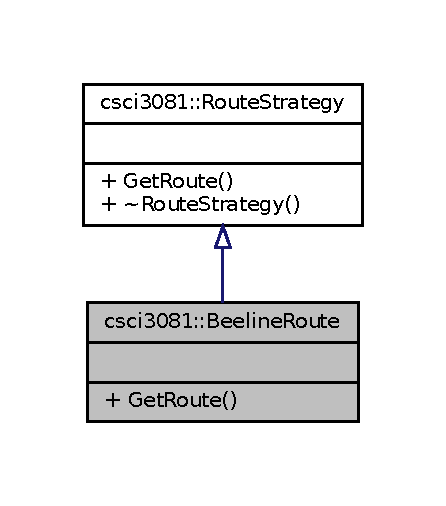
\includegraphics[width=214pt]{classcsci3081_1_1BeelineRoute__inherit__graph}
\end{center}
\end{figure}
\subsection*{Public Member Functions}
\begin{DoxyCompactItemize}
\item 
std\+::vector$<$ std\+::vector$<$ float $>$ $>$ \hyperlink{classcsci3081_1_1BeelineRoute_a38aacbeafb14145e807c60990199785c}{Get\+Route} (const \hyperlink{classentity__project_1_1IGraph}{I\+Graph} $\ast$graph, std\+::vector$<$ float $>$ location, std\+::vector$<$ float $>$ dest)
\begin{DoxyCompactList}\small\item\em This function allows the moving item to get the desired route. In this class, the function will return a route that follows the Beeline path. \end{DoxyCompactList}\end{DoxyCompactItemize}


\subsection{Detailed Description}
This is the Beeline Route class where we can use the strategy pattern to implement a Beeline route for carriers. 

\subsection{Member Function Documentation}
\mbox{\Hypertarget{classcsci3081_1_1BeelineRoute_a38aacbeafb14145e807c60990199785c}\label{classcsci3081_1_1BeelineRoute_a38aacbeafb14145e807c60990199785c}} 
\index{csci3081\+::\+Beeline\+Route@{csci3081\+::\+Beeline\+Route}!Get\+Route@{Get\+Route}}
\index{Get\+Route@{Get\+Route}!csci3081\+::\+Beeline\+Route@{csci3081\+::\+Beeline\+Route}}
\subsubsection{\texorpdfstring{Get\+Route()}{GetRoute()}}
{\footnotesize\ttfamily std\+::vector$<$ std\+::vector$<$ float $>$ $>$ csci3081\+::\+Beeline\+Route\+::\+Get\+Route (\begin{DoxyParamCaption}\item[{const \hyperlink{classentity__project_1_1IGraph}{I\+Graph} $\ast$}]{graph,  }\item[{std\+::vector$<$ float $>$}]{location,  }\item[{std\+::vector$<$ float $>$}]{dest }\end{DoxyParamCaption})\hspace{0.3cm}{\ttfamily [virtual]}}



This function allows the moving item to get the desired route. In this class, the function will return a route that follows the Beeline path. 

The route includes a point where the drone needs to go up to by a certain height from where it is at, then another point to the destination location with the same certain height, then another point to the final destination location.


\begin{DoxyParams}{Parameters}
{\em const} & I\+Graph$\ast$ graph; we don\textquotesingle{}t need to use this parameter \\
\hline
{\em std\+::vector$<$float$>$} & location Current drone location \\
\hline
{\em std\+::vector$<$float$>$} & dest Final location where the drone needs to be \\
\hline
\end{DoxyParams}
\begin{DoxyReturn}{Returns}
std\+::vector $<$std\+::vector$<$float$>$$>$ The path of the beeline 
\end{DoxyReturn}


Implements \hyperlink{classcsci3081_1_1RouteStrategy_a4bf67b185a4446324ebc13c1cda40cfe}{csci3081\+::\+Route\+Strategy}.



The documentation for this class was generated from the following files\+:\begin{DoxyCompactItemize}
\item 
/home/user/repo/project/include/beeline\+\_\+route.\+h\item 
/home/user/repo/project/src/beeline\+\_\+route.\+cc\end{DoxyCompactItemize}

\hypertarget{classcsci3081_1_1Carrier}{}\section{csci3081\+:\+:Carrier Class Reference}
\label{classcsci3081_1_1Carrier}\index{csci3081\+::\+Carrier@{csci3081\+::\+Carrier}}


A representation of a carrier An abstract base class for delivery transportation clases like \hyperlink{classcsci3081_1_1Drone}{Drone} or \hyperlink{classcsci3081_1_1Robot}{Robot}. \hyperlink{classcsci3081_1_1Robot}{Robot} and \hyperlink{classcsci3081_1_1Drone}{Drone} inherited from \hyperlink{classcsci3081_1_1Carrier}{Carrier}.  




{\ttfamily \#include $<$carrier.\+h$>$}



Inheritance diagram for csci3081\+:\+:Carrier\+:
\nopagebreak
\begin{figure}[H]
\begin{center}
\leavevmode
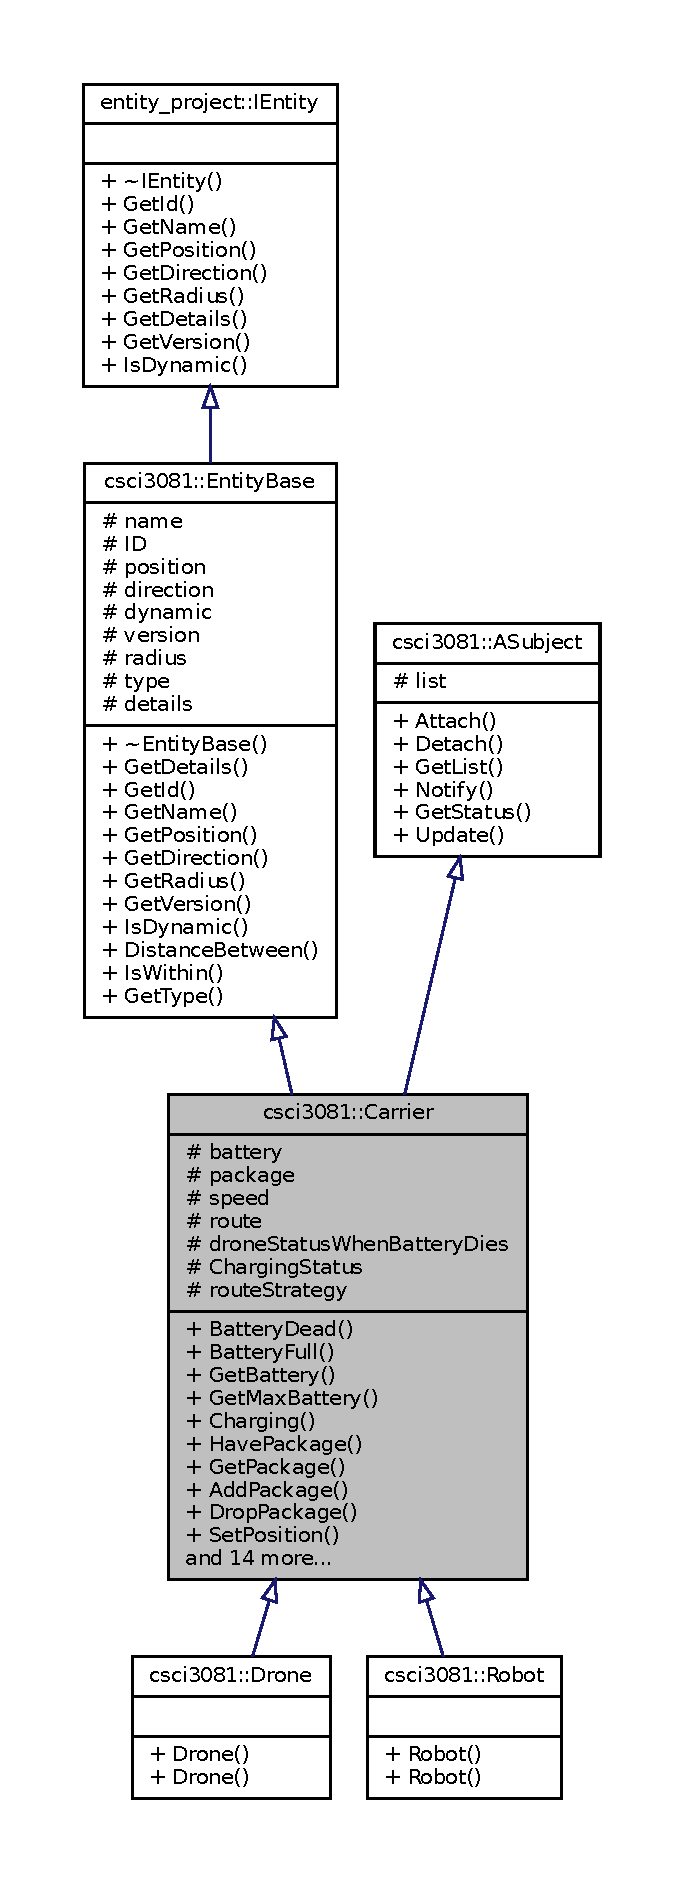
\includegraphics[height=550pt]{classcsci3081_1_1Carrier__inherit__graph}
\end{center}
\end{figure}
\subsection*{Public Member Functions}
\begin{DoxyCompactItemize}
\item 
bool \hyperlink{classcsci3081_1_1Carrier_abbf8f72d3b13da90793555e25053d793}{Battery\+Dead} ()
\begin{DoxyCompactList}\small\item\em This checks if the carrier is out of battery. \end{DoxyCompactList}\item 
bool \hyperlink{classcsci3081_1_1Carrier_aaeb0a45df6b9fa522e04681da272cb6f}{Battery\+Full} ()
\begin{DoxyCompactList}\small\item\em This function checks if the battery is full. \end{DoxyCompactList}\item 
\mbox{\Hypertarget{classcsci3081_1_1Carrier_ad8e833d85c22f1f516646360aa852338}\label{classcsci3081_1_1Carrier_ad8e833d85c22f1f516646360aa852338}} 
float \hyperlink{classcsci3081_1_1Carrier_ad8e833d85c22f1f516646360aa852338}{Get\+Battery} ()
\begin{DoxyCompactList}\small\item\em This returns the time in secs left in the carrier\textquotesingle{}s battery. \end{DoxyCompactList}\item 
\mbox{\Hypertarget{classcsci3081_1_1Carrier_a5935ddc44bb01290fe65168332d5a811}\label{classcsci3081_1_1Carrier_a5935ddc44bb01290fe65168332d5a811}} 
float \hyperlink{classcsci3081_1_1Carrier_a5935ddc44bb01290fe65168332d5a811}{Get\+Max\+Battery} ()
\begin{DoxyCompactList}\small\item\em This returns the battery maximum capacity. \end{DoxyCompactList}\item 
bool \hyperlink{classcsci3081_1_1Carrier_aa004703e60b8ffed9661ee204f619983}{Charging} (float)
\begin{DoxyCompactList}\small\item\em This function is used to charge the battery of the carrier for a certain amount of time in seconds. \end{DoxyCompactList}\item 
bool \hyperlink{classcsci3081_1_1Carrier_a5f20ff445085ba10866ff83dc3d2ea93}{Have\+Package} ()
\begin{DoxyCompactList}\small\item\em This checks if the carrier is already linked to a package. \end{DoxyCompactList}\item 
\mbox{\Hypertarget{classcsci3081_1_1Carrier_a8938441bb8d2984178eb75b4ce45e6b9}\label{classcsci3081_1_1Carrier_a8938441bb8d2984178eb75b4ce45e6b9}} 
\hyperlink{classcsci3081_1_1Package}{Package} $\ast$ \hyperlink{classcsci3081_1_1Carrier_a8938441bb8d2984178eb75b4ce45e6b9}{Get\+Package} ()
\begin{DoxyCompactList}\small\item\em This returns a \hyperlink{classcsci3081_1_1Package}{Package} pointer to the package that the carrier is linking to, and returns N\+U\+LL if the carrier is not linking to any package. \end{DoxyCompactList}\item 
bool \hyperlink{classcsci3081_1_1Carrier_a8b1996acbdeb796bcbc68f8d092e09c0}{Add\+Package} (\hyperlink{classcsci3081_1_1Package}{Package} $\ast$arg)
\begin{DoxyCompactList}\small\item\em This links a package object to the carrier if the carrier is not already linking to another package (carrier can only carry one package at a time) \end{DoxyCompactList}\item 
\hyperlink{classcsci3081_1_1Package}{Package} $\ast$ \hyperlink{classcsci3081_1_1Carrier_a6fa3861b1b7acb89827e768308196cc1}{Drop\+Package} ()
\begin{DoxyCompactList}\small\item\em This releases the link of the package from the carrier, making the package pointer of the carrier N\+U\+LL, and return a pointer to the just dropped/delivered package. \end{DoxyCompactList}\item 
void \hyperlink{classcsci3081_1_1Carrier_aede9d79fffb164f90fe30b19f2e2c854}{Set\+Position} (std\+::vector$<$ float $>$ v)
\begin{DoxyCompactList}\small\item\em This function uses to set the new position of the carrier. However, carrier only moves in simulation if its dynamic attribute is set to true. \end{DoxyCompactList}\item 
void \hyperlink{classcsci3081_1_1Carrier_a1f74a376887685a69b3d0512eb97188e}{Set\+Speed} (float)
\begin{DoxyCompactList}\small\item\em This sets the speed of the carrier. Change the speed of the carrier if the argument is a non-\/negative float number. \end{DoxyCompactList}\item 
\mbox{\Hypertarget{classcsci3081_1_1Carrier_ab290cc18c82e6104dc1d3e3fa94ec3ff}\label{classcsci3081_1_1Carrier_ab290cc18c82e6104dc1d3e3fa94ec3ff}} 
float \hyperlink{classcsci3081_1_1Carrier_ab290cc18c82e6104dc1d3e3fa94ec3ff}{Get\+Speed} ()
\begin{DoxyCompactList}\small\item\em return the current speed of the carrier \end{DoxyCompactList}\item 
void \hyperlink{classcsci3081_1_1Carrier_a0b8c743cb8ab7843a4cece11225634f4}{Set\+Route} (std\+::vector$<$ vector$<$ float $>$$>$)
\begin{DoxyCompactList}\small\item\em This function adds a full route to route attribute of the carrier This is useful when use for the Get\+Path() function from I\+Graph class. \end{DoxyCompactList}\item 
\mbox{\Hypertarget{classcsci3081_1_1Carrier_a41a796fd2ee1261ad61dd87e1d4ed54f}\label{classcsci3081_1_1Carrier_a41a796fd2ee1261ad61dd87e1d4ed54f}} 
std\+::vector$<$ float $>$ \hyperlink{classcsci3081_1_1Carrier_a41a796fd2ee1261ad61dd87e1d4ed54f}{Next\+Position} ()
\begin{DoxyCompactList}\small\item\em This function returns the next position in std\+::vector$<$float$>$ in the queue that the carrier needs to move to. \end{DoxyCompactList}\item 
\mbox{\Hypertarget{classcsci3081_1_1Carrier_aa181fd3d4bf00e9800c9ddea28930523}\label{classcsci3081_1_1Carrier_aa181fd3d4bf00e9800c9ddea28930523}} 
void \hyperlink{classcsci3081_1_1Carrier_aa181fd3d4bf00e9800c9ddea28930523}{Pop\+Position} ()
\begin{DoxyCompactList}\small\item\em This function pops the first element/position in the position queue of the carrier. \end{DoxyCompactList}\item 
void \hyperlink{classcsci3081_1_1Carrier_a2b96f30454fee0766a5ed3a26fbf092c}{Get\+Status} ()
\begin{DoxyCompactList}\small\item\em Overwritten Get\+Status from \hyperlink{classcsci3081_1_1ASubject}{A\+Subject}. This function creates the arguments required by Notify function and makes call to Notify function. This function should be called when path is added to the carrier and when the carrier becomes idle. \end{DoxyCompactList}\item 
\mbox{\Hypertarget{classcsci3081_1_1Carrier_a871790b7d86cc3fc47c659131d752bfe}\label{classcsci3081_1_1Carrier_a871790b7d86cc3fc47c659131d752bfe}} 
\hyperlink{classcsci3081_1_1RouteStrategy}{Route\+Strategy} $\ast$ \hyperlink{classcsci3081_1_1Carrier_a871790b7d86cc3fc47c659131d752bfe}{Get\+Route\+Strategy} ()
\begin{DoxyCompactList}\small\item\em return the Route Strategy that the carrier uses, such as Smart Route, Beeline, or Parabolic Route \end{DoxyCompactList}\item 
bool \hyperlink{classcsci3081_1_1Carrier_ac126252e1b6bf129d4369b299851211d}{Is\+Currently\+Charging} ()
\begin{DoxyCompactList}\small\item\em This function checks if the carrier battery is currently charging. \end{DoxyCompactList}\item 
\hyperlink{classcsci3081_1_1Battery}{Battery} $\ast$ \hyperlink{classcsci3081_1_1Carrier_a0d871b65140eefec69158b14703d92bc}{Get\+Battery\+Obj} ()
\begin{DoxyCompactList}\small\item\em This function will return the \hyperlink{classcsci3081_1_1Battery}{Battery} object. \end{DoxyCompactList}\item 
void \hyperlink{classcsci3081_1_1Carrier_a10382f16402af20f4bc03eaad5eb9e30}{Set\+Charging\+Status} (bool b)
\begin{DoxyCompactList}\small\item\em This function sets the carrier battery status. \end{DoxyCompactList}\item 
void \hyperlink{classcsci3081_1_1Carrier_a039d932119b4b3b7e076ff9e6ffada80}{Set\+Drone\+Status\+When\+Battery\+Dies} (std\+::string status)
\begin{DoxyCompactList}\small\item\em This function sets the battery status when the battery dies (alive, dead on ground, or dead in the air) \end{DoxyCompactList}\item 
std\+::string \hyperlink{classcsci3081_1_1Carrier_a25d1396e9c91e9574ab752eaf0b24048}{Get\+Drone\+Status\+When\+Battery\+Dies} ()
\begin{DoxyCompactList}\small\item\em This function gets the battery status (alive, dead on ground, or dead in the air) \end{DoxyCompactList}\item 
\mbox{\Hypertarget{classcsci3081_1_1Carrier_ab09ba1ba2a316e0ef29458cc9c303afd}\label{classcsci3081_1_1Carrier_ab09ba1ba2a316e0ef29458cc9c303afd}} 
void \hyperlink{classcsci3081_1_1Carrier_ab09ba1ba2a316e0ef29458cc9c303afd}{Go\+Down\+To\+Ground} ()
\begin{DoxyCompactList}\small\item\em This function sends the carrier down (if on the air) to the ground when the battery is dead. If the carrier is currently delivering a package, it will drop its package for other available carriers to come and pick it up. \end{DoxyCompactList}\item 
\mbox{\Hypertarget{classcsci3081_1_1Carrier_a5f202411aa049586514a48129b959ed7}\label{classcsci3081_1_1Carrier_a5f202411aa049586514a48129b959ed7}} 
void \hyperlink{classcsci3081_1_1Carrier_a5f202411aa049586514a48129b959ed7}{Update} (float dt)
\begin{DoxyCompactList}\small\item\em This is an inherited method from \hyperlink{classcsci3081_1_1EntityBase}{Entity\+Base} to use for \hyperlink{classcsci3081_1_1DeliverySimulation}{Delivery\+Simulation}. This updates the position of the carrier on the simulation if the position changes and its dynamic is set to true. In addition, this function also checks if the carrier is in within distance with the package to pick it up, or within distance with the customer to drop off the package. \end{DoxyCompactList}\end{DoxyCompactItemize}
\subsection*{Protected Attributes}
\begin{DoxyCompactItemize}
\item 
\mbox{\Hypertarget{classcsci3081_1_1Carrier_a6d5a40dc3672b6b8667bac84a967dfc7}\label{classcsci3081_1_1Carrier_a6d5a40dc3672b6b8667bac84a967dfc7}} 
\hyperlink{classcsci3081_1_1Battery}{Battery} {\bfseries battery}
\item 
\mbox{\Hypertarget{classcsci3081_1_1Carrier_abe593b696584b20307c5eb7fb9184aff}\label{classcsci3081_1_1Carrier_abe593b696584b20307c5eb7fb9184aff}} 
\hyperlink{classcsci3081_1_1Package}{Package} $\ast$ {\bfseries package}
\item 
\mbox{\Hypertarget{classcsci3081_1_1Carrier_abe394952b911bb17b1acfd88163c9c05}\label{classcsci3081_1_1Carrier_abe394952b911bb17b1acfd88163c9c05}} 
float {\bfseries speed}
\item 
\mbox{\Hypertarget{classcsci3081_1_1Carrier_ac2d6218c5d9856936c75b270e4e32be6}\label{classcsci3081_1_1Carrier_ac2d6218c5d9856936c75b270e4e32be6}} 
std\+::vector$<$ std\+::vector$<$ float $>$ $>$ {\bfseries route}
\item 
\mbox{\Hypertarget{classcsci3081_1_1Carrier_aa8d4466ebdba226c137122012a193633}\label{classcsci3081_1_1Carrier_aa8d4466ebdba226c137122012a193633}} 
std\+::string {\bfseries drone\+Status\+When\+Battery\+Dies} = \char`\"{}not dead yet\char`\"{}
\item 
\mbox{\Hypertarget{classcsci3081_1_1Carrier_aa689bdcb7d895a92ff802b39ab649b21}\label{classcsci3081_1_1Carrier_aa689bdcb7d895a92ff802b39ab649b21}} 
bool {\bfseries Charging\+Status} = false
\item 
\mbox{\Hypertarget{classcsci3081_1_1Carrier_a2fc7570deeaf96260542f0cb218225f2}\label{classcsci3081_1_1Carrier_a2fc7570deeaf96260542f0cb218225f2}} 
\hyperlink{classcsci3081_1_1RouteStrategy}{Route\+Strategy} $\ast$ {\bfseries route\+Strategy} = N\+U\+LL
\end{DoxyCompactItemize}


\subsection{Detailed Description}
A representation of a carrier An abstract base class for delivery transportation clases like \hyperlink{classcsci3081_1_1Drone}{Drone} or \hyperlink{classcsci3081_1_1Robot}{Robot}. \hyperlink{classcsci3081_1_1Robot}{Robot} and \hyperlink{classcsci3081_1_1Drone}{Drone} inherited from \hyperlink{classcsci3081_1_1Carrier}{Carrier}. 

\subsection{Member Function Documentation}
\mbox{\Hypertarget{classcsci3081_1_1Carrier_a8b1996acbdeb796bcbc68f8d092e09c0}\label{classcsci3081_1_1Carrier_a8b1996acbdeb796bcbc68f8d092e09c0}} 
\index{csci3081\+::\+Carrier@{csci3081\+::\+Carrier}!Add\+Package@{Add\+Package}}
\index{Add\+Package@{Add\+Package}!csci3081\+::\+Carrier@{csci3081\+::\+Carrier}}
\subsubsection{\texorpdfstring{Add\+Package()}{AddPackage()}}
{\footnotesize\ttfamily bool csci3081\+::\+Carrier\+::\+Add\+Package (\begin{DoxyParamCaption}\item[{\hyperlink{classcsci3081_1_1Package}{Package} $\ast$}]{arg }\end{DoxyParamCaption})}



This links a package object to the carrier if the carrier is not already linking to another package (carrier can only carry one package at a time) 


\begin{DoxyParams}[1]{Parameters}
\mbox{\tt in}  & {\em arg} & a \hyperlink{classcsci3081_1_1Package}{Package} pointer \\
\hline
\end{DoxyParams}
\begin{DoxyReturn}{Returns}
True upon succeeding linking the package to the carrier False otherwise (e.\+g. carrier is already linked to another package) 
\end{DoxyReturn}
\mbox{\Hypertarget{classcsci3081_1_1Carrier_abbf8f72d3b13da90793555e25053d793}\label{classcsci3081_1_1Carrier_abbf8f72d3b13da90793555e25053d793}} 
\index{csci3081\+::\+Carrier@{csci3081\+::\+Carrier}!Battery\+Dead@{Battery\+Dead}}
\index{Battery\+Dead@{Battery\+Dead}!csci3081\+::\+Carrier@{csci3081\+::\+Carrier}}
\subsubsection{\texorpdfstring{Battery\+Dead()}{BatteryDead()}}
{\footnotesize\ttfamily bool csci3081\+::\+Carrier\+::\+Battery\+Dead (\begin{DoxyParamCaption}{ }\end{DoxyParamCaption})}



This checks if the carrier is out of battery. 

\begin{DoxyReturn}{Returns}
T\+R\+UE if the battery of the carrier is out F\+A\+L\+SE otherwise 
\end{DoxyReturn}
\mbox{\Hypertarget{classcsci3081_1_1Carrier_aaeb0a45df6b9fa522e04681da272cb6f}\label{classcsci3081_1_1Carrier_aaeb0a45df6b9fa522e04681da272cb6f}} 
\index{csci3081\+::\+Carrier@{csci3081\+::\+Carrier}!Battery\+Full@{Battery\+Full}}
\index{Battery\+Full@{Battery\+Full}!csci3081\+::\+Carrier@{csci3081\+::\+Carrier}}
\subsubsection{\texorpdfstring{Battery\+Full()}{BatteryFull()}}
{\footnotesize\ttfamily bool csci3081\+::\+Carrier\+::\+Battery\+Full (\begin{DoxyParamCaption}{ }\end{DoxyParamCaption})}



This function checks if the battery is full. 

\begin{DoxyReturn}{Returns}
bool True if battery is full. False otherwise. 
\end{DoxyReturn}
\mbox{\Hypertarget{classcsci3081_1_1Carrier_aa004703e60b8ffed9661ee204f619983}\label{classcsci3081_1_1Carrier_aa004703e60b8ffed9661ee204f619983}} 
\index{csci3081\+::\+Carrier@{csci3081\+::\+Carrier}!Charging@{Charging}}
\index{Charging@{Charging}!csci3081\+::\+Carrier@{csci3081\+::\+Carrier}}
\subsubsection{\texorpdfstring{Charging()}{Charging()}}
{\footnotesize\ttfamily bool csci3081\+::\+Carrier\+::\+Charging (\begin{DoxyParamCaption}\item[{float}]{sec }\end{DoxyParamCaption})}



This function is used to charge the battery of the carrier for a certain amount of time in seconds. 


\begin{DoxyParams}[1]{Parameters}
\mbox{\tt in}  & {\em sec} & amount of time in secs to charge the battery \\
\hline
\end{DoxyParams}
\begin{DoxyReturn}{Returns}
T\+R\+UE if the battery can be charged F\+A\+L\+SE otherwise 
\end{DoxyReturn}
\mbox{\Hypertarget{classcsci3081_1_1Carrier_a6fa3861b1b7acb89827e768308196cc1}\label{classcsci3081_1_1Carrier_a6fa3861b1b7acb89827e768308196cc1}} 
\index{csci3081\+::\+Carrier@{csci3081\+::\+Carrier}!Drop\+Package@{Drop\+Package}}
\index{Drop\+Package@{Drop\+Package}!csci3081\+::\+Carrier@{csci3081\+::\+Carrier}}
\subsubsection{\texorpdfstring{Drop\+Package()}{DropPackage()}}
{\footnotesize\ttfamily \hyperlink{classcsci3081_1_1Package}{Package} $\ast$ csci3081\+::\+Carrier\+::\+Drop\+Package (\begin{DoxyParamCaption}{ }\end{DoxyParamCaption})}



This releases the link of the package from the carrier, making the package pointer of the carrier N\+U\+LL, and return a pointer to the just dropped/delivered package. 

\begin{DoxyReturn}{Returns}
a \hyperlink{classcsci3081_1_1Package}{Package} pointer to the just dropped/delivered package 
\end{DoxyReturn}
\mbox{\Hypertarget{classcsci3081_1_1Carrier_a0d871b65140eefec69158b14703d92bc}\label{classcsci3081_1_1Carrier_a0d871b65140eefec69158b14703d92bc}} 
\index{csci3081\+::\+Carrier@{csci3081\+::\+Carrier}!Get\+Battery\+Obj@{Get\+Battery\+Obj}}
\index{Get\+Battery\+Obj@{Get\+Battery\+Obj}!csci3081\+::\+Carrier@{csci3081\+::\+Carrier}}
\subsubsection{\texorpdfstring{Get\+Battery\+Obj()}{GetBatteryObj()}}
{\footnotesize\ttfamily \hyperlink{classcsci3081_1_1Battery}{Battery} $\ast$ csci3081\+::\+Carrier\+::\+Get\+Battery\+Obj (\begin{DoxyParamCaption}{ }\end{DoxyParamCaption})}



This function will return the \hyperlink{classcsci3081_1_1Battery}{Battery} object. 

\begin{DoxyReturn}{Returns}
\hyperlink{classcsci3081_1_1Battery}{Battery} \hyperlink{classcsci3081_1_1Battery}{Battery} in the drone 
\end{DoxyReturn}
\mbox{\Hypertarget{classcsci3081_1_1Carrier_a25d1396e9c91e9574ab752eaf0b24048}\label{classcsci3081_1_1Carrier_a25d1396e9c91e9574ab752eaf0b24048}} 
\index{csci3081\+::\+Carrier@{csci3081\+::\+Carrier}!Get\+Drone\+Status\+When\+Battery\+Dies@{Get\+Drone\+Status\+When\+Battery\+Dies}}
\index{Get\+Drone\+Status\+When\+Battery\+Dies@{Get\+Drone\+Status\+When\+Battery\+Dies}!csci3081\+::\+Carrier@{csci3081\+::\+Carrier}}
\subsubsection{\texorpdfstring{Get\+Drone\+Status\+When\+Battery\+Dies()}{GetDroneStatusWhenBatteryDies()}}
{\footnotesize\ttfamily std\+::string csci3081\+::\+Carrier\+::\+Get\+Drone\+Status\+When\+Battery\+Dies (\begin{DoxyParamCaption}{ }\end{DoxyParamCaption})}



This function gets the battery status (alive, dead on ground, or dead in the air) 

\begin{DoxyReturn}{Returns}
string battery status 
\end{DoxyReturn}
\mbox{\Hypertarget{classcsci3081_1_1Carrier_a2b96f30454fee0766a5ed3a26fbf092c}\label{classcsci3081_1_1Carrier_a2b96f30454fee0766a5ed3a26fbf092c}} 
\index{csci3081\+::\+Carrier@{csci3081\+::\+Carrier}!Get\+Status@{Get\+Status}}
\index{Get\+Status@{Get\+Status}!csci3081\+::\+Carrier@{csci3081\+::\+Carrier}}
\subsubsection{\texorpdfstring{Get\+Status()}{GetStatus()}}
{\footnotesize\ttfamily void csci3081\+::\+Carrier\+::\+Get\+Status (\begin{DoxyParamCaption}{ }\end{DoxyParamCaption})\hspace{0.3cm}{\ttfamily [virtual]}}



Overwritten Get\+Status from \hyperlink{classcsci3081_1_1ASubject}{A\+Subject}. This function creates the arguments required by Notify function and makes call to Notify function. This function should be called when path is added to the carrier and when the carrier becomes idle. 


\begin{DoxyParams}{Parameters}
{\em picojson\+::value\&} & event \\
\hline
{\em const} & \hyperlink{classentity__project_1_1IEntity}{entity\+\_\+project\+::\+I\+Entity}\& entity \\
\hline
\end{DoxyParams}


Implements \hyperlink{classcsci3081_1_1ASubject_a206a9ddb559da279011e2f9ea29663dc}{csci3081\+::\+A\+Subject}.

\mbox{\Hypertarget{classcsci3081_1_1Carrier_a5f20ff445085ba10866ff83dc3d2ea93}\label{classcsci3081_1_1Carrier_a5f20ff445085ba10866ff83dc3d2ea93}} 
\index{csci3081\+::\+Carrier@{csci3081\+::\+Carrier}!Have\+Package@{Have\+Package}}
\index{Have\+Package@{Have\+Package}!csci3081\+::\+Carrier@{csci3081\+::\+Carrier}}
\subsubsection{\texorpdfstring{Have\+Package()}{HavePackage()}}
{\footnotesize\ttfamily bool csci3081\+::\+Carrier\+::\+Have\+Package (\begin{DoxyParamCaption}{ }\end{DoxyParamCaption})}



This checks if the carrier is already linked to a package. 

\begin{DoxyReturn}{Returns}
True if the carrier is already linked to a package (package pointer of the carrier is not N\+U\+LL) False otherwise 
\end{DoxyReturn}
\mbox{\Hypertarget{classcsci3081_1_1Carrier_ac126252e1b6bf129d4369b299851211d}\label{classcsci3081_1_1Carrier_ac126252e1b6bf129d4369b299851211d}} 
\index{csci3081\+::\+Carrier@{csci3081\+::\+Carrier}!Is\+Currently\+Charging@{Is\+Currently\+Charging}}
\index{Is\+Currently\+Charging@{Is\+Currently\+Charging}!csci3081\+::\+Carrier@{csci3081\+::\+Carrier}}
\subsubsection{\texorpdfstring{Is\+Currently\+Charging()}{IsCurrentlyCharging()}}
{\footnotesize\ttfamily bool csci3081\+::\+Carrier\+::\+Is\+Currently\+Charging (\begin{DoxyParamCaption}{ }\end{DoxyParamCaption})}



This function checks if the carrier battery is currently charging. 

\begin{DoxyReturn}{Returns}
bool True if battery is currently charging. False otherwise. 
\end{DoxyReturn}
\mbox{\Hypertarget{classcsci3081_1_1Carrier_a10382f16402af20f4bc03eaad5eb9e30}\label{classcsci3081_1_1Carrier_a10382f16402af20f4bc03eaad5eb9e30}} 
\index{csci3081\+::\+Carrier@{csci3081\+::\+Carrier}!Set\+Charging\+Status@{Set\+Charging\+Status}}
\index{Set\+Charging\+Status@{Set\+Charging\+Status}!csci3081\+::\+Carrier@{csci3081\+::\+Carrier}}
\subsubsection{\texorpdfstring{Set\+Charging\+Status()}{SetChargingStatus()}}
{\footnotesize\ttfamily void csci3081\+::\+Carrier\+::\+Set\+Charging\+Status (\begin{DoxyParamCaption}\item[{bool}]{b }\end{DoxyParamCaption})}



This function sets the carrier battery status. 


\begin{DoxyParams}[1]{Parameters}
\mbox{\tt in}  & {\em b} & T\+R\+UE if battery is charging. False otherwise. \\
\hline
\end{DoxyParams}
\mbox{\Hypertarget{classcsci3081_1_1Carrier_a039d932119b4b3b7e076ff9e6ffada80}\label{classcsci3081_1_1Carrier_a039d932119b4b3b7e076ff9e6ffada80}} 
\index{csci3081\+::\+Carrier@{csci3081\+::\+Carrier}!Set\+Drone\+Status\+When\+Battery\+Dies@{Set\+Drone\+Status\+When\+Battery\+Dies}}
\index{Set\+Drone\+Status\+When\+Battery\+Dies@{Set\+Drone\+Status\+When\+Battery\+Dies}!csci3081\+::\+Carrier@{csci3081\+::\+Carrier}}
\subsubsection{\texorpdfstring{Set\+Drone\+Status\+When\+Battery\+Dies()}{SetDroneStatusWhenBatteryDies()}}
{\footnotesize\ttfamily void csci3081\+::\+Carrier\+::\+Set\+Drone\+Status\+When\+Battery\+Dies (\begin{DoxyParamCaption}\item[{std\+::string}]{status }\end{DoxyParamCaption})}



This function sets the battery status when the battery dies (alive, dead on ground, or dead in the air) 


\begin{DoxyParams}[1]{Parameters}
\mbox{\tt in}  & {\em status} & Status of the battery. \\
\hline
\end{DoxyParams}
\mbox{\Hypertarget{classcsci3081_1_1Carrier_aede9d79fffb164f90fe30b19f2e2c854}\label{classcsci3081_1_1Carrier_aede9d79fffb164f90fe30b19f2e2c854}} 
\index{csci3081\+::\+Carrier@{csci3081\+::\+Carrier}!Set\+Position@{Set\+Position}}
\index{Set\+Position@{Set\+Position}!csci3081\+::\+Carrier@{csci3081\+::\+Carrier}}
\subsubsection{\texorpdfstring{Set\+Position()}{SetPosition()}}
{\footnotesize\ttfamily void csci3081\+::\+Carrier\+::\+Set\+Position (\begin{DoxyParamCaption}\item[{std\+::vector$<$ float $>$}]{v }\end{DoxyParamCaption})}



This function uses to set the new position of the carrier. However, carrier only moves in simulation if its dynamic attribute is set to true. 


\begin{DoxyParams}{Parameters}
{\em agr} & a std\+::vector$<$float$>$ that has the new position of the carrier \\
\hline
\end{DoxyParams}
\mbox{\Hypertarget{classcsci3081_1_1Carrier_a0b8c743cb8ab7843a4cece11225634f4}\label{classcsci3081_1_1Carrier_a0b8c743cb8ab7843a4cece11225634f4}} 
\index{csci3081\+::\+Carrier@{csci3081\+::\+Carrier}!Set\+Route@{Set\+Route}}
\index{Set\+Route@{Set\+Route}!csci3081\+::\+Carrier@{csci3081\+::\+Carrier}}
\subsubsection{\texorpdfstring{Set\+Route()}{SetRoute()}}
{\footnotesize\ttfamily void csci3081\+::\+Carrier\+::\+Set\+Route (\begin{DoxyParamCaption}\item[{std\+::vector$<$ vector$<$ float $>$$>$}]{ }\end{DoxyParamCaption})}



This function adds a full route to route attribute of the carrier This is useful when use for the Get\+Path() function from I\+Graph class. 


\begin{DoxyParams}{Parameters}
{\em agr} & a std\+::vector$<$std\+::vector$<$float$>$$>$ that has the positions need to be added \\
\hline
\end{DoxyParams}
\mbox{\Hypertarget{classcsci3081_1_1Carrier_a1f74a376887685a69b3d0512eb97188e}\label{classcsci3081_1_1Carrier_a1f74a376887685a69b3d0512eb97188e}} 
\index{csci3081\+::\+Carrier@{csci3081\+::\+Carrier}!Set\+Speed@{Set\+Speed}}
\index{Set\+Speed@{Set\+Speed}!csci3081\+::\+Carrier@{csci3081\+::\+Carrier}}
\subsubsection{\texorpdfstring{Set\+Speed()}{SetSpeed()}}
{\footnotesize\ttfamily void csci3081\+::\+Carrier\+::\+Set\+Speed (\begin{DoxyParamCaption}\item[{float}]{s }\end{DoxyParamCaption})}



This sets the speed of the carrier. Change the speed of the carrier if the argument is a non-\/negative float number. 


\begin{DoxyParams}[1]{Parameters}
\mbox{\tt in}  & {\em s} & a non-\/negative float value for the carrier\textquotesingle{}s speed \\
\hline
\end{DoxyParams}


The documentation for this class was generated from the following files\+:\begin{DoxyCompactItemize}
\item 
/home/user/repo/project/include/\hyperlink{carrier_8h}{carrier.\+h}\item 
/home/user/repo/project/src/carrier.\+cc\end{DoxyCompactItemize}

\hypertarget{classcsci3081_1_1CarrierFactory}{}\section{csci3081\+:\+:Carrier\+Factory Class Reference}
\label{classcsci3081_1_1CarrierFactory}\index{csci3081\+::\+Carrier\+Factory@{csci3081\+::\+Carrier\+Factory}}


This is a derived class from I\+Entity\+Factory to manage all other factories (e.\+g. \hyperlink{classcsci3081_1_1DroneFactory}{Drone\+Factory}, \hyperlink{classcsci3081_1_1PackageFactory}{Package\+Factory}, \hyperlink{classcsci3081_1_1CustomerFactory}{Customer\+Factory}...)  




{\ttfamily \#include $<$carrier\+\_\+factory.\+h$>$}



Inheritance diagram for csci3081\+:\+:Carrier\+Factory\+:
\nopagebreak
\begin{figure}[H]
\begin{center}
\leavevmode
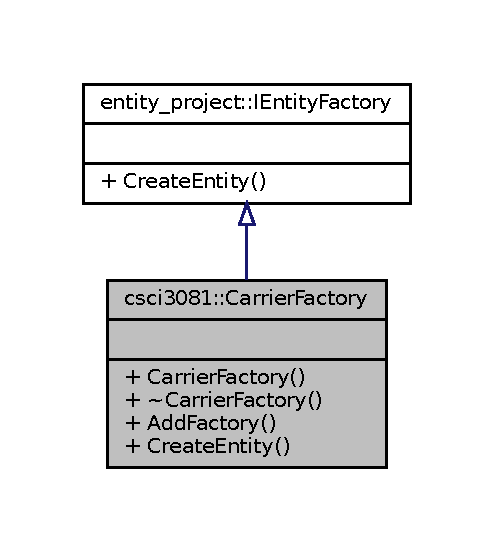
\includegraphics[width=237pt]{classcsci3081_1_1CarrierFactory__inherit__graph}
\end{center}
\end{figure}
\subsection*{Public Member Functions}
\begin{DoxyCompactItemize}
\item 
\mbox{\Hypertarget{classcsci3081_1_1CarrierFactory_a8de8128133312b8ccc3fc875072d81ca}\label{classcsci3081_1_1CarrierFactory_a8de8128133312b8ccc3fc875072d81ca}} 
\hyperlink{classcsci3081_1_1CarrierFactory_a8de8128133312b8ccc3fc875072d81ca}{Carrier\+Factory} ()
\begin{DoxyCompactList}\small\item\em Constructor\+: this can do any setup your system necessitates. \end{DoxyCompactList}\item 
\mbox{\Hypertarget{classcsci3081_1_1CarrierFactory_afeb21b32f748e85beaded1f1bc7e960a}\label{classcsci3081_1_1CarrierFactory_afeb21b32f748e85beaded1f1bc7e960a}} 
\hyperlink{classcsci3081_1_1CarrierFactory_afeb21b32f748e85beaded1f1bc7e960a}{$\sim$\+Carrier\+Factory} ()
\begin{DoxyCompactList}\small\item\em Destructor\+: this tear down/reset the memory space related to pointers. \end{DoxyCompactList}\item 
void \hyperlink{classcsci3081_1_1CarrierFactory_a83f8a2016ad118d028336b589262e3d2}{Add\+Factory} (\hyperlink{classentity__project_1_1IEntityFactory}{I\+Entity\+Factory} $\ast$)
\begin{DoxyCompactList}\small\item\em This adds an I\+Entity\+Factory factory into the vector factories of carrier class. \end{DoxyCompactList}\item 
\hyperlink{classentity__project_1_1IEntity}{I\+Entity} $\ast$ \hyperlink{classcsci3081_1_1CarrierFactory_a02cb728c8c3c6c8bf364998272ee1fa3}{Create\+Entity} (const picojson\+::object \&val)
\begin{DoxyCompactList}\small\item\em This is an inheritance function from I\+Entity\+Factory to create an approxiate Entity object based on the argument pass in Given the picojson\+::object val, this should create an entity. Based on the type of entity, there may be different fields. You can see the vals that will be passed in the project/web/scenes directory. Some of the fields are for our backend system and you don\textquotesingle{}t need to worry about them. (for instance, mesh, rotation, offset, etc.) Some fields in val that you will need to create the entity correctly\+: \end{DoxyCompactList}\end{DoxyCompactItemize}


\subsection{Detailed Description}
This is a derived class from I\+Entity\+Factory to manage all other factories (e.\+g. \hyperlink{classcsci3081_1_1DroneFactory}{Drone\+Factory}, \hyperlink{classcsci3081_1_1PackageFactory}{Package\+Factory}, \hyperlink{classcsci3081_1_1CustomerFactory}{Customer\+Factory}...) 

\subsection{Member Function Documentation}
\mbox{\Hypertarget{classcsci3081_1_1CarrierFactory_a83f8a2016ad118d028336b589262e3d2}\label{classcsci3081_1_1CarrierFactory_a83f8a2016ad118d028336b589262e3d2}} 
\index{csci3081\+::\+Carrier\+Factory@{csci3081\+::\+Carrier\+Factory}!Add\+Factory@{Add\+Factory}}
\index{Add\+Factory@{Add\+Factory}!csci3081\+::\+Carrier\+Factory@{csci3081\+::\+Carrier\+Factory}}
\subsubsection{\texorpdfstring{Add\+Factory()}{AddFactory()}}
{\footnotesize\ttfamily void csci3081\+::\+Carrier\+Factory\+::\+Add\+Factory (\begin{DoxyParamCaption}\item[{\hyperlink{classentity__project_1_1IEntityFactory}{I\+Entity\+Factory} $\ast$}]{n }\end{DoxyParamCaption})}



This adds an I\+Entity\+Factory factory into the vector factories of carrier class. 


\begin{DoxyParams}[1]{Parameters}
\mbox{\tt in}  & {\em n} & a I\+Entity\+Factory pointer that want to be added into the vector \\
\hline
\end{DoxyParams}
\mbox{\Hypertarget{classcsci3081_1_1CarrierFactory_a02cb728c8c3c6c8bf364998272ee1fa3}\label{classcsci3081_1_1CarrierFactory_a02cb728c8c3c6c8bf364998272ee1fa3}} 
\index{csci3081\+::\+Carrier\+Factory@{csci3081\+::\+Carrier\+Factory}!Create\+Entity@{Create\+Entity}}
\index{Create\+Entity@{Create\+Entity}!csci3081\+::\+Carrier\+Factory@{csci3081\+::\+Carrier\+Factory}}
\subsubsection{\texorpdfstring{Create\+Entity()}{CreateEntity()}}
{\footnotesize\ttfamily \hyperlink{classentity__project_1_1IEntity}{I\+Entity} $\ast$ csci3081\+::\+Carrier\+Factory\+::\+Create\+Entity (\begin{DoxyParamCaption}\item[{const picojson\+::object \&}]{val }\end{DoxyParamCaption})\hspace{0.3cm}{\ttfamily [virtual]}}



This is an inheritance function from I\+Entity\+Factory to create an approxiate Entity object based on the argument pass in Given the picojson\+::object val, this should create an entity. Based on the type of entity, there may be different fields. You can see the vals that will be passed in the project/web/scenes directory. Some of the fields are for our backend system and you don\textquotesingle{}t need to worry about them. (for instance, mesh, rotation, offset, etc.) Some fields in val that you will need to create the entity correctly\+: 

type\+: string (could be \char`\"{}drone/customer/package\char`\"{})

name\+: string

position\+: array (contains \mbox{[}x\+\_\+position, y\+\_\+position, z\+\_\+position\mbox{]})

direction\+: array (contains \mbox{[}x, y, z\mbox{]})

speed\+: float

battery\+\_\+capacity\+: float 
\begin{DoxyParams}[1]{Parameters}
\mbox{\tt in}  & {\em val} & the picojson\+::object that constains all of the necessary \\
\hline
\end{DoxyParams}
\begin{DoxyReturn}{Returns}
I\+Entity pointer information above in a json format 
\end{DoxyReturn}


Implements \hyperlink{classentity__project_1_1IEntityFactory_ac4e8eaf4294958fef0b98bd3684704bb}{entity\+\_\+project\+::\+I\+Entity\+Factory}.



The documentation for this class was generated from the following files\+:\begin{DoxyCompactItemize}
\item 
/home/user/repo/project/include/\hyperlink{carrier__factory_8h}{carrier\+\_\+factory.\+h}\item 
/home/user/repo/project/src/carrier\+\_\+factory.\+cc\end{DoxyCompactItemize}

\hypertarget{classcsci3081_1_1ChargingStation}{}\section{csci3081\+:\+:Charging\+Station Class Reference}
\label{classcsci3081_1_1ChargingStation}\index{csci3081\+::\+Charging\+Station@{csci3081\+::\+Charging\+Station}}


A representation of a \hyperlink{classcsci3081_1_1ChargingStation}{Charging\+Station}, inherited from \hyperlink{classcsci3081_1_1EntityBase}{Entity\+Base} It stores the \hyperlink{classcsci3081_1_1ChargingStation}{Charging\+Station}\textquotesingle{}s name, ID, version, position, direction, and dynamic mode.  




{\ttfamily \#include $<$charging\+\_\+station.\+h$>$}



Inheritance diagram for csci3081\+:\+:Charging\+Station\+:
\nopagebreak
\begin{figure}[H]
\begin{center}
\leavevmode
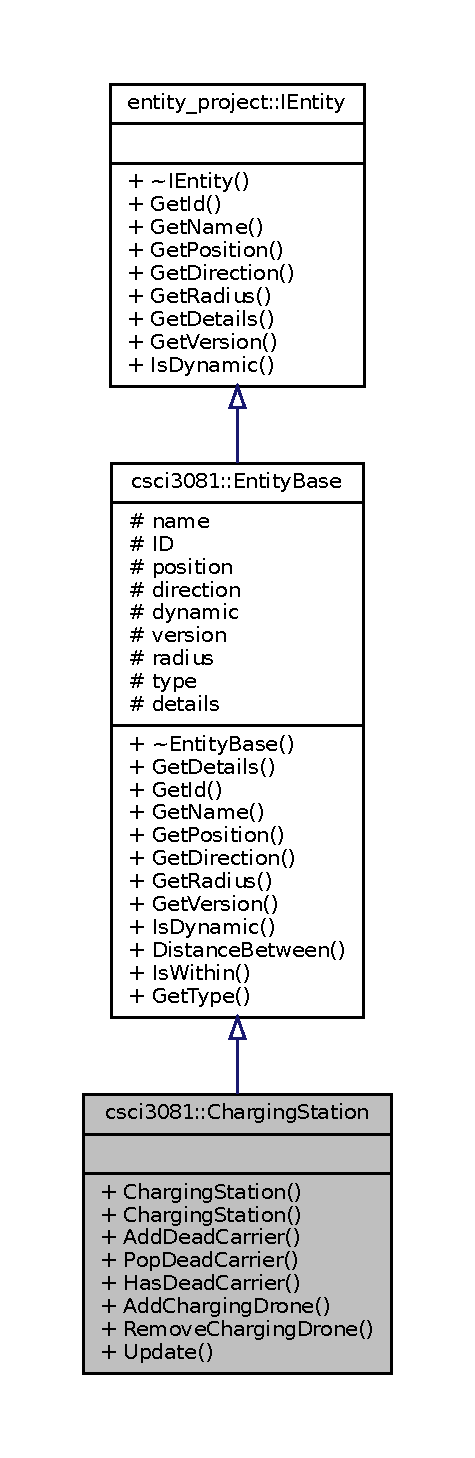
\includegraphics[height=550pt]{classcsci3081_1_1ChargingStation__inherit__graph}
\end{center}
\end{figure}
\subsection*{Public Member Functions}
\begin{DoxyCompactItemize}
\item 
\hyperlink{classcsci3081_1_1ChargingStation_a97fba4a68715e6b8305557c9b76571dd}{Charging\+Station} (const picojson\+::object \&val)
\item 
\hyperlink{classcsci3081_1_1ChargingStation_a3e5d04367a8cb19604714f6544e104b0}{Charging\+Station} (\hyperlink{classcsci3081_1_1ChargingStation}{Charging\+Station} \&charging\+Station)
\begin{DoxyCompactList}\small\item\em Copy Constructor. This creates a new instance of \hyperlink{classcsci3081_1_1ChargingStation}{Charging\+Station} that has the same content as the charging\+Station argument. \end{DoxyCompactList}\item 
void \hyperlink{classcsci3081_1_1ChargingStation_a903c7a2bf4e869ddae25409a567a16f2}{Add\+Dead\+Carrier} (\hyperlink{classcsci3081_1_1Carrier}{Carrier} $\ast$carrier)
\begin{DoxyCompactList}\small\item\em This adds a new dead carrier to a dead\+Carriers vector. \end{DoxyCompactList}\item 
\mbox{\Hypertarget{classcsci3081_1_1ChargingStation_a3c80d7f7982b2f14aff813fc0fa4772b}\label{classcsci3081_1_1ChargingStation_a3c80d7f7982b2f14aff813fc0fa4772b}} 
void \hyperlink{classcsci3081_1_1ChargingStation_a3c80d7f7982b2f14aff813fc0fa4772b}{Pop\+Dead\+Carrier} ()
\begin{DoxyCompactList}\small\item\em This removes the first dead carrier from a dead\+Carriers vector. This is due to a recharging drone that is heading towards a dead carrier to charge its battery. \end{DoxyCompactList}\item 
bool \hyperlink{classcsci3081_1_1ChargingStation_adb8fc616c40a8b8fd2b8e1259453ca9e}{Has\+Dead\+Carrier} (\hyperlink{classcsci3081_1_1Carrier}{Carrier} $\ast$carrier)
\begin{DoxyCompactList}\small\item\em This function checks if the charging station has already stored the dead carrier. \end{DoxyCompactList}\item 
bool \hyperlink{classcsci3081_1_1ChargingStation_a49703ccf92dd023e4be93b981d24904a}{Add\+Charging\+Drone} (\hyperlink{classcsci3081_1_1RechargeDrone}{Recharge\+Drone} $\ast$charging\+Drone)
\begin{DoxyCompactList}\small\item\em This adds a unique charging drone to the charging station only if the distance between the two is close together. \end{DoxyCompactList}\item 
void \hyperlink{classcsci3081_1_1ChargingStation_a10e78c7ca569a682b91498df6b5a9dd9}{Remove\+Charging\+Drone} (\hyperlink{classcsci3081_1_1RechargeDrone}{Recharge\+Drone} $\ast$charging\+Drone)
\begin{DoxyCompactList}\small\item\em This removes a charging drone from the charging station. This is due to a charging drone leaving the station to charge for a dead carrier. \end{DoxyCompactList}\item 
\mbox{\Hypertarget{classcsci3081_1_1ChargingStation_a1c07341a14013ac118f7bfbc88f2a597}\label{classcsci3081_1_1ChargingStation_a1c07341a14013ac118f7bfbc88f2a597}} 
void \hyperlink{classcsci3081_1_1ChargingStation_a1c07341a14013ac118f7bfbc88f2a597}{Update} (float dt)
\begin{DoxyCompactList}\small\item\em This is an inherited method from \hyperlink{classcsci3081_1_1EntityBase}{Entity\+Base} to use for \hyperlink{classcsci3081_1_1DeliverySimulation}{Delivery\+Simulation}. This updates the position of the carrier on the simulation if the position changes and its dynamic is set to true. In addition, this function also checks if the carrier is in within distance with the package to pick it up, or within distance with the customer to drop off the package. \end{DoxyCompactList}\end{DoxyCompactItemize}
\subsection*{Additional Inherited Members}


\subsection{Detailed Description}
A representation of a \hyperlink{classcsci3081_1_1ChargingStation}{Charging\+Station}, inherited from \hyperlink{classcsci3081_1_1EntityBase}{Entity\+Base} It stores the \hyperlink{classcsci3081_1_1ChargingStation}{Charging\+Station}\textquotesingle{}s name, ID, version, position, direction, and dynamic mode. 

\subsection{Constructor \& Destructor Documentation}
\mbox{\Hypertarget{classcsci3081_1_1ChargingStation_a97fba4a68715e6b8305557c9b76571dd}\label{classcsci3081_1_1ChargingStation_a97fba4a68715e6b8305557c9b76571dd}} 
\index{csci3081\+::\+Charging\+Station@{csci3081\+::\+Charging\+Station}!Charging\+Station@{Charging\+Station}}
\index{Charging\+Station@{Charging\+Station}!csci3081\+::\+Charging\+Station@{csci3081\+::\+Charging\+Station}}
\subsubsection{\texorpdfstring{Charging\+Station()}{ChargingStation()}\hspace{0.1cm}{\footnotesize\ttfamily [1/2]}}
{\footnotesize\ttfamily csci3081\+::\+Charging\+Station\+::\+Charging\+Station (\begin{DoxyParamCaption}\item[{const picojson\+::object \&}]{val }\end{DoxyParamCaption})}

Constructor param\mbox{[}in\mbox{]} val\+: the json object of the \hyperlink{classcsci3081_1_1ChargingStation}{Charging\+Station} \mbox{\Hypertarget{classcsci3081_1_1ChargingStation_a3e5d04367a8cb19604714f6544e104b0}\label{classcsci3081_1_1ChargingStation_a3e5d04367a8cb19604714f6544e104b0}} 
\index{csci3081\+::\+Charging\+Station@{csci3081\+::\+Charging\+Station}!Charging\+Station@{Charging\+Station}}
\index{Charging\+Station@{Charging\+Station}!csci3081\+::\+Charging\+Station@{csci3081\+::\+Charging\+Station}}
\subsubsection{\texorpdfstring{Charging\+Station()}{ChargingStation()}\hspace{0.1cm}{\footnotesize\ttfamily [2/2]}}
{\footnotesize\ttfamily csci3081\+::\+Charging\+Station\+::\+Charging\+Station (\begin{DoxyParamCaption}\item[{\hyperlink{classcsci3081_1_1ChargingStation}{Charging\+Station} \&}]{charging\+Station }\end{DoxyParamCaption})}



Copy Constructor. This creates a new instance of \hyperlink{classcsci3081_1_1ChargingStation}{Charging\+Station} that has the same content as the charging\+Station argument. 


\begin{DoxyParams}[1]{Parameters}
\mbox{\tt in}  & {\em charging\+Station} & charging\+Station instance that wants to be copied \\
\hline
\end{DoxyParams}


\subsection{Member Function Documentation}
\mbox{\Hypertarget{classcsci3081_1_1ChargingStation_a49703ccf92dd023e4be93b981d24904a}\label{classcsci3081_1_1ChargingStation_a49703ccf92dd023e4be93b981d24904a}} 
\index{csci3081\+::\+Charging\+Station@{csci3081\+::\+Charging\+Station}!Add\+Charging\+Drone@{Add\+Charging\+Drone}}
\index{Add\+Charging\+Drone@{Add\+Charging\+Drone}!csci3081\+::\+Charging\+Station@{csci3081\+::\+Charging\+Station}}
\subsubsection{\texorpdfstring{Add\+Charging\+Drone()}{AddChargingDrone()}}
{\footnotesize\ttfamily bool csci3081\+::\+Charging\+Station\+::\+Add\+Charging\+Drone (\begin{DoxyParamCaption}\item[{\hyperlink{classcsci3081_1_1RechargeDrone}{Recharge\+Drone} $\ast$}]{charging\+Drone }\end{DoxyParamCaption})}



This adds a unique charging drone to the charging station only if the distance between the two is close together. 


\begin{DoxyParams}[1]{Parameters}
\mbox{\tt in}  & {\em charging\+Drone} & A charging drone to be added to the charging station. \\
\hline
\end{DoxyParams}
\begin{DoxyReturn}{Returns}
bool Returns true if the charging drone was successfully added. False otherwise. 
\end{DoxyReturn}
\mbox{\Hypertarget{classcsci3081_1_1ChargingStation_a903c7a2bf4e869ddae25409a567a16f2}\label{classcsci3081_1_1ChargingStation_a903c7a2bf4e869ddae25409a567a16f2}} 
\index{csci3081\+::\+Charging\+Station@{csci3081\+::\+Charging\+Station}!Add\+Dead\+Carrier@{Add\+Dead\+Carrier}}
\index{Add\+Dead\+Carrier@{Add\+Dead\+Carrier}!csci3081\+::\+Charging\+Station@{csci3081\+::\+Charging\+Station}}
\subsubsection{\texorpdfstring{Add\+Dead\+Carrier()}{AddDeadCarrier()}}
{\footnotesize\ttfamily void csci3081\+::\+Charging\+Station\+::\+Add\+Dead\+Carrier (\begin{DoxyParamCaption}\item[{\hyperlink{classcsci3081_1_1Carrier}{Carrier} $\ast$}]{carrier }\end{DoxyParamCaption})}



This adds a new dead carrier to a dead\+Carriers vector. 


\begin{DoxyParams}[1]{Parameters}
\mbox{\tt in}  & {\em carrier} & A new carrier to be added to dead\+Carriers vector. \\
\hline
\end{DoxyParams}
\mbox{\Hypertarget{classcsci3081_1_1ChargingStation_adb8fc616c40a8b8fd2b8e1259453ca9e}\label{classcsci3081_1_1ChargingStation_adb8fc616c40a8b8fd2b8e1259453ca9e}} 
\index{csci3081\+::\+Charging\+Station@{csci3081\+::\+Charging\+Station}!Has\+Dead\+Carrier@{Has\+Dead\+Carrier}}
\index{Has\+Dead\+Carrier@{Has\+Dead\+Carrier}!csci3081\+::\+Charging\+Station@{csci3081\+::\+Charging\+Station}}
\subsubsection{\texorpdfstring{Has\+Dead\+Carrier()}{HasDeadCarrier()}}
{\footnotesize\ttfamily bool csci3081\+::\+Charging\+Station\+::\+Has\+Dead\+Carrier (\begin{DoxyParamCaption}\item[{\hyperlink{classcsci3081_1_1Carrier}{Carrier} $\ast$}]{carrier }\end{DoxyParamCaption})}



This function checks if the charging station has already stored the dead carrier. 


\begin{DoxyParams}[1]{Parameters}
\mbox{\tt in}  & {\em carrier} & Dead carrier to be checked if noted in the charging station \\
\hline
\end{DoxyParams}
\begin{DoxyReturn}{Returns}
bool True if the charging station has already stored the dead carrier. False otherwise. 
\end{DoxyReturn}
\mbox{\Hypertarget{classcsci3081_1_1ChargingStation_a10e78c7ca569a682b91498df6b5a9dd9}\label{classcsci3081_1_1ChargingStation_a10e78c7ca569a682b91498df6b5a9dd9}} 
\index{csci3081\+::\+Charging\+Station@{csci3081\+::\+Charging\+Station}!Remove\+Charging\+Drone@{Remove\+Charging\+Drone}}
\index{Remove\+Charging\+Drone@{Remove\+Charging\+Drone}!csci3081\+::\+Charging\+Station@{csci3081\+::\+Charging\+Station}}
\subsubsection{\texorpdfstring{Remove\+Charging\+Drone()}{RemoveChargingDrone()}}
{\footnotesize\ttfamily void csci3081\+::\+Charging\+Station\+::\+Remove\+Charging\+Drone (\begin{DoxyParamCaption}\item[{\hyperlink{classcsci3081_1_1RechargeDrone}{Recharge\+Drone} $\ast$}]{charging\+Drone }\end{DoxyParamCaption})}



This removes a charging drone from the charging station. This is due to a charging drone leaving the station to charge for a dead carrier. 


\begin{DoxyParams}[1]{Parameters}
\mbox{\tt in}  & {\em charging\+Drone} & A charging drone to be removed from the charging station. \\
\hline
\end{DoxyParams}


The documentation for this class was generated from the following files\+:\begin{DoxyCompactItemize}
\item 
/home/user/repo/project/include/\hyperlink{charging__station_8h}{charging\+\_\+station.\+h}\item 
/home/user/repo/project/src/charging\+\_\+station.\+cc\end{DoxyCompactItemize}

\hypertarget{classcsci3081_1_1ChargingStationFactory}{}\section{csci3081\+:\+:Charging\+Station\+Factory Class Reference}
\label{classcsci3081_1_1ChargingStationFactory}\index{csci3081\+::\+Charging\+Station\+Factory@{csci3081\+::\+Charging\+Station\+Factory}}


This is the \hyperlink{classcsci3081_1_1ChargingStationFactory}{Charging\+Station\+Factory}, responsible for making charging station object.  




{\ttfamily \#include $<$charging\+\_\+station\+\_\+factory.\+h$>$}



Inheritance diagram for csci3081\+:\+:Charging\+Station\+Factory\+:
\nopagebreak
\begin{figure}[H]
\begin{center}
\leavevmode
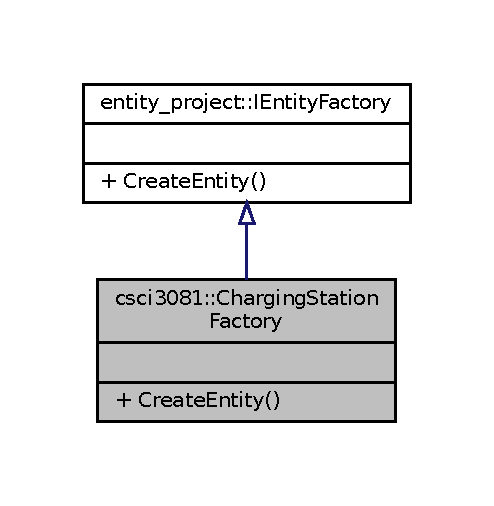
\includegraphics[width=237pt]{classcsci3081_1_1ChargingStationFactory__inherit__graph}
\end{center}
\end{figure}
\subsection*{Public Member Functions}
\begin{DoxyCompactItemize}
\item 
\hyperlink{classentity__project_1_1IEntity}{I\+Entity} $\ast$ \hyperlink{classcsci3081_1_1ChargingStationFactory_ad7099c9c36583ea8f608cef89200c8e9}{Create\+Entity} (const picojson\+::object \&val)
\begin{DoxyCompactList}\small\item\em This is an inheritance function from I\+Entity\+Factory to create an approxiate Entity object based on the argument pass in Given the picojson\+::object val, this should create an entity. Based on the type of entity, there may be different fields. You can see the vals that will be passed in the project/web/scenes directory. Some of the fields are for our backend system and you don\textquotesingle{}t need to worry about them. (for instance, mesh, rotation, offset, etc.) Some fields in val that you will need to create the entity correctly\+: \end{DoxyCompactList}\end{DoxyCompactItemize}


\subsection{Detailed Description}
This is the \hyperlink{classcsci3081_1_1ChargingStationFactory}{Charging\+Station\+Factory}, responsible for making charging station object. 

\subsection{Member Function Documentation}
\mbox{\Hypertarget{classcsci3081_1_1ChargingStationFactory_ad7099c9c36583ea8f608cef89200c8e9}\label{classcsci3081_1_1ChargingStationFactory_ad7099c9c36583ea8f608cef89200c8e9}} 
\index{csci3081\+::\+Charging\+Station\+Factory@{csci3081\+::\+Charging\+Station\+Factory}!Create\+Entity@{Create\+Entity}}
\index{Create\+Entity@{Create\+Entity}!csci3081\+::\+Charging\+Station\+Factory@{csci3081\+::\+Charging\+Station\+Factory}}
\subsubsection{\texorpdfstring{Create\+Entity()}{CreateEntity()}}
{\footnotesize\ttfamily \hyperlink{classentity__project_1_1IEntity}{I\+Entity} $\ast$ csci3081\+::\+Charging\+Station\+Factory\+::\+Create\+Entity (\begin{DoxyParamCaption}\item[{const picojson\+::object \&}]{val }\end{DoxyParamCaption})\hspace{0.3cm}{\ttfamily [virtual]}}



This is an inheritance function from I\+Entity\+Factory to create an approxiate Entity object based on the argument pass in Given the picojson\+::object val, this should create an entity. Based on the type of entity, there may be different fields. You can see the vals that will be passed in the project/web/scenes directory. Some of the fields are for our backend system and you don\textquotesingle{}t need to worry about them. (for instance, mesh, rotation, offset, etc.) Some fields in val that you will need to create the entity correctly\+: 

type\+: string (could be \char`\"{}drone/customer/package\char`\"{})

name\+: string

position\+: array (contains \mbox{[}x\+\_\+position, y\+\_\+position, z\+\_\+position\mbox{]})

direction\+: array (contains \mbox{[}x, y, z\mbox{]})


\begin{DoxyParams}[1]{Parameters}
\mbox{\tt in}  & {\em val} & the picojson\+::object that constains all of the necessary information above in a json format \\
\hline
\end{DoxyParams}
\begin{DoxyReturn}{Returns}
I\+Entity pointer if the object has type \char`\"{}customer\char`\"{}; N\+U\+LL otherwise 
\end{DoxyReturn}


Implements \hyperlink{classentity__project_1_1IEntityFactory_ac4e8eaf4294958fef0b98bd3684704bb}{entity\+\_\+project\+::\+I\+Entity\+Factory}.



The documentation for this class was generated from the following files\+:\begin{DoxyCompactItemize}
\item 
/home/user/repo/project/include/\hyperlink{charging__station__factory_8h}{charging\+\_\+station\+\_\+factory.\+h}\item 
/home/user/repo/project/src/charging\+\_\+station\+\_\+factory.\+cc\end{DoxyCompactItemize}

\hypertarget{classcsci3081_1_1CompositeFactory}{}\section{csci3081\+:\+:Composite\+Factory Class Reference}
\label{classcsci3081_1_1CompositeFactory}\index{csci3081\+::\+Composite\+Factory@{csci3081\+::\+Composite\+Factory}}


This is a derived class from I\+Entity\+Factory to manage all other factories (e.\+g. \hyperlink{classcsci3081_1_1DroneFactory}{Drone\+Factory}, \hyperlink{classcsci3081_1_1PackageFactory}{Package\+Factory}, \hyperlink{classcsci3081_1_1CustomerFactory}{Customer\+Factory}...)  




{\ttfamily \#include $<$composite\+\_\+factory.\+h$>$}



Inheritance diagram for csci3081\+:\+:Composite\+Factory\+:
\nopagebreak
\begin{figure}[H]
\begin{center}
\leavevmode
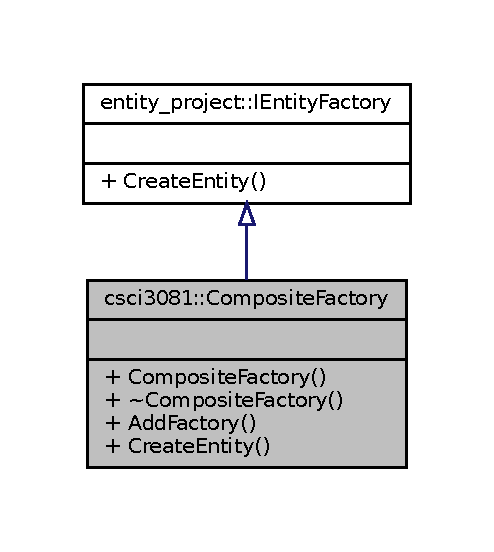
\includegraphics[width=237pt]{classcsci3081_1_1CompositeFactory__inherit__graph}
\end{center}
\end{figure}
\subsection*{Public Member Functions}
\begin{DoxyCompactItemize}
\item 
\mbox{\Hypertarget{classcsci3081_1_1CompositeFactory_a4f7bb7bd2003311b131b2c346d0dc02e}\label{classcsci3081_1_1CompositeFactory_a4f7bb7bd2003311b131b2c346d0dc02e}} 
\hyperlink{classcsci3081_1_1CompositeFactory_a4f7bb7bd2003311b131b2c346d0dc02e}{Composite\+Factory} ()
\begin{DoxyCompactList}\small\item\em Constructor\+: this can do any setup your system necessitates. \end{DoxyCompactList}\item 
\mbox{\Hypertarget{classcsci3081_1_1CompositeFactory_a6b29e079c772c7068e6fe789f0298297}\label{classcsci3081_1_1CompositeFactory_a6b29e079c772c7068e6fe789f0298297}} 
\hyperlink{classcsci3081_1_1CompositeFactory_a6b29e079c772c7068e6fe789f0298297}{$\sim$\+Composite\+Factory} ()
\begin{DoxyCompactList}\small\item\em Destructor\+: this tear down/reset the memory space related to pointers. \end{DoxyCompactList}\item 
void \hyperlink{classcsci3081_1_1CompositeFactory_a3aa41268f20303f8e6f5e2a1d2422e0a}{Add\+Factory} (\hyperlink{classentity__project_1_1IEntityFactory}{I\+Entity\+Factory} $\ast$)
\begin{DoxyCompactList}\small\item\em This adds an I\+Entity\+Factory factory into the vector factories of composite class. \end{DoxyCompactList}\item 
\hyperlink{classentity__project_1_1IEntity}{I\+Entity} $\ast$ \hyperlink{classcsci3081_1_1CompositeFactory_a2933003742d1660515c009ec04b8d5b4}{Create\+Entity} (const picojson\+::object \&val)
\begin{DoxyCompactList}\small\item\em This is an inheritance function from I\+Entity\+Factory to create an approxiate Entity object based on the argument pass in Given the picojson\+::object val, this should create an entity. Based on the type of entity, there may be different fields. You can see the vals that will be passed in the project/web/scenes directory. Some of the fields are for our backend system and you don\textquotesingle{}t need to worry about them. (for instance, mesh, rotation, offset, etc.) Some fields in val that you will need to create the entity correctly\+: \end{DoxyCompactList}\end{DoxyCompactItemize}


\subsection{Detailed Description}
This is a derived class from I\+Entity\+Factory to manage all other factories (e.\+g. \hyperlink{classcsci3081_1_1DroneFactory}{Drone\+Factory}, \hyperlink{classcsci3081_1_1PackageFactory}{Package\+Factory}, \hyperlink{classcsci3081_1_1CustomerFactory}{Customer\+Factory}...) 

\subsection{Member Function Documentation}
\mbox{\Hypertarget{classcsci3081_1_1CompositeFactory_a3aa41268f20303f8e6f5e2a1d2422e0a}\label{classcsci3081_1_1CompositeFactory_a3aa41268f20303f8e6f5e2a1d2422e0a}} 
\index{csci3081\+::\+Composite\+Factory@{csci3081\+::\+Composite\+Factory}!Add\+Factory@{Add\+Factory}}
\index{Add\+Factory@{Add\+Factory}!csci3081\+::\+Composite\+Factory@{csci3081\+::\+Composite\+Factory}}
\subsubsection{\texorpdfstring{Add\+Factory()}{AddFactory()}}
{\footnotesize\ttfamily void csci3081\+::\+Composite\+Factory\+::\+Add\+Factory (\begin{DoxyParamCaption}\item[{\hyperlink{classentity__project_1_1IEntityFactory}{I\+Entity\+Factory} $\ast$}]{n }\end{DoxyParamCaption})}



This adds an I\+Entity\+Factory factory into the vector factories of composite class. 


\begin{DoxyParams}[1]{Parameters}
\mbox{\tt in}  & {\em n} & a I\+Entity\+Factory pointer that want to be added into the vector \\
\hline
\end{DoxyParams}
\mbox{\Hypertarget{classcsci3081_1_1CompositeFactory_a2933003742d1660515c009ec04b8d5b4}\label{classcsci3081_1_1CompositeFactory_a2933003742d1660515c009ec04b8d5b4}} 
\index{csci3081\+::\+Composite\+Factory@{csci3081\+::\+Composite\+Factory}!Create\+Entity@{Create\+Entity}}
\index{Create\+Entity@{Create\+Entity}!csci3081\+::\+Composite\+Factory@{csci3081\+::\+Composite\+Factory}}
\subsubsection{\texorpdfstring{Create\+Entity()}{CreateEntity()}}
{\footnotesize\ttfamily \hyperlink{classentity__project_1_1IEntity}{I\+Entity} $\ast$ csci3081\+::\+Composite\+Factory\+::\+Create\+Entity (\begin{DoxyParamCaption}\item[{const picojson\+::object \&}]{val }\end{DoxyParamCaption})\hspace{0.3cm}{\ttfamily [virtual]}}



This is an inheritance function from I\+Entity\+Factory to create an approxiate Entity object based on the argument pass in Given the picojson\+::object val, this should create an entity. Based on the type of entity, there may be different fields. You can see the vals that will be passed in the project/web/scenes directory. Some of the fields are for our backend system and you don\textquotesingle{}t need to worry about them. (for instance, mesh, rotation, offset, etc.) Some fields in val that you will need to create the entity correctly\+: 

type\+: string (could be \char`\"{}drone/customer/package\char`\"{})

name\+: string

position\+: array (contains \mbox{[}x\+\_\+position, y\+\_\+position, z\+\_\+position\mbox{]})

direction\+: array (contains \mbox{[}x, y, z\mbox{]})

speed\+: float

battery\+\_\+capacity\+: float 
\begin{DoxyParams}[1]{Parameters}
\mbox{\tt in}  & {\em val} & the picojson\+::object that constains all of the necessary \\
\hline
\end{DoxyParams}
\begin{DoxyReturn}{Returns}
I\+Entity pointer information above in a json format 
\end{DoxyReturn}


Implements \hyperlink{classentity__project_1_1IEntityFactory_ac4e8eaf4294958fef0b98bd3684704bb}{entity\+\_\+project\+::\+I\+Entity\+Factory}.



The documentation for this class was generated from the following files\+:\begin{DoxyCompactItemize}
\item 
/home/user/repo/project/include/\hyperlink{composite__factory_8h}{composite\+\_\+factory.\+h}\item 
/home/user/repo/project/src/composite\+\_\+factory.\+cc\end{DoxyCompactItemize}

\hypertarget{classcsci3081_1_1Customer}{}\section{csci3081\+:\+:Customer Class Reference}
\label{classcsci3081_1_1Customer}\index{csci3081\+::\+Customer@{csci3081\+::\+Customer}}


A representation of a \hyperlink{classcsci3081_1_1Customer}{Customer}, inherited from \hyperlink{classcsci3081_1_1EntityBase}{Entity\+Base} It stores the \hyperlink{classcsci3081_1_1Customer}{Customer}\textquotesingle{}s name, ID, version, position, direction, and dynamic mode.  




{\ttfamily \#include $<$customer.\+h$>$}



Inheritance diagram for csci3081\+:\+:Customer\+:
\nopagebreak
\begin{figure}[H]
\begin{center}
\leavevmode
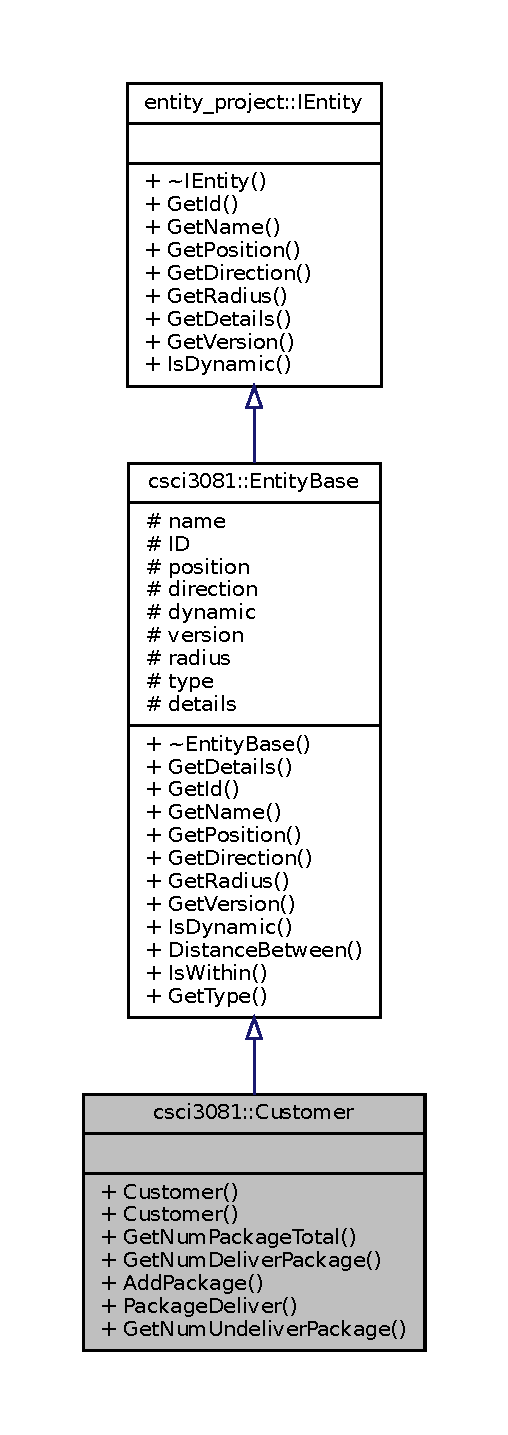
\includegraphics[height=550pt]{classcsci3081_1_1Customer__inherit__graph}
\end{center}
\end{figure}
\subsection*{Public Member Functions}
\begin{DoxyCompactItemize}
\item 
\hyperlink{classcsci3081_1_1Customer_abbbf2b0f11d653b3cb0c2926064a830a}{Customer} (const picojson\+::object \&val)
\item 
\hyperlink{classcsci3081_1_1Customer_ad4eec3e1ba0f5dbe815e8552eb1715e2}{Customer} (\hyperlink{classcsci3081_1_1Customer}{Customer} \&customer)
\begin{DoxyCompactList}\small\item\em Copy Constructor. This creates a new instance of \hyperlink{classcsci3081_1_1Customer}{Customer} that has the same content as the \hyperlink{classcsci3081_1_1Customer}{Customer} argument. \end{DoxyCompactList}\item 
\mbox{\Hypertarget{classcsci3081_1_1Customer_a9547aa6dd6c208f56ca02f945bd9441e}\label{classcsci3081_1_1Customer_a9547aa6dd6c208f56ca02f945bd9441e}} 
int \hyperlink{classcsci3081_1_1Customer_a9547aa6dd6c208f56ca02f945bd9441e}{Get\+Num\+Package\+Total} () const
\begin{DoxyCompactList}\small\item\em This return the number of packages the customer has in total. \end{DoxyCompactList}\item 
\mbox{\Hypertarget{classcsci3081_1_1Customer_a1f6ddb2ecac6de13f8e5631483b959ea}\label{classcsci3081_1_1Customer_a1f6ddb2ecac6de13f8e5631483b959ea}} 
int \hyperlink{classcsci3081_1_1Customer_a1f6ddb2ecac6de13f8e5631483b959ea}{Get\+Num\+Deliver\+Package} () const
\begin{DoxyCompactList}\small\item\em This return the number of packages the customer has in total. \end{DoxyCompactList}\item 
void \hyperlink{classcsci3081_1_1Customer_a7eba42384d9648731c81862c36fed1ec}{Add\+Package} (int package\+ID)
\begin{DoxyCompactList}\small\item\em This adds a package ID into the customer\textquotesingle{}s tracked package\+ID vector if the package has not already been added. This would help check package delivery for the customer. \end{DoxyCompactList}\item 
bool \hyperlink{classcsci3081_1_1Customer_a0277fdbb1cdb28f8932f69ead7eadf9f}{Package\+Deliver} (int package\+ID)
\begin{DoxyCompactList}\small\item\em This returns T\+R\+UE if the package with the ID passed in has already been delivered; F\+A\+L\+SE otherwise. \end{DoxyCompactList}\item 
\mbox{\Hypertarget{classcsci3081_1_1Customer_a82be2bf29df5167f5f6e15c510597bf7}\label{classcsci3081_1_1Customer_a82be2bf29df5167f5f6e15c510597bf7}} 
int \hyperlink{classcsci3081_1_1Customer_a82be2bf29df5167f5f6e15c510597bf7}{Get\+Num\+Undeliver\+Package} () const
\begin{DoxyCompactList}\small\item\em This return the number of undelivered packages the customer has. \end{DoxyCompactList}\end{DoxyCompactItemize}
\subsection*{Additional Inherited Members}


\subsection{Detailed Description}
A representation of a \hyperlink{classcsci3081_1_1Customer}{Customer}, inherited from \hyperlink{classcsci3081_1_1EntityBase}{Entity\+Base} It stores the \hyperlink{classcsci3081_1_1Customer}{Customer}\textquotesingle{}s name, ID, version, position, direction, and dynamic mode. 

\subsection{Constructor \& Destructor Documentation}
\mbox{\Hypertarget{classcsci3081_1_1Customer_abbbf2b0f11d653b3cb0c2926064a830a}\label{classcsci3081_1_1Customer_abbbf2b0f11d653b3cb0c2926064a830a}} 
\index{csci3081\+::\+Customer@{csci3081\+::\+Customer}!Customer@{Customer}}
\index{Customer@{Customer}!csci3081\+::\+Customer@{csci3081\+::\+Customer}}
\subsubsection{\texorpdfstring{Customer()}{Customer()}\hspace{0.1cm}{\footnotesize\ttfamily [1/2]}}
{\footnotesize\ttfamily csci3081\+::\+Customer\+::\+Customer (\begin{DoxyParamCaption}\item[{const picojson\+::object \&}]{val }\end{DoxyParamCaption})}

Constructor param\mbox{[}in\mbox{]} val\+: the json object of the \hyperlink{classcsci3081_1_1Customer}{Customer} \mbox{\Hypertarget{classcsci3081_1_1Customer_ad4eec3e1ba0f5dbe815e8552eb1715e2}\label{classcsci3081_1_1Customer_ad4eec3e1ba0f5dbe815e8552eb1715e2}} 
\index{csci3081\+::\+Customer@{csci3081\+::\+Customer}!Customer@{Customer}}
\index{Customer@{Customer}!csci3081\+::\+Customer@{csci3081\+::\+Customer}}
\subsubsection{\texorpdfstring{Customer()}{Customer()}\hspace{0.1cm}{\footnotesize\ttfamily [2/2]}}
{\footnotesize\ttfamily csci3081\+::\+Customer\+::\+Customer (\begin{DoxyParamCaption}\item[{\hyperlink{classcsci3081_1_1Customer}{Customer} \&}]{customer }\end{DoxyParamCaption})}



Copy Constructor. This creates a new instance of \hyperlink{classcsci3081_1_1Customer}{Customer} that has the same content as the \hyperlink{classcsci3081_1_1Customer}{Customer} argument. 


\begin{DoxyParams}[1]{Parameters}
\mbox{\tt in}  & {\em customer} & \hyperlink{classcsci3081_1_1Customer}{Customer} instance that wants to be copied \\
\hline
\end{DoxyParams}


\subsection{Member Function Documentation}
\mbox{\Hypertarget{classcsci3081_1_1Customer_a7eba42384d9648731c81862c36fed1ec}\label{classcsci3081_1_1Customer_a7eba42384d9648731c81862c36fed1ec}} 
\index{csci3081\+::\+Customer@{csci3081\+::\+Customer}!Add\+Package@{Add\+Package}}
\index{Add\+Package@{Add\+Package}!csci3081\+::\+Customer@{csci3081\+::\+Customer}}
\subsubsection{\texorpdfstring{Add\+Package()}{AddPackage()}}
{\footnotesize\ttfamily void csci3081\+::\+Customer\+::\+Add\+Package (\begin{DoxyParamCaption}\item[{int}]{package\+ID }\end{DoxyParamCaption})}



This adds a package ID into the customer\textquotesingle{}s tracked package\+ID vector if the package has not already been added. This would help check package delivery for the customer. 


\begin{DoxyParams}[1]{Parameters}
\mbox{\tt in}  & {\em package\+ID} & the int for the ID of the package \\
\hline
\end{DoxyParams}
\mbox{\Hypertarget{classcsci3081_1_1Customer_a0277fdbb1cdb28f8932f69ead7eadf9f}\label{classcsci3081_1_1Customer_a0277fdbb1cdb28f8932f69ead7eadf9f}} 
\index{csci3081\+::\+Customer@{csci3081\+::\+Customer}!Package\+Deliver@{Package\+Deliver}}
\index{Package\+Deliver@{Package\+Deliver}!csci3081\+::\+Customer@{csci3081\+::\+Customer}}
\subsubsection{\texorpdfstring{Package\+Deliver()}{PackageDeliver()}}
{\footnotesize\ttfamily bool csci3081\+::\+Customer\+::\+Package\+Deliver (\begin{DoxyParamCaption}\item[{int}]{package\+ID }\end{DoxyParamCaption})}



This returns T\+R\+UE if the package with the ID passed in has already been delivered; F\+A\+L\+SE otherwise. 


\begin{DoxyParams}[1]{Parameters}
\mbox{\tt in}  & {\em package\+ID} & the int for the ID of the package \\
\hline
\end{DoxyParams}


The documentation for this class was generated from the following files\+:\begin{DoxyCompactItemize}
\item 
/home/user/repo/project/include/customer.\+h\item 
/home/user/repo/project/src/customer.\+cc\end{DoxyCompactItemize}

\hypertarget{classcsci3081_1_1CustomerFactory}{}\section{csci3081\+:\+:Customer\+Factory Class Reference}
\label{classcsci3081_1_1CustomerFactory}\index{csci3081\+::\+Customer\+Factory@{csci3081\+::\+Customer\+Factory}}


This is the \hyperlink{classcsci3081_1_1CustomerFactory}{Customer\+Factory}, responsible for making \hyperlink{classcsci3081_1_1Customer}{Customer} object.  




{\ttfamily \#include $<$customer\+\_\+factory.\+h$>$}



Inheritance diagram for csci3081\+:\+:Customer\+Factory\+:
\nopagebreak
\begin{figure}[H]
\begin{center}
\leavevmode
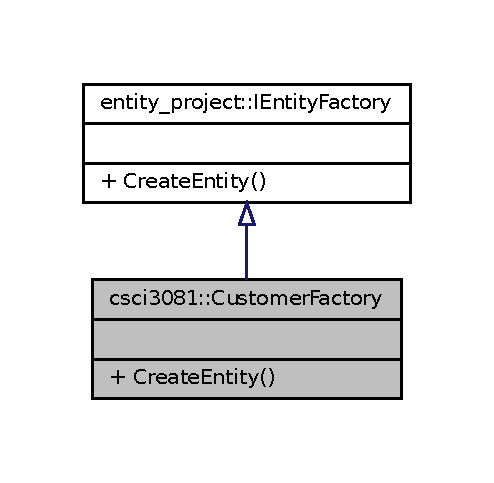
\includegraphics[width=237pt]{classcsci3081_1_1CustomerFactory__inherit__graph}
\end{center}
\end{figure}
\subsection*{Public Member Functions}
\begin{DoxyCompactItemize}
\item 
\hyperlink{classentity__project_1_1IEntity}{I\+Entity} $\ast$ \hyperlink{classcsci3081_1_1CustomerFactory_ad184f214fa10ad531e1ae2432142fc45}{Create\+Entity} (const picojson\+::object \&val)
\begin{DoxyCompactList}\small\item\em This is an inheritance function from I\+Entity\+Factory to create an approxiate Entity object based on the argument pass in Given the picojson\+::object val, this should create an entity. Based on the type of entity, there may be different fields. You can see the vals that will be passed in the project/web/scenes directory. Some of the fields are for our backend system and you don\textquotesingle{}t need to worry about them. (for instance, mesh, rotation, offset, etc.) Some fields in val that you will need to create the entity correctly\+: \end{DoxyCompactList}\end{DoxyCompactItemize}


\subsection{Detailed Description}
This is the \hyperlink{classcsci3081_1_1CustomerFactory}{Customer\+Factory}, responsible for making \hyperlink{classcsci3081_1_1Customer}{Customer} object. 

\subsection{Member Function Documentation}
\mbox{\Hypertarget{classcsci3081_1_1CustomerFactory_ad184f214fa10ad531e1ae2432142fc45}\label{classcsci3081_1_1CustomerFactory_ad184f214fa10ad531e1ae2432142fc45}} 
\index{csci3081\+::\+Customer\+Factory@{csci3081\+::\+Customer\+Factory}!Create\+Entity@{Create\+Entity}}
\index{Create\+Entity@{Create\+Entity}!csci3081\+::\+Customer\+Factory@{csci3081\+::\+Customer\+Factory}}
\subsubsection{\texorpdfstring{Create\+Entity()}{CreateEntity()}}
{\footnotesize\ttfamily \hyperlink{classentity__project_1_1IEntity}{I\+Entity} $\ast$ csci3081\+::\+Customer\+Factory\+::\+Create\+Entity (\begin{DoxyParamCaption}\item[{const picojson\+::object \&}]{val }\end{DoxyParamCaption})\hspace{0.3cm}{\ttfamily [virtual]}}



This is an inheritance function from I\+Entity\+Factory to create an approxiate Entity object based on the argument pass in Given the picojson\+::object val, this should create an entity. Based on the type of entity, there may be different fields. You can see the vals that will be passed in the project/web/scenes directory. Some of the fields are for our backend system and you don\textquotesingle{}t need to worry about them. (for instance, mesh, rotation, offset, etc.) Some fields in val that you will need to create the entity correctly\+: 

type\+: string (could be \char`\"{}drone/customer/package\char`\"{})

name\+: string

position\+: array (contains \mbox{[}x\+\_\+position, y\+\_\+position, z\+\_\+position\mbox{]})

direction\+: array (contains \mbox{[}x, y, z\mbox{]})


\begin{DoxyParams}[1]{Parameters}
\mbox{\tt in}  & {\em val} & the picojson\+::object that constains all of the necessary information above in a json format \\
\hline
\end{DoxyParams}
\begin{DoxyReturn}{Returns}
I\+Entity pointer if the object has type \char`\"{}customer\char`\"{}; N\+U\+LL otherwise 
\end{DoxyReturn}


Implements \hyperlink{classentity__project_1_1IEntityFactory_ac4e8eaf4294958fef0b98bd3684704bb}{entity\+\_\+project\+::\+I\+Entity\+Factory}.



The documentation for this class was generated from the following files\+:\begin{DoxyCompactItemize}
\item 
/home/user/repo/project/include/customer\+\_\+factory.\+h\item 
/home/user/repo/project/src/customer\+\_\+factory.\+cc\end{DoxyCompactItemize}

\hypertarget{classcsci3081_1_1DeliverySimulation}{}\section{csci3081\+:\+:Delivery\+Simulation Class Reference}
\label{classcsci3081_1_1DeliverySimulation}\index{csci3081\+::\+Delivery\+Simulation@{csci3081\+::\+Delivery\+Simulation}}


This is the facade for the delivery system.  




{\ttfamily \#include $<$delivery\+\_\+simulation.\+h$>$}



Inheritance diagram for csci3081\+:\+:Delivery\+Simulation\+:
\nopagebreak
\begin{figure}[H]
\begin{center}
\leavevmode
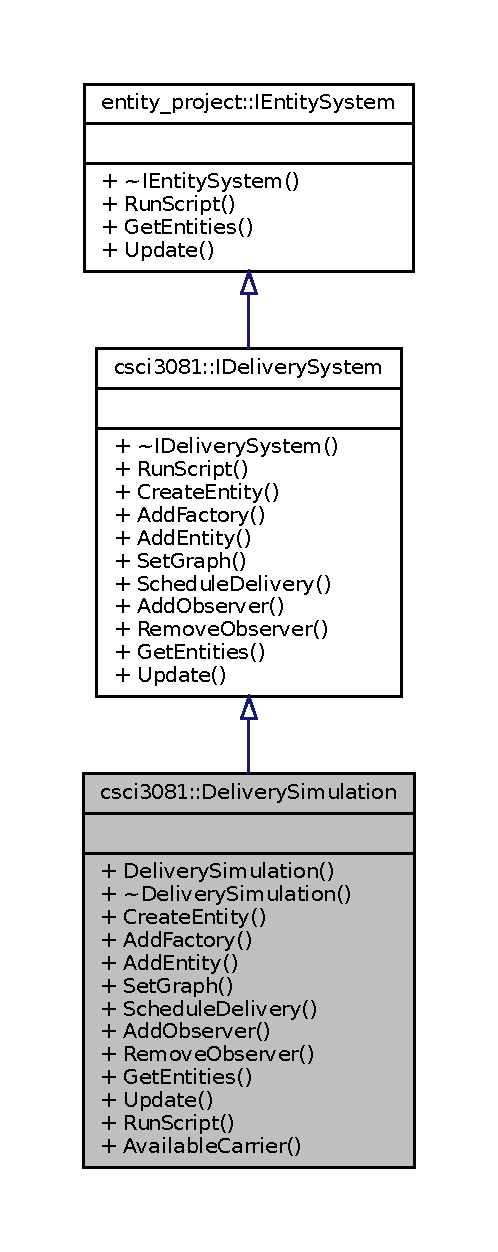
\includegraphics[height=550pt]{classcsci3081_1_1DeliverySimulation__inherit__graph}
\end{center}
\end{figure}
\subsection*{Public Member Functions}
\begin{DoxyCompactItemize}
\item 
\mbox{\Hypertarget{classcsci3081_1_1DeliverySimulation_ae59f8cb2306f603c4887fcaa06613200}\label{classcsci3081_1_1DeliverySimulation_ae59f8cb2306f603c4887fcaa06613200}} 
\hyperlink{classcsci3081_1_1DeliverySimulation_ae59f8cb2306f603c4887fcaa06613200}{Delivery\+Simulation} ()
\begin{DoxyCompactList}\small\item\em Constructor\+: this can do any setup your system necessitates. \end{DoxyCompactList}\item 
\mbox{\Hypertarget{classcsci3081_1_1DeliverySimulation_a83a3c4b1ba37a675bae575d3f46c55ab}\label{classcsci3081_1_1DeliverySimulation_a83a3c4b1ba37a675bae575d3f46c55ab}} 
\hyperlink{classcsci3081_1_1DeliverySimulation_a83a3c4b1ba37a675bae575d3f46c55ab}{$\sim$\+Delivery\+Simulation} ()
\begin{DoxyCompactList}\small\item\em Desconstructor\+: This should free any memory that your program uses. \end{DoxyCompactList}\item 
\hyperlink{classentity__project_1_1IEntity}{I\+Entity} $\ast$ \hyperlink{classcsci3081_1_1DeliverySimulation_a2441732ada38ae3b816266c9d471e528}{Create\+Entity} (const picojson\+::object \&val)
\item 
void \hyperlink{classcsci3081_1_1DeliverySimulation_a25b9f689b5ec1c831776d6160593e605}{Add\+Factory} (\hyperlink{classentity__project_1_1IEntityFactory}{I\+Entity\+Factory} $\ast$factory)
\item 
void \hyperlink{classcsci3081_1_1DeliverySimulation_ad8693e6b107599588c4f6f944911d0ed}{Add\+Entity} (\hyperlink{classentity__project_1_1IEntity}{I\+Entity} $\ast$entity)
\item 
void \hyperlink{classcsci3081_1_1DeliverySimulation_a11ca7b8572484e707b3cd8285e522e9c}{Set\+Graph} (const \hyperlink{classentity__project_1_1IGraph}{I\+Graph} $\ast$graph)
\item 
void \hyperlink{classcsci3081_1_1DeliverySimulation_a4d777e31fb067b5a5475c88116a321e1}{Schedule\+Delivery} (\hyperlink{classentity__project_1_1IEntity}{I\+Entity} $\ast$package, \hyperlink{classentity__project_1_1IEntity}{I\+Entity} $\ast$dest)
\item 
void \hyperlink{classcsci3081_1_1DeliverySimulation_a58859737b937fa7724e7eb0157dced2f}{Add\+Observer} (\hyperlink{classentity__project_1_1IEntityObserver}{I\+Entity\+Observer} $\ast$observer)
\item 
void \hyperlink{classcsci3081_1_1DeliverySimulation_a8ffa78cd68b1d3cc347436f63639431c}{Remove\+Observer} (\hyperlink{classentity__project_1_1IEntityObserver}{I\+Entity\+Observer} $\ast$observer)
\item 
const std\+::vector$<$ \hyperlink{classentity__project_1_1IEntity}{I\+Entity} $\ast$ $>$ \& \hyperlink{classcsci3081_1_1DeliverySimulation_a3d027c435dcc4386da1bf688aae4e21a}{Get\+Entities} () const
\item 
void \hyperlink{classcsci3081_1_1DeliverySimulation_a537740cce3dc15c5ff8266580d1e8f13}{Update} (float dt)
\item 
void \hyperlink{classcsci3081_1_1DeliverySimulation_a332938cb4b972af169ad58dbc1b3bb05}{Run\+Script} (const picojson\+::array \&script, \hyperlink{classentity__project_1_1IEntitySystem}{I\+Entity\+System} $\ast$system) const
\begin{DoxyCompactList}\small\item\em You do not need to worry about this function. \end{DoxyCompactList}\item 
\mbox{\Hypertarget{classcsci3081_1_1DeliverySimulation_aa5fdc10868678d1198efc458f5040617}\label{classcsci3081_1_1DeliverySimulation_aa5fdc10868678d1198efc458f5040617}} 
\hyperlink{classcsci3081_1_1Carrier}{Carrier} $\ast$ \hyperlink{classcsci3081_1_1DeliverySimulation_aa5fdc10868678d1198efc458f5040617}{Available\+Carrier} (\hyperlink{classentity__project_1_1IEntity}{I\+Entity} $\ast$package)
\begin{DoxyCompactList}\small\item\em Return pointer to the most suitable available carrier (e.\+g. drone, robot, etc) to deliver a package. Choose the one available, not out of battery, closest to the package. \end{DoxyCompactList}\end{DoxyCompactItemize}


\subsection{Detailed Description}
This is the facade for the delivery system. 

This class will delegate operations for the whole delivery system. See the documentation for \hyperlink{classcsci3081_1_1IDeliverySystem}{I\+Delivery\+System} for more information. 

\subsection{Member Function Documentation}
\mbox{\Hypertarget{classcsci3081_1_1DeliverySimulation_ad8693e6b107599588c4f6f944911d0ed}\label{classcsci3081_1_1DeliverySimulation_ad8693e6b107599588c4f6f944911d0ed}} 
\index{csci3081\+::\+Delivery\+Simulation@{csci3081\+::\+Delivery\+Simulation}!Add\+Entity@{Add\+Entity}}
\index{Add\+Entity@{Add\+Entity}!csci3081\+::\+Delivery\+Simulation@{csci3081\+::\+Delivery\+Simulation}}
\subsubsection{\texorpdfstring{Add\+Entity()}{AddEntity()}}
{\footnotesize\ttfamily void csci3081\+::\+Delivery\+Simulation\+::\+Add\+Entity (\begin{DoxyParamCaption}\item[{\hyperlink{classentity__project_1_1IEntity}{I\+Entity} $\ast$}]{entity }\end{DoxyParamCaption})\hspace{0.3cm}{\ttfamily [virtual]}}

This function should add an entity to the simulation 

Implements \hyperlink{classcsci3081_1_1IDeliverySystem_ae8fe57f0627f3429d4a8cea4d910e233}{csci3081\+::\+I\+Delivery\+System}.

\mbox{\Hypertarget{classcsci3081_1_1DeliverySimulation_a25b9f689b5ec1c831776d6160593e605}\label{classcsci3081_1_1DeliverySimulation_a25b9f689b5ec1c831776d6160593e605}} 
\index{csci3081\+::\+Delivery\+Simulation@{csci3081\+::\+Delivery\+Simulation}!Add\+Factory@{Add\+Factory}}
\index{Add\+Factory@{Add\+Factory}!csci3081\+::\+Delivery\+Simulation@{csci3081\+::\+Delivery\+Simulation}}
\subsubsection{\texorpdfstring{Add\+Factory()}{AddFactory()}}
{\footnotesize\ttfamily void csci3081\+::\+Delivery\+Simulation\+::\+Add\+Factory (\begin{DoxyParamCaption}\item[{\hyperlink{classentity__project_1_1IEntityFactory}{I\+Entity\+Factory} $\ast$}]{factory }\end{DoxyParamCaption})\hspace{0.3cm}{\ttfamily [virtual]}}

This function should add a factory to the composite factory pattern 

Implements \hyperlink{classcsci3081_1_1IDeliverySystem_a4d6a5fa94ab597dbe88ae0046d698e76}{csci3081\+::\+I\+Delivery\+System}.

\mbox{\Hypertarget{classcsci3081_1_1DeliverySimulation_a58859737b937fa7724e7eb0157dced2f}\label{classcsci3081_1_1DeliverySimulation_a58859737b937fa7724e7eb0157dced2f}} 
\index{csci3081\+::\+Delivery\+Simulation@{csci3081\+::\+Delivery\+Simulation}!Add\+Observer@{Add\+Observer}}
\index{Add\+Observer@{Add\+Observer}!csci3081\+::\+Delivery\+Simulation@{csci3081\+::\+Delivery\+Simulation}}
\subsubsection{\texorpdfstring{Add\+Observer()}{AddObserver()}}
{\footnotesize\ttfamily void csci3081\+::\+Delivery\+Simulation\+::\+Add\+Observer (\begin{DoxyParamCaption}\item[{\hyperlink{classentity__project_1_1IEntityObserver}{I\+Entity\+Observer} $\ast$}]{observer }\end{DoxyParamCaption})\hspace{0.3cm}{\ttfamily [virtual]}}

Observer functions will not be used in iteration1 

Implements \hyperlink{classcsci3081_1_1IDeliverySystem_a53161d8f9f94ee5f56e39f98b52ac3e2}{csci3081\+::\+I\+Delivery\+System}.

\mbox{\Hypertarget{classcsci3081_1_1DeliverySimulation_a2441732ada38ae3b816266c9d471e528}\label{classcsci3081_1_1DeliverySimulation_a2441732ada38ae3b816266c9d471e528}} 
\index{csci3081\+::\+Delivery\+Simulation@{csci3081\+::\+Delivery\+Simulation}!Create\+Entity@{Create\+Entity}}
\index{Create\+Entity@{Create\+Entity}!csci3081\+::\+Delivery\+Simulation@{csci3081\+::\+Delivery\+Simulation}}
\subsubsection{\texorpdfstring{Create\+Entity()}{CreateEntity()}}
{\footnotesize\ttfamily \hyperlink{classentity__project_1_1IEntity}{I\+Entity} $\ast$ csci3081\+::\+Delivery\+Simulation\+::\+Create\+Entity (\begin{DoxyParamCaption}\item[{const picojson\+::object \&}]{val }\end{DoxyParamCaption})\hspace{0.3cm}{\ttfamily [virtual]}}

Given the picojson\+::object val, this should create an entity. Based on the type of entity, there may be different fields. You can see the vals that will be passed in the project/web/scenes directory. Some of the fields are for our backend system and you don\textquotesingle{}t need to worry about them. (for instance, mesh, rotation, offset, etc.)

Some fields in val that you will need to create the entity correctly\+:

type\+: string (could be \char`\"{}drone/customer/package\char`\"{})

name\+: string

position\+: array (contains \mbox{[}x\+\_\+position, y\+\_\+position, z\+\_\+position\mbox{]})

direction\+: array (contains \mbox{[}x, y, z\mbox{]})

speed\+: float

battery\+\_\+capacity\+: float

Don\textquotesingle{}t add the entity to the simulation until it is passed in via Add\+Entity 

Implements \hyperlink{classcsci3081_1_1IDeliverySystem_abc1959b16d1fcfdeea2a2d8af0733301}{csci3081\+::\+I\+Delivery\+System}.

\mbox{\Hypertarget{classcsci3081_1_1DeliverySimulation_a3d027c435dcc4386da1bf688aae4e21a}\label{classcsci3081_1_1DeliverySimulation_a3d027c435dcc4386da1bf688aae4e21a}} 
\index{csci3081\+::\+Delivery\+Simulation@{csci3081\+::\+Delivery\+Simulation}!Get\+Entities@{Get\+Entities}}
\index{Get\+Entities@{Get\+Entities}!csci3081\+::\+Delivery\+Simulation@{csci3081\+::\+Delivery\+Simulation}}
\subsubsection{\texorpdfstring{Get\+Entities()}{GetEntities()}}
{\footnotesize\ttfamily const std\+::vector$<$ \hyperlink{classentity__project_1_1IEntity}{I\+Entity} $\ast$ $>$ \& csci3081\+::\+Delivery\+Simulation\+::\+Get\+Entities (\begin{DoxyParamCaption}{ }\end{DoxyParamCaption}) const\hspace{0.3cm}{\ttfamily [virtual]}}

Get\+Entities should return all entities that have been A\+D\+D\+ED to the system 

Implements \hyperlink{classcsci3081_1_1IDeliverySystem_aca4e7e3e9a9a19ca87f788935b882277}{csci3081\+::\+I\+Delivery\+System}.

\mbox{\Hypertarget{classcsci3081_1_1DeliverySimulation_a8ffa78cd68b1d3cc347436f63639431c}\label{classcsci3081_1_1DeliverySimulation_a8ffa78cd68b1d3cc347436f63639431c}} 
\index{csci3081\+::\+Delivery\+Simulation@{csci3081\+::\+Delivery\+Simulation}!Remove\+Observer@{Remove\+Observer}}
\index{Remove\+Observer@{Remove\+Observer}!csci3081\+::\+Delivery\+Simulation@{csci3081\+::\+Delivery\+Simulation}}
\subsubsection{\texorpdfstring{Remove\+Observer()}{RemoveObserver()}}
{\footnotesize\ttfamily void csci3081\+::\+Delivery\+Simulation\+::\+Remove\+Observer (\begin{DoxyParamCaption}\item[{\hyperlink{classentity__project_1_1IEntityObserver}{I\+Entity\+Observer} $\ast$}]{observer }\end{DoxyParamCaption})\hspace{0.3cm}{\ttfamily [virtual]}}

Observer functions will not be used in iteration1 

Implements \hyperlink{classcsci3081_1_1IDeliverySystem_a79d4336f9fd4bcb837a5be1713f84ab1}{csci3081\+::\+I\+Delivery\+System}.

\mbox{\Hypertarget{classcsci3081_1_1DeliverySimulation_a332938cb4b972af169ad58dbc1b3bb05}\label{classcsci3081_1_1DeliverySimulation_a332938cb4b972af169ad58dbc1b3bb05}} 
\index{csci3081\+::\+Delivery\+Simulation@{csci3081\+::\+Delivery\+Simulation}!Run\+Script@{Run\+Script}}
\index{Run\+Script@{Run\+Script}!csci3081\+::\+Delivery\+Simulation@{csci3081\+::\+Delivery\+Simulation}}
\subsubsection{\texorpdfstring{Run\+Script()}{RunScript()}}
{\footnotesize\ttfamily void csci3081\+::\+Delivery\+Simulation\+::\+Run\+Script (\begin{DoxyParamCaption}\item[{const picojson\+::array \&}]{script,  }\item[{\hyperlink{classentity__project_1_1IEntitySystem}{I\+Entity\+System} $\ast$}]{system }\end{DoxyParamCaption}) const\hspace{0.3cm}{\ttfamily [virtual]}}



You do not need to worry about this function. 

This function takes care of turning json into function calls of your system. Y\+OU DO N\+OT N\+E\+ED TO I\+M\+P\+L\+E\+M\+E\+NT T\+H\+IS it is already implemented in the delivery\+\_\+simulation.\+cc we have provided. 

Implements \hyperlink{classcsci3081_1_1IDeliverySystem_ae152276130e859b052f1d89417be6fc2}{csci3081\+::\+I\+Delivery\+System}.

\mbox{\Hypertarget{classcsci3081_1_1DeliverySimulation_a4d777e31fb067b5a5475c88116a321e1}\label{classcsci3081_1_1DeliverySimulation_a4d777e31fb067b5a5475c88116a321e1}} 
\index{csci3081\+::\+Delivery\+Simulation@{csci3081\+::\+Delivery\+Simulation}!Schedule\+Delivery@{Schedule\+Delivery}}
\index{Schedule\+Delivery@{Schedule\+Delivery}!csci3081\+::\+Delivery\+Simulation@{csci3081\+::\+Delivery\+Simulation}}
\subsubsection{\texorpdfstring{Schedule\+Delivery()}{ScheduleDelivery()}}
{\footnotesize\ttfamily void csci3081\+::\+Delivery\+Simulation\+::\+Schedule\+Delivery (\begin{DoxyParamCaption}\item[{\hyperlink{classentity__project_1_1IEntity}{I\+Entity} $\ast$}]{package,  }\item[{\hyperlink{classentity__project_1_1IEntity}{I\+Entity} $\ast$}]{dest }\end{DoxyParamCaption})\hspace{0.3cm}{\ttfamily [virtual]}}

This function tells the simulation that the I\+Entity$\ast$ package should be delivered to the I\+Entity$\ast$ dest (which is likely a customer). How the delivery takes place is entirely dependent on how you design your code, but it should involve a drone navigating to the package, picking it up, and then moving to the customer and dropping the package. 

Implements \hyperlink{classcsci3081_1_1IDeliverySystem_a25210b242623675309c16e8a2c3cfd0e}{csci3081\+::\+I\+Delivery\+System}.

\mbox{\Hypertarget{classcsci3081_1_1DeliverySimulation_a11ca7b8572484e707b3cd8285e522e9c}\label{classcsci3081_1_1DeliverySimulation_a11ca7b8572484e707b3cd8285e522e9c}} 
\index{csci3081\+::\+Delivery\+Simulation@{csci3081\+::\+Delivery\+Simulation}!Set\+Graph@{Set\+Graph}}
\index{Set\+Graph@{Set\+Graph}!csci3081\+::\+Delivery\+Simulation@{csci3081\+::\+Delivery\+Simulation}}
\subsubsection{\texorpdfstring{Set\+Graph()}{SetGraph()}}
{\footnotesize\ttfamily void csci3081\+::\+Delivery\+Simulation\+::\+Set\+Graph (\begin{DoxyParamCaption}\item[{const \hyperlink{classentity__project_1_1IGraph}{I\+Graph} $\ast$}]{graph }\end{DoxyParamCaption})\hspace{0.3cm}{\ttfamily [virtual]}}

This function should simply store a reference to the I\+Graph$\ast$ somewhere. The I\+Graph contains useful functions such as the Get\+Path function which can be used to get a path from one position to another. 

Implements \hyperlink{classcsci3081_1_1IDeliverySystem_ac379454e54cc392ff7c24f565a3e8353}{csci3081\+::\+I\+Delivery\+System}.

\mbox{\Hypertarget{classcsci3081_1_1DeliverySimulation_a537740cce3dc15c5ff8266580d1e8f13}\label{classcsci3081_1_1DeliverySimulation_a537740cce3dc15c5ff8266580d1e8f13}} 
\index{csci3081\+::\+Delivery\+Simulation@{csci3081\+::\+Delivery\+Simulation}!Update@{Update}}
\index{Update@{Update}!csci3081\+::\+Delivery\+Simulation@{csci3081\+::\+Delivery\+Simulation}}
\subsubsection{\texorpdfstring{Update()}{Update()}}
{\footnotesize\ttfamily void csci3081\+::\+Delivery\+Simulation\+::\+Update (\begin{DoxyParamCaption}\item[{float}]{dt }\end{DoxyParamCaption})\hspace{0.3cm}{\ttfamily [virtual]}}

This function is used to advance time in the simulation. float dt refers to the amount of time the update call should advance the simulation by. For instance if a drone moves 1 unit of distance per unit of time, and Update is called with dt=.05, then the drone should move 1 $\ast$ .05 = .05 units of distance.

Some things that should happen in the Update function\+: move drones, check if packages have been delivered to customers, move recharge drone \& fill up battery to dead carriers, ect... 

Implements \hyperlink{classcsci3081_1_1IDeliverySystem_a3ef0dda19a6e1ad322bb6dd35ae3e3f1}{csci3081\+::\+I\+Delivery\+System}.



The documentation for this class was generated from the following files\+:\begin{DoxyCompactItemize}
\item 
/home/user/repo/project/include/\hyperlink{delivery__simulation_8h}{delivery\+\_\+simulation.\+h}\item 
/home/user/repo/project/src/delivery\+\_\+simulation.\+cc\end{DoxyCompactItemize}

\hypertarget{classcsci3081_1_1Drone}{}\section{csci3081\+:\+:Drone Class Reference}
\label{classcsci3081_1_1Drone}\index{csci3081\+::\+Drone@{csci3081\+::\+Drone}}


A representation of a drone It stores the drone\textquotesingle{}s name, ID, version, position, direction, speed, and dynamic mode.  




{\ttfamily \#include $<$drone.\+h$>$}



Inheritance diagram for csci3081\+:\+:Drone\+:
\nopagebreak
\begin{figure}[H]
\begin{center}
\leavevmode
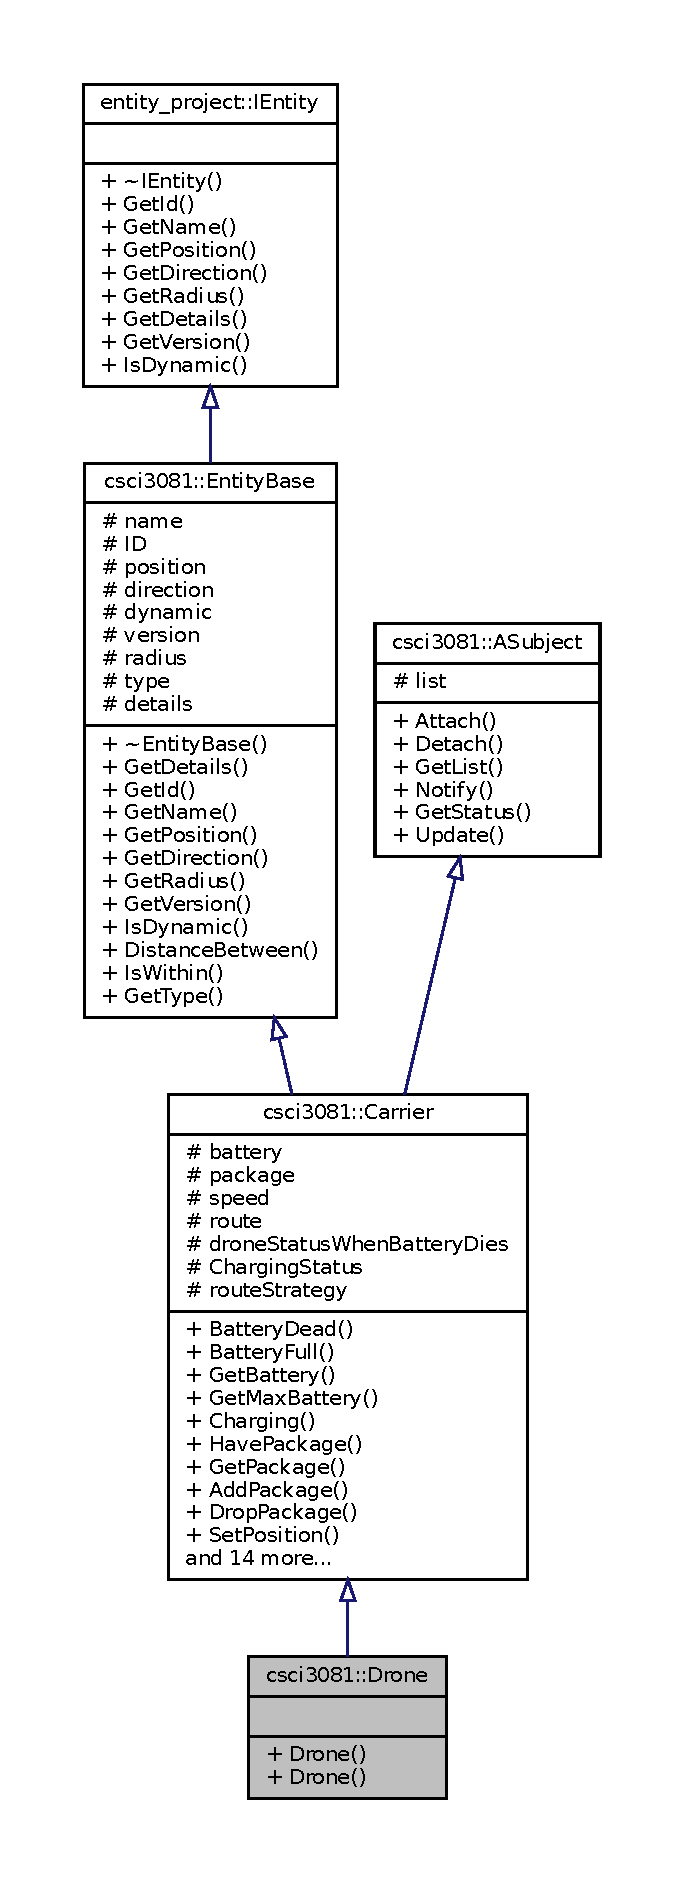
\includegraphics[height=550pt]{classcsci3081_1_1Drone__inherit__graph}
\end{center}
\end{figure}
\subsection*{Public Member Functions}
\begin{DoxyCompactItemize}
\item 
\hyperlink{classcsci3081_1_1Drone_ae6875af07d7f09ce59e2e2a62e5bd7d8}{Drone} (const picojson\+::object \&val)
\item 
\hyperlink{classcsci3081_1_1Drone_a2b97ed6144b5d97790e0950fa62d936f}{Drone} (\hyperlink{classcsci3081_1_1Drone}{Drone} \&)
\begin{DoxyCompactList}\small\item\em Copy Constructor. This creates a new instance of \hyperlink{classcsci3081_1_1Package}{Package} that has the same content as the \hyperlink{classcsci3081_1_1Package}{Package} argument. \end{DoxyCompactList}\end{DoxyCompactItemize}
\subsection*{Additional Inherited Members}


\subsection{Detailed Description}
A representation of a drone It stores the drone\textquotesingle{}s name, ID, version, position, direction, speed, and dynamic mode. 

\subsection{Constructor \& Destructor Documentation}
\mbox{\Hypertarget{classcsci3081_1_1Drone_ae6875af07d7f09ce59e2e2a62e5bd7d8}\label{classcsci3081_1_1Drone_ae6875af07d7f09ce59e2e2a62e5bd7d8}} 
\index{csci3081\+::\+Drone@{csci3081\+::\+Drone}!Drone@{Drone}}
\index{Drone@{Drone}!csci3081\+::\+Drone@{csci3081\+::\+Drone}}
\subsubsection{\texorpdfstring{Drone()}{Drone()}\hspace{0.1cm}{\footnotesize\ttfamily [1/2]}}
{\footnotesize\ttfamily csci3081\+::\+Drone\+::\+Drone (\begin{DoxyParamCaption}\item[{const picojson\+::object \&}]{val }\end{DoxyParamCaption})}

Constructor, creates a \hyperlink{classcsci3081_1_1Package}{Package} object param\mbox{[}in\mbox{]} val a picojson\+::object object that has the detail of the package including name, position, direction, radius, and speed \mbox{\Hypertarget{classcsci3081_1_1Drone_a2b97ed6144b5d97790e0950fa62d936f}\label{classcsci3081_1_1Drone_a2b97ed6144b5d97790e0950fa62d936f}} 
\index{csci3081\+::\+Drone@{csci3081\+::\+Drone}!Drone@{Drone}}
\index{Drone@{Drone}!csci3081\+::\+Drone@{csci3081\+::\+Drone}}
\subsubsection{\texorpdfstring{Drone()}{Drone()}\hspace{0.1cm}{\footnotesize\ttfamily [2/2]}}
{\footnotesize\ttfamily csci3081\+::\+Drone\+::\+Drone (\begin{DoxyParamCaption}\item[{\hyperlink{classcsci3081_1_1Drone}{Drone} \&}]{cpy }\end{DoxyParamCaption})}



Copy Constructor. This creates a new instance of \hyperlink{classcsci3081_1_1Package}{Package} that has the same content as the \hyperlink{classcsci3081_1_1Package}{Package} argument. 


\begin{DoxyParams}[1]{Parameters}
\mbox{\tt in}  & {\em cpy} & \hyperlink{classcsci3081_1_1Drone}{Drone} instance that wants to be copied \\
\hline
\end{DoxyParams}


The documentation for this class was generated from the following files\+:\begin{DoxyCompactItemize}
\item 
/home/user/repo/project/include/\hyperlink{drone_8h}{drone.\+h}\item 
/home/user/repo/project/src/drone.\+cc\end{DoxyCompactItemize}

\hypertarget{classcsci3081_1_1DroneFactory}{}\section{csci3081\+:\+:Drone\+Factory Class Reference}
\label{classcsci3081_1_1DroneFactory}\index{csci3081\+::\+Drone\+Factory@{csci3081\+::\+Drone\+Factory}}


This is the \hyperlink{classcsci3081_1_1DroneFactory}{Drone\+Factory}, responsible for making \hyperlink{classcsci3081_1_1Drone}{Drone} object.  




{\ttfamily \#include $<$drone\+\_\+factory.\+h$>$}



Inheritance diagram for csci3081\+:\+:Drone\+Factory\+:
\nopagebreak
\begin{figure}[H]
\begin{center}
\leavevmode
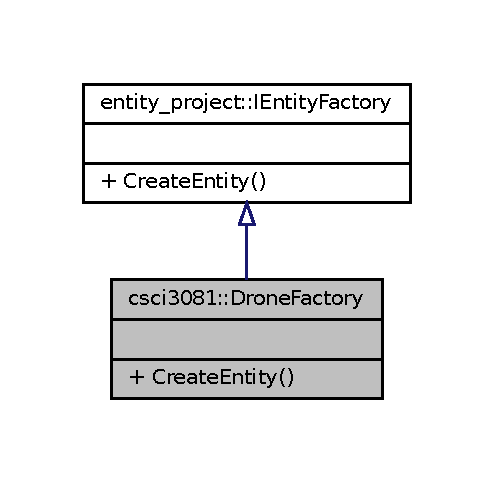
\includegraphics[width=237pt]{classcsci3081_1_1DroneFactory__inherit__graph}
\end{center}
\end{figure}
\subsection*{Public Member Functions}
\begin{DoxyCompactItemize}
\item 
\hyperlink{classentity__project_1_1IEntity}{I\+Entity} $\ast$ \hyperlink{classcsci3081_1_1DroneFactory_a84b3bc534c666c4485383bce502056b8}{Create\+Entity} (const picojson\+::object \&val)
\begin{DoxyCompactList}\small\item\em This is an inheritance function from I\+Entity\+Factory to create an approxiate Entity object based on the argument pass in Given the picojson\+::object val, this should create an entity. Based on the type of entity, there may be different fields. You can see the vals that will be passed in the project/web/scenes directory. Some of the fields are for our backend system and you don\textquotesingle{}t need to worry about them. (for instance, mesh, rotation, offset, etc.) \end{DoxyCompactList}\end{DoxyCompactItemize}


\subsection{Detailed Description}
This is the \hyperlink{classcsci3081_1_1DroneFactory}{Drone\+Factory}, responsible for making \hyperlink{classcsci3081_1_1Drone}{Drone} object. 

\subsection{Member Function Documentation}
\mbox{\Hypertarget{classcsci3081_1_1DroneFactory_a84b3bc534c666c4485383bce502056b8}\label{classcsci3081_1_1DroneFactory_a84b3bc534c666c4485383bce502056b8}} 
\index{csci3081\+::\+Drone\+Factory@{csci3081\+::\+Drone\+Factory}!Create\+Entity@{Create\+Entity}}
\index{Create\+Entity@{Create\+Entity}!csci3081\+::\+Drone\+Factory@{csci3081\+::\+Drone\+Factory}}
\subsubsection{\texorpdfstring{Create\+Entity()}{CreateEntity()}}
{\footnotesize\ttfamily \hyperlink{classentity__project_1_1IEntity}{I\+Entity} $\ast$ csci3081\+::\+Drone\+Factory\+::\+Create\+Entity (\begin{DoxyParamCaption}\item[{const picojson\+::object \&}]{val }\end{DoxyParamCaption})\hspace{0.3cm}{\ttfamily [virtual]}}



This is an inheritance function from I\+Entity\+Factory to create an approxiate Entity object based on the argument pass in Given the picojson\+::object val, this should create an entity. Based on the type of entity, there may be different fields. You can see the vals that will be passed in the project/web/scenes directory. Some of the fields are for our backend system and you don\textquotesingle{}t need to worry about them. (for instance, mesh, rotation, offset, etc.) 

Some fields in val that you will need to create the entity correctly\+:

type\+: string (could be \char`\"{}drone/customer/package\char`\"{})

name\+: string

position\+: array (contains \mbox{[}x\+\_\+position, y\+\_\+position, z\+\_\+position\mbox{]})

direction\+: array (contains \mbox{[}x, y, z\mbox{]})

speed\+: float

battery\+\_\+capacity\+: float 
\begin{DoxyParams}[1]{Parameters}
\mbox{\tt in}  & {\em val} & the picojson\+::object that constains all of the necessary information above in a json format \\
\hline
\end{DoxyParams}
\begin{DoxyReturn}{Returns}
I\+Entity pointer if the object has type \char`\"{}drone\char`\"{}; N\+U\+LL otherwise 
\end{DoxyReturn}


Implements \hyperlink{classentity__project_1_1IEntityFactory_ac4e8eaf4294958fef0b98bd3684704bb}{entity\+\_\+project\+::\+I\+Entity\+Factory}.



The documentation for this class was generated from the following files\+:\begin{DoxyCompactItemize}
\item 
/home/user/repo/project/include/\hyperlink{drone__factory_8h}{drone\+\_\+factory.\+h}\item 
/home/user/repo/project/src/drone\+\_\+factory.\+cc\end{DoxyCompactItemize}

\hypertarget{classcsci3081_1_1EntityBase}{}\section{csci3081\+:\+:Entity\+Base Class Reference}
\label{classcsci3081_1_1EntityBase}\index{csci3081\+::\+Entity\+Base@{csci3081\+::\+Entity\+Base}}


The base class for creating entities.  




{\ttfamily \#include $<$entity\+\_\+base.\+h$>$}



Inheritance diagram for csci3081\+:\+:Entity\+Base\+:
\nopagebreak
\begin{figure}[H]
\begin{center}
\leavevmode
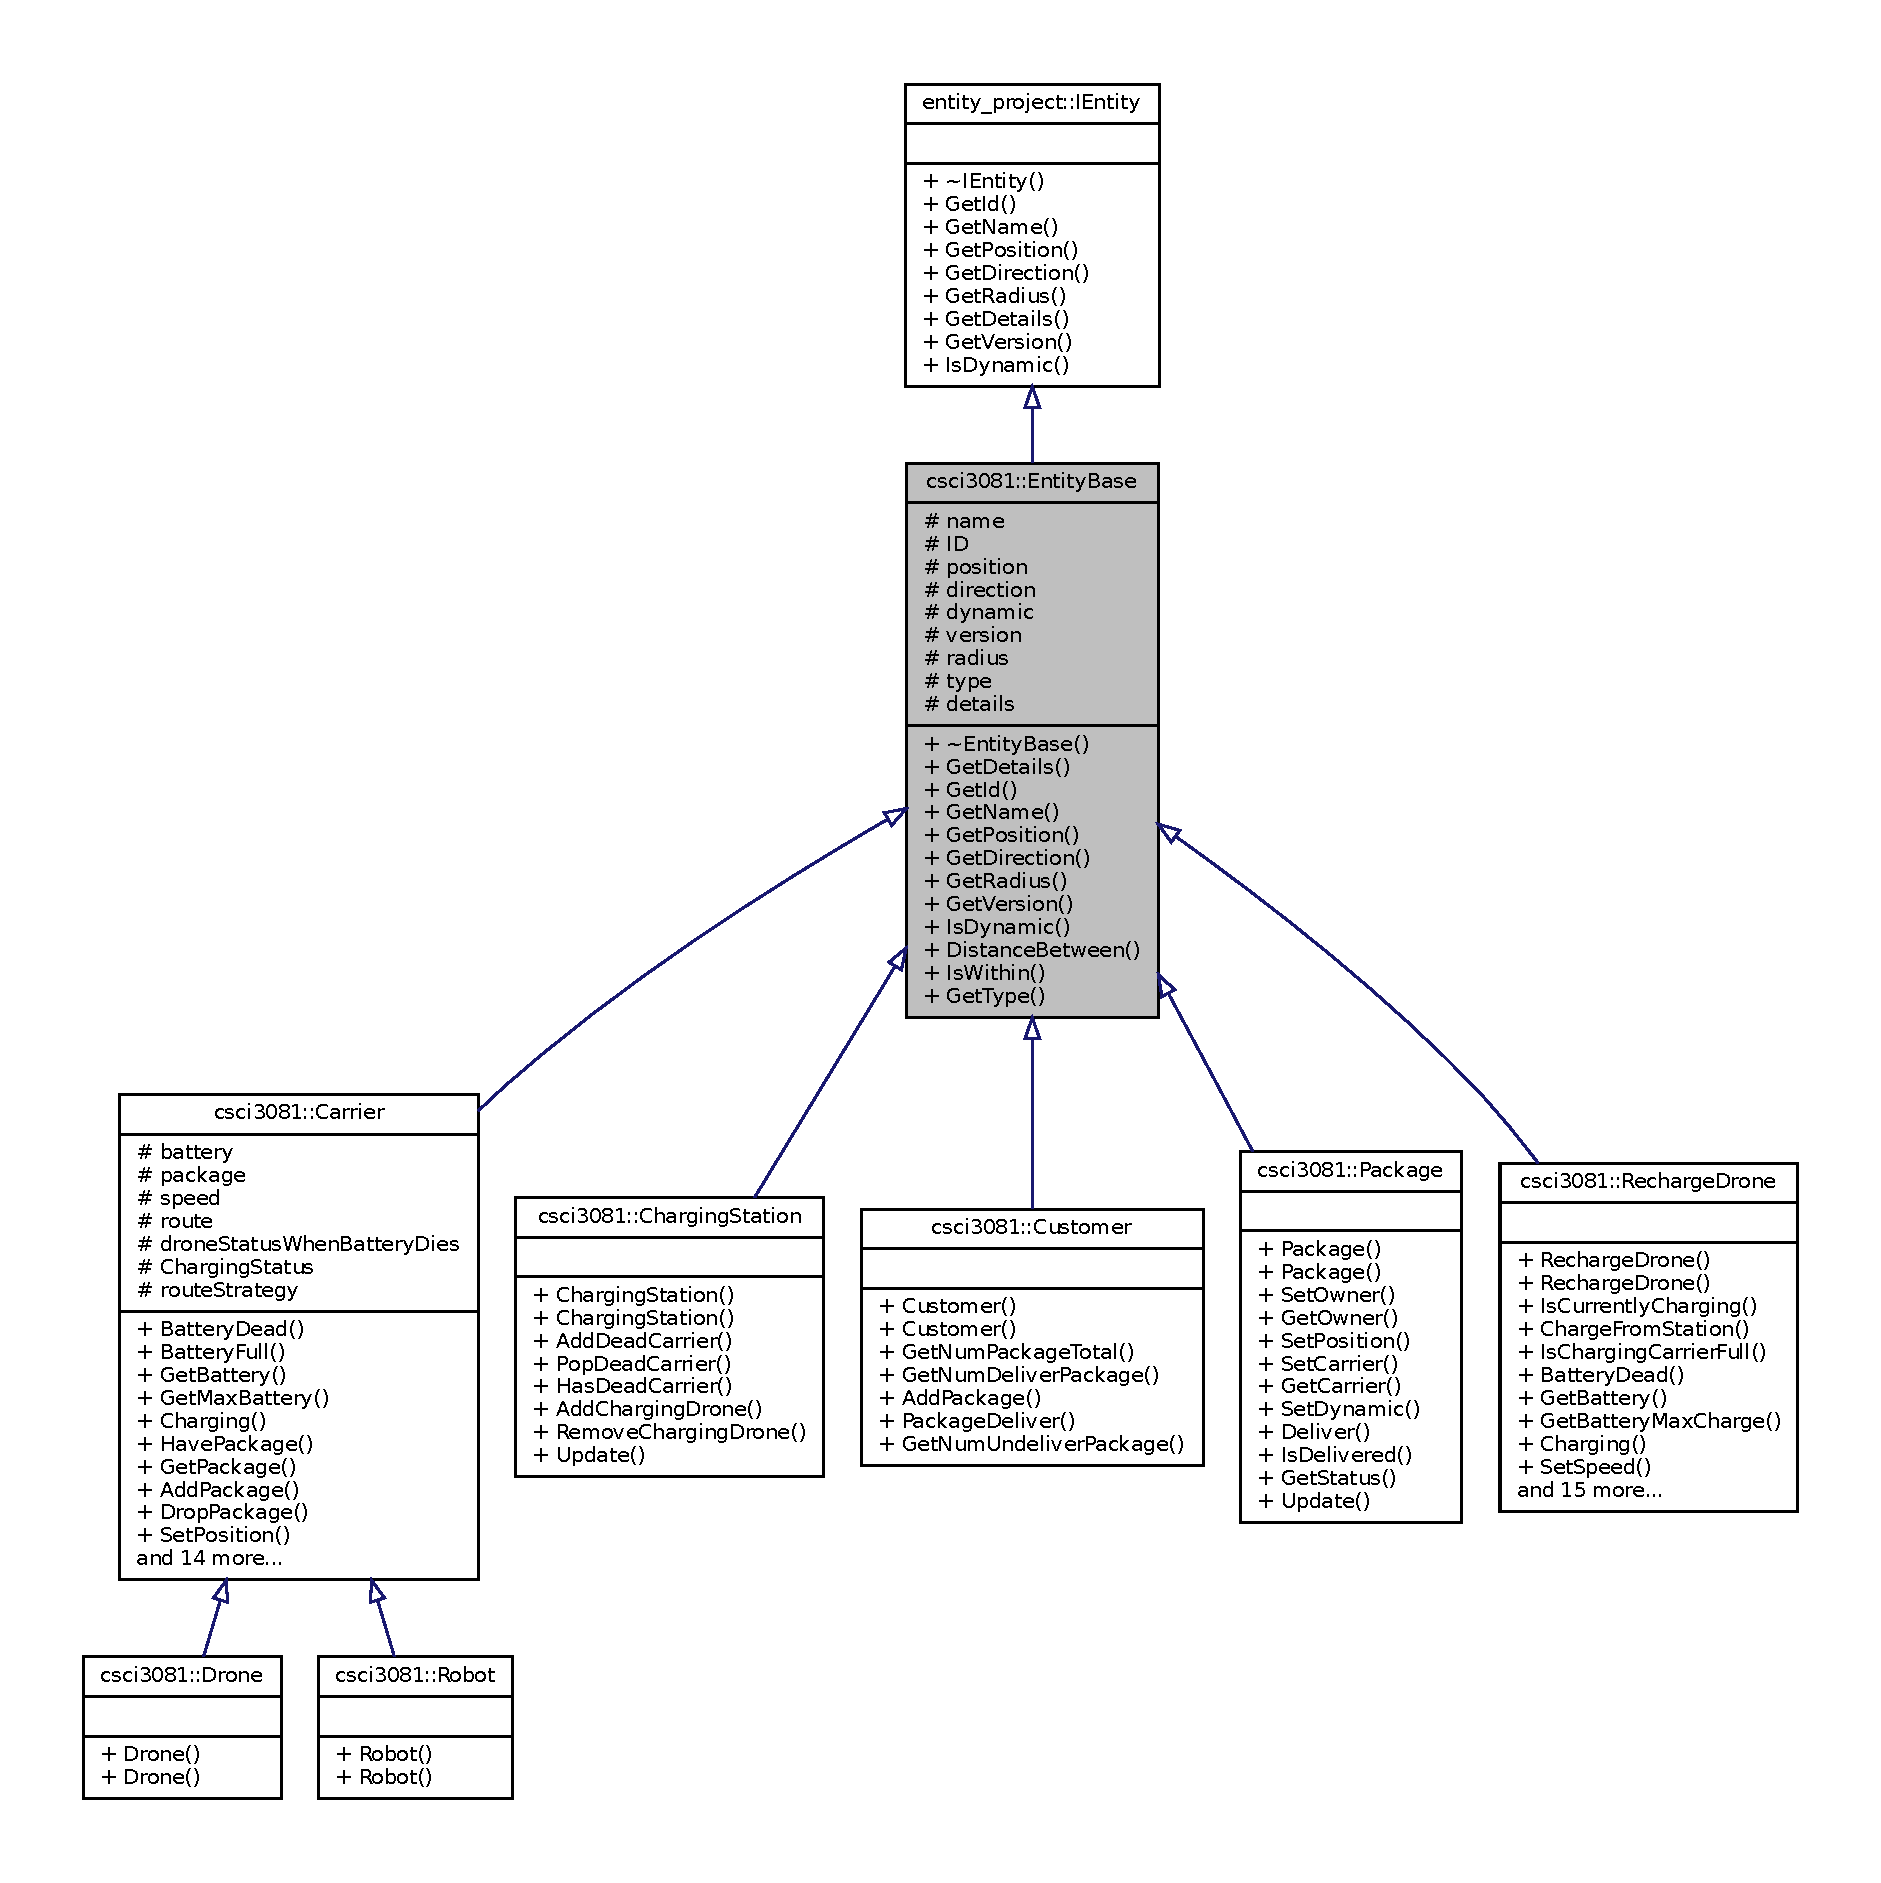
\includegraphics[width=350pt]{classcsci3081_1_1EntityBase__inherit__graph}
\end{center}
\end{figure}
\subsection*{Public Member Functions}
\begin{DoxyCompactItemize}
\item 
const picojson\+::object \& \hyperlink{classcsci3081_1_1EntityBase_aed18a7db12bfc8d6908ac6c28078110c}{Get\+Details} ()
\item 
int \hyperlink{classcsci3081_1_1EntityBase_a2802163d8d20092d985e763ad91d26da}{Get\+Id} () const
\item 
const std\+::string \& \hyperlink{classcsci3081_1_1EntityBase_ac18421e6e96eb3939e136a579c9ac6dd}{Get\+Name} ()
\item 
const std\+::vector$<$ float $>$ \& \hyperlink{classcsci3081_1_1EntityBase_a05830db8b41c0a9c05eec08f95f683ad}{Get\+Position} () const
\item 
const std\+::vector$<$ float $>$ \& \hyperlink{classcsci3081_1_1EntityBase_aeffff43e1d9b696b0ea3de83f7bee37d}{Get\+Direction} () const
\item 
float \hyperlink{classcsci3081_1_1EntityBase_abf61eb1cc8b94a7756f0ebc6a0c8a8f3}{Get\+Radius} () const
\item 
int \hyperlink{classcsci3081_1_1EntityBase_af5c87e8daf9161dc8c959c355b076bea}{Get\+Version} () const
\item 
bool \hyperlink{classcsci3081_1_1EntityBase_aa2a894f7821745acd91fbfb2e2e92082}{Is\+Dynamic} () const
\item 
float \hyperlink{classcsci3081_1_1EntityBase_a41270ec9049d9d0a379987ab95796bd9}{Distance\+Between} (\hyperlink{classentity__project_1_1IEntity}{I\+Entity} $\ast$another)
\item 
bool \hyperlink{classcsci3081_1_1EntityBase_a7ed05da61dab982c517c3481941a4be8}{Is\+Within} (\hyperlink{classentity__project_1_1IEntity}{I\+Entity} $\ast$another)
\item 
std\+::string \hyperlink{classcsci3081_1_1EntityBase_ac2efc31e2a346b29897f711c44b71ecb}{Get\+Type} ()
\end{DoxyCompactItemize}
\subsection*{Protected Attributes}
\begin{DoxyCompactItemize}
\item 
\mbox{\Hypertarget{classcsci3081_1_1EntityBase_ac38853fd49f990fbf4a5253f6a629830}\label{classcsci3081_1_1EntityBase_ac38853fd49f990fbf4a5253f6a629830}} 
std\+::string {\bfseries name}
\item 
\mbox{\Hypertarget{classcsci3081_1_1EntityBase_aac37ea7e640a8a710b3b5ac1f8c721ab}\label{classcsci3081_1_1EntityBase_aac37ea7e640a8a710b3b5ac1f8c721ab}} 
int {\bfseries ID}
\item 
\mbox{\Hypertarget{classcsci3081_1_1EntityBase_aab57c1d92706e8a78b85a159df6955e9}\label{classcsci3081_1_1EntityBase_aab57c1d92706e8a78b85a159df6955e9}} 
std\+::vector$<$ float $>$ {\bfseries position}
\item 
\mbox{\Hypertarget{classcsci3081_1_1EntityBase_a76a2b78baa728973a7e3e4608224840e}\label{classcsci3081_1_1EntityBase_a76a2b78baa728973a7e3e4608224840e}} 
std\+::vector$<$ float $>$ {\bfseries direction}
\item 
\mbox{\Hypertarget{classcsci3081_1_1EntityBase_ad4623718110440313bf7ee316838a352}\label{classcsci3081_1_1EntityBase_ad4623718110440313bf7ee316838a352}} 
bool {\bfseries dynamic}
\item 
\mbox{\Hypertarget{classcsci3081_1_1EntityBase_ae4224835873699684a7b7a1ea39fdf77}\label{classcsci3081_1_1EntityBase_ae4224835873699684a7b7a1ea39fdf77}} 
int {\bfseries version}
\item 
\mbox{\Hypertarget{classcsci3081_1_1EntityBase_ae2c7b177b5038a5a369046ae577ef19e}\label{classcsci3081_1_1EntityBase_ae2c7b177b5038a5a369046ae577ef19e}} 
float {\bfseries radius}
\item 
\mbox{\Hypertarget{classcsci3081_1_1EntityBase_aed45722b1b5a3b0f191084139d47c051}\label{classcsci3081_1_1EntityBase_aed45722b1b5a3b0f191084139d47c051}} 
std\+::string {\bfseries type}
\item 
\mbox{\Hypertarget{classcsci3081_1_1EntityBase_a75477f89357da1cc9ac999ec6bd6db5b}\label{classcsci3081_1_1EntityBase_a75477f89357da1cc9ac999ec6bd6db5b}} 
picojson\+::object {\bfseries details}
\end{DoxyCompactItemize}


\subsection{Detailed Description}
The base class for creating entities. 

This class can be used as the base for all entities in the delivery system. The overall design is up to you (the student), but all entities must implement the I\+Entity interface.

See the documentation for I\+Entity for more information 

\subsection{Member Function Documentation}
\mbox{\Hypertarget{classcsci3081_1_1EntityBase_a41270ec9049d9d0a379987ab95796bd9}\label{classcsci3081_1_1EntityBase_a41270ec9049d9d0a379987ab95796bd9}} 
\index{csci3081\+::\+Entity\+Base@{csci3081\+::\+Entity\+Base}!Distance\+Between@{Distance\+Between}}
\index{Distance\+Between@{Distance\+Between}!csci3081\+::\+Entity\+Base@{csci3081\+::\+Entity\+Base}}
\subsubsection{\texorpdfstring{Distance\+Between()}{DistanceBetween()}}
{\footnotesize\ttfamily float csci3081\+::\+Entity\+Base\+::\+Distance\+Between (\begin{DoxyParamCaption}\item[{\hyperlink{classentity__project_1_1IEntity}{I\+Entity} $\ast$}]{another }\end{DoxyParamCaption})}

Return the distance between the I\+Entity objects \mbox{\Hypertarget{classcsci3081_1_1EntityBase_aed18a7db12bfc8d6908ac6c28078110c}\label{classcsci3081_1_1EntityBase_aed18a7db12bfc8d6908ac6c28078110c}} 
\index{csci3081\+::\+Entity\+Base@{csci3081\+::\+Entity\+Base}!Get\+Details@{Get\+Details}}
\index{Get\+Details@{Get\+Details}!csci3081\+::\+Entity\+Base@{csci3081\+::\+Entity\+Base}}
\subsubsection{\texorpdfstring{Get\+Details()}{GetDetails()}}
{\footnotesize\ttfamily const picojson\+::object \& csci3081\+::\+Entity\+Base\+::\+Get\+Details (\begin{DoxyParamCaption}{ }\end{DoxyParamCaption})\hspace{0.3cm}{\ttfamily [virtual]}}

Returns the entity\textquotesingle{}s details. The returned picojson\+::object should be a copy of the json that was passed in when the entity was created. Details are also used to send additional information to other subsystems (e.\+g. mesh, scale, rotation, etc...). 

Implements \hyperlink{classentity__project_1_1IEntity_a73c5b6deac9e2659160d2952ae7572c4}{entity\+\_\+project\+::\+I\+Entity}.

\mbox{\Hypertarget{classcsci3081_1_1EntityBase_aeffff43e1d9b696b0ea3de83f7bee37d}\label{classcsci3081_1_1EntityBase_aeffff43e1d9b696b0ea3de83f7bee37d}} 
\index{csci3081\+::\+Entity\+Base@{csci3081\+::\+Entity\+Base}!Get\+Direction@{Get\+Direction}}
\index{Get\+Direction@{Get\+Direction}!csci3081\+::\+Entity\+Base@{csci3081\+::\+Entity\+Base}}
\subsubsection{\texorpdfstring{Get\+Direction()}{GetDirection()}}
{\footnotesize\ttfamily const std\+::vector$<$ float $>$ \& csci3081\+::\+Entity\+Base\+::\+Get\+Direction (\begin{DoxyParamCaption}{ }\end{DoxyParamCaption}) const\hspace{0.3cm}{\ttfamily [virtual]}}

Return the direction of the drone param \mbox{[}out\mbox{]}\+: direction of the drone as vector of float 

Implements \hyperlink{classentity__project_1_1IEntity_a385dad034b5a86666df9fc979a3d1d1b}{entity\+\_\+project\+::\+I\+Entity}.

\mbox{\Hypertarget{classcsci3081_1_1EntityBase_a2802163d8d20092d985e763ad91d26da}\label{classcsci3081_1_1EntityBase_a2802163d8d20092d985e763ad91d26da}} 
\index{csci3081\+::\+Entity\+Base@{csci3081\+::\+Entity\+Base}!Get\+Id@{Get\+Id}}
\index{Get\+Id@{Get\+Id}!csci3081\+::\+Entity\+Base@{csci3081\+::\+Entity\+Base}}
\subsubsection{\texorpdfstring{Get\+Id()}{GetId()}}
{\footnotesize\ttfamily int csci3081\+::\+Entity\+Base\+::\+Get\+Id (\begin{DoxyParamCaption}{ }\end{DoxyParamCaption}) const\hspace{0.3cm}{\ttfamily [virtual]}}

Return the unique ID of the drone param \mbox{[}out\mbox{]}\+: ID of the drone 

Implements \hyperlink{classentity__project_1_1IEntity_a87f9d99f58cdc28b654ae9a6d82fbff6}{entity\+\_\+project\+::\+I\+Entity}.

\mbox{\Hypertarget{classcsci3081_1_1EntityBase_ac18421e6e96eb3939e136a579c9ac6dd}\label{classcsci3081_1_1EntityBase_ac18421e6e96eb3939e136a579c9ac6dd}} 
\index{csci3081\+::\+Entity\+Base@{csci3081\+::\+Entity\+Base}!Get\+Name@{Get\+Name}}
\index{Get\+Name@{Get\+Name}!csci3081\+::\+Entity\+Base@{csci3081\+::\+Entity\+Base}}
\subsubsection{\texorpdfstring{Get\+Name()}{GetName()}}
{\footnotesize\ttfamily const std\+::string \& csci3081\+::\+Entity\+Base\+::\+Get\+Name (\begin{DoxyParamCaption}{ }\end{DoxyParamCaption})\hspace{0.3cm}{\ttfamily [virtual]}}

Return the name of the drone param \mbox{[}out\mbox{]}\+: name of the drone 

Implements \hyperlink{classentity__project_1_1IEntity_a60fe17f543af26a48181a0c290a822ab}{entity\+\_\+project\+::\+I\+Entity}.

\mbox{\Hypertarget{classcsci3081_1_1EntityBase_a05830db8b41c0a9c05eec08f95f683ad}\label{classcsci3081_1_1EntityBase_a05830db8b41c0a9c05eec08f95f683ad}} 
\index{csci3081\+::\+Entity\+Base@{csci3081\+::\+Entity\+Base}!Get\+Position@{Get\+Position}}
\index{Get\+Position@{Get\+Position}!csci3081\+::\+Entity\+Base@{csci3081\+::\+Entity\+Base}}
\subsubsection{\texorpdfstring{Get\+Position()}{GetPosition()}}
{\footnotesize\ttfamily const std\+::vector$<$ float $>$ \& csci3081\+::\+Entity\+Base\+::\+Get\+Position (\begin{DoxyParamCaption}{ }\end{DoxyParamCaption}) const\hspace{0.3cm}{\ttfamily [virtual]}}

Return the position of the drone param \mbox{[}out\mbox{]}\+: position of the drone as vector of float 

Implements \hyperlink{classentity__project_1_1IEntity_a1369c59d258645a12a06239ece1134cf}{entity\+\_\+project\+::\+I\+Entity}.

\mbox{\Hypertarget{classcsci3081_1_1EntityBase_abf61eb1cc8b94a7756f0ebc6a0c8a8f3}\label{classcsci3081_1_1EntityBase_abf61eb1cc8b94a7756f0ebc6a0c8a8f3}} 
\index{csci3081\+::\+Entity\+Base@{csci3081\+::\+Entity\+Base}!Get\+Radius@{Get\+Radius}}
\index{Get\+Radius@{Get\+Radius}!csci3081\+::\+Entity\+Base@{csci3081\+::\+Entity\+Base}}
\subsubsection{\texorpdfstring{Get\+Radius()}{GetRadius()}}
{\footnotesize\ttfamily float csci3081\+::\+Entity\+Base\+::\+Get\+Radius (\begin{DoxyParamCaption}{ }\end{DoxyParamCaption}) const\hspace{0.3cm}{\ttfamily [virtual]}}

Return the radius of the drone param \mbox{[}out\mbox{]}\+: radius of the drone as vector of float 

Implements \hyperlink{classentity__project_1_1IEntity_af2c2f81a5d201c4c1968f055808ba59c}{entity\+\_\+project\+::\+I\+Entity}.

\mbox{\Hypertarget{classcsci3081_1_1EntityBase_ac2efc31e2a346b29897f711c44b71ecb}\label{classcsci3081_1_1EntityBase_ac2efc31e2a346b29897f711c44b71ecb}} 
\index{csci3081\+::\+Entity\+Base@{csci3081\+::\+Entity\+Base}!Get\+Type@{Get\+Type}}
\index{Get\+Type@{Get\+Type}!csci3081\+::\+Entity\+Base@{csci3081\+::\+Entity\+Base}}
\subsubsection{\texorpdfstring{Get\+Type()}{GetType()}}
{\footnotesize\ttfamily std\+::string csci3081\+::\+Entity\+Base\+::\+Get\+Type (\begin{DoxyParamCaption}{ }\end{DoxyParamCaption})}

Return std\+::string type of the Entity object, such as \char`\"{}carrier\char`\"{} and \char`\"{}customer\char`\"{} \mbox{\Hypertarget{classcsci3081_1_1EntityBase_af5c87e8daf9161dc8c959c355b076bea}\label{classcsci3081_1_1EntityBase_af5c87e8daf9161dc8c959c355b076bea}} 
\index{csci3081\+::\+Entity\+Base@{csci3081\+::\+Entity\+Base}!Get\+Version@{Get\+Version}}
\index{Get\+Version@{Get\+Version}!csci3081\+::\+Entity\+Base@{csci3081\+::\+Entity\+Base}}
\subsubsection{\texorpdfstring{Get\+Version()}{GetVersion()}}
{\footnotesize\ttfamily int csci3081\+::\+Entity\+Base\+::\+Get\+Version (\begin{DoxyParamCaption}{ }\end{DoxyParamCaption}) const\hspace{0.3cm}{\ttfamily [virtual]}}

Return the version of the drone param \mbox{[}out\mbox{]}\+: version of the drone as vector of float 

Implements \hyperlink{classentity__project_1_1IEntity_a254b8c22f103ebf23261cb79bc121118}{entity\+\_\+project\+::\+I\+Entity}.

\mbox{\Hypertarget{classcsci3081_1_1EntityBase_aa2a894f7821745acd91fbfb2e2e92082}\label{classcsci3081_1_1EntityBase_aa2a894f7821745acd91fbfb2e2e92082}} 
\index{csci3081\+::\+Entity\+Base@{csci3081\+::\+Entity\+Base}!Is\+Dynamic@{Is\+Dynamic}}
\index{Is\+Dynamic@{Is\+Dynamic}!csci3081\+::\+Entity\+Base@{csci3081\+::\+Entity\+Base}}
\subsubsection{\texorpdfstring{Is\+Dynamic()}{IsDynamic()}}
{\footnotesize\ttfamily bool csci3081\+::\+Entity\+Base\+::\+Is\+Dynamic (\begin{DoxyParamCaption}{ }\end{DoxyParamCaption}) const\hspace{0.3cm}{\ttfamily [virtual]}}

Return the dynamic of the drone param \mbox{[}out\mbox{]}\+: dynamic of the drone as vector of float 

Implements \hyperlink{classentity__project_1_1IEntity_a58d710abd04e533123d033a7ba80f017}{entity\+\_\+project\+::\+I\+Entity}.

\mbox{\Hypertarget{classcsci3081_1_1EntityBase_a7ed05da61dab982c517c3481941a4be8}\label{classcsci3081_1_1EntityBase_a7ed05da61dab982c517c3481941a4be8}} 
\index{csci3081\+::\+Entity\+Base@{csci3081\+::\+Entity\+Base}!Is\+Within@{Is\+Within}}
\index{Is\+Within@{Is\+Within}!csci3081\+::\+Entity\+Base@{csci3081\+::\+Entity\+Base}}
\subsubsection{\texorpdfstring{Is\+Within()}{IsWithin()}}
{\footnotesize\ttfamily bool csci3081\+::\+Entity\+Base\+::\+Is\+Within (\begin{DoxyParamCaption}\item[{\hyperlink{classentity__project_1_1IEntity}{I\+Entity} $\ast$}]{another }\end{DoxyParamCaption})}

Return true if the object is within radius of the I\+Entity object passed in the argument; Return false otherwise 

The documentation for this class was generated from the following files\+:\begin{DoxyCompactItemize}
\item 
/home/user/repo/project/include/\hyperlink{entity__base_8h}{entity\+\_\+base.\+h}\item 
/home/user/repo/project/src/entity\+\_\+base.\+cc\end{DoxyCompactItemize}

\hypertarget{classentity__project_1_1EntityConsoleLogger}{}\section{entity\+\_\+project\+:\+:Entity\+Console\+Logger Class Reference}
\label{classentity__project_1_1EntityConsoleLogger}\index{entity\+\_\+project\+::\+Entity\+Console\+Logger@{entity\+\_\+project\+::\+Entity\+Console\+Logger}}


The Entity Console Logger outputs entity events to the command line.  




{\ttfamily \#include $<$entity\+\_\+console\+\_\+logger.\+h$>$}



Inheritance diagram for entity\+\_\+project\+:\+:Entity\+Console\+Logger\+:
\nopagebreak
\begin{figure}[H]
\begin{center}
\leavevmode
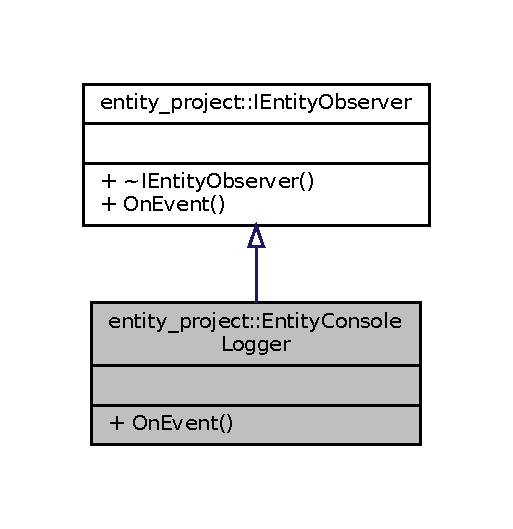
\includegraphics[width=246pt]{classentity__project_1_1EntityConsoleLogger__inherit__graph}
\end{center}
\end{figure}
\subsection*{Public Member Functions}
\begin{DoxyCompactItemize}
\item 
\mbox{\Hypertarget{classentity__project_1_1EntityConsoleLogger_a5079a172a767e164df8016ce06a3ce4e}\label{classentity__project_1_1EntityConsoleLogger_a5079a172a767e164df8016ce06a3ce4e}} 
virtual void \hyperlink{classentity__project_1_1EntityConsoleLogger_a5079a172a767e164df8016ce06a3ce4e}{On\+Event} (const picojson\+::value \&event, const \hyperlink{classentity__project_1_1IEntity}{I\+Entity} \&entity)
\begin{DoxyCompactList}\small\item\em Callback when an event happens. \end{DoxyCompactList}\end{DoxyCompactItemize}


\subsection{Detailed Description}
The Entity Console Logger outputs entity events to the command line. 

The documentation for this class was generated from the following file\+:\begin{DoxyCompactItemize}
\item 
/home/user/repo/.\+dependencies/include/\+Entity\+Project/entity\+\_\+console\+\_\+logger.\+h\end{DoxyCompactItemize}

\hypertarget{classcsci3081_1_1GenerateId}{}\section{csci3081\+:\+:Generate\+Id Class Reference}
\label{classcsci3081_1_1GenerateId}\index{csci3081\+::\+Generate\+Id@{csci3081\+::\+Generate\+Id}}


\hyperlink{classcsci3081_1_1GenerateId}{Generate\+Id} class generates a static unique identifier to the customer, drone, robot, package, and battery objects. Each time \hyperlink{classcsci3081_1_1GenerateId_a26a75b8750133b7624199a29c5620dd5}{Generate\+New\+Id()} is called, the {\ttfamily id} variable gets incremented.  




{\ttfamily \#include $<$generate\+\_\+id.\+h$>$}

\subsection*{Public Member Functions}
\begin{DoxyCompactItemize}
\item 
int \hyperlink{classcsci3081_1_1GenerateId_afb9af0fc5150212ef877a786fa597c9b}{Reset\+Id} ()
\end{DoxyCompactItemize}
\subsection*{Static Public Member Functions}
\begin{DoxyCompactItemize}
\item 
static int \hyperlink{classcsci3081_1_1GenerateId_a26a75b8750133b7624199a29c5620dd5}{Generate\+New\+Id} ()
\end{DoxyCompactItemize}


\subsection{Detailed Description}
\hyperlink{classcsci3081_1_1GenerateId}{Generate\+Id} class generates a static unique identifier to the customer, drone, robot, package, and battery objects. Each time \hyperlink{classcsci3081_1_1GenerateId_a26a75b8750133b7624199a29c5620dd5}{Generate\+New\+Id()} is called, the {\ttfamily id} variable gets incremented. 

\subsection{Member Function Documentation}
\mbox{\Hypertarget{classcsci3081_1_1GenerateId_a26a75b8750133b7624199a29c5620dd5}\label{classcsci3081_1_1GenerateId_a26a75b8750133b7624199a29c5620dd5}} 
\index{csci3081\+::\+Generate\+Id@{csci3081\+::\+Generate\+Id}!Generate\+New\+Id@{Generate\+New\+Id}}
\index{Generate\+New\+Id@{Generate\+New\+Id}!csci3081\+::\+Generate\+Id@{csci3081\+::\+Generate\+Id}}
\subsubsection{\texorpdfstring{Generate\+New\+Id()}{GenerateNewId()}}
{\footnotesize\ttfamily int csci3081\+::\+Generate\+Id\+::\+Generate\+New\+Id (\begin{DoxyParamCaption}{ }\end{DoxyParamCaption})\hspace{0.3cm}{\ttfamily [static]}}

This function statically increments the ID counter to create a unique identifier. \mbox{\Hypertarget{classcsci3081_1_1GenerateId_afb9af0fc5150212ef877a786fa597c9b}\label{classcsci3081_1_1GenerateId_afb9af0fc5150212ef877a786fa597c9b}} 
\index{csci3081\+::\+Generate\+Id@{csci3081\+::\+Generate\+Id}!Reset\+Id@{Reset\+Id}}
\index{Reset\+Id@{Reset\+Id}!csci3081\+::\+Generate\+Id@{csci3081\+::\+Generate\+Id}}
\subsubsection{\texorpdfstring{Reset\+Id()}{ResetId()}}
{\footnotesize\ttfamily int csci3081\+::\+Generate\+Id\+::\+Reset\+Id (\begin{DoxyParamCaption}{ }\end{DoxyParamCaption})}

Warning\+: this function S\+H\+O\+U\+LD O\+N\+LY BE C\+A\+L\+L\+ED during Google Test cases. This function resets the ID counter back to 0. \begin{DoxyReturn}{Returns}
Current reset ID. 
\end{DoxyReturn}


The documentation for this class was generated from the following files\+:\begin{DoxyCompactItemize}
\item 
/home/user/repo/project/include/generate\+\_\+id.\+h\item 
/home/user/repo/project/src/generate\+\_\+id.\+cc\end{DoxyCompactItemize}

\hypertarget{classcsci3081_1_1IDeliverySystem}{}\section{csci3081\+:\+:I\+Delivery\+System Class Reference}
\label{classcsci3081_1_1IDeliverySystem}\index{csci3081\+::\+I\+Delivery\+System@{csci3081\+::\+I\+Delivery\+System}}


The abstract facade of a drone delivery subsystem.  




{\ttfamily \#include $<$delivery\+\_\+system.\+h$>$}



Inheritance diagram for csci3081\+:\+:I\+Delivery\+System\+:
\nopagebreak
\begin{figure}[H]
\begin{center}
\leavevmode
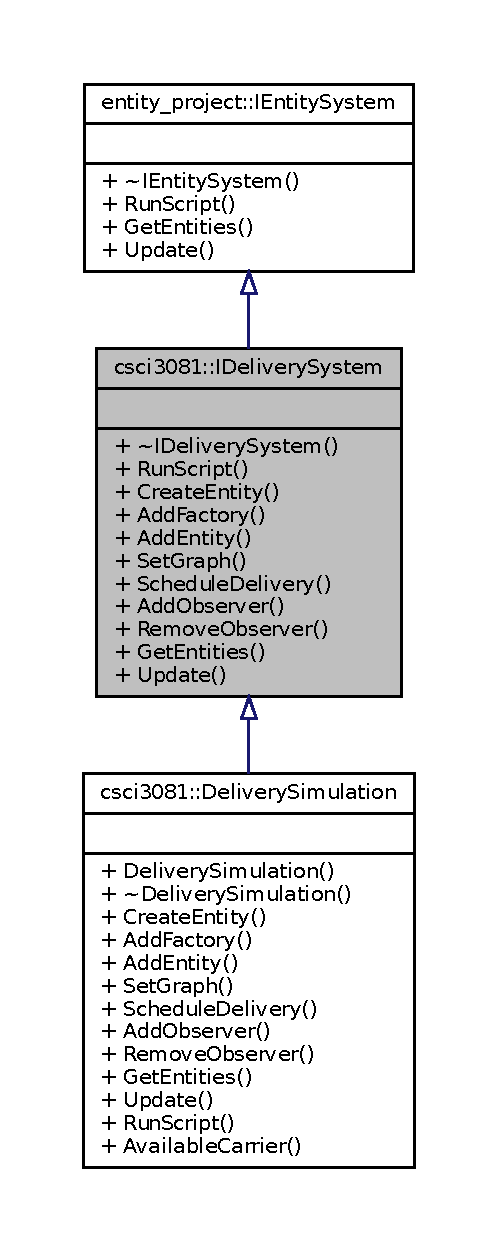
\includegraphics[height=550pt]{classcsci3081_1_1IDeliverySystem__inherit__graph}
\end{center}
\end{figure}
\subsection*{Public Member Functions}
\begin{DoxyCompactItemize}
\item 
\mbox{\Hypertarget{classcsci3081_1_1IDeliverySystem_a756634386c8a889ca93ba0e2fc960155}\label{classcsci3081_1_1IDeliverySystem_a756634386c8a889ca93ba0e2fc960155}} 
virtual \hyperlink{classcsci3081_1_1IDeliverySystem_a756634386c8a889ca93ba0e2fc960155}{$\sim$\+I\+Delivery\+System} ()
\begin{DoxyCompactList}\small\item\em Destructor. \end{DoxyCompactList}\item 
virtual void \hyperlink{classcsci3081_1_1IDeliverySystem_ae152276130e859b052f1d89417be6fc2}{Run\+Script} (const picojson\+::array \&script, \hyperlink{classentity__project_1_1IEntitySystem}{I\+Entity\+System} $\ast$system) const =0
\begin{DoxyCompactList}\small\item\em Translates a set of J\+S\+ON commands into method calls for the drone delivery system. \end{DoxyCompactList}\item 
virtual \hyperlink{classentity__project_1_1IEntity}{I\+Entity} $\ast$ \hyperlink{classcsci3081_1_1IDeliverySystem_abc1959b16d1fcfdeea2a2d8af0733301}{Create\+Entity} (const picojson\+::object \&val)=0
\begin{DoxyCompactList}\small\item\em Creates an entity based on a J\+S\+ON object passed in. \end{DoxyCompactList}\item 
\mbox{\Hypertarget{classcsci3081_1_1IDeliverySystem_a4d6a5fa94ab597dbe88ae0046d698e76}\label{classcsci3081_1_1IDeliverySystem_a4d6a5fa94ab597dbe88ae0046d698e76}} 
virtual void \hyperlink{classcsci3081_1_1IDeliverySystem_a4d6a5fa94ab597dbe88ae0046d698e76}{Add\+Factory} (\hyperlink{classentity__project_1_1IEntityFactory}{I\+Entity\+Factory} $\ast$factory)=0
\begin{DoxyCompactList}\small\item\em Adds an entity factory to a composite factory for creating new entities. \end{DoxyCompactList}\item 
\mbox{\Hypertarget{classcsci3081_1_1IDeliverySystem_ae8fe57f0627f3429d4a8cea4d910e233}\label{classcsci3081_1_1IDeliverySystem_ae8fe57f0627f3429d4a8cea4d910e233}} 
virtual void \hyperlink{classcsci3081_1_1IDeliverySystem_ae8fe57f0627f3429d4a8cea4d910e233}{Add\+Entity} (\hyperlink{classentity__project_1_1IEntity}{I\+Entity} $\ast$entity)=0
\begin{DoxyCompactList}\small\item\em Adds an entity to an entity vector member. Once added, entities can be affected by the system. \end{DoxyCompactList}\item 
\mbox{\Hypertarget{classcsci3081_1_1IDeliverySystem_ac379454e54cc392ff7c24f565a3e8353}\label{classcsci3081_1_1IDeliverySystem_ac379454e54cc392ff7c24f565a3e8353}} 
virtual void \hyperlink{classcsci3081_1_1IDeliverySystem_ac379454e54cc392ff7c24f565a3e8353}{Set\+Graph} (const \hyperlink{classentity__project_1_1IGraph}{I\+Graph} $\ast$graph)=0
\begin{DoxyCompactList}\small\item\em Adds the graph used for dynamic routing in the delivery system. \end{DoxyCompactList}\item 
virtual void \hyperlink{classcsci3081_1_1IDeliverySystem_a25210b242623675309c16e8a2c3cfd0e}{Schedule\+Delivery} (\hyperlink{classentity__project_1_1IEntity}{I\+Entity} $\ast$package, \hyperlink{classentity__project_1_1IEntity}{I\+Entity} $\ast$dest)=0
\begin{DoxyCompactList}\small\item\em Schedule a drone delivery for a package to be delivered to a customer. \end{DoxyCompactList}\item 
\mbox{\Hypertarget{classcsci3081_1_1IDeliverySystem_a53161d8f9f94ee5f56e39f98b52ac3e2}\label{classcsci3081_1_1IDeliverySystem_a53161d8f9f94ee5f56e39f98b52ac3e2}} 
virtual void \hyperlink{classcsci3081_1_1IDeliverySystem_a53161d8f9f94ee5f56e39f98b52ac3e2}{Add\+Observer} (\hyperlink{classentity__project_1_1IEntityObserver}{I\+Entity\+Observer} $\ast$observer)=0
\begin{DoxyCompactList}\small\item\em Add an observer to a specific entity. \end{DoxyCompactList}\item 
\mbox{\Hypertarget{classcsci3081_1_1IDeliverySystem_a79d4336f9fd4bcb837a5be1713f84ab1}\label{classcsci3081_1_1IDeliverySystem_a79d4336f9fd4bcb837a5be1713f84ab1}} 
virtual void \hyperlink{classcsci3081_1_1IDeliverySystem_a79d4336f9fd4bcb837a5be1713f84ab1}{Remove\+Observer} (\hyperlink{classentity__project_1_1IEntityObserver}{I\+Entity\+Observer} $\ast$observer)=0
\begin{DoxyCompactList}\small\item\em Remove an observer from a specific entity. \end{DoxyCompactList}\item 
\mbox{\Hypertarget{classcsci3081_1_1IDeliverySystem_aca4e7e3e9a9a19ca87f788935b882277}\label{classcsci3081_1_1IDeliverySystem_aca4e7e3e9a9a19ca87f788935b882277}} 
virtual const std\+::vector$<$ \hyperlink{classentity__project_1_1IEntity}{I\+Entity} $\ast$ $>$ \& \hyperlink{classcsci3081_1_1IDeliverySystem_aca4e7e3e9a9a19ca87f788935b882277}{Get\+Entities} () const =0
\begin{DoxyCompactList}\small\item\em Returns all the entities that are added to the drone system. \end{DoxyCompactList}\item 
\mbox{\Hypertarget{classcsci3081_1_1IDeliverySystem_a3ef0dda19a6e1ad322bb6dd35ae3e3f1}\label{classcsci3081_1_1IDeliverySystem_a3ef0dda19a6e1ad322bb6dd35ae3e3f1}} 
virtual void \hyperlink{classcsci3081_1_1IDeliverySystem_a3ef0dda19a6e1ad322bb6dd35ae3e3f1}{Update} (float dt)=0
\begin{DoxyCompactList}\small\item\em Updates the drone system time by dt. \end{DoxyCompactList}\end{DoxyCompactItemize}


\subsection{Detailed Description}
The abstract facade of a drone delivery subsystem. 

U\+S\+A\+GE\+: this class is meant to be inherited by a delivery system class you create. Extend this class to manage the drone delivery subsystem of entities. 

\subsection{Member Function Documentation}
\mbox{\Hypertarget{classcsci3081_1_1IDeliverySystem_abc1959b16d1fcfdeea2a2d8af0733301}\label{classcsci3081_1_1IDeliverySystem_abc1959b16d1fcfdeea2a2d8af0733301}} 
\index{csci3081\+::\+I\+Delivery\+System@{csci3081\+::\+I\+Delivery\+System}!Create\+Entity@{Create\+Entity}}
\index{Create\+Entity@{Create\+Entity}!csci3081\+::\+I\+Delivery\+System@{csci3081\+::\+I\+Delivery\+System}}
\subsubsection{\texorpdfstring{Create\+Entity()}{CreateEntity()}}
{\footnotesize\ttfamily virtual \hyperlink{classentity__project_1_1IEntity}{I\+Entity}$\ast$ csci3081\+::\+I\+Delivery\+System\+::\+Create\+Entity (\begin{DoxyParamCaption}\item[{const picojson\+::object \&}]{val }\end{DoxyParamCaption})\hspace{0.3cm}{\ttfamily [pure virtual]}}



Creates an entity based on a J\+S\+ON object passed in. 

Passes a json object to an entity factory to create that entity. The entity creation should be done by your entity factory.

Essentially, this method represents a factory so that creation is separate from the system itself. This means that entities can be created for use outside the subsystem. It also ensures entities can be created within or outside the system for any reason. 

Implemented in \hyperlink{classcsci3081_1_1DeliverySimulation_a2441732ada38ae3b816266c9d471e528}{csci3081\+::\+Delivery\+Simulation}.

\mbox{\Hypertarget{classcsci3081_1_1IDeliverySystem_ae152276130e859b052f1d89417be6fc2}\label{classcsci3081_1_1IDeliverySystem_ae152276130e859b052f1d89417be6fc2}} 
\index{csci3081\+::\+I\+Delivery\+System@{csci3081\+::\+I\+Delivery\+System}!Run\+Script@{Run\+Script}}
\index{Run\+Script@{Run\+Script}!csci3081\+::\+I\+Delivery\+System@{csci3081\+::\+I\+Delivery\+System}}
\subsubsection{\texorpdfstring{Run\+Script()}{RunScript()}}
{\footnotesize\ttfamily virtual void csci3081\+::\+I\+Delivery\+System\+::\+Run\+Script (\begin{DoxyParamCaption}\item[{const picojson\+::array \&}]{script,  }\item[{\hyperlink{classentity__project_1_1IEntitySystem}{I\+Entity\+System} $\ast$}]{system }\end{DoxyParamCaption}) const\hspace{0.3cm}{\ttfamily [pure virtual]}}



Translates a set of J\+S\+ON commands into method calls for the drone delivery system. 

The script will be called by main.\+cc Override this method only if you would like to control or extend your own script commands. 

Implements \hyperlink{classentity__project_1_1IEntitySystem_a57a31878f9ae43f2ac3e70aa1903b8ec}{entity\+\_\+project\+::\+I\+Entity\+System}.



Implemented in \hyperlink{classcsci3081_1_1DeliverySimulation_a332938cb4b972af169ad58dbc1b3bb05}{csci3081\+::\+Delivery\+Simulation}.

\mbox{\Hypertarget{classcsci3081_1_1IDeliverySystem_a25210b242623675309c16e8a2c3cfd0e}\label{classcsci3081_1_1IDeliverySystem_a25210b242623675309c16e8a2c3cfd0e}} 
\index{csci3081\+::\+I\+Delivery\+System@{csci3081\+::\+I\+Delivery\+System}!Schedule\+Delivery@{Schedule\+Delivery}}
\index{Schedule\+Delivery@{Schedule\+Delivery}!csci3081\+::\+I\+Delivery\+System@{csci3081\+::\+I\+Delivery\+System}}
\subsubsection{\texorpdfstring{Schedule\+Delivery()}{ScheduleDelivery()}}
{\footnotesize\ttfamily virtual void csci3081\+::\+I\+Delivery\+System\+::\+Schedule\+Delivery (\begin{DoxyParamCaption}\item[{\hyperlink{classentity__project_1_1IEntity}{I\+Entity} $\ast$}]{package,  }\item[{\hyperlink{classentity__project_1_1IEntity}{I\+Entity} $\ast$}]{dest }\end{DoxyParamCaption})\hspace{0.3cm}{\ttfamily [pure virtual]}}



Schedule a drone delivery for a package to be delivered to a customer. 

Package/\+Customer details allows extra specifications for package delivery based on the business needs. 

Implemented in \hyperlink{classcsci3081_1_1DeliverySimulation_a4d777e31fb067b5a5475c88116a321e1}{csci3081\+::\+Delivery\+Simulation}.



The documentation for this class was generated from the following file\+:\begin{DoxyCompactItemize}
\item 
/home/user/repo/.\+dependencies/include/\+Entity\+Project/facade/delivery\+\_\+system.\+h\end{DoxyCompactItemize}

\hypertarget{classentity__project_1_1IEntity}{}\section{entity\+\_\+project\+:\+:I\+Entity Class Reference}
\label{classentity__project_1_1IEntity}\index{entity\+\_\+project\+::\+I\+Entity@{entity\+\_\+project\+::\+I\+Entity}}


A movable object in a scene. Entities have position, direction and size.  




{\ttfamily \#include $<$entity.\+h$>$}



Inheritance diagram for entity\+\_\+project\+:\+:I\+Entity\+:
\nopagebreak
\begin{figure}[H]
\begin{center}
\leavevmode
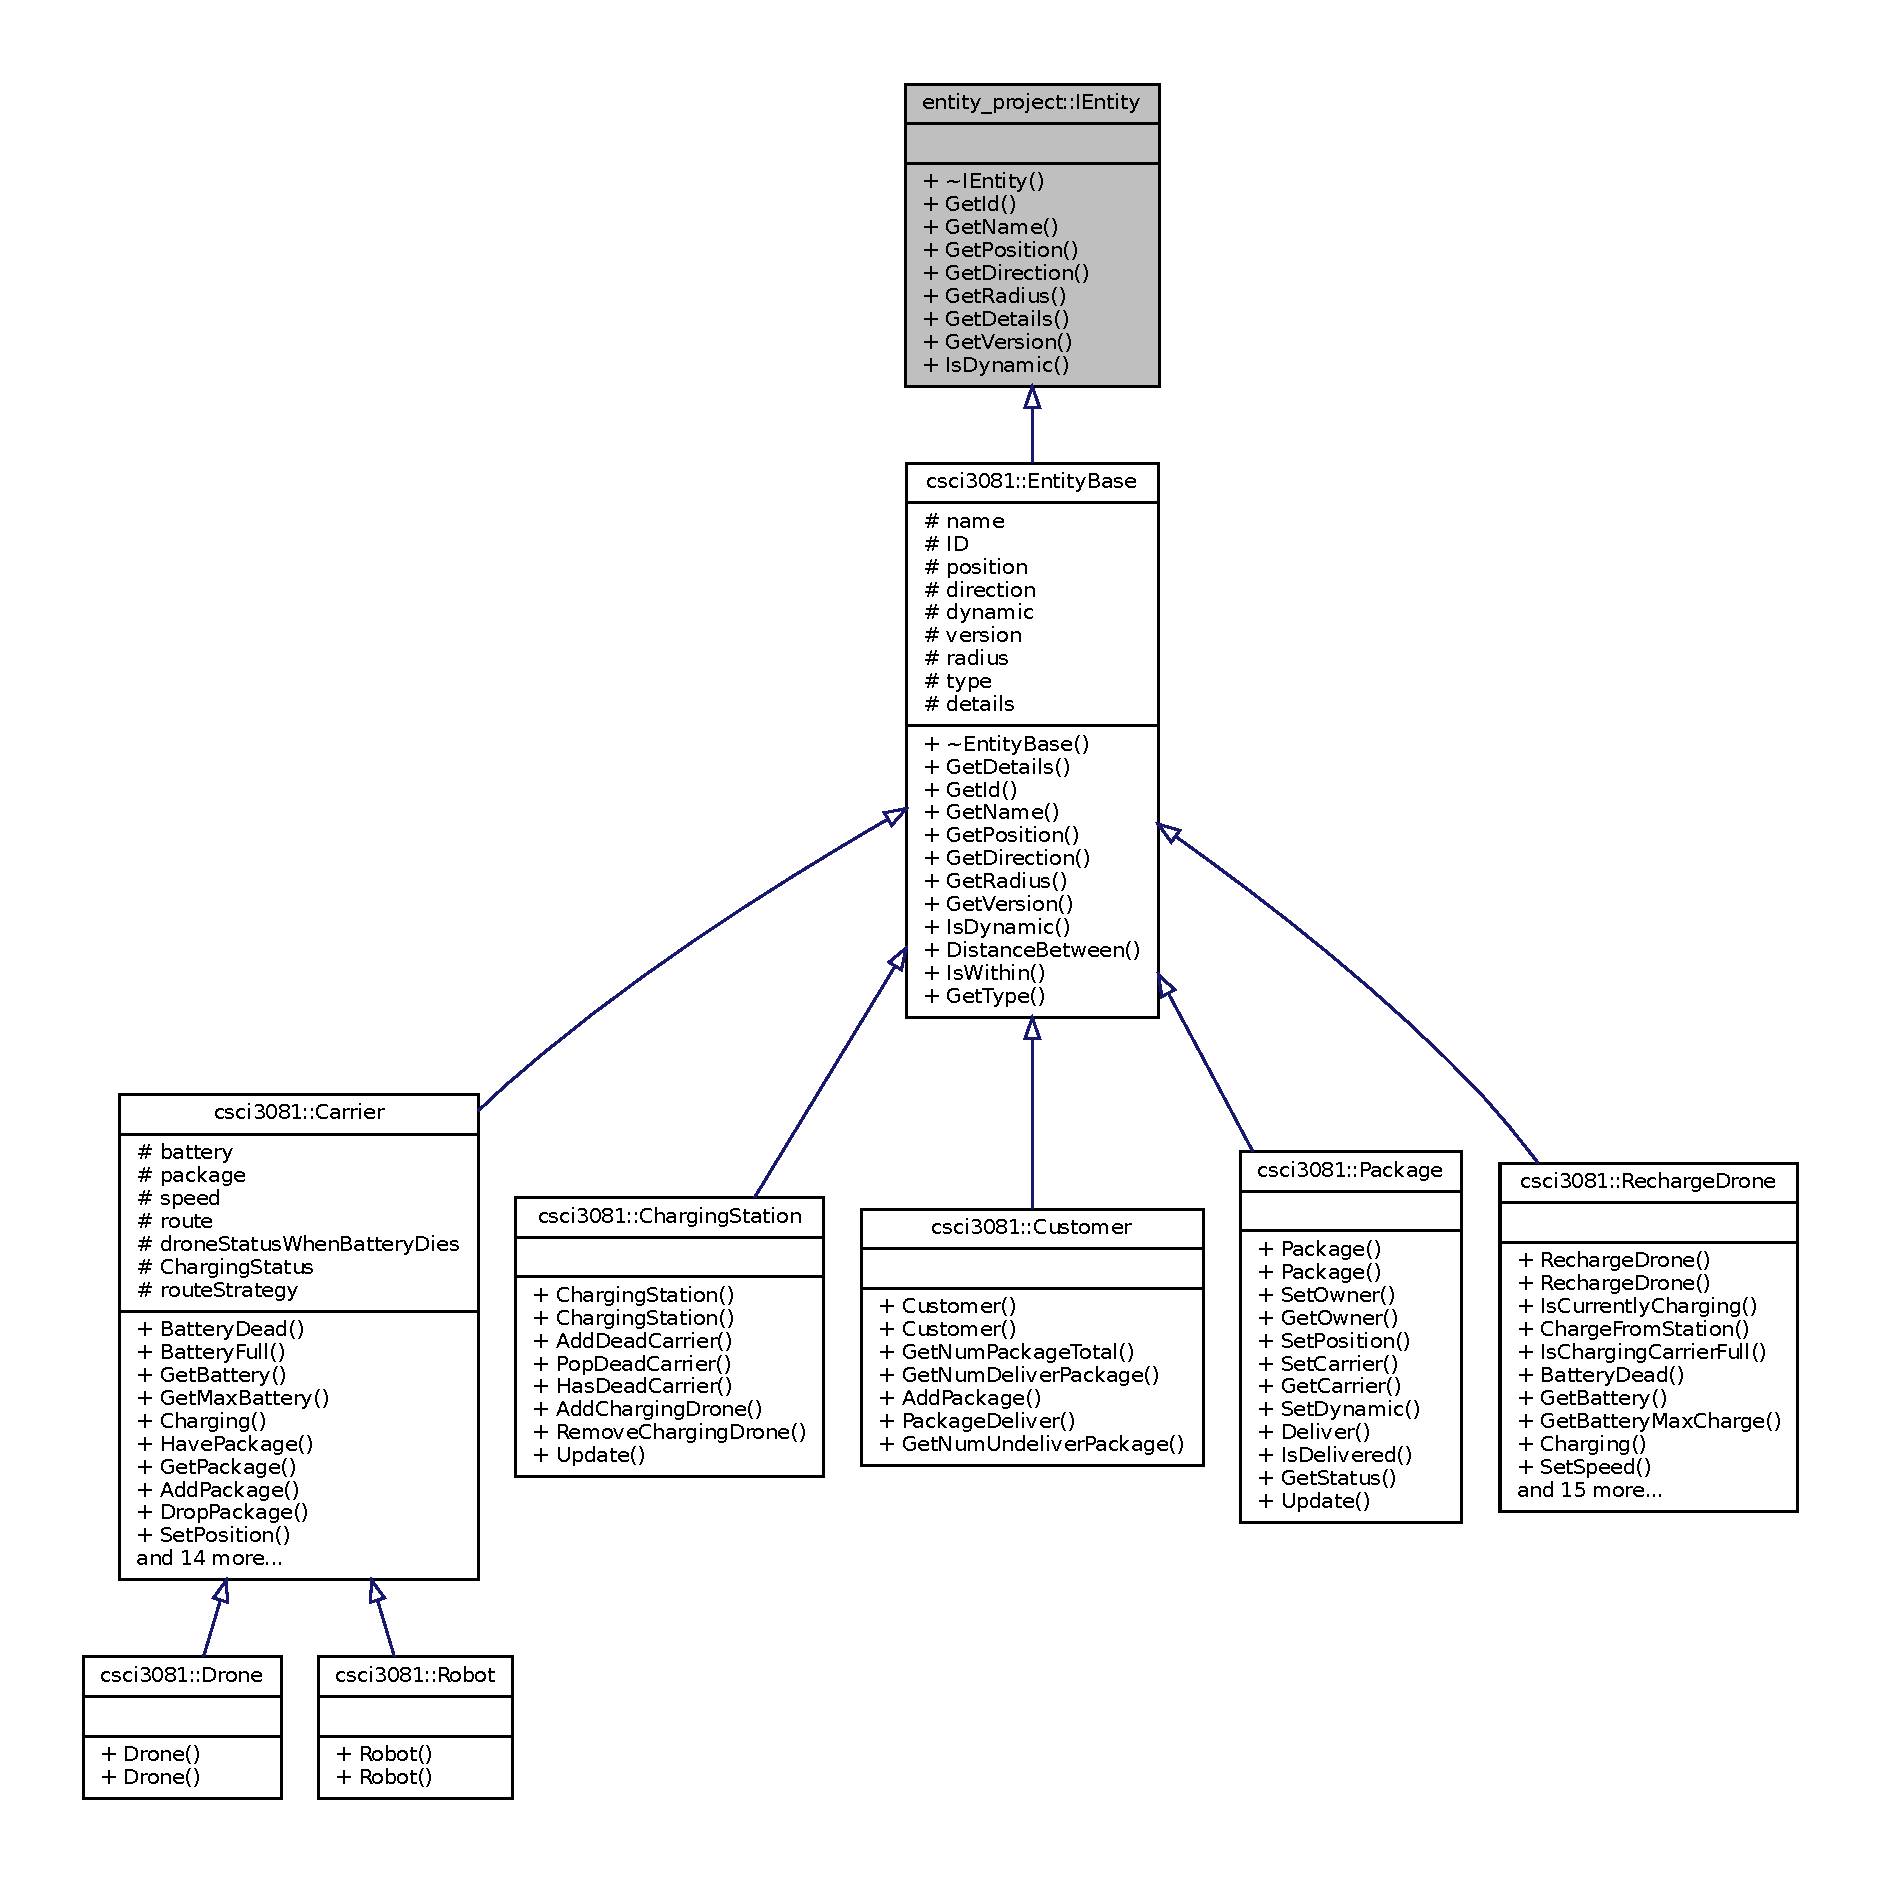
\includegraphics[width=350pt]{classentity__project_1_1IEntity__inherit__graph}
\end{center}
\end{figure}
\subsection*{Public Member Functions}
\begin{DoxyCompactItemize}
\item 
\mbox{\Hypertarget{classentity__project_1_1IEntity_a37acee64a35e2bfaccf294d20be16b7f}\label{classentity__project_1_1IEntity_a37acee64a35e2bfaccf294d20be16b7f}} 
virtual \hyperlink{classentity__project_1_1IEntity_a37acee64a35e2bfaccf294d20be16b7f}{$\sim$\+I\+Entity} ()
\begin{DoxyCompactList}\small\item\em The destructor. \end{DoxyCompactList}\item 
virtual int \hyperlink{classentity__project_1_1IEntity_a87f9d99f58cdc28b654ae9a6d82fbff6}{Get\+Id} () const =0
\item 
virtual const std\+::string \& \hyperlink{classentity__project_1_1IEntity_a60fe17f543af26a48181a0c290a822ab}{Get\+Name} ()=0
\item 
virtual const std\+::vector$<$ float $>$ \& \hyperlink{classentity__project_1_1IEntity_a1369c59d258645a12a06239ece1134cf}{Get\+Position} () const =0
\item 
virtual const std\+::vector$<$ float $>$ \& \hyperlink{classentity__project_1_1IEntity_a385dad034b5a86666df9fc979a3d1d1b}{Get\+Direction} () const =0
\item 
virtual float \hyperlink{classentity__project_1_1IEntity_af2c2f81a5d201c4c1968f055808ba59c}{Get\+Radius} () const =0
\item 
virtual const picojson\+::object \& \hyperlink{classentity__project_1_1IEntity_a73c5b6deac9e2659160d2952ae7572c4}{Get\+Details} ()=0
\item 
virtual int \hyperlink{classentity__project_1_1IEntity_a254b8c22f103ebf23261cb79bc121118}{Get\+Version} () const =0
\item 
virtual bool \hyperlink{classentity__project_1_1IEntity_a58d710abd04e533123d033a7ba80f017}{Is\+Dynamic} () const =0
\end{DoxyCompactItemize}


\subsection{Detailed Description}
A movable object in a scene. Entities have position, direction and size. 

Defines the common characteristics of an Entity.

All entities that you create must implement this interface. 

\subsection{Member Function Documentation}
\mbox{\Hypertarget{classentity__project_1_1IEntity_a73c5b6deac9e2659160d2952ae7572c4}\label{classentity__project_1_1IEntity_a73c5b6deac9e2659160d2952ae7572c4}} 
\index{entity\+\_\+project\+::\+I\+Entity@{entity\+\_\+project\+::\+I\+Entity}!Get\+Details@{Get\+Details}}
\index{Get\+Details@{Get\+Details}!entity\+\_\+project\+::\+I\+Entity@{entity\+\_\+project\+::\+I\+Entity}}
\subsubsection{\texorpdfstring{Get\+Details()}{GetDetails()}}
{\footnotesize\ttfamily virtual const picojson\+::object\& entity\+\_\+project\+::\+I\+Entity\+::\+Get\+Details (\begin{DoxyParamCaption}{ }\end{DoxyParamCaption})\hspace{0.3cm}{\ttfamily [pure virtual]}}

Returns the entity\textquotesingle{}s details. The returned picojson\+::object should be a copy of the json that was passed in when the entity was created. Details are also used to send additional information to other subsystems (e.\+g. mesh, scale, rotation, etc...). 

Implemented in \hyperlink{classcsci3081_1_1EntityBase_aed18a7db12bfc8d6908ac6c28078110c}{csci3081\+::\+Entity\+Base}.

\mbox{\Hypertarget{classentity__project_1_1IEntity_a385dad034b5a86666df9fc979a3d1d1b}\label{classentity__project_1_1IEntity_a385dad034b5a86666df9fc979a3d1d1b}} 
\index{entity\+\_\+project\+::\+I\+Entity@{entity\+\_\+project\+::\+I\+Entity}!Get\+Direction@{Get\+Direction}}
\index{Get\+Direction@{Get\+Direction}!entity\+\_\+project\+::\+I\+Entity@{entity\+\_\+project\+::\+I\+Entity}}
\subsubsection{\texorpdfstring{Get\+Direction()}{GetDirection()}}
{\footnotesize\ttfamily virtual const std\+::vector$<$float$>$\& entity\+\_\+project\+::\+I\+Entity\+::\+Get\+Direction (\begin{DoxyParamCaption}{ }\end{DoxyParamCaption}) const\hspace{0.3cm}{\ttfamily [pure virtual]}}

Returns the entity\textquotesingle{}s direction. The vector should be a unit length vector. 

Implemented in \hyperlink{classcsci3081_1_1EntityBase_aeffff43e1d9b696b0ea3de83f7bee37d}{csci3081\+::\+Entity\+Base}.

\mbox{\Hypertarget{classentity__project_1_1IEntity_a87f9d99f58cdc28b654ae9a6d82fbff6}\label{classentity__project_1_1IEntity_a87f9d99f58cdc28b654ae9a6d82fbff6}} 
\index{entity\+\_\+project\+::\+I\+Entity@{entity\+\_\+project\+::\+I\+Entity}!Get\+Id@{Get\+Id}}
\index{Get\+Id@{Get\+Id}!entity\+\_\+project\+::\+I\+Entity@{entity\+\_\+project\+::\+I\+Entity}}
\subsubsection{\texorpdfstring{Get\+Id()}{GetId()}}
{\footnotesize\ttfamily virtual int entity\+\_\+project\+::\+I\+Entity\+::\+Get\+Id (\begin{DoxyParamCaption}{ }\end{DoxyParamCaption}) const\hspace{0.3cm}{\ttfamily [pure virtual]}}

Returns the unique entity id. Each Entity should have a unique ID. 

Implemented in \hyperlink{classcsci3081_1_1EntityBase_a2802163d8d20092d985e763ad91d26da}{csci3081\+::\+Entity\+Base}.

\mbox{\Hypertarget{classentity__project_1_1IEntity_a60fe17f543af26a48181a0c290a822ab}\label{classentity__project_1_1IEntity_a60fe17f543af26a48181a0c290a822ab}} 
\index{entity\+\_\+project\+::\+I\+Entity@{entity\+\_\+project\+::\+I\+Entity}!Get\+Name@{Get\+Name}}
\index{Get\+Name@{Get\+Name}!entity\+\_\+project\+::\+I\+Entity@{entity\+\_\+project\+::\+I\+Entity}}
\subsubsection{\texorpdfstring{Get\+Name()}{GetName()}}
{\footnotesize\ttfamily virtual const std\+::string\& entity\+\_\+project\+::\+I\+Entity\+::\+Get\+Name (\begin{DoxyParamCaption}{ }\end{DoxyParamCaption})\hspace{0.3cm}{\ttfamily [pure virtual]}}

Returns the name of an entity. (Should match the \char`\"{}name\char`\"{} field of the json that was passed in when the entity was created) 

Implemented in \hyperlink{classcsci3081_1_1EntityBase_ac18421e6e96eb3939e136a579c9ac6dd}{csci3081\+::\+Entity\+Base}.

\mbox{\Hypertarget{classentity__project_1_1IEntity_a1369c59d258645a12a06239ece1134cf}\label{classentity__project_1_1IEntity_a1369c59d258645a12a06239ece1134cf}} 
\index{entity\+\_\+project\+::\+I\+Entity@{entity\+\_\+project\+::\+I\+Entity}!Get\+Position@{Get\+Position}}
\index{Get\+Position@{Get\+Position}!entity\+\_\+project\+::\+I\+Entity@{entity\+\_\+project\+::\+I\+Entity}}
\subsubsection{\texorpdfstring{Get\+Position()}{GetPosition()}}
{\footnotesize\ttfamily virtual const std\+::vector$<$float$>$\& entity\+\_\+project\+::\+I\+Entity\+::\+Get\+Position (\begin{DoxyParamCaption}{ }\end{DoxyParamCaption}) const\hspace{0.3cm}{\ttfamily [pure virtual]}}

Returns the entity\textquotesingle{}s position. The returned vector should have three values which correspond to the x, y, z, position of the entity. 

Implemented in \hyperlink{classcsci3081_1_1EntityBase_a05830db8b41c0a9c05eec08f95f683ad}{csci3081\+::\+Entity\+Base}.

\mbox{\Hypertarget{classentity__project_1_1IEntity_af2c2f81a5d201c4c1968f055808ba59c}\label{classentity__project_1_1IEntity_af2c2f81a5d201c4c1968f055808ba59c}} 
\index{entity\+\_\+project\+::\+I\+Entity@{entity\+\_\+project\+::\+I\+Entity}!Get\+Radius@{Get\+Radius}}
\index{Get\+Radius@{Get\+Radius}!entity\+\_\+project\+::\+I\+Entity@{entity\+\_\+project\+::\+I\+Entity}}
\subsubsection{\texorpdfstring{Get\+Radius()}{GetRadius()}}
{\footnotesize\ttfamily virtual float entity\+\_\+project\+::\+I\+Entity\+::\+Get\+Radius (\begin{DoxyParamCaption}{ }\end{DoxyParamCaption}) const\hspace{0.3cm}{\ttfamily [pure virtual]}}

Returns the entity\textquotesingle{}s radius. Entities are bounded by a sphere used for calculating proximity to boundaries or other entities. 

Implemented in \hyperlink{classcsci3081_1_1EntityBase_abf61eb1cc8b94a7756f0ebc6a0c8a8f3}{csci3081\+::\+Entity\+Base}.

\mbox{\Hypertarget{classentity__project_1_1IEntity_a254b8c22f103ebf23261cb79bc121118}\label{classentity__project_1_1IEntity_a254b8c22f103ebf23261cb79bc121118}} 
\index{entity\+\_\+project\+::\+I\+Entity@{entity\+\_\+project\+::\+I\+Entity}!Get\+Version@{Get\+Version}}
\index{Get\+Version@{Get\+Version}!entity\+\_\+project\+::\+I\+Entity@{entity\+\_\+project\+::\+I\+Entity}}
\subsubsection{\texorpdfstring{Get\+Version()}{GetVersion()}}
{\footnotesize\ttfamily virtual int entity\+\_\+project\+::\+I\+Entity\+::\+Get\+Version (\begin{DoxyParamCaption}{ }\end{DoxyParamCaption}) const\hspace{0.3cm}{\ttfamily [pure virtual]}}

Get version can be used to see whether or not a variable other than position or direction has changed. 

Implemented in \hyperlink{classcsci3081_1_1EntityBase_af5c87e8daf9161dc8c959c355b076bea}{csci3081\+::\+Entity\+Base}.

\mbox{\Hypertarget{classentity__project_1_1IEntity_a58d710abd04e533123d033a7ba80f017}\label{classentity__project_1_1IEntity_a58d710abd04e533123d033a7ba80f017}} 
\index{entity\+\_\+project\+::\+I\+Entity@{entity\+\_\+project\+::\+I\+Entity}!Is\+Dynamic@{Is\+Dynamic}}
\index{Is\+Dynamic@{Is\+Dynamic}!entity\+\_\+project\+::\+I\+Entity@{entity\+\_\+project\+::\+I\+Entity}}
\subsubsection{\texorpdfstring{Is\+Dynamic()}{IsDynamic()}}
{\footnotesize\ttfamily virtual bool entity\+\_\+project\+::\+I\+Entity\+::\+Is\+Dynamic (\begin{DoxyParamCaption}{ }\end{DoxyParamCaption}) const\hspace{0.3cm}{\ttfamily [pure virtual]}}

This method specifies whether or not the entity is static (doesn\textquotesingle{}t change) or moves. It should return true if you want the entities position/orientation to be updated in the visualization.

Combining \hyperlink{classentity__project_1_1IEntity_a254b8c22f103ebf23261cb79bc121118}{Get\+Version()} with a non-\/dynamic entity allows the entity to be updated less often than on a frame by frame basis for other subsystems. For example, we may want to update a dynamic object every frame, while it is more efficient to update a static object only when the version changes. 

Implemented in \hyperlink{classcsci3081_1_1EntityBase_aa2a894f7821745acd91fbfb2e2e92082}{csci3081\+::\+Entity\+Base}.



The documentation for this class was generated from the following file\+:\begin{DoxyCompactItemize}
\item 
/home/user/repo/.\+dependencies/include/\+Entity\+Project/entity.\+h\end{DoxyCompactItemize}

\hypertarget{classentity__project_1_1IEntityFactory}{}\section{entity\+\_\+project\+:\+:I\+Entity\+Factory Class Reference}
\label{classentity__project_1_1IEntityFactory}\index{entity\+\_\+project\+::\+I\+Entity\+Factory@{entity\+\_\+project\+::\+I\+Entity\+Factory}}


{\ttfamily \#include $<$entity\+\_\+factory.\+h$>$}



Inheritance diagram for entity\+\_\+project\+:\+:I\+Entity\+Factory\+:
\nopagebreak
\begin{figure}[H]
\begin{center}
\leavevmode
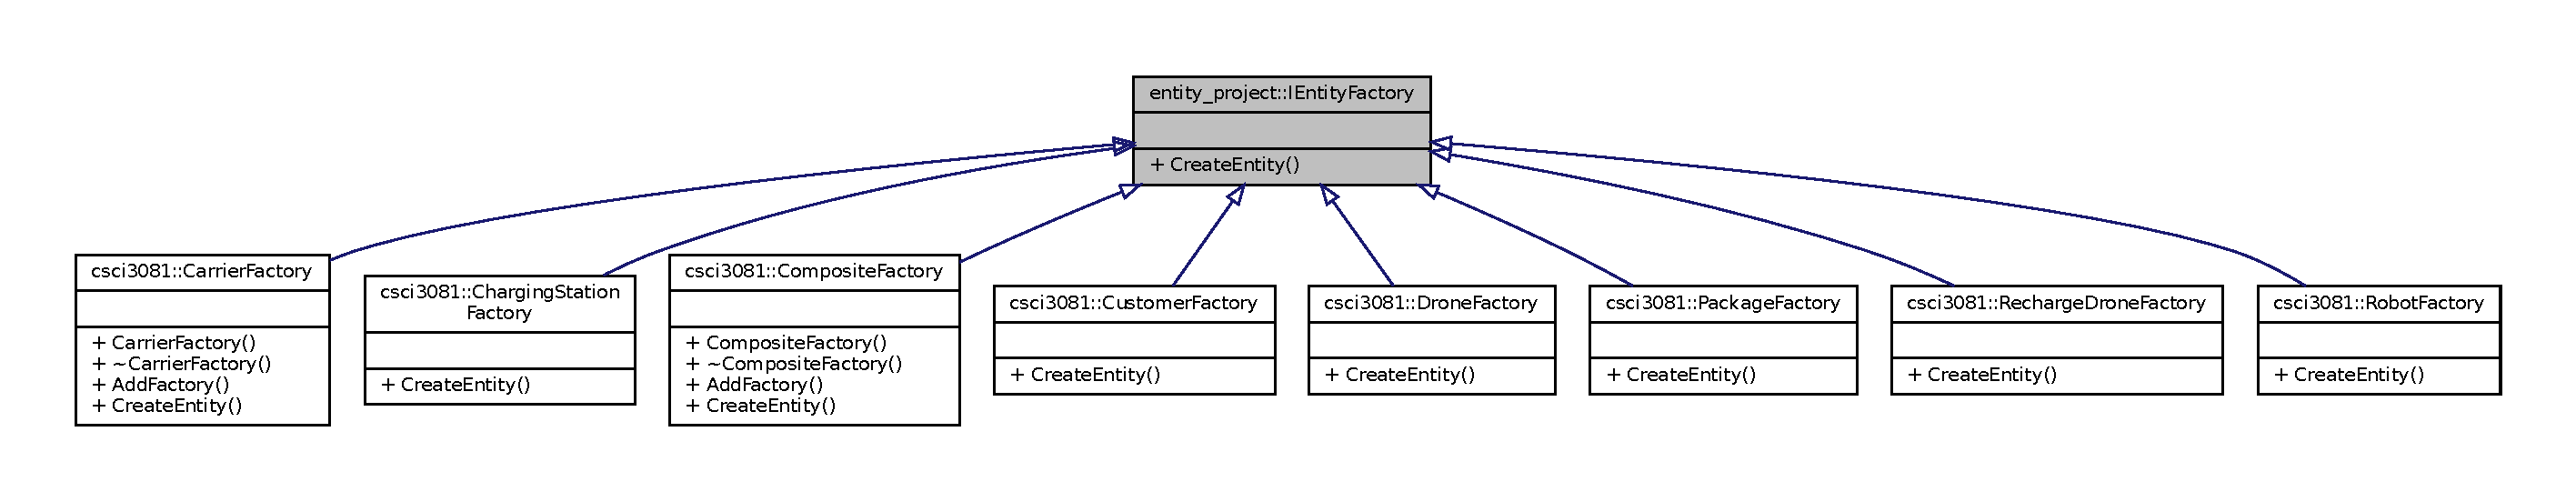
\includegraphics[width=350pt]{classentity__project_1_1IEntityFactory__inherit__graph}
\end{center}
\end{figure}
\subsection*{Public Member Functions}
\begin{DoxyCompactItemize}
\item 
\mbox{\Hypertarget{classentity__project_1_1IEntityFactory_ac4e8eaf4294958fef0b98bd3684704bb}\label{classentity__project_1_1IEntityFactory_ac4e8eaf4294958fef0b98bd3684704bb}} 
virtual \hyperlink{classentity__project_1_1IEntity}{I\+Entity} $\ast$ \hyperlink{classentity__project_1_1IEntityFactory_ac4e8eaf4294958fef0b98bd3684704bb}{Create\+Entity} (const picojson\+::object \&val)=0
\begin{DoxyCompactList}\small\item\em returns a pointer to a newly created entity \end{DoxyCompactList}\end{DoxyCompactItemize}


\subsection{Detailed Description}
U\+S\+A\+GE\+: This class is meant to be inhereted by your own entity factory classes Implement this class to manage the creation of entity objects in your system. 

The documentation for this class was generated from the following file\+:\begin{DoxyCompactItemize}
\item 
/home/user/repo/.\+dependencies/include/\+Entity\+Project/entity\+\_\+factory.\+h\end{DoxyCompactItemize}

\hypertarget{classentity__project_1_1IEntityObserver}{}\section{entity\+\_\+project\+:\+:I\+Entity\+Observer Class Reference}
\label{classentity__project_1_1IEntityObserver}\index{entity\+\_\+project\+::\+I\+Entity\+Observer@{entity\+\_\+project\+::\+I\+Entity\+Observer}}


Observers entity events when they occur.  




{\ttfamily \#include $<$entity\+\_\+observer.\+h$>$}



Inheritance diagram for entity\+\_\+project\+:\+:I\+Entity\+Observer\+:
\nopagebreak
\begin{figure}[H]
\begin{center}
\leavevmode
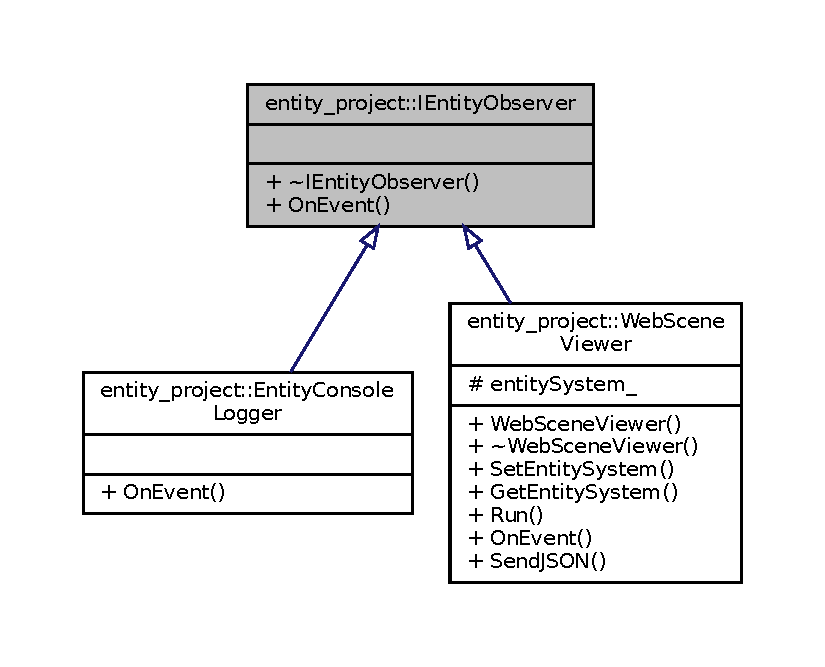
\includegraphics[width=350pt]{classentity__project_1_1IEntityObserver__inherit__graph}
\end{center}
\end{figure}
\subsection*{Public Member Functions}
\begin{DoxyCompactItemize}
\item 
\mbox{\Hypertarget{classentity__project_1_1IEntityObserver_acafdf6ac59d9522d4d08cdfb52dec8d4}\label{classentity__project_1_1IEntityObserver_acafdf6ac59d9522d4d08cdfb52dec8d4}} 
virtual \hyperlink{classentity__project_1_1IEntityObserver_acafdf6ac59d9522d4d08cdfb52dec8d4}{$\sim$\+I\+Entity\+Observer} ()
\begin{DoxyCompactList}\small\item\em Destructor. \end{DoxyCompactList}\item 
\mbox{\Hypertarget{classentity__project_1_1IEntityObserver_ac346f41c002c1f7cd4aa4ee501146c6c}\label{classentity__project_1_1IEntityObserver_ac346f41c002c1f7cd4aa4ee501146c6c}} 
virtual void \hyperlink{classentity__project_1_1IEntityObserver_ac346f41c002c1f7cd4aa4ee501146c6c}{On\+Event} (const picojson\+::value \&event, const \hyperlink{classentity__project_1_1IEntity}{I\+Entity} \&entity)=0
\begin{DoxyCompactList}\small\item\em Callback when an event happens. \end{DoxyCompactList}\end{DoxyCompactItemize}


\subsection{Detailed Description}
Observers entity events when they occur. 

U\+S\+A\+GE\+: This class is meant to be inhereted by your own entity observer class This class is available in order to enable the observer pattern for entities. A callback function on\+Event 

The documentation for this class was generated from the following file\+:\begin{DoxyCompactItemize}
\item 
/home/user/repo/.\+dependencies/include/\+Entity\+Project/entity\+\_\+observer.\+h\end{DoxyCompactItemize}

\hypertarget{classentity__project_1_1IEntitySystem}{}\section{entity\+\_\+project\+:\+:I\+Entity\+System Class Reference}
\label{classentity__project_1_1IEntitySystem}\index{entity\+\_\+project\+::\+I\+Entity\+System@{entity\+\_\+project\+::\+I\+Entity\+System}}


An abstract class that represents an entity system that contains entities and updates over time.  




{\ttfamily \#include $<$entity\+\_\+system.\+h$>$}



Inheritance diagram for entity\+\_\+project\+:\+:I\+Entity\+System\+:
\nopagebreak
\begin{figure}[H]
\begin{center}
\leavevmode
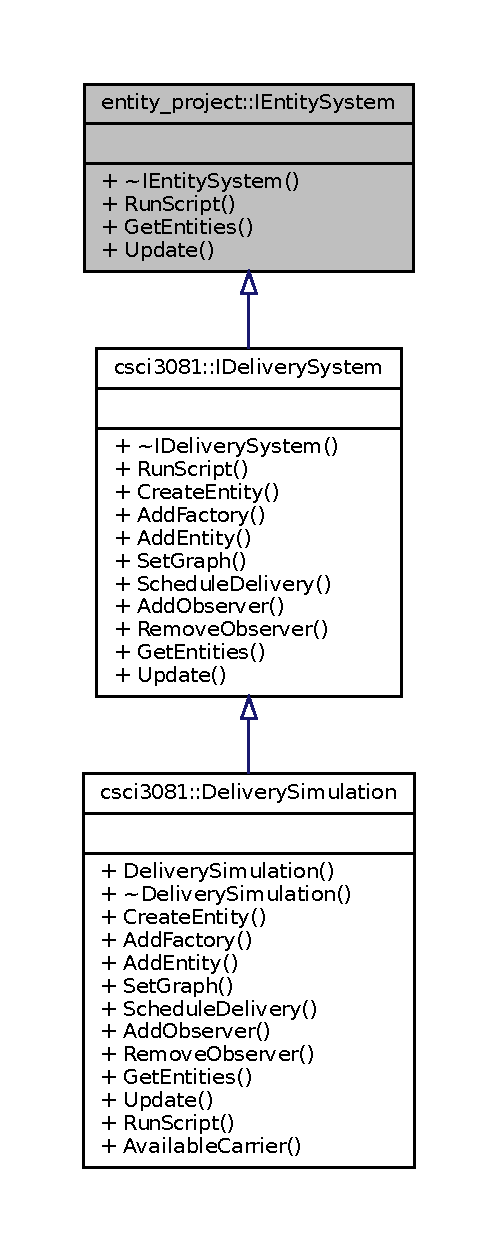
\includegraphics[height=550pt]{classentity__project_1_1IEntitySystem__inherit__graph}
\end{center}
\end{figure}
\subsection*{Public Member Functions}
\begin{DoxyCompactItemize}
\item 
\mbox{\Hypertarget{classentity__project_1_1IEntitySystem_ab4ba3624f6f8c76b6040874dad2f9e6f}\label{classentity__project_1_1IEntitySystem_ab4ba3624f6f8c76b6040874dad2f9e6f}} 
virtual \hyperlink{classentity__project_1_1IEntitySystem_ab4ba3624f6f8c76b6040874dad2f9e6f}{$\sim$\+I\+Entity\+System} ()
\begin{DoxyCompactList}\small\item\em Destructor. \end{DoxyCompactList}\item 
virtual void \hyperlink{classentity__project_1_1IEntitySystem_a57a31878f9ae43f2ac3e70aa1903b8ec}{Run\+Script} (const picojson\+::array \&script, \hyperlink{classentity__project_1_1IEntitySystem}{I\+Entity\+System} $\ast$system) const =0
\begin{DoxyCompactList}\small\item\em Runs a J\+S\+ON script on an entity system as a set of commands. \end{DoxyCompactList}\item 
\mbox{\Hypertarget{classentity__project_1_1IEntitySystem_a43255ef96f8504e2a536d10fd018e52a}\label{classentity__project_1_1IEntitySystem_a43255ef96f8504e2a536d10fd018e52a}} 
virtual const std\+::vector$<$ \hyperlink{classentity__project_1_1IEntity}{I\+Entity} $\ast$ $>$ \& \hyperlink{classentity__project_1_1IEntitySystem_a43255ef96f8504e2a536d10fd018e52a}{Get\+Entities} () const =0
\begin{DoxyCompactList}\small\item\em Returns the list of entities in the system. \end{DoxyCompactList}\item 
\mbox{\Hypertarget{classentity__project_1_1IEntitySystem_ada758b54da573bb18372880633544c20}\label{classentity__project_1_1IEntitySystem_ada758b54da573bb18372880633544c20}} 
virtual void \hyperlink{classentity__project_1_1IEntitySystem_ada758b54da573bb18372880633544c20}{Update} (float dt)=0
\begin{DoxyCompactList}\small\item\em Updates the entity system by a time of dt. \end{DoxyCompactList}\end{DoxyCompactItemize}


\subsection{Detailed Description}
An abstract class that represents an entity system that contains entities and updates over time. 

\subsection{Member Function Documentation}
\mbox{\Hypertarget{classentity__project_1_1IEntitySystem_a57a31878f9ae43f2ac3e70aa1903b8ec}\label{classentity__project_1_1IEntitySystem_a57a31878f9ae43f2ac3e70aa1903b8ec}} 
\index{entity\+\_\+project\+::\+I\+Entity\+System@{entity\+\_\+project\+::\+I\+Entity\+System}!Run\+Script@{Run\+Script}}
\index{Run\+Script@{Run\+Script}!entity\+\_\+project\+::\+I\+Entity\+System@{entity\+\_\+project\+::\+I\+Entity\+System}}
\subsubsection{\texorpdfstring{Run\+Script()}{RunScript()}}
{\footnotesize\ttfamily virtual void entity\+\_\+project\+::\+I\+Entity\+System\+::\+Run\+Script (\begin{DoxyParamCaption}\item[{const picojson\+::array \&}]{script,  }\item[{\hyperlink{classentity__project_1_1IEntitySystem}{I\+Entity\+System} $\ast$}]{system }\end{DoxyParamCaption}) const\hspace{0.3cm}{\ttfamily [pure virtual]}}



Runs a J\+S\+ON script on an entity system as a set of commands. 

This method does not make any changes to the current entity system, but rather acts as a strategy for the entity system passed into the method. It is therefore possible to override how scripts are read in depending on the application. 

Implemented in \hyperlink{classcsci3081_1_1DeliverySimulation_a332938cb4b972af169ad58dbc1b3bb05}{csci3081\+::\+Delivery\+Simulation}, and \hyperlink{classcsci3081_1_1IDeliverySystem_ae152276130e859b052f1d89417be6fc2}{csci3081\+::\+I\+Delivery\+System}.



The documentation for this class was generated from the following file\+:\begin{DoxyCompactItemize}
\item 
/home/user/repo/.\+dependencies/include/\+Entity\+Project/entity\+\_\+system.\+h\end{DoxyCompactItemize}

\hypertarget{classentity__project_1_1IGraph}{}\section{entity\+\_\+project\+:\+:I\+Graph Class Reference}
\label{classentity__project_1_1IGraph}\index{entity\+\_\+project\+::\+I\+Graph@{entity\+\_\+project\+::\+I\+Graph}}


Represents a read only graph object.  




{\ttfamily \#include $<$graph.\+h$>$}

\subsection*{Public Member Functions}
\begin{DoxyCompactItemize}
\item 
\mbox{\Hypertarget{classentity__project_1_1IGraph_ad4eafcdb3b6902e54924a6c21e1971a0}\label{classentity__project_1_1IGraph_ad4eafcdb3b6902e54924a6c21e1971a0}} 
virtual \hyperlink{classentity__project_1_1IGraph_ad4eafcdb3b6902e54924a6c21e1971a0}{$\sim$\+I\+Graph} ()
\begin{DoxyCompactList}\small\item\em Destructor. \end{DoxyCompactList}\item 
\mbox{\Hypertarget{classentity__project_1_1IGraph_a900c64b856e9163727693276fc870bd9}\label{classentity__project_1_1IGraph_a900c64b856e9163727693276fc870bd9}} 
virtual const \hyperlink{classentity__project_1_1IGraphNode}{I\+Graph\+Node} $\ast$ \hyperlink{classentity__project_1_1IGraph_a900c64b856e9163727693276fc870bd9}{Get\+Node} (const std\+::string \&name) const =0
\begin{DoxyCompactList}\small\item\em Gets a node in the graph by name. \end{DoxyCompactList}\item 
\mbox{\Hypertarget{classentity__project_1_1IGraph_a690ed9b025c9b7709154c4fc7f89ef93}\label{classentity__project_1_1IGraph_a690ed9b025c9b7709154c4fc7f89ef93}} 
virtual const std\+::vector$<$ \hyperlink{classentity__project_1_1IGraphNode}{I\+Graph\+Node} $\ast$ $>$ \& \hyperlink{classentity__project_1_1IGraph_a690ed9b025c9b7709154c4fc7f89ef93}{Get\+Nodes} () const =0
\begin{DoxyCompactList}\small\item\em Gets all nodes in the graph. \end{DoxyCompactList}\item 
virtual const std\+::vector$<$ std\+::vector$<$ float $>$ $>$ \hyperlink{classentity__project_1_1IGraph_aa96a691b82108d0901463f3cd5cd79b9}{Get\+Path} (std\+::vector$<$ float $>$ src, std\+::vector$<$ float $>$ dest) const =0
\begin{DoxyCompactList}\small\item\em Returns a vector of float vectors that represent a path from src to dest. \end{DoxyCompactList}\end{DoxyCompactItemize}


\subsection{Detailed Description}
Represents a read only graph object. 

\subsection{Member Function Documentation}
\mbox{\Hypertarget{classentity__project_1_1IGraph_aa96a691b82108d0901463f3cd5cd79b9}\label{classentity__project_1_1IGraph_aa96a691b82108d0901463f3cd5cd79b9}} 
\index{entity\+\_\+project\+::\+I\+Graph@{entity\+\_\+project\+::\+I\+Graph}!Get\+Path@{Get\+Path}}
\index{Get\+Path@{Get\+Path}!entity\+\_\+project\+::\+I\+Graph@{entity\+\_\+project\+::\+I\+Graph}}
\subsubsection{\texorpdfstring{Get\+Path()}{GetPath()}}
{\footnotesize\ttfamily virtual const std\+::vector$<$ std\+::vector$<$float$>$ $>$ entity\+\_\+project\+::\+I\+Graph\+::\+Get\+Path (\begin{DoxyParamCaption}\item[{std\+::vector$<$ float $>$}]{src,  }\item[{std\+::vector$<$ float $>$}]{dest }\end{DoxyParamCaption}) const\hspace{0.3cm}{\ttfamily [pure virtual]}}



Returns a vector of float vectors that represent a path from src to dest. 

Given a source and destination in the form of 3-\/element x,y,z vectors, this function will return a list of positions to traverse in-\/order, which avoids the geometry of the scene. The returned path includes the source and destination points. 

The documentation for this class was generated from the following file\+:\begin{DoxyCompactItemize}
\item 
/home/user/repo/.\+dependencies/include/\+Entity\+Project/graph.\+h\end{DoxyCompactItemize}

\hypertarget{classentity__project_1_1IGraphNode}{}\section{entity\+\_\+project\+:\+:I\+Graph\+Node Class Reference}
\label{classentity__project_1_1IGraphNode}\index{entity\+\_\+project\+::\+I\+Graph\+Node@{entity\+\_\+project\+::\+I\+Graph\+Node}}


Represents a node in a graph object.  




{\ttfamily \#include $<$graph.\+h$>$}

\subsection*{Public Member Functions}
\begin{DoxyCompactItemize}
\item 
\mbox{\Hypertarget{classentity__project_1_1IGraphNode_ab77a03adc593f292be5d2e55fdbbbfa0}\label{classentity__project_1_1IGraphNode_ab77a03adc593f292be5d2e55fdbbbfa0}} 
virtual \hyperlink{classentity__project_1_1IGraphNode_ab77a03adc593f292be5d2e55fdbbbfa0}{$\sim$\+I\+Graph\+Node} ()
\begin{DoxyCompactList}\small\item\em Destructor. \end{DoxyCompactList}\item 
\mbox{\Hypertarget{classentity__project_1_1IGraphNode_a05cdf42e5c6a3040017a1c8f5acdd25c}\label{classentity__project_1_1IGraphNode_a05cdf42e5c6a3040017a1c8f5acdd25c}} 
virtual const std\+::string \& \hyperlink{classentity__project_1_1IGraphNode_a05cdf42e5c6a3040017a1c8f5acdd25c}{Get\+Name} () const =0
\begin{DoxyCompactList}\small\item\em Gets the node name. \end{DoxyCompactList}\item 
\mbox{\Hypertarget{classentity__project_1_1IGraphNode_a382babc90ffbef731485f9116d605204}\label{classentity__project_1_1IGraphNode_a382babc90ffbef731485f9116d605204}} 
virtual const std\+::vector$<$ \hyperlink{classentity__project_1_1IGraphNode}{I\+Graph\+Node} $\ast$ $>$ \& \hyperlink{classentity__project_1_1IGraphNode_a382babc90ffbef731485f9116d605204}{Get\+Neighbors} () const =0
\begin{DoxyCompactList}\small\item\em Gets the node\textquotesingle{}s neighbors. \end{DoxyCompactList}\item 
\mbox{\Hypertarget{classentity__project_1_1IGraphNode_ad95b25e4a3285c7ba36a6ecc9ad2df9f}\label{classentity__project_1_1IGraphNode_ad95b25e4a3285c7ba36a6ecc9ad2df9f}} 
virtual const std\+::vector$<$ float $>$ \hyperlink{classentity__project_1_1IGraphNode_ad95b25e4a3285c7ba36a6ecc9ad2df9f}{Get\+Position} () const =0
\begin{DoxyCompactList}\small\item\em Gets the node\textquotesingle{}s position. \end{DoxyCompactList}\end{DoxyCompactItemize}


\subsection{Detailed Description}
Represents a node in a graph object. 

The documentation for this class was generated from the following file\+:\begin{DoxyCompactItemize}
\item 
/home/user/repo/.\+dependencies/include/\+Entity\+Project/graph.\+h\end{DoxyCompactItemize}

\hypertarget{classentity__project_1_1ISceneViewer}{}\section{entity\+\_\+project\+:\+:I\+Scene\+Viewer Class Reference}
\label{classentity__project_1_1ISceneViewer}\index{entity\+\_\+project\+::\+I\+Scene\+Viewer@{entity\+\_\+project\+::\+I\+Scene\+Viewer}}


Abstact class for viewing a scene representing an entity system.  




{\ttfamily \#include $<$scene\+\_\+viewer.\+h$>$}



Inheritance diagram for entity\+\_\+project\+:\+:I\+Scene\+Viewer\+:
\nopagebreak
\begin{figure}[H]
\begin{center}
\leavevmode
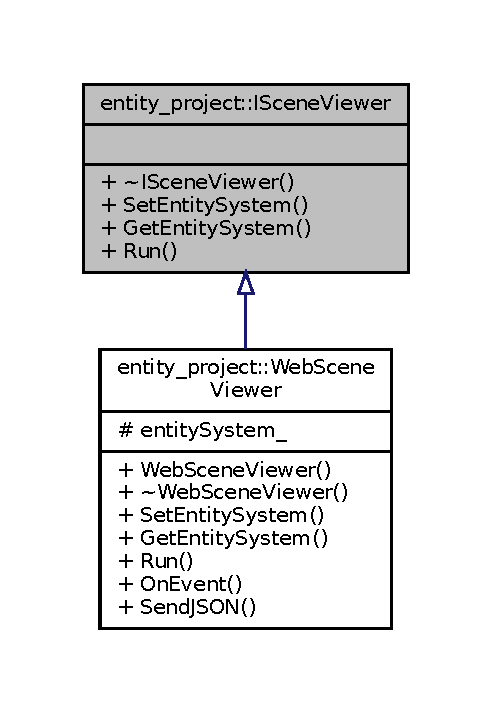
\includegraphics[width=236pt]{classentity__project_1_1ISceneViewer__inherit__graph}
\end{center}
\end{figure}
\subsection*{Public Member Functions}
\begin{DoxyCompactItemize}
\item 
\mbox{\Hypertarget{classentity__project_1_1ISceneViewer_a5ce3bce5d4764098ec8db47ecd5e4780}\label{classentity__project_1_1ISceneViewer_a5ce3bce5d4764098ec8db47ecd5e4780}} 
virtual \hyperlink{classentity__project_1_1ISceneViewer_a5ce3bce5d4764098ec8db47ecd5e4780}{$\sim$\+I\+Scene\+Viewer} ()
\begin{DoxyCompactList}\small\item\em Destructor. \end{DoxyCompactList}\item 
\mbox{\Hypertarget{classentity__project_1_1ISceneViewer_ab6c9ee1c8c551dd463e8ff1788b3d407}\label{classentity__project_1_1ISceneViewer_ab6c9ee1c8c551dd463e8ff1788b3d407}} 
virtual void \hyperlink{classentity__project_1_1ISceneViewer_ab6c9ee1c8c551dd463e8ff1788b3d407}{Set\+Entity\+System} (\hyperlink{classentity__project_1_1IEntitySystem}{I\+Entity\+System} $\ast$entity\+System)=0
\begin{DoxyCompactList}\small\item\em Sets the current entity system model that the viewer visualizes. \end{DoxyCompactList}\item 
\mbox{\Hypertarget{classentity__project_1_1ISceneViewer_a1ed816d97624174d415403c3206fa1b6}\label{classentity__project_1_1ISceneViewer_a1ed816d97624174d415403c3206fa1b6}} 
virtual \hyperlink{classentity__project_1_1IEntitySystem}{I\+Entity\+System} $\ast$ \hyperlink{classentity__project_1_1ISceneViewer_a1ed816d97624174d415403c3206fa1b6}{Get\+Entity\+System} () const =0
\begin{DoxyCompactList}\small\item\em Returns the current entity system. \end{DoxyCompactList}\item 
\mbox{\Hypertarget{classentity__project_1_1ISceneViewer_a247a0ab155d8fefcbcae2dbb1685ff7f}\label{classentity__project_1_1ISceneViewer_a247a0ab155d8fefcbcae2dbb1685ff7f}} 
virtual bool \hyperlink{classentity__project_1_1ISceneViewer_a247a0ab155d8fefcbcae2dbb1685ff7f}{Run} ()=0
\begin{DoxyCompactList}\small\item\em Runs the visualization. \end{DoxyCompactList}\end{DoxyCompactItemize}


\subsection{Detailed Description}
Abstact class for viewing a scene representing an entity system. 

Overide this class for different types of viewers. 

The documentation for this class was generated from the following file\+:\begin{DoxyCompactItemize}
\item 
/home/user/repo/.\+dependencies/include/\+Entity\+Project/scene\+\_\+viewer.\+h\end{DoxyCompactItemize}

\hypertarget{classcsci3081_1_1JsonHelper}{}\section{csci3081\+:\+:Json\+Helper Class Reference}
\label{classcsci3081_1_1JsonHelper}\index{csci3081\+::\+Json\+Helper@{csci3081\+::\+Json\+Helper}}
\subsection*{Static Public Member Functions}
\begin{DoxyCompactItemize}
\item 
static const picojson\+::value \& \hyperlink{classcsci3081_1_1JsonHelper_a5c690dab7594cc0a33e6c17cf7afc708}{Get\+Value} (const picojson\+::object \&obj, std\+::string key)
\begin{DoxyCompactList}\small\item\em Returns the key from json object obj as a json value, throws error if key doesn\textquotesingle{}t exist. \end{DoxyCompactList}\item 
\mbox{\Hypertarget{classcsci3081_1_1JsonHelper_ae11653e9550cf64a42e531aa03593307}\label{classcsci3081_1_1JsonHelper_ae11653e9550cf64a42e531aa03593307}} 
static const picojson\+::object \& \hyperlink{classcsci3081_1_1JsonHelper_ae11653e9550cf64a42e531aa03593307}{Get\+Object} (const picojson\+::object \&obj, std\+::string key)
\begin{DoxyCompactList}\small\item\em Returns the key from json object obj as a json object, throws error if key doesn\textquotesingle{}t exist. \end{DoxyCompactList}\item 
\mbox{\Hypertarget{classcsci3081_1_1JsonHelper_afd99b2ed07c187ca1fa2f95adc5d1346}\label{classcsci3081_1_1JsonHelper_afd99b2ed07c187ca1fa2f95adc5d1346}} 
static const picojson\+::array \& \hyperlink{classcsci3081_1_1JsonHelper_afd99b2ed07c187ca1fa2f95adc5d1346}{Get\+Array} (const picojson\+::object \&obj, std\+::string key)
\begin{DoxyCompactList}\small\item\em Returns the key from json object obj as a json array, will throw an error if key doesn\textquotesingle{}t exist. \end{DoxyCompactList}\item 
\mbox{\Hypertarget{classcsci3081_1_1JsonHelper_af50a46a1f75f23c755e45b8477f69133}\label{classcsci3081_1_1JsonHelper_af50a46a1f75f23c755e45b8477f69133}} 
static std\+::string \hyperlink{classcsci3081_1_1JsonHelper_af50a46a1f75f23c755e45b8477f69133}{Get\+String} (const picojson\+::object \&obj, std\+::string key)
\begin{DoxyCompactList}\small\item\em Returns the key from json object obj as a string, will throw an error if key doesn\textquotesingle{}t exist. \end{DoxyCompactList}\item 
\mbox{\Hypertarget{classcsci3081_1_1JsonHelper_ae190f5c7e182d60c52d6b9e06dc97def}\label{classcsci3081_1_1JsonHelper_ae190f5c7e182d60c52d6b9e06dc97def}} 
static double \hyperlink{classcsci3081_1_1JsonHelper_ae190f5c7e182d60c52d6b9e06dc97def}{Get\+Double} (const picojson\+::object \&obj, std\+::string key)
\begin{DoxyCompactList}\small\item\em Returns the key from json object obj as a double, will throw an error if key doesn\textquotesingle{}t exist. \end{DoxyCompactList}\item 
\mbox{\Hypertarget{classcsci3081_1_1JsonHelper_a0c243724051e5fb795c40701d66d844e}\label{classcsci3081_1_1JsonHelper_a0c243724051e5fb795c40701d66d844e}} 
static std\+::vector$<$ float $>$ \hyperlink{classcsci3081_1_1JsonHelper_a0c243724051e5fb795c40701d66d844e}{Get\+Std\+Float\+Vector} (const picojson\+::object \&obj, std\+::string key)
\begin{DoxyCompactList}\small\item\em Returns the key from json object obj as a float vector, will throw an error if key doesn\textquotesingle{}t exist. \end{DoxyCompactList}\item 
\mbox{\Hypertarget{classcsci3081_1_1JsonHelper_acb0d4fa20d41a93d4076b447d732d0fa}\label{classcsci3081_1_1JsonHelper_acb0d4fa20d41a93d4076b447d732d0fa}} 
static bool \hyperlink{classcsci3081_1_1JsonHelper_acb0d4fa20d41a93d4076b447d732d0fa}{Contains\+Key} (const picojson\+::object \&obj, std\+::string key)
\begin{DoxyCompactList}\small\item\em Returns a boolean value of whether the json object obj contains key or not. \end{DoxyCompactList}\item 
\mbox{\Hypertarget{classcsci3081_1_1JsonHelper_a5a69da28dbe3017826d53bdc6d17652f}\label{classcsci3081_1_1JsonHelper_a5a69da28dbe3017826d53bdc6d17652f}} 
static picojson\+::object \hyperlink{classcsci3081_1_1JsonHelper_a5a69da28dbe3017826d53bdc6d17652f}{Create\+Json\+Notification} ()
\begin{DoxyCompactList}\small\item\em Create a new json object for sending notifications. \end{DoxyCompactList}\item 
\mbox{\Hypertarget{classcsci3081_1_1JsonHelper_a58c0b129bcdd4f4fcbab655a47ab7a2b}\label{classcsci3081_1_1JsonHelper_a58c0b129bcdd4f4fcbab655a47ab7a2b}} 
static picojson\+::object \hyperlink{classcsci3081_1_1JsonHelper_a58c0b129bcdd4f4fcbab655a47ab7a2b}{Create\+Json\+Object} ()
\begin{DoxyCompactList}\small\item\em Returns a new json object. \end{DoxyCompactList}\item 
\mbox{\Hypertarget{classcsci3081_1_1JsonHelper_aa0ea9463bc5167423bac8ae271715933}\label{classcsci3081_1_1JsonHelper_aa0ea9463bc5167423bac8ae271715933}} 
static picojson\+::value \hyperlink{classcsci3081_1_1JsonHelper_aa0ea9463bc5167423bac8ae271715933}{Convert\+Picojson\+Object\+To\+Value} (picojson\+::object \&obj)
\begin{DoxyCompactList}\small\item\em Converts given obj to an equivalent picojson\+::value. \end{DoxyCompactList}\item 
\mbox{\Hypertarget{classcsci3081_1_1JsonHelper_a49238200fde32b3d4903d52cf247145e}\label{classcsci3081_1_1JsonHelper_a49238200fde32b3d4903d52cf247145e}} 
static void \hyperlink{classcsci3081_1_1JsonHelper_a49238200fde32b3d4903d52cf247145e}{Add\+Value\+To\+Json\+Object} (picojson\+::object \&obj, std\+::string key, picojson\+::value val)
\begin{DoxyCompactList}\small\item\em Adds a picojson value to the specifiied key in a json object. \end{DoxyCompactList}\item 
\mbox{\Hypertarget{classcsci3081_1_1JsonHelper_a794297b781172a2d46f12e978c7cc8cc}\label{classcsci3081_1_1JsonHelper_a794297b781172a2d46f12e978c7cc8cc}} 
static void \hyperlink{classcsci3081_1_1JsonHelper_a794297b781172a2d46f12e978c7cc8cc}{Add\+Object\+To\+Json\+Object} (picojson\+::object \&obj, std\+::string key, picojson\+::object \&val)
\begin{DoxyCompactList}\small\item\em Adds the latter picojson object to the former object as a value under the key \textquotesingle{}key\textquotesingle{}. \end{DoxyCompactList}\item 
\mbox{\Hypertarget{classcsci3081_1_1JsonHelper_a036b0eb621942715e3a72c89932ebaee}\label{classcsci3081_1_1JsonHelper_a036b0eb621942715e3a72c89932ebaee}} 
static void \hyperlink{classcsci3081_1_1JsonHelper_a036b0eb621942715e3a72c89932ebaee}{Add\+String\+To\+Json\+Object} (picojson\+::object \&obj, std\+::string key, std\+::string val)
\begin{DoxyCompactList}\small\item\em Adds a string value named key to a json object. \end{DoxyCompactList}\item 
\mbox{\Hypertarget{classcsci3081_1_1JsonHelper_a1573d805bea9871a518466370cc02fa9}\label{classcsci3081_1_1JsonHelper_a1573d805bea9871a518466370cc02fa9}} 
static void \hyperlink{classcsci3081_1_1JsonHelper_a1573d805bea9871a518466370cc02fa9}{Add\+Float\+To\+Json\+Object} (picojson\+::object \&obj, std\+::string key, float num)
\begin{DoxyCompactList}\small\item\em Adds a float value named key to a json object. \end{DoxyCompactList}\item 
\mbox{\Hypertarget{classcsci3081_1_1JsonHelper_acbcf77e9f8d54e7d6ce39caaa6564a0e}\label{classcsci3081_1_1JsonHelper_acbcf77e9f8d54e7d6ce39caaa6564a0e}} 
static void \hyperlink{classcsci3081_1_1JsonHelper_acbcf77e9f8d54e7d6ce39caaa6564a0e}{Add\+Std\+Float\+Vector\+To\+Json\+Object} (picojson\+::object \&obj, std\+::string key, std\+::vector$<$ float $>$ vec)
\begin{DoxyCompactList}\small\item\em Adds a float vector value named key to a json object. \end{DoxyCompactList}\item 
\mbox{\Hypertarget{classcsci3081_1_1JsonHelper_ae87680699677b9f6d34b93c96f16ee61}\label{classcsci3081_1_1JsonHelper_ae87680699677b9f6d34b93c96f16ee61}} 
static picojson\+::array \hyperlink{classcsci3081_1_1JsonHelper_ae87680699677b9f6d34b93c96f16ee61}{Create\+Json\+Array\+From\+Vector} (std\+::vector$<$ float $>$ vec)
\begin{DoxyCompactList}\small\item\em Creates a json array from a float vector. \end{DoxyCompactList}\item 
\mbox{\Hypertarget{classcsci3081_1_1JsonHelper_a5e57c802c5147d4fb94834230b5720e2}\label{classcsci3081_1_1JsonHelper_a5e57c802c5147d4fb94834230b5720e2}} 
static void \hyperlink{classcsci3081_1_1JsonHelper_a5e57c802c5147d4fb94834230b5720e2}{Add\+Std\+Vector\+Vector\+Float\+To\+Json\+Object} (picojson\+::object \&obj, std\+::string key, std\+::vector$<$ std\+::vector$<$ float $>$$>$ array)
\begin{DoxyCompactList}\small\item\em Given a picojson object, key, and vector$<$vector$<$float$>$$>$ array, adds the array as the value for key in obj. \end{DoxyCompactList}\item 
\mbox{\Hypertarget{classcsci3081_1_1JsonHelper_a36c358cd77740237f23cfd9e5038be5a}\label{classcsci3081_1_1JsonHelper_a36c358cd77740237f23cfd9e5038be5a}} 
static picojson\+::value \hyperlink{classcsci3081_1_1JsonHelper_a36c358cd77740237f23cfd9e5038be5a}{Encode\+Array} (const vector$<$ vector$<$ float $>$$>$ arr)
\begin{DoxyCompactList}\small\item\em Given a vector$<$vector$<$float$>$$>$ array, returns the array as a picojson\+::value. \end{DoxyCompactList}\item 
\mbox{\Hypertarget{classcsci3081_1_1JsonHelper_a20952fc9b2a5ea86fe2b98d5192b2440}\label{classcsci3081_1_1JsonHelper_a20952fc9b2a5ea86fe2b98d5192b2440}} 
static void \hyperlink{classcsci3081_1_1JsonHelper_a20952fc9b2a5ea86fe2b98d5192b2440}{Print\+Array} (const picojson\+::array \&arr)
\begin{DoxyCompactList}\small\item\em Helper method for Print\+Entity\+Details. \end{DoxyCompactList}\item 
\mbox{\Hypertarget{classcsci3081_1_1JsonHelper_a8e86a6fb3d67050b27d9b6ffb75ab35e}\label{classcsci3081_1_1JsonHelper_a8e86a6fb3d67050b27d9b6ffb75ab35e}} 
static void \hyperlink{classcsci3081_1_1JsonHelper_a8e86a6fb3d67050b27d9b6ffb75ab35e}{Print\+Key\+Values} (const picojson\+::object \&obj, std\+::string prefix=\char`\"{}  \char`\"{})
\begin{DoxyCompactList}\small\item\em Helper method for Print\+Entity\+Details. \end{DoxyCompactList}\item 
\mbox{\Hypertarget{classcsci3081_1_1JsonHelper_a0fff115517f86bfef0acb5508dd42b84}\label{classcsci3081_1_1JsonHelper_a0fff115517f86bfef0acb5508dd42b84}} 
static void \hyperlink{classcsci3081_1_1JsonHelper_a0fff115517f86bfef0acb5508dd42b84}{Print} (const picojson\+::object \&obj, std\+::string prefix=\char`\"{}  \char`\"{})
\begin{DoxyCompactList}\small\item\em Helper method for Print\+Entity\+Details. \end{DoxyCompactList}\item 
\mbox{\Hypertarget{classcsci3081_1_1JsonHelper_aea804b5a89146f20df5f75bbe6fdba17}\label{classcsci3081_1_1JsonHelper_aea804b5a89146f20df5f75bbe6fdba17}} 
static void \hyperlink{classcsci3081_1_1JsonHelper_aea804b5a89146f20df5f75bbe6fdba17}{Print\+Entity\+Details} (const picojson\+::object \&val)
\begin{DoxyCompactList}\small\item\em Prints the details of a json object representation of an entity. \end{DoxyCompactList}\end{DoxyCompactItemize}


\subsection{Member Function Documentation}
\mbox{\Hypertarget{classcsci3081_1_1JsonHelper_a5c690dab7594cc0a33e6c17cf7afc708}\label{classcsci3081_1_1JsonHelper_a5c690dab7594cc0a33e6c17cf7afc708}} 
\index{csci3081\+::\+Json\+Helper@{csci3081\+::\+Json\+Helper}!Get\+Value@{Get\+Value}}
\index{Get\+Value@{Get\+Value}!csci3081\+::\+Json\+Helper@{csci3081\+::\+Json\+Helper}}
\subsubsection{\texorpdfstring{Get\+Value()}{GetValue()}}
{\footnotesize\ttfamily static const picojson\+::value\& csci3081\+::\+Json\+Helper\+::\+Get\+Value (\begin{DoxyParamCaption}\item[{const picojson\+::object \&}]{obj,  }\item[{std\+::string}]{key }\end{DoxyParamCaption})\hspace{0.3cm}{\ttfamily [inline]}, {\ttfamily [static]}}



Returns the key from json object obj as a json value, throws error if key doesn\textquotesingle{}t exist. 

U\+S\+A\+GE\+: Use these querying methods to retrieve entity details from a json object. Look at project/web/scenes/umn.\+json lines 5-\/18 for an example of how an entity is represeted in a json object, or use \hyperlink{classcsci3081_1_1JsonHelper_aea804b5a89146f20df5f75bbe6fdba17}{Json\+Helper\+::\+Print\+Entity\+Details(const picojson\+::object\& val)} to print the object\textquotesingle{}s contents to the terminal.

Examples\+:

{\ttfamily vector$<$float$>$ position = \hyperlink{classcsci3081_1_1JsonHelper_a0c243724051e5fb795c40701d66d844e}{Json\+Helper\+::\+Get\+Std\+Float\+Vector}(val, \char`\"{}position\char`\"{});}

{\ttfamily string type = \hyperlink{classcsci3081_1_1JsonHelper_af50a46a1f75f23c755e45b8477f69133}{Json\+Helper\+::\+Get\+String}(val, \char`\"{}type\char`\"{});}


\begin{DoxyCode}
\textcolor{keywordtype}{bool} contains = \hyperlink{classcsci3081_1_1JsonHelper_acb0d4fa20d41a93d4076b447d732d0fa}{JsonHelper::ContainsKey}(val, \textcolor{stringliteral}{"battery\_capacity"});
\textcolor{keywordflow}{if} (contains)...
\end{DoxyCode}



\begin{DoxyCode}
std::vector<std::vector<float>> path = ...
...
picojson::object notification\_builder = \hyperlink{classcsci3081_1_1JsonHelper_a5a69da28dbe3017826d53bdc6d17652f}{JsonHelper::CreateJsonNotification}
      ();
JsonHelper::AddStdVectorVectorFloatToObject(notification\_builder, \textcolor{stringliteral}{"path"}, path);
...
picojson::value notification\_to\_send = JsonHelper::ConvertJsonObjectToValue(notification\_builder);
SendToObservers(notification\_to\_send);
...
\end{DoxyCode}
 

The documentation for this class was generated from the following file\+:\begin{DoxyCompactItemize}
\item 
/home/user/repo/project/include/json\+\_\+helper.\+h\end{DoxyCompactItemize}

\hypertarget{classentity__project_1_1OSMGraphParser}{}\section{entity\+\_\+project\+:\+:O\+S\+M\+Graph\+Parser Class Reference}
\label{classentity__project_1_1OSMGraphParser}\index{entity\+\_\+project\+::\+O\+S\+M\+Graph\+Parser@{entity\+\_\+project\+::\+O\+S\+M\+Graph\+Parser}}


Parses an Open Street Map xml file along with a normalized height map.  




{\ttfamily \#include $<$osm\+\_\+graph\+\_\+parser.\+h$>$}

\subsection*{Public Member Functions}
\begin{DoxyCompactItemize}
\item 
\mbox{\Hypertarget{classentity__project_1_1OSMGraphParser_a519d54d311ace383d8a75b285237cf4d}\label{classentity__project_1_1OSMGraphParser_a519d54d311ace383d8a75b285237cf4d}} 
virtual \hyperlink{classentity__project_1_1OSMGraphParser_a519d54d311ace383d8a75b285237cf4d}{$\sim$\+O\+S\+M\+Graph\+Parser} ()
\begin{DoxyCompactList}\small\item\em Destructor. \end{DoxyCompactList}\item 
\mbox{\Hypertarget{classentity__project_1_1OSMGraphParser_a7bafd7f4d7826e00677dfc07aa04aee3}\label{classentity__project_1_1OSMGraphParser_a7bafd7f4d7826e00677dfc07aa04aee3}} 
const \hyperlink{classentity__project_1_1IGraph}{I\+Graph} $\ast$ \hyperlink{classentity__project_1_1OSMGraphParser_a7bafd7f4d7826e00677dfc07aa04aee3}{Create\+Graph} (const std\+::string \&osm\+File, const std\+::string \&height\+File) const
\begin{DoxyCompactList}\small\item\em Creates a graph by parsing a osm file and a height map. \end{DoxyCompactList}\end{DoxyCompactItemize}


\subsection{Detailed Description}
Parses an Open Street Map xml file along with a normalized height map. 

The documentation for this class was generated from the following file\+:\begin{DoxyCompactItemize}
\item 
/home/user/repo/.\+dependencies/include/\+Entity\+Project/osm\+\_\+graph\+\_\+parser.\+h\end{DoxyCompactItemize}

\hypertarget{classcsci3081_1_1Package}{}\section{csci3081\+:\+:Package Class Reference}
\label{classcsci3081_1_1Package}\index{csci3081\+::\+Package@{csci3081\+::\+Package}}


A representation of a \hyperlink{classcsci3081_1_1Package}{Package}, inherited from \hyperlink{classcsci3081_1_1EntityBase}{Entity\+Base} It stores the \hyperlink{classcsci3081_1_1Package}{Package}\textquotesingle{}s name, ID, version, position, direction, and dynamic mode.  




{\ttfamily \#include $<$package.\+h$>$}



Inheritance diagram for csci3081\+:\+:Package\+:
\nopagebreak
\begin{figure}[H]
\begin{center}
\leavevmode
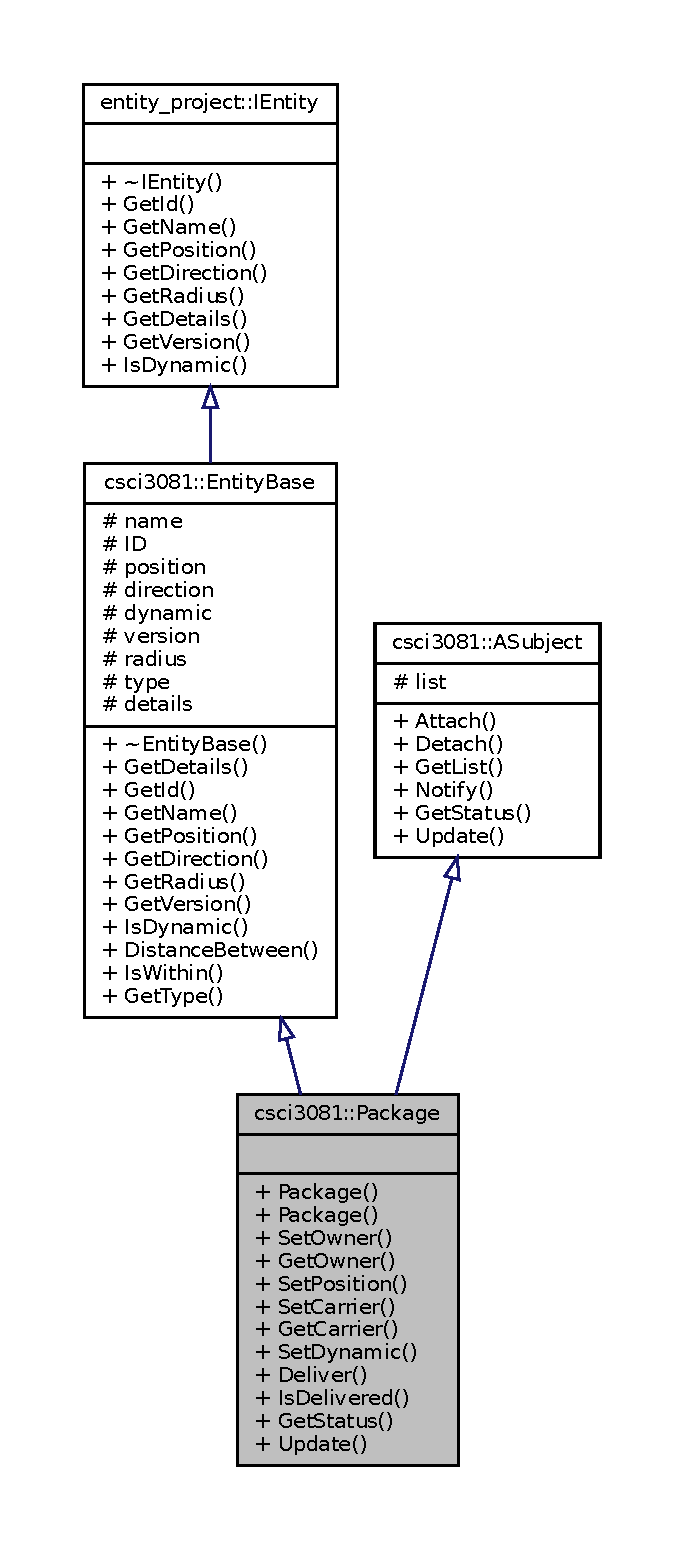
\includegraphics[height=550pt]{classcsci3081_1_1Package__inherit__graph}
\end{center}
\end{figure}
\subsection*{Public Member Functions}
\begin{DoxyCompactItemize}
\item 
\hyperlink{classcsci3081_1_1Package_abf7f7782bd24ceeae85f4ec6e16a8021}{Package} (const picojson\+::object \&detail)
\item 
\hyperlink{classcsci3081_1_1Package_a9a5517a9f494de1dda493c0613918e00}{Package} (\hyperlink{classcsci3081_1_1Package}{Package} \&package)
\begin{DoxyCompactList}\small\item\em Copy Constructor. This creates a new instance of \hyperlink{classcsci3081_1_1Package}{Package} that has the same content as the \hyperlink{classcsci3081_1_1Package}{Package} argument. \end{DoxyCompactList}\item 
void \hyperlink{classcsci3081_1_1Package_afc93b118e87b8dc43388a0e8f485f830}{Set\+Owner} (\hyperlink{classcsci3081_1_1Customer}{Customer} $\ast$)
\begin{DoxyCompactList}\small\item\em This links a customer object to the package object if the package has not already had a customer. \end{DoxyCompactList}\item 
\mbox{\Hypertarget{classcsci3081_1_1Package_a0d58f83494c174f43a0b94dfbaaebfc7}\label{classcsci3081_1_1Package_a0d58f83494c174f43a0b94dfbaaebfc7}} 
\hyperlink{classcsci3081_1_1Customer}{Customer} $\ast$ \hyperlink{classcsci3081_1_1Package_a0d58f83494c174f43a0b94dfbaaebfc7}{Get\+Owner} ()
\begin{DoxyCompactList}\small\item\em This returns a customer object of the package object if there is one, return N\+U\+LL otherwise. \end{DoxyCompactList}\item 
void \hyperlink{classcsci3081_1_1Package_afc467e1989fa6d08182e22006afcc9cd}{Set\+Position} (std\+::vector$<$ float $>$ agr)
\begin{DoxyCompactList}\small\item\em This function uses to set the new position of the package. However, package only moves in simulation if its dynamic attribute is set to true. \end{DoxyCompactList}\item 
void \hyperlink{classcsci3081_1_1Package_abf6700f1011412936069e7cff9ea86c9}{Set\+Carrier} (\hyperlink{classentity__project_1_1IEntity}{I\+Entity} $\ast$)
\begin{DoxyCompactList}\small\item\em This links a carrier Entity object (drone, truck, robot, etc) to the package object if the package has not already had a one. \end{DoxyCompactList}\item 
\mbox{\Hypertarget{classcsci3081_1_1Package_acf298d89a9d964a38cc451dd3c57f984}\label{classcsci3081_1_1Package_acf298d89a9d964a38cc451dd3c57f984}} 
\hyperlink{classentity__project_1_1IEntity}{I\+Entity} $\ast$ \hyperlink{classcsci3081_1_1Package_acf298d89a9d964a38cc451dd3c57f984}{Get\+Carrier} ()
\begin{DoxyCompactList}\small\item\em This returns the pointer that points to the carrier carrying the package if there is one; return N\+U\+LL otherwise. \end{DoxyCompactList}\item 
void \hyperlink{classcsci3081_1_1Package_aa481bfe50ca15db8c19eadbeac91b889}{Set\+Dynamic} (bool n)
\begin{DoxyCompactList}\small\item\em This changes the dynamic of the drone. Note that for the drone to move on the simulation, dynamic of the drone must be set to true. \end{DoxyCompactList}\item 
\mbox{\Hypertarget{classcsci3081_1_1Package_a6ee0a24832784064cd3938d3cfddb9d7}\label{classcsci3081_1_1Package_a6ee0a24832784064cd3938d3cfddb9d7}} 
void \hyperlink{classcsci3081_1_1Package_a6ee0a24832784064cd3938d3cfddb9d7}{Deliver} ()
\begin{DoxyCompactList}\small\item\em This sets the deliverd attribute of the package to true, signaling that the package has already been delivered. Change the carrier of the package to N\+U\+LL. Change the position of the package to out of the camera of the simulation to \char`\"{}teleport\char`\"{} out of the scene when delivered. \end{DoxyCompactList}\item 
\mbox{\Hypertarget{classcsci3081_1_1Package_a725716addd162b42a08ccddf9bdfcfa9}\label{classcsci3081_1_1Package_a725716addd162b42a08ccddf9bdfcfa9}} 
bool \hyperlink{classcsci3081_1_1Package_a725716addd162b42a08ccddf9bdfcfa9}{Is\+Delivered} ()
\begin{DoxyCompactList}\small\item\em This returns a T\+R\+UE if the package has been delivered, F\+A\+L\+SE otherwise. \end{DoxyCompactList}\item 
\mbox{\Hypertarget{classcsci3081_1_1Package_aaf2a9604fc4d3dd108e4b4002751be05}\label{classcsci3081_1_1Package_aaf2a9604fc4d3dd108e4b4002751be05}} 
void \hyperlink{classcsci3081_1_1Package_aaf2a9604fc4d3dd108e4b4002751be05}{Get\+Status} ()
\begin{DoxyCompactList}\small\item\em Overwritten Get\+Status from \hyperlink{classcsci3081_1_1ASubject}{A\+Subject}. This function creates the arguments required by Notify function and makes call to Notify function. This function should be called when path is added to the package is schedule to deliver, en route (picked up) or delivered. \end{DoxyCompactList}\item 
\mbox{\Hypertarget{classcsci3081_1_1Package_acd1f198a6e087c08e1cfeed0f44a90be}\label{classcsci3081_1_1Package_acd1f198a6e087c08e1cfeed0f44a90be}} 
void \hyperlink{classcsci3081_1_1Package_acd1f198a6e087c08e1cfeed0f44a90be}{Update} (float dt)
\begin{DoxyCompactList}\small\item\em This is an inherited method from \hyperlink{classcsci3081_1_1EntityBase}{Entity\+Base} to use for \hyperlink{classcsci3081_1_1DeliverySimulation}{Delivery\+Simulation}. This updates the position of the package on the simulation if the position changes and its dynamic is set to true. \end{DoxyCompactList}\end{DoxyCompactItemize}
\subsection*{Additional Inherited Members}


\subsection{Detailed Description}
A representation of a \hyperlink{classcsci3081_1_1Package}{Package}, inherited from \hyperlink{classcsci3081_1_1EntityBase}{Entity\+Base} It stores the \hyperlink{classcsci3081_1_1Package}{Package}\textquotesingle{}s name, ID, version, position, direction, and dynamic mode. 

\subsection{Constructor \& Destructor Documentation}
\mbox{\Hypertarget{classcsci3081_1_1Package_abf7f7782bd24ceeae85f4ec6e16a8021}\label{classcsci3081_1_1Package_abf7f7782bd24ceeae85f4ec6e16a8021}} 
\index{csci3081\+::\+Package@{csci3081\+::\+Package}!Package@{Package}}
\index{Package@{Package}!csci3081\+::\+Package@{csci3081\+::\+Package}}
\subsubsection{\texorpdfstring{Package()}{Package()}\hspace{0.1cm}{\footnotesize\ttfamily [1/2]}}
{\footnotesize\ttfamily csci3081\+::\+Package\+::\+Package (\begin{DoxyParamCaption}\item[{const picojson\+::object \&}]{detail }\end{DoxyParamCaption})}

Constructor, creates a \hyperlink{classcsci3081_1_1Package}{Package} object param\mbox{[}in\mbox{]} detail a picojson\+::object object that has the detail of the package including name, position, direction, and radius \mbox{\Hypertarget{classcsci3081_1_1Package_a9a5517a9f494de1dda493c0613918e00}\label{classcsci3081_1_1Package_a9a5517a9f494de1dda493c0613918e00}} 
\index{csci3081\+::\+Package@{csci3081\+::\+Package}!Package@{Package}}
\index{Package@{Package}!csci3081\+::\+Package@{csci3081\+::\+Package}}
\subsubsection{\texorpdfstring{Package()}{Package()}\hspace{0.1cm}{\footnotesize\ttfamily [2/2]}}
{\footnotesize\ttfamily csci3081\+::\+Package\+::\+Package (\begin{DoxyParamCaption}\item[{\hyperlink{classcsci3081_1_1Package}{Package} \&}]{package }\end{DoxyParamCaption})}



Copy Constructor. This creates a new instance of \hyperlink{classcsci3081_1_1Package}{Package} that has the same content as the \hyperlink{classcsci3081_1_1Package}{Package} argument. 


\begin{DoxyParams}[1]{Parameters}
\mbox{\tt in}  & {\em package} & \hyperlink{classcsci3081_1_1Package}{Package} instance that wants to be copied \\
\hline
\end{DoxyParams}


\subsection{Member Function Documentation}
\mbox{\Hypertarget{classcsci3081_1_1Package_abf6700f1011412936069e7cff9ea86c9}\label{classcsci3081_1_1Package_abf6700f1011412936069e7cff9ea86c9}} 
\index{csci3081\+::\+Package@{csci3081\+::\+Package}!Set\+Carrier@{Set\+Carrier}}
\index{Set\+Carrier@{Set\+Carrier}!csci3081\+::\+Package@{csci3081\+::\+Package}}
\subsubsection{\texorpdfstring{Set\+Carrier()}{SetCarrier()}}
{\footnotesize\ttfamily void csci3081\+::\+Package\+::\+Set\+Carrier (\begin{DoxyParamCaption}\item[{\hyperlink{classentity__project_1_1IEntity}{I\+Entity} $\ast$}]{ve }\end{DoxyParamCaption})}



This links a carrier Entity object (drone, truck, robot, etc) to the package object if the package has not already had a one. 


\begin{DoxyParams}[1]{Parameters}
\mbox{\tt in}  & {\em o} & a I\+Entity pointer \\
\hline
\end{DoxyParams}
\mbox{\Hypertarget{classcsci3081_1_1Package_aa481bfe50ca15db8c19eadbeac91b889}\label{classcsci3081_1_1Package_aa481bfe50ca15db8c19eadbeac91b889}} 
\index{csci3081\+::\+Package@{csci3081\+::\+Package}!Set\+Dynamic@{Set\+Dynamic}}
\index{Set\+Dynamic@{Set\+Dynamic}!csci3081\+::\+Package@{csci3081\+::\+Package}}
\subsubsection{\texorpdfstring{Set\+Dynamic()}{SetDynamic()}}
{\footnotesize\ttfamily void csci3081\+::\+Package\+::\+Set\+Dynamic (\begin{DoxyParamCaption}\item[{bool}]{n }\end{DoxyParamCaption})}



This changes the dynamic of the drone. Note that for the drone to move on the simulation, dynamic of the drone must be set to true. 


\begin{DoxyParams}[1]{Parameters}
\mbox{\tt in}  & {\em n} & True if the drone is actively moving in the simulation False otherwise \\
\hline
\end{DoxyParams}
\mbox{\Hypertarget{classcsci3081_1_1Package_afc93b118e87b8dc43388a0e8f485f830}\label{classcsci3081_1_1Package_afc93b118e87b8dc43388a0e8f485f830}} 
\index{csci3081\+::\+Package@{csci3081\+::\+Package}!Set\+Owner@{Set\+Owner}}
\index{Set\+Owner@{Set\+Owner}!csci3081\+::\+Package@{csci3081\+::\+Package}}
\subsubsection{\texorpdfstring{Set\+Owner()}{SetOwner()}}
{\footnotesize\ttfamily void csci3081\+::\+Package\+::\+Set\+Owner (\begin{DoxyParamCaption}\item[{\hyperlink{classcsci3081_1_1Customer}{Customer} $\ast$}]{o }\end{DoxyParamCaption})}



This links a customer object to the package object if the package has not already had a customer. 


\begin{DoxyParams}[1]{Parameters}
\mbox{\tt in}  & {\em o} & a \hyperlink{classcsci3081_1_1Customer}{Customer} pointer \\
\hline
\end{DoxyParams}
\mbox{\Hypertarget{classcsci3081_1_1Package_afc467e1989fa6d08182e22006afcc9cd}\label{classcsci3081_1_1Package_afc467e1989fa6d08182e22006afcc9cd}} 
\index{csci3081\+::\+Package@{csci3081\+::\+Package}!Set\+Position@{Set\+Position}}
\index{Set\+Position@{Set\+Position}!csci3081\+::\+Package@{csci3081\+::\+Package}}
\subsubsection{\texorpdfstring{Set\+Position()}{SetPosition()}}
{\footnotesize\ttfamily void csci3081\+::\+Package\+::\+Set\+Position (\begin{DoxyParamCaption}\item[{std\+::vector$<$ float $>$}]{agr }\end{DoxyParamCaption})}



This function uses to set the new position of the package. However, package only moves in simulation if its dynamic attribute is set to true. 


\begin{DoxyParams}{Parameters}
{\em agr} & a std\+::vector$<$float$>$ that has the new position of the package \\
\hline
\end{DoxyParams}


The documentation for this class was generated from the following files\+:\begin{DoxyCompactItemize}
\item 
/home/user/repo/project/include/package.\+h\item 
/home/user/repo/project/src/package.\+cc\end{DoxyCompactItemize}

\hypertarget{classcsci3081_1_1PackageFactory}{}\section{csci3081\+:\+:Package\+Factory Class Reference}
\label{classcsci3081_1_1PackageFactory}\index{csci3081\+::\+Package\+Factory@{csci3081\+::\+Package\+Factory}}


This is the \hyperlink{classcsci3081_1_1PackageFactory}{Package\+Factory}, responsible for making \hyperlink{classcsci3081_1_1Drone}{Drone} object.  




{\ttfamily \#include $<$package\+\_\+factory.\+h$>$}



Inheritance diagram for csci3081\+:\+:Package\+Factory\+:
\nopagebreak
\begin{figure}[H]
\begin{center}
\leavevmode
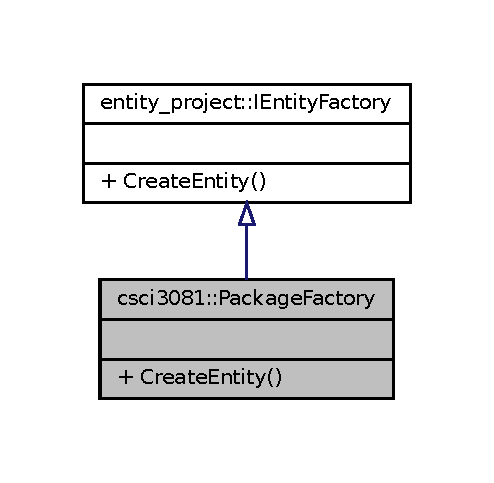
\includegraphics[width=237pt]{classcsci3081_1_1PackageFactory__inherit__graph}
\end{center}
\end{figure}
\subsection*{Public Member Functions}
\begin{DoxyCompactItemize}
\item 
\hyperlink{classentity__project_1_1IEntity}{I\+Entity} $\ast$ \hyperlink{classcsci3081_1_1PackageFactory_ac95467baa4ab68a96ce114548e0b5089}{Create\+Entity} (const picojson\+::object \&val)
\begin{DoxyCompactList}\small\item\em This is an inheritance function from I\+Entity\+Factory to create an approxiate Entity object based on the argument pass in Given the picojson\+::object val, this should create an entity. Based on the type of entity, there may be different fields. You can see the vals that will be passed in the project/web/scenes directory. Some of the fields are for our backend system and you don\textquotesingle{}t need to worry about them. (for instance, mesh, rotation, offset, etc.) \end{DoxyCompactList}\end{DoxyCompactItemize}


\subsection{Detailed Description}
This is the \hyperlink{classcsci3081_1_1PackageFactory}{Package\+Factory}, responsible for making \hyperlink{classcsci3081_1_1Drone}{Drone} object. 

\subsection{Member Function Documentation}
\mbox{\Hypertarget{classcsci3081_1_1PackageFactory_ac95467baa4ab68a96ce114548e0b5089}\label{classcsci3081_1_1PackageFactory_ac95467baa4ab68a96ce114548e0b5089}} 
\index{csci3081\+::\+Package\+Factory@{csci3081\+::\+Package\+Factory}!Create\+Entity@{Create\+Entity}}
\index{Create\+Entity@{Create\+Entity}!csci3081\+::\+Package\+Factory@{csci3081\+::\+Package\+Factory}}
\subsubsection{\texorpdfstring{Create\+Entity()}{CreateEntity()}}
{\footnotesize\ttfamily \hyperlink{classentity__project_1_1IEntity}{I\+Entity} $\ast$ csci3081\+::\+Package\+Factory\+::\+Create\+Entity (\begin{DoxyParamCaption}\item[{const picojson\+::object \&}]{val }\end{DoxyParamCaption})\hspace{0.3cm}{\ttfamily [virtual]}}



This is an inheritance function from I\+Entity\+Factory to create an approxiate Entity object based on the argument pass in Given the picojson\+::object val, this should create an entity. Based on the type of entity, there may be different fields. You can see the vals that will be passed in the project/web/scenes directory. Some of the fields are for our backend system and you don\textquotesingle{}t need to worry about them. (for instance, mesh, rotation, offset, etc.) 

Some fields in val that you will need to create the entity correctly\+:

type\+: string (could be \char`\"{}drone/customer/package\char`\"{})

name\+: string

position\+: array (contains \mbox{[}x\+\_\+position, y\+\_\+position, z\+\_\+position\mbox{]})

direction\+: array (contains \mbox{[}x, y, z\mbox{]})


\begin{DoxyParams}[1]{Parameters}
\mbox{\tt in}  & {\em val} & the picojson\+::object that constains all of the necessary information above in a json format \\
\hline
\end{DoxyParams}
\begin{DoxyReturn}{Returns}
I\+Entity pointer if the object has type \char`\"{}package\char`\"{}; N\+U\+LL otherwise 
\end{DoxyReturn}


Implements \hyperlink{classentity__project_1_1IEntityFactory_ac4e8eaf4294958fef0b98bd3684704bb}{entity\+\_\+project\+::\+I\+Entity\+Factory}.



The documentation for this class was generated from the following files\+:\begin{DoxyCompactItemize}
\item 
/home/user/repo/project/include/package\+\_\+factory.\+h\item 
/home/user/repo/project/src/package\+\_\+factory.\+cc\end{DoxyCompactItemize}

\hypertarget{classcsci3081_1_1ParabolicRoute}{}\section{csci3081\+:\+:Parabolic\+Route Class Reference}
\label{classcsci3081_1_1ParabolicRoute}\index{csci3081\+::\+Parabolic\+Route@{csci3081\+::\+Parabolic\+Route}}


This is the Parabolic Route class where we can use the strategy pattern to implement a parabolic route.  




{\ttfamily \#include $<$parabolic\+\_\+route.\+h$>$}



Inheritance diagram for csci3081\+:\+:Parabolic\+Route\+:
\nopagebreak
\begin{figure}[H]
\begin{center}
\leavevmode
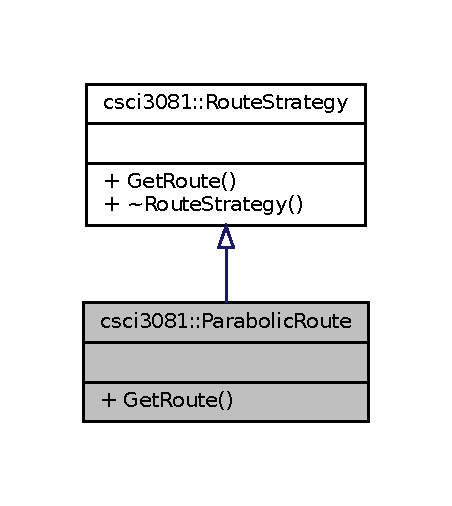
\includegraphics[width=217pt]{classcsci3081_1_1ParabolicRoute__inherit__graph}
\end{center}
\end{figure}
\subsection*{Public Member Functions}
\begin{DoxyCompactItemize}
\item 
std\+::vector$<$ std\+::vector$<$ float $>$ $>$ \hyperlink{classcsci3081_1_1ParabolicRoute_adbafff4df041bd49c060578216cb77fc}{Get\+Route} (const \hyperlink{classentity__project_1_1IGraph}{I\+Graph} $\ast$graph, std\+::vector$<$ float $>$ location, std\+::vector$<$ float $>$ dest)
\begin{DoxyCompactList}\small\item\em This function allows the moving item to get the desired route. In this class, the function will return a route that follows the parabolic path. However a pure parabolic path will make the drone clips the building at the end. What we did is raise the drone to a certain height first,then do parabolic in the air and descend veritcally. \end{DoxyCompactList}\end{DoxyCompactItemize}


\subsection{Detailed Description}
This is the Parabolic Route class where we can use the strategy pattern to implement a parabolic route. 

\subsection{Member Function Documentation}
\mbox{\Hypertarget{classcsci3081_1_1ParabolicRoute_adbafff4df041bd49c060578216cb77fc}\label{classcsci3081_1_1ParabolicRoute_adbafff4df041bd49c060578216cb77fc}} 
\index{csci3081\+::\+Parabolic\+Route@{csci3081\+::\+Parabolic\+Route}!Get\+Route@{Get\+Route}}
\index{Get\+Route@{Get\+Route}!csci3081\+::\+Parabolic\+Route@{csci3081\+::\+Parabolic\+Route}}
\subsubsection{\texorpdfstring{Get\+Route()}{GetRoute()}}
{\footnotesize\ttfamily std\+::vector$<$ std\+::vector$<$ float $>$ $>$ csci3081\+::\+Parabolic\+Route\+::\+Get\+Route (\begin{DoxyParamCaption}\item[{const \hyperlink{classentity__project_1_1IGraph}{I\+Graph} $\ast$}]{graph,  }\item[{std\+::vector$<$ float $>$}]{location,  }\item[{std\+::vector$<$ float $>$}]{dest }\end{DoxyParamCaption})\hspace{0.3cm}{\ttfamily [virtual]}}



This function allows the moving item to get the desired route. In this class, the function will return a route that follows the parabolic path. However a pure parabolic path will make the drone clips the building at the end. What we did is raise the drone to a certain height first,then do parabolic in the air and descend veritcally. 


\begin{DoxyParams}{Parameters}
{\em const} & I\+Graph$\ast$ graph \\
\hline
{\em std\+::vector$<$float$>$} & location \\
\hline
{\em std\+::vector$<$float$>$} & dest \\
\hline
\end{DoxyParams}
\begin{DoxyReturn}{Returns}
std\+::vector $<$std\+::vector$<$float$>$$>$ 
\end{DoxyReturn}


Implements \hyperlink{classcsci3081_1_1RouteStrategy_a4bf67b185a4446324ebc13c1cda40cfe}{csci3081\+::\+Route\+Strategy}.



The documentation for this class was generated from the following files\+:\begin{DoxyCompactItemize}
\item 
/home/user/repo/project/include/parabolic\+\_\+route.\+h\item 
/home/user/repo/project/src/parabolic\+\_\+route.\+cc\end{DoxyCompactItemize}

\hypertarget{classcsci3081_1_1RechargeDrone}{}\section{csci3081\+:\+:Recharge\+Drone Class Reference}
\label{classcsci3081_1_1RechargeDrone}\index{csci3081\+::\+Recharge\+Drone@{csci3081\+::\+Recharge\+Drone}}


A representation of a drone It stores the drone\textquotesingle{}s name, ID, version, position, direction, speed, and dynamic mode.  




{\ttfamily \#include $<$recharge\+\_\+drone.\+h$>$}



Inheritance diagram for csci3081\+:\+:Recharge\+Drone\+:
\nopagebreak
\begin{figure}[H]
\begin{center}
\leavevmode
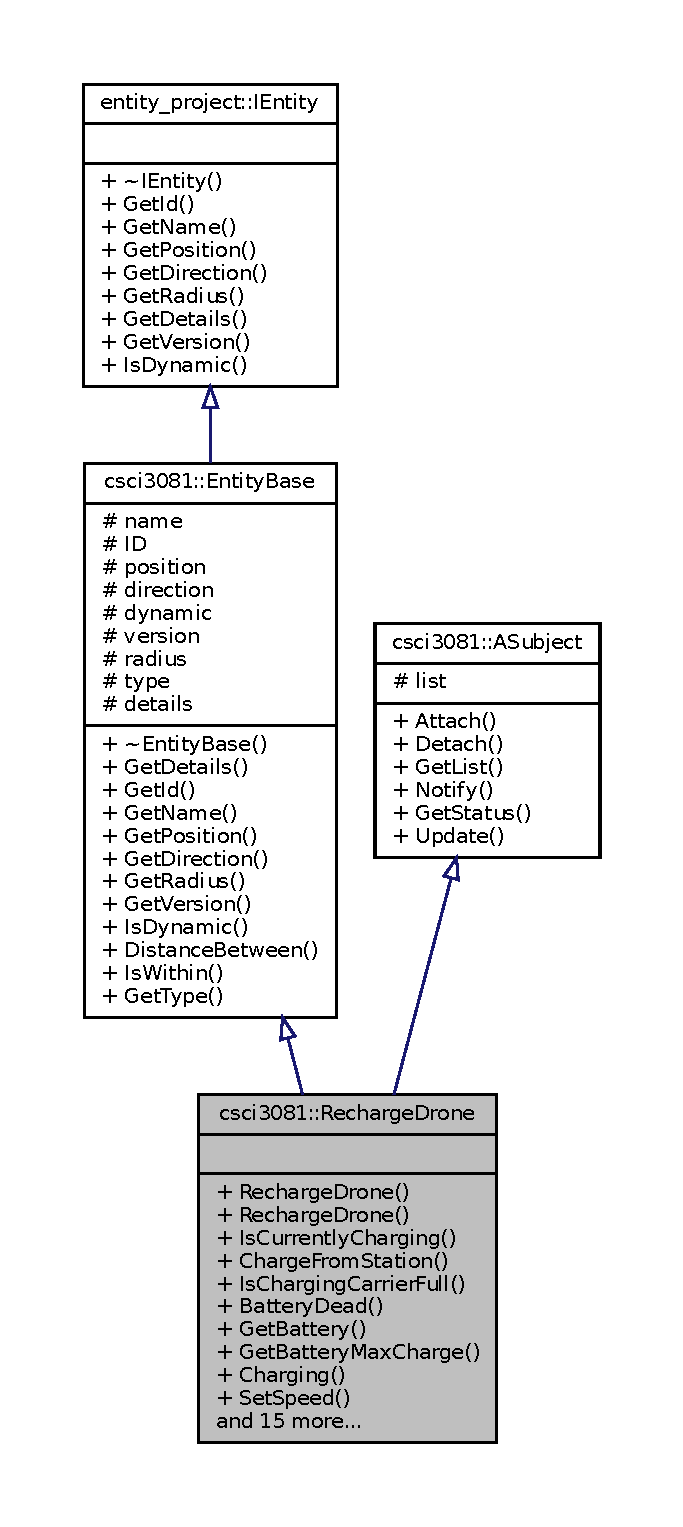
\includegraphics[height=550pt]{classcsci3081_1_1RechargeDrone__inherit__graph}
\end{center}
\end{figure}
\subsection*{Public Member Functions}
\begin{DoxyCompactItemize}
\item 
\hyperlink{classcsci3081_1_1RechargeDrone_a04313869575a751f7f763cf72c2e6410}{Recharge\+Drone} (const picojson\+::object \&val)
\item 
\hyperlink{classcsci3081_1_1RechargeDrone_aa7f639598af768a3c92c082f5d4e74fd}{Recharge\+Drone} (\hyperlink{classcsci3081_1_1RechargeDrone}{Recharge\+Drone} \&)
\begin{DoxyCompactList}\small\item\em Copy Constructor. This creates a new instance of recharing drone that has the same content as the \hyperlink{classcsci3081_1_1Package}{Package} argument. \end{DoxyCompactList}\item 
bool \hyperlink{classcsci3081_1_1RechargeDrone_a21f38d9534ed51a82006df0a4d7ab78e}{Is\+Currently\+Charging} ()
\begin{DoxyCompactList}\small\item\em This function will charge the recharging drone at the station when there is no Dead\+Carrier. \end{DoxyCompactList}\item 
void \hyperlink{classcsci3081_1_1RechargeDrone_aae4cc9921818edce62664130e29cc205}{Charge\+From\+Station} (float dt)
\begin{DoxyCompactList}\small\item\em This function will charge the recharging drone at the station when there is no Dead\+Carrier. \end{DoxyCompactList}\item 
bool \hyperlink{classcsci3081_1_1RechargeDrone_af6c18a005a235b569b10225f9f0b3d78}{Is\+Charging\+Carrier\+Full} (float dt)
\begin{DoxyCompactList}\small\item\em This function will charge the Dead\+Carrier if the Dead\+Carrier is not charged to full. After the Dead\+Carrier get charged to full it will set the Dead\+Carrier Charging Status to false so the simulation will know the Dead\+Carrier is ready to be schduled. \end{DoxyCompactList}\item 
bool \hyperlink{classcsci3081_1_1RechargeDrone_a17d45a9ee48936ddbe019e8ab677f7cf}{Battery\+Dead} ()
\begin{DoxyCompactList}\small\item\em This checks if the recharging drone is out of battery. \end{DoxyCompactList}\item 
\mbox{\Hypertarget{classcsci3081_1_1RechargeDrone_a77787f8e9b4ae3b3575e6c68ba3e8ca3}\label{classcsci3081_1_1RechargeDrone_a77787f8e9b4ae3b3575e6c68ba3e8ca3}} 
float \hyperlink{classcsci3081_1_1RechargeDrone_a77787f8e9b4ae3b3575e6c68ba3e8ca3}{Get\+Battery} ()
\begin{DoxyCompactList}\small\item\em This returns the time in secs left in the carrier\textquotesingle{}s battery. \end{DoxyCompactList}\item 
\mbox{\Hypertarget{classcsci3081_1_1RechargeDrone_a52a715c52891edfcc9a31b06c30d6198}\label{classcsci3081_1_1RechargeDrone_a52a715c52891edfcc9a31b06c30d6198}} 
float \hyperlink{classcsci3081_1_1RechargeDrone_a52a715c52891edfcc9a31b06c30d6198}{Get\+Battery\+Max\+Charge} ()
\begin{DoxyCompactList}\small\item\em This returns the max charge of the recharge drone\textquotesingle{}s battery. \end{DoxyCompactList}\item 
bool \hyperlink{classcsci3081_1_1RechargeDrone_a54f93680add2c289a2b354e1331ad81f}{Charging} (float)
\begin{DoxyCompactList}\small\item\em This function is used to charge the battery of the carrier for a certain amount of time in seconds. \end{DoxyCompactList}\item 
void \hyperlink{classcsci3081_1_1RechargeDrone_a4cfa100bfeabb0b9c893c74a6aeffc23}{Set\+Speed} (float)
\begin{DoxyCompactList}\small\item\em This sets the speed of the carrier. Change the speed of the carrier if the argument is a non-\/negative float number. \end{DoxyCompactList}\item 
\mbox{\Hypertarget{classcsci3081_1_1RechargeDrone_aded486fd6cf88c9f773953daf3d492a4}\label{classcsci3081_1_1RechargeDrone_aded486fd6cf88c9f773953daf3d492a4}} 
float \hyperlink{classcsci3081_1_1RechargeDrone_aded486fd6cf88c9f773953daf3d492a4}{Get\+Speed} ()
\begin{DoxyCompactList}\small\item\em return the current speed of the carrier \end{DoxyCompactList}\item 
void \hyperlink{classcsci3081_1_1RechargeDrone_a226ad5a957052707e19d986a94a53c2d}{Set\+Position} (std\+::vector$<$ float $>$ v)
\begin{DoxyCompactList}\small\item\em This function uses to set the new position of the carrier. However, carrier only moves in simulation if its dynamic attribute is set to true. \end{DoxyCompactList}\item 
void \hyperlink{classcsci3081_1_1RechargeDrone_a2c3e7c4f5c4ca78feef664fca810d0ea}{Set\+Dynamic} (bool dynamic\+\_\+)
\begin{DoxyCompactList}\small\item\em This changes the dynamic of the recharge drone. Note that for the recharge drone to move on the simulation, dynamic of the recharge drone must be set to true. \end{DoxyCompactList}\item 
void \hyperlink{classcsci3081_1_1RechargeDrone_a06c5c7bde0b661c5920ad9dc0e8e5420}{Set\+Route} (std\+::vector$<$ vector$<$ float $>$$>$)
\begin{DoxyCompactList}\small\item\em This function adds a full route to route attribute of the carrier This is useful when use for the Get\+Path() function from I\+Graph class. \end{DoxyCompactList}\item 
\mbox{\Hypertarget{classcsci3081_1_1RechargeDrone_abf8979f7773a6a280eefedf344992356}\label{classcsci3081_1_1RechargeDrone_abf8979f7773a6a280eefedf344992356}} 
std\+::vector$<$ float $>$ \hyperlink{classcsci3081_1_1RechargeDrone_abf8979f7773a6a280eefedf344992356}{Next\+Position} ()
\begin{DoxyCompactList}\small\item\em This function returns the next position in std\+::vector$<$float$>$ in the queue that the carrier needs to move to. \end{DoxyCompactList}\item 
\mbox{\Hypertarget{classcsci3081_1_1RechargeDrone_af4901b3bd3755500a4841a1318022359}\label{classcsci3081_1_1RechargeDrone_af4901b3bd3755500a4841a1318022359}} 
void \hyperlink{classcsci3081_1_1RechargeDrone_af4901b3bd3755500a4841a1318022359}{Pop\+Position} ()
\begin{DoxyCompactList}\small\item\em This function pops the first element/position in the position queue of the carrier. \end{DoxyCompactList}\item 
\mbox{\Hypertarget{classcsci3081_1_1RechargeDrone_ac4b45136e2969ac25941d46a8ccdb83a}\label{classcsci3081_1_1RechargeDrone_ac4b45136e2969ac25941d46a8ccdb83a}} 
void \hyperlink{classcsci3081_1_1RechargeDrone_ac4b45136e2969ac25941d46a8ccdb83a}{Update} (float dt)
\begin{DoxyCompactList}\small\item\em This is an inherited method from \hyperlink{classcsci3081_1_1EntityBase}{Entity\+Base} to use for \hyperlink{classcsci3081_1_1DeliverySimulation}{Delivery\+Simulation}. This updates the position of the carrier on the simulation if the position changes and its dynamic is set to true. In addition, this function also checks if the carrier is in within distance with the package to pick it up, or within distance with the customer to drop off the package. \end{DoxyCompactList}\item 
void \hyperlink{classcsci3081_1_1RechargeDrone_aa245b79215b39c86c1f9fde874bdf264}{Get\+Status} ()
\begin{DoxyCompactList}\small\item\em Overwritten Get\+Status from \hyperlink{classcsci3081_1_1ASubject}{A\+Subject}. This function creates the arguments required by Notify function and makes call to Notify function. This function should be called when path is added to the carrier and when the carrier becomes idle. \end{DoxyCompactList}\item 
void \hyperlink{classcsci3081_1_1RechargeDrone_ab1acfe860678cd982e0d65be34d4e1d7}{Set\+Dead\+Carrier} (\hyperlink{classcsci3081_1_1Carrier}{Carrier} $\ast$carrier)
\begin{DoxyCompactList}\small\item\em This function set the Dead\+Carrier Pointer to a new carrier. \end{DoxyCompactList}\item 
\hyperlink{classcsci3081_1_1Carrier}{Carrier} $\ast$ \hyperlink{classcsci3081_1_1RechargeDrone_a3e8eae4e2d65ba366f0935354262d48a}{Get\+Dead\+Carrier} ()
\begin{DoxyCompactList}\small\item\em This function set the Dead\+Carrier Pointer to a new carrier. \end{DoxyCompactList}\item 
void \hyperlink{classcsci3081_1_1RechargeDrone_a0bd3d0f578960d5a58842781c8dccd46}{Set\+Position\+Of\+Station} (vector$<$ float $>$ station)
\begin{DoxyCompactList}\small\item\em This function set the position of the station(\+Set\+Position\+Of\+Station) to a new position. \end{DoxyCompactList}\item 
vector$<$ float $>$ \hyperlink{classcsci3081_1_1RechargeDrone_aa8116aa4337b43f649adaf21db0d0b08}{Get\+Position\+Of\+Station} ()
\begin{DoxyCompactList}\small\item\em This function Get the position of the station(\+Set\+Position\+Of\+Station) \end{DoxyCompactList}\item 
bool \hyperlink{classcsci3081_1_1RechargeDrone_af84e518c7cf9b47b47c8c0fe21883272}{Is\+Charging\+A\+Carrier} ()
\begin{DoxyCompactList}\small\item\em This function should check the Dead\+Carrier pointer if its null or not and check if the Dead\+Carrier is getting charged or not. This function should be called in the simulation that to check the status of the recharging\+\_\+drone. If its charing a Dead\+Carrier then does not need to Update the recharging drone. \end{DoxyCompactList}\item 
\hyperlink{classcsci3081_1_1RouteStrategy}{Route\+Strategy} $\ast$ \hyperlink{classcsci3081_1_1RechargeDrone_a5dacec43761a0e06f063c04f56654346}{Get\+Route\+Strategy} ()
\begin{DoxyCompactList}\small\item\em return the Route Strategy that the carrier uses, such as Smart Route, Beeline, or Parabolic Route \end{DoxyCompactList}\item 
bool \hyperlink{classcsci3081_1_1RechargeDrone_acc49b5dd6e59d7bc14be53536648288a}{Battery\+Full} ()
\begin{DoxyCompactList}\small\item\em This function checks the battery Capacity to see if it\textquotesingle{}s full or not. This function should be called in \hyperlink{classcsci3081_1_1RechargeDrone_af6c18a005a235b569b10225f9f0b3d78}{Is\+Charging\+Carrier\+Full()} to check if the Dead\+Drone need to be charged more. \end{DoxyCompactList}\end{DoxyCompactItemize}
\subsection*{Additional Inherited Members}


\subsection{Detailed Description}
A representation of a drone It stores the drone\textquotesingle{}s name, ID, version, position, direction, speed, and dynamic mode. 

\subsection{Constructor \& Destructor Documentation}
\mbox{\Hypertarget{classcsci3081_1_1RechargeDrone_a04313869575a751f7f763cf72c2e6410}\label{classcsci3081_1_1RechargeDrone_a04313869575a751f7f763cf72c2e6410}} 
\index{csci3081\+::\+Recharge\+Drone@{csci3081\+::\+Recharge\+Drone}!Recharge\+Drone@{Recharge\+Drone}}
\index{Recharge\+Drone@{Recharge\+Drone}!csci3081\+::\+Recharge\+Drone@{csci3081\+::\+Recharge\+Drone}}
\subsubsection{\texorpdfstring{Recharge\+Drone()}{RechargeDrone()}\hspace{0.1cm}{\footnotesize\ttfamily [1/2]}}
{\footnotesize\ttfamily csci3081\+::\+Recharge\+Drone\+::\+Recharge\+Drone (\begin{DoxyParamCaption}\item[{const picojson\+::object \&}]{val }\end{DoxyParamCaption})}

Constructor, creates a recharing drone object param\mbox{[}in\mbox{]} val a picojson\+::object object that has the detail of the package including name, position, direction, radius, and speed \mbox{\Hypertarget{classcsci3081_1_1RechargeDrone_aa7f639598af768a3c92c082f5d4e74fd}\label{classcsci3081_1_1RechargeDrone_aa7f639598af768a3c92c082f5d4e74fd}} 
\index{csci3081\+::\+Recharge\+Drone@{csci3081\+::\+Recharge\+Drone}!Recharge\+Drone@{Recharge\+Drone}}
\index{Recharge\+Drone@{Recharge\+Drone}!csci3081\+::\+Recharge\+Drone@{csci3081\+::\+Recharge\+Drone}}
\subsubsection{\texorpdfstring{Recharge\+Drone()}{RechargeDrone()}\hspace{0.1cm}{\footnotesize\ttfamily [2/2]}}
{\footnotesize\ttfamily csci3081\+::\+Recharge\+Drone\+::\+Recharge\+Drone (\begin{DoxyParamCaption}\item[{\hyperlink{classcsci3081_1_1RechargeDrone}{Recharge\+Drone} \&}]{cpy }\end{DoxyParamCaption})}



Copy Constructor. This creates a new instance of recharing drone that has the same content as the \hyperlink{classcsci3081_1_1Package}{Package} argument. 


\begin{DoxyParams}[1]{Parameters}
\mbox{\tt in}  & {\em cpy} & \hyperlink{classcsci3081_1_1Drone}{Drone} instance that wants to be copied \\
\hline
\end{DoxyParams}


\subsection{Member Function Documentation}
\mbox{\Hypertarget{classcsci3081_1_1RechargeDrone_a17d45a9ee48936ddbe019e8ab677f7cf}\label{classcsci3081_1_1RechargeDrone_a17d45a9ee48936ddbe019e8ab677f7cf}} 
\index{csci3081\+::\+Recharge\+Drone@{csci3081\+::\+Recharge\+Drone}!Battery\+Dead@{Battery\+Dead}}
\index{Battery\+Dead@{Battery\+Dead}!csci3081\+::\+Recharge\+Drone@{csci3081\+::\+Recharge\+Drone}}
\subsubsection{\texorpdfstring{Battery\+Dead()}{BatteryDead()}}
{\footnotesize\ttfamily bool csci3081\+::\+Recharge\+Drone\+::\+Battery\+Dead (\begin{DoxyParamCaption}{ }\end{DoxyParamCaption})}



This checks if the recharging drone is out of battery. 

\begin{DoxyReturn}{Returns}
T\+R\+UE if the battery of the carrier is out F\+A\+L\+SE otherwise 
\end{DoxyReturn}
\mbox{\Hypertarget{classcsci3081_1_1RechargeDrone_acc49b5dd6e59d7bc14be53536648288a}\label{classcsci3081_1_1RechargeDrone_acc49b5dd6e59d7bc14be53536648288a}} 
\index{csci3081\+::\+Recharge\+Drone@{csci3081\+::\+Recharge\+Drone}!Battery\+Full@{Battery\+Full}}
\index{Battery\+Full@{Battery\+Full}!csci3081\+::\+Recharge\+Drone@{csci3081\+::\+Recharge\+Drone}}
\subsubsection{\texorpdfstring{Battery\+Full()}{BatteryFull()}}
{\footnotesize\ttfamily bool csci3081\+::\+Recharge\+Drone\+::\+Battery\+Full (\begin{DoxyParamCaption}{ }\end{DoxyParamCaption})}



This function checks the battery Capacity to see if it\textquotesingle{}s full or not. This function should be called in \hyperlink{classcsci3081_1_1RechargeDrone_af6c18a005a235b569b10225f9f0b3d78}{Is\+Charging\+Carrier\+Full()} to check if the Dead\+Drone need to be charged more. 

\begin{DoxyReturn}{Returns}
the boolean value that indicates ss the battery full or not 
\end{DoxyReturn}
\mbox{\Hypertarget{classcsci3081_1_1RechargeDrone_aae4cc9921818edce62664130e29cc205}\label{classcsci3081_1_1RechargeDrone_aae4cc9921818edce62664130e29cc205}} 
\index{csci3081\+::\+Recharge\+Drone@{csci3081\+::\+Recharge\+Drone}!Charge\+From\+Station@{Charge\+From\+Station}}
\index{Charge\+From\+Station@{Charge\+From\+Station}!csci3081\+::\+Recharge\+Drone@{csci3081\+::\+Recharge\+Drone}}
\subsubsection{\texorpdfstring{Charge\+From\+Station()}{ChargeFromStation()}}
{\footnotesize\ttfamily void csci3081\+::\+Recharge\+Drone\+::\+Charge\+From\+Station (\begin{DoxyParamCaption}\item[{float}]{dt }\end{DoxyParamCaption})}



This function will charge the recharging drone at the station when there is no Dead\+Carrier. 


\begin{DoxyParams}[1]{Parameters}
\mbox{\tt in}  & {\em t} & time that charge the recharging drone \\
\hline
\end{DoxyParams}
\mbox{\Hypertarget{classcsci3081_1_1RechargeDrone_a54f93680add2c289a2b354e1331ad81f}\label{classcsci3081_1_1RechargeDrone_a54f93680add2c289a2b354e1331ad81f}} 
\index{csci3081\+::\+Recharge\+Drone@{csci3081\+::\+Recharge\+Drone}!Charging@{Charging}}
\index{Charging@{Charging}!csci3081\+::\+Recharge\+Drone@{csci3081\+::\+Recharge\+Drone}}
\subsubsection{\texorpdfstring{Charging()}{Charging()}}
{\footnotesize\ttfamily bool csci3081\+::\+Recharge\+Drone\+::\+Charging (\begin{DoxyParamCaption}\item[{float}]{sec }\end{DoxyParamCaption})}



This function is used to charge the battery of the carrier for a certain amount of time in seconds. 


\begin{DoxyParams}[1]{Parameters}
\mbox{\tt in}  & {\em sec} & amount of time in secs to charge the battery \\
\hline
\end{DoxyParams}
\begin{DoxyReturn}{Returns}
T\+R\+UE if the battery can be charged F\+A\+L\+SE otherwise 
\end{DoxyReturn}
\mbox{\Hypertarget{classcsci3081_1_1RechargeDrone_a3e8eae4e2d65ba366f0935354262d48a}\label{classcsci3081_1_1RechargeDrone_a3e8eae4e2d65ba366f0935354262d48a}} 
\index{csci3081\+::\+Recharge\+Drone@{csci3081\+::\+Recharge\+Drone}!Get\+Dead\+Carrier@{Get\+Dead\+Carrier}}
\index{Get\+Dead\+Carrier@{Get\+Dead\+Carrier}!csci3081\+::\+Recharge\+Drone@{csci3081\+::\+Recharge\+Drone}}
\subsubsection{\texorpdfstring{Get\+Dead\+Carrier()}{GetDeadCarrier()}}
{\footnotesize\ttfamily \hyperlink{classcsci3081_1_1Carrier}{Carrier} $\ast$ csci3081\+::\+Recharge\+Drone\+::\+Get\+Dead\+Carrier (\begin{DoxyParamCaption}{ }\end{DoxyParamCaption})}



This function set the Dead\+Carrier Pointer to a new carrier. 

\begin{DoxyReturn}{Returns}
return the Dead\+Carrier N\+U\+LL for nothing 
\end{DoxyReturn}
\mbox{\Hypertarget{classcsci3081_1_1RechargeDrone_aa8116aa4337b43f649adaf21db0d0b08}\label{classcsci3081_1_1RechargeDrone_aa8116aa4337b43f649adaf21db0d0b08}} 
\index{csci3081\+::\+Recharge\+Drone@{csci3081\+::\+Recharge\+Drone}!Get\+Position\+Of\+Station@{Get\+Position\+Of\+Station}}
\index{Get\+Position\+Of\+Station@{Get\+Position\+Of\+Station}!csci3081\+::\+Recharge\+Drone@{csci3081\+::\+Recharge\+Drone}}
\subsubsection{\texorpdfstring{Get\+Position\+Of\+Station()}{GetPositionOfStation()}}
{\footnotesize\ttfamily vector$<$ float $>$ csci3081\+::\+Recharge\+Drone\+::\+Get\+Position\+Of\+Station (\begin{DoxyParamCaption}{ }\end{DoxyParamCaption})}



This function Get the position of the station(\+Set\+Position\+Of\+Station) 

\begin{DoxyReturn}{Returns}
return the Set\+Position\+Of\+Station(\+N\+U\+L\+L for nothing) 
\end{DoxyReturn}
\mbox{\Hypertarget{classcsci3081_1_1RechargeDrone_a5dacec43761a0e06f063c04f56654346}\label{classcsci3081_1_1RechargeDrone_a5dacec43761a0e06f063c04f56654346}} 
\index{csci3081\+::\+Recharge\+Drone@{csci3081\+::\+Recharge\+Drone}!Get\+Route\+Strategy@{Get\+Route\+Strategy}}
\index{Get\+Route\+Strategy@{Get\+Route\+Strategy}!csci3081\+::\+Recharge\+Drone@{csci3081\+::\+Recharge\+Drone}}
\subsubsection{\texorpdfstring{Get\+Route\+Strategy()}{GetRouteStrategy()}}
{\footnotesize\ttfamily \hyperlink{classcsci3081_1_1RouteStrategy}{Route\+Strategy} $\ast$ csci3081\+::\+Recharge\+Drone\+::\+Get\+Route\+Strategy (\begin{DoxyParamCaption}{ }\end{DoxyParamCaption})}



return the Route Strategy that the carrier uses, such as Smart Route, Beeline, or Parabolic Route 

\begin{DoxyReturn}{Returns}
\hyperlink{classcsci3081_1_1RouteStrategy}{Route\+Strategy} pointer 
\end{DoxyReturn}
\mbox{\Hypertarget{classcsci3081_1_1RechargeDrone_aa245b79215b39c86c1f9fde874bdf264}\label{classcsci3081_1_1RechargeDrone_aa245b79215b39c86c1f9fde874bdf264}} 
\index{csci3081\+::\+Recharge\+Drone@{csci3081\+::\+Recharge\+Drone}!Get\+Status@{Get\+Status}}
\index{Get\+Status@{Get\+Status}!csci3081\+::\+Recharge\+Drone@{csci3081\+::\+Recharge\+Drone}}
\subsubsection{\texorpdfstring{Get\+Status()}{GetStatus()}}
{\footnotesize\ttfamily void csci3081\+::\+Recharge\+Drone\+::\+Get\+Status (\begin{DoxyParamCaption}{ }\end{DoxyParamCaption})\hspace{0.3cm}{\ttfamily [virtual]}}



Overwritten Get\+Status from \hyperlink{classcsci3081_1_1ASubject}{A\+Subject}. This function creates the arguments required by Notify function and makes call to Notify function. This function should be called when path is added to the carrier and when the carrier becomes idle. 


\begin{DoxyParams}{Parameters}
{\em picojson\+::value\&} & event \\
\hline
{\em const} & \hyperlink{classentity__project_1_1IEntity}{entity\+\_\+project\+::\+I\+Entity}\& entity \\
\hline
\end{DoxyParams}


Implements \hyperlink{classcsci3081_1_1ASubject_a206a9ddb559da279011e2f9ea29663dc}{csci3081\+::\+A\+Subject}.

\mbox{\Hypertarget{classcsci3081_1_1RechargeDrone_af84e518c7cf9b47b47c8c0fe21883272}\label{classcsci3081_1_1RechargeDrone_af84e518c7cf9b47b47c8c0fe21883272}} 
\index{csci3081\+::\+Recharge\+Drone@{csci3081\+::\+Recharge\+Drone}!Is\+Charging\+A\+Carrier@{Is\+Charging\+A\+Carrier}}
\index{Is\+Charging\+A\+Carrier@{Is\+Charging\+A\+Carrier}!csci3081\+::\+Recharge\+Drone@{csci3081\+::\+Recharge\+Drone}}
\subsubsection{\texorpdfstring{Is\+Charging\+A\+Carrier()}{IsChargingACarrier()}}
{\footnotesize\ttfamily bool csci3081\+::\+Recharge\+Drone\+::\+Is\+Charging\+A\+Carrier (\begin{DoxyParamCaption}{ }\end{DoxyParamCaption})}



This function should check the Dead\+Carrier pointer if its null or not and check if the Dead\+Carrier is getting charged or not. This function should be called in the simulation that to check the status of the recharging\+\_\+drone. If its charing a Dead\+Carrier then does not need to Update the recharging drone. 

\begin{DoxyReturn}{Returns}
the boolean value that indicates reacharging drone is charging a Dead\+Carrier or not. 
\end{DoxyReturn}
\mbox{\Hypertarget{classcsci3081_1_1RechargeDrone_af6c18a005a235b569b10225f9f0b3d78}\label{classcsci3081_1_1RechargeDrone_af6c18a005a235b569b10225f9f0b3d78}} 
\index{csci3081\+::\+Recharge\+Drone@{csci3081\+::\+Recharge\+Drone}!Is\+Charging\+Carrier\+Full@{Is\+Charging\+Carrier\+Full}}
\index{Is\+Charging\+Carrier\+Full@{Is\+Charging\+Carrier\+Full}!csci3081\+::\+Recharge\+Drone@{csci3081\+::\+Recharge\+Drone}}
\subsubsection{\texorpdfstring{Is\+Charging\+Carrier\+Full()}{IsChargingCarrierFull()}}
{\footnotesize\ttfamily bool csci3081\+::\+Recharge\+Drone\+::\+Is\+Charging\+Carrier\+Full (\begin{DoxyParamCaption}\item[{float}]{dt }\end{DoxyParamCaption})}



This function will charge the Dead\+Carrier if the Dead\+Carrier is not charged to full. After the Dead\+Carrier get charged to full it will set the Dead\+Carrier Charging Status to false so the simulation will know the Dead\+Carrier is ready to be schduled. 


\begin{DoxyParams}[1]{Parameters}
\mbox{\tt in}  & {\em t} & time that charge the recharging drone \\
\hline
\end{DoxyParams}
\begin{DoxyReturn}{Returns}
this function will return true when the Dead\+Carrier get charged to full 
\end{DoxyReturn}
\mbox{\Hypertarget{classcsci3081_1_1RechargeDrone_a21f38d9534ed51a82006df0a4d7ab78e}\label{classcsci3081_1_1RechargeDrone_a21f38d9534ed51a82006df0a4d7ab78e}} 
\index{csci3081\+::\+Recharge\+Drone@{csci3081\+::\+Recharge\+Drone}!Is\+Currently\+Charging@{Is\+Currently\+Charging}}
\index{Is\+Currently\+Charging@{Is\+Currently\+Charging}!csci3081\+::\+Recharge\+Drone@{csci3081\+::\+Recharge\+Drone}}
\subsubsection{\texorpdfstring{Is\+Currently\+Charging()}{IsCurrentlyCharging()}}
{\footnotesize\ttfamily bool csci3081\+::\+Recharge\+Drone\+::\+Is\+Currently\+Charging (\begin{DoxyParamCaption}{ }\end{DoxyParamCaption})}



This function will charge the recharging drone at the station when there is no Dead\+Carrier. 


\begin{DoxyParams}[1]{Parameters}
\mbox{\tt in}  & {\em t} & time that charge the recharging drone \\
\hline
\end{DoxyParams}
\mbox{\Hypertarget{classcsci3081_1_1RechargeDrone_ab1acfe860678cd982e0d65be34d4e1d7}\label{classcsci3081_1_1RechargeDrone_ab1acfe860678cd982e0d65be34d4e1d7}} 
\index{csci3081\+::\+Recharge\+Drone@{csci3081\+::\+Recharge\+Drone}!Set\+Dead\+Carrier@{Set\+Dead\+Carrier}}
\index{Set\+Dead\+Carrier@{Set\+Dead\+Carrier}!csci3081\+::\+Recharge\+Drone@{csci3081\+::\+Recharge\+Drone}}
\subsubsection{\texorpdfstring{Set\+Dead\+Carrier()}{SetDeadCarrier()}}
{\footnotesize\ttfamily void csci3081\+::\+Recharge\+Drone\+::\+Set\+Dead\+Carrier (\begin{DoxyParamCaption}\item[{\hyperlink{classcsci3081_1_1Carrier}{Carrier} $\ast$}]{carrier }\end{DoxyParamCaption})}



This function set the Dead\+Carrier Pointer to a new carrier. 


\begin{DoxyParams}[1]{Parameters}
\mbox{\tt in}  & {\em carrier} & a carrier pointer that needed to be charged by recharging drone \\
\hline
\end{DoxyParams}
\mbox{\Hypertarget{classcsci3081_1_1RechargeDrone_a2c3e7c4f5c4ca78feef664fca810d0ea}\label{classcsci3081_1_1RechargeDrone_a2c3e7c4f5c4ca78feef664fca810d0ea}} 
\index{csci3081\+::\+Recharge\+Drone@{csci3081\+::\+Recharge\+Drone}!Set\+Dynamic@{Set\+Dynamic}}
\index{Set\+Dynamic@{Set\+Dynamic}!csci3081\+::\+Recharge\+Drone@{csci3081\+::\+Recharge\+Drone}}
\subsubsection{\texorpdfstring{Set\+Dynamic()}{SetDynamic()}}
{\footnotesize\ttfamily void csci3081\+::\+Recharge\+Drone\+::\+Set\+Dynamic (\begin{DoxyParamCaption}\item[{bool}]{dynamic\+\_\+ }\end{DoxyParamCaption})}



This changes the dynamic of the recharge drone. Note that for the recharge drone to move on the simulation, dynamic of the recharge drone must be set to true. 


\begin{DoxyParams}[1]{Parameters}
\mbox{\tt in}  & {\em n} & True if the recharge drone is actively moving in the simulation False otherwise \\
\hline
\end{DoxyParams}
\mbox{\Hypertarget{classcsci3081_1_1RechargeDrone_a226ad5a957052707e19d986a94a53c2d}\label{classcsci3081_1_1RechargeDrone_a226ad5a957052707e19d986a94a53c2d}} 
\index{csci3081\+::\+Recharge\+Drone@{csci3081\+::\+Recharge\+Drone}!Set\+Position@{Set\+Position}}
\index{Set\+Position@{Set\+Position}!csci3081\+::\+Recharge\+Drone@{csci3081\+::\+Recharge\+Drone}}
\subsubsection{\texorpdfstring{Set\+Position()}{SetPosition()}}
{\footnotesize\ttfamily void csci3081\+::\+Recharge\+Drone\+::\+Set\+Position (\begin{DoxyParamCaption}\item[{std\+::vector$<$ float $>$}]{v }\end{DoxyParamCaption})}



This function uses to set the new position of the carrier. However, carrier only moves in simulation if its dynamic attribute is set to true. 


\begin{DoxyParams}{Parameters}
{\em agr} & a std\+::vector$<$float$>$ that has the new position of the carrier \\
\hline
\end{DoxyParams}
\mbox{\Hypertarget{classcsci3081_1_1RechargeDrone_a0bd3d0f578960d5a58842781c8dccd46}\label{classcsci3081_1_1RechargeDrone_a0bd3d0f578960d5a58842781c8dccd46}} 
\index{csci3081\+::\+Recharge\+Drone@{csci3081\+::\+Recharge\+Drone}!Set\+Position\+Of\+Station@{Set\+Position\+Of\+Station}}
\index{Set\+Position\+Of\+Station@{Set\+Position\+Of\+Station}!csci3081\+::\+Recharge\+Drone@{csci3081\+::\+Recharge\+Drone}}
\subsubsection{\texorpdfstring{Set\+Position\+Of\+Station()}{SetPositionOfStation()}}
{\footnotesize\ttfamily void csci3081\+::\+Recharge\+Drone\+::\+Set\+Position\+Of\+Station (\begin{DoxyParamCaption}\item[{vector$<$ float $>$}]{station }\end{DoxyParamCaption})}



This function set the position of the station(\+Set\+Position\+Of\+Station) to a new position. 


\begin{DoxyParams}[1]{Parameters}
\mbox{\tt in}  & {\em pos} & the new position of the Station \\
\hline
\end{DoxyParams}
\mbox{\Hypertarget{classcsci3081_1_1RechargeDrone_a06c5c7bde0b661c5920ad9dc0e8e5420}\label{classcsci3081_1_1RechargeDrone_a06c5c7bde0b661c5920ad9dc0e8e5420}} 
\index{csci3081\+::\+Recharge\+Drone@{csci3081\+::\+Recharge\+Drone}!Set\+Route@{Set\+Route}}
\index{Set\+Route@{Set\+Route}!csci3081\+::\+Recharge\+Drone@{csci3081\+::\+Recharge\+Drone}}
\subsubsection{\texorpdfstring{Set\+Route()}{SetRoute()}}
{\footnotesize\ttfamily void csci3081\+::\+Recharge\+Drone\+::\+Set\+Route (\begin{DoxyParamCaption}\item[{std\+::vector$<$ vector$<$ float $>$$>$}]{ }\end{DoxyParamCaption})}



This function adds a full route to route attribute of the carrier This is useful when use for the Get\+Path() function from I\+Graph class. 


\begin{DoxyParams}{Parameters}
{\em agr} & a std\+::vector$<$std\+::vector$<$float$>$$>$ that has the positions need to be added \\
\hline
\end{DoxyParams}
\mbox{\Hypertarget{classcsci3081_1_1RechargeDrone_a4cfa100bfeabb0b9c893c74a6aeffc23}\label{classcsci3081_1_1RechargeDrone_a4cfa100bfeabb0b9c893c74a6aeffc23}} 
\index{csci3081\+::\+Recharge\+Drone@{csci3081\+::\+Recharge\+Drone}!Set\+Speed@{Set\+Speed}}
\index{Set\+Speed@{Set\+Speed}!csci3081\+::\+Recharge\+Drone@{csci3081\+::\+Recharge\+Drone}}
\subsubsection{\texorpdfstring{Set\+Speed()}{SetSpeed()}}
{\footnotesize\ttfamily void csci3081\+::\+Recharge\+Drone\+::\+Set\+Speed (\begin{DoxyParamCaption}\item[{float}]{s }\end{DoxyParamCaption})}



This sets the speed of the carrier. Change the speed of the carrier if the argument is a non-\/negative float number. 


\begin{DoxyParams}[1]{Parameters}
\mbox{\tt in}  & {\em s} & a non-\/negative float value for the carrier\textquotesingle{}s speed \\
\hline
\end{DoxyParams}


The documentation for this class was generated from the following files\+:\begin{DoxyCompactItemize}
\item 
/home/user/repo/project/include/\hyperlink{recharge__drone_8h}{recharge\+\_\+drone.\+h}\item 
/home/user/repo/project/src/recharge\+\_\+drone.\+cc\end{DoxyCompactItemize}

\hypertarget{classcsci3081_1_1RechargeDroneFactory}{}\section{csci3081\+:\+:Recharge\+Drone\+Factory Class Reference}
\label{classcsci3081_1_1RechargeDroneFactory}\index{csci3081\+::\+Recharge\+Drone\+Factory@{csci3081\+::\+Recharge\+Drone\+Factory}}


This is the R\+E\+C\+H\+A\+R\+G\+E\+\_\+\+D\+R\+O\+N\+E\+\_\+\+F\+A\+C\+T\+O\+RY, responsible for making Recharge Drones.  




{\ttfamily \#include $<$recharge\+\_\+drone\+\_\+factory.\+h$>$}



Inheritance diagram for csci3081\+:\+:Recharge\+Drone\+Factory\+:
\nopagebreak
\begin{figure}[H]
\begin{center}
\leavevmode
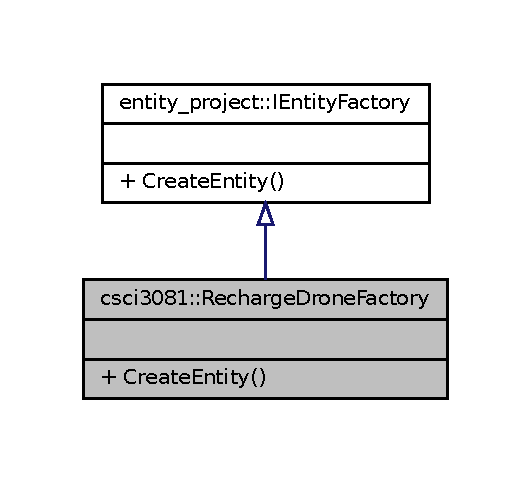
\includegraphics[width=255pt]{classcsci3081_1_1RechargeDroneFactory__inherit__graph}
\end{center}
\end{figure}
\subsection*{Public Member Functions}
\begin{DoxyCompactItemize}
\item 
\hyperlink{classentity__project_1_1IEntity}{I\+Entity} $\ast$ \hyperlink{classcsci3081_1_1RechargeDroneFactory_ab6da0dbaa91fb44d3ae1ebaefeb07091}{Create\+Entity} (const picojson\+::object \&val)
\begin{DoxyCompactList}\small\item\em This is an inheritance function from I\+Entity\+Factory to create an appropriate Entity object based on the argument pass in Given the picojson\+::object val, this should create an entity. Based on the type of entity, there may be different fields. You can see the vals that will be passed in the project/web/scenes directory. Some of the fields are for our backend system and you don\textquotesingle{}t need to worry about them. (for instance, mesh, rotation, offset, etc.) Some fields in val that you will need to create the entity correctly\+: \end{DoxyCompactList}\end{DoxyCompactItemize}


\subsection{Detailed Description}
This is the R\+E\+C\+H\+A\+R\+G\+E\+\_\+\+D\+R\+O\+N\+E\+\_\+\+F\+A\+C\+T\+O\+RY, responsible for making Recharge Drones. 

\subsection{Member Function Documentation}
\mbox{\Hypertarget{classcsci3081_1_1RechargeDroneFactory_ab6da0dbaa91fb44d3ae1ebaefeb07091}\label{classcsci3081_1_1RechargeDroneFactory_ab6da0dbaa91fb44d3ae1ebaefeb07091}} 
\index{csci3081\+::\+Recharge\+Drone\+Factory@{csci3081\+::\+Recharge\+Drone\+Factory}!Create\+Entity@{Create\+Entity}}
\index{Create\+Entity@{Create\+Entity}!csci3081\+::\+Recharge\+Drone\+Factory@{csci3081\+::\+Recharge\+Drone\+Factory}}
\subsubsection{\texorpdfstring{Create\+Entity()}{CreateEntity()}}
{\footnotesize\ttfamily \hyperlink{classentity__project_1_1IEntity}{I\+Entity} $\ast$ csci3081\+::\+Recharge\+Drone\+Factory\+::\+Create\+Entity (\begin{DoxyParamCaption}\item[{const picojson\+::object \&}]{val }\end{DoxyParamCaption})\hspace{0.3cm}{\ttfamily [virtual]}}



This is an inheritance function from I\+Entity\+Factory to create an appropriate Entity object based on the argument pass in Given the picojson\+::object val, this should create an entity. Based on the type of entity, there may be different fields. You can see the vals that will be passed in the project/web/scenes directory. Some of the fields are for our backend system and you don\textquotesingle{}t need to worry about them. (for instance, mesh, rotation, offset, etc.) Some fields in val that you will need to create the entity correctly\+: 

type\+: string (could be \char`\"{}drone/customer/package\char`\"{})

name\+: string

position\+: array (contains \mbox{[}x\+\_\+position, y\+\_\+position, z\+\_\+position\mbox{]})

direction\+: array (contains \mbox{[}x, y, z\mbox{]})


\begin{DoxyParams}[1]{Parameters}
\mbox{\tt in}  & {\em val} & the picojson\+::object that constains all of the necessary information above in a json format \\
\hline
\end{DoxyParams}
\begin{DoxyReturn}{Returns}
I\+Entity pointer if the object has type \char`\"{}recharge\+\_\+drone\char`\"{}; N\+U\+LL otherwise 
\end{DoxyReturn}


Implements \hyperlink{classentity__project_1_1IEntityFactory_ac4e8eaf4294958fef0b98bd3684704bb}{entity\+\_\+project\+::\+I\+Entity\+Factory}.



The documentation for this class was generated from the following files\+:\begin{DoxyCompactItemize}
\item 
/home/user/repo/project/include/\hyperlink{recharge__drone__factory_8h}{recharge\+\_\+drone\+\_\+factory.\+h}\item 
/home/user/repo/project/src/recharge\+\_\+drone\+\_\+factory.\+cc\end{DoxyCompactItemize}

\hypertarget{classcsci3081_1_1Robot}{}\section{csci3081\+:\+:Robot Class Reference}
\label{classcsci3081_1_1Robot}\index{csci3081\+::\+Robot@{csci3081\+::\+Robot}}


A representation of a robot It stores the robot\textquotesingle{}s name, ID, version, position, direction, speed, and dynamic mode.  




{\ttfamily \#include $<$robot.\+h$>$}



Inheritance diagram for csci3081\+:\+:Robot\+:
\nopagebreak
\begin{figure}[H]
\begin{center}
\leavevmode
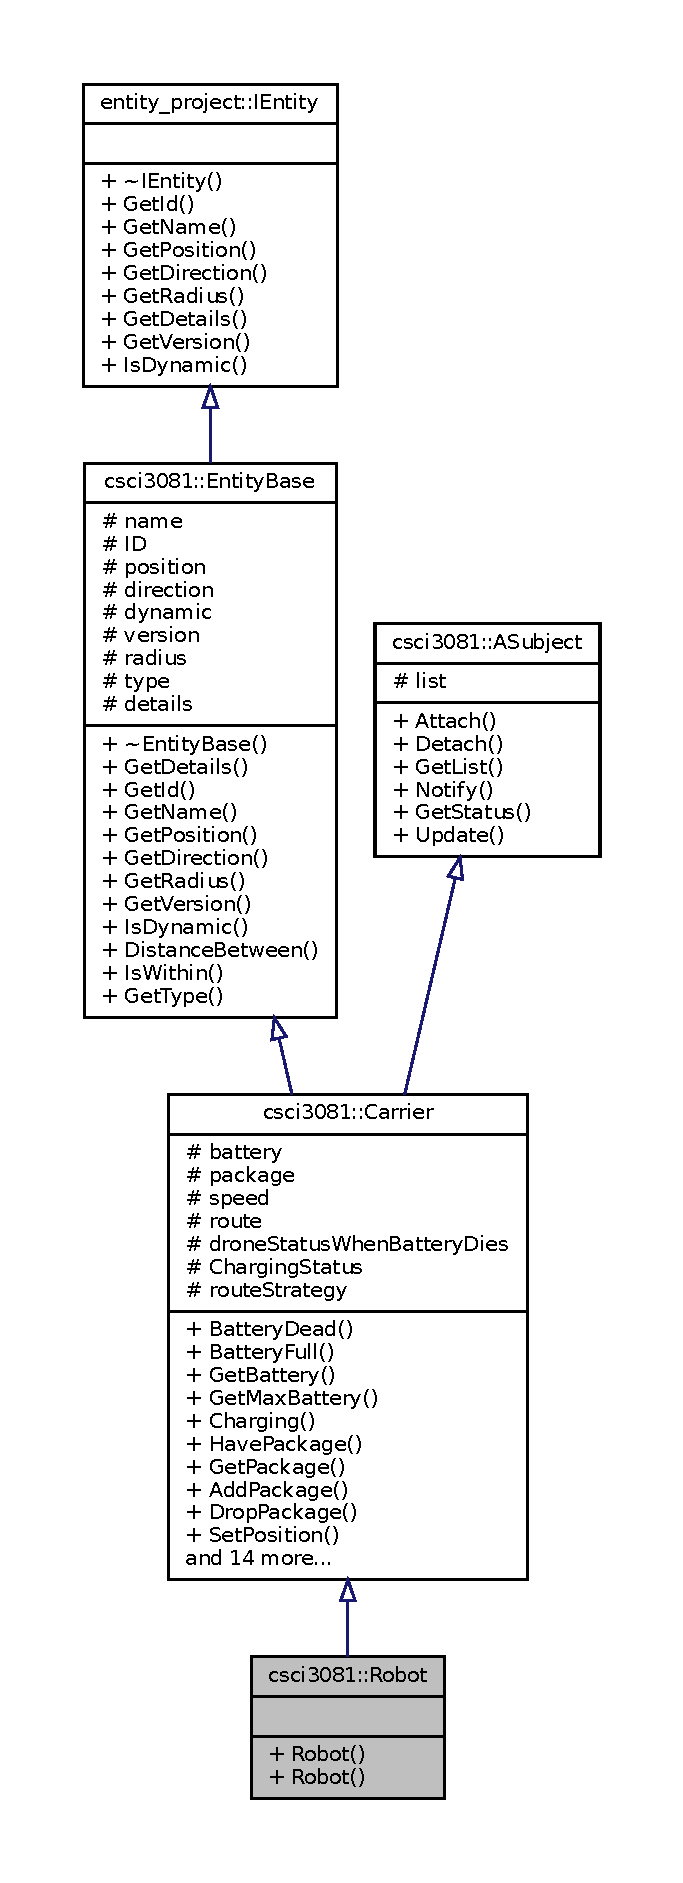
\includegraphics[height=550pt]{classcsci3081_1_1Robot__inherit__graph}
\end{center}
\end{figure}
\subsection*{Public Member Functions}
\begin{DoxyCompactItemize}
\item 
\hyperlink{classcsci3081_1_1Robot_a71e09d18de743a5b677204af60071b4a}{Robot} (const picojson\+::object \&val)
\item 
\hyperlink{classcsci3081_1_1Robot_ae87d6490b70cce02a195794a3bb65b69}{Robot} (\hyperlink{classcsci3081_1_1Robot}{Robot} \&)
\begin{DoxyCompactList}\small\item\em Copy Constructor. This creates a new instance of \hyperlink{classcsci3081_1_1Package}{Package} that has the same content as the \hyperlink{classcsci3081_1_1Package}{Package} argument. \end{DoxyCompactList}\end{DoxyCompactItemize}
\subsection*{Additional Inherited Members}


\subsection{Detailed Description}
A representation of a robot It stores the robot\textquotesingle{}s name, ID, version, position, direction, speed, and dynamic mode. 

\subsection{Constructor \& Destructor Documentation}
\mbox{\Hypertarget{classcsci3081_1_1Robot_a71e09d18de743a5b677204af60071b4a}\label{classcsci3081_1_1Robot_a71e09d18de743a5b677204af60071b4a}} 
\index{csci3081\+::\+Robot@{csci3081\+::\+Robot}!Robot@{Robot}}
\index{Robot@{Robot}!csci3081\+::\+Robot@{csci3081\+::\+Robot}}
\subsubsection{\texorpdfstring{Robot()}{Robot()}\hspace{0.1cm}{\footnotesize\ttfamily [1/2]}}
{\footnotesize\ttfamily csci3081\+::\+Robot\+::\+Robot (\begin{DoxyParamCaption}\item[{const picojson\+::object \&}]{val }\end{DoxyParamCaption})}

Constructor, creates a \hyperlink{classcsci3081_1_1Package}{Package} object param\mbox{[}in\mbox{]} val a picojson\+::object object that has the detail of the package including name, position, direction, radius, and speed \mbox{\Hypertarget{classcsci3081_1_1Robot_ae87d6490b70cce02a195794a3bb65b69}\label{classcsci3081_1_1Robot_ae87d6490b70cce02a195794a3bb65b69}} 
\index{csci3081\+::\+Robot@{csci3081\+::\+Robot}!Robot@{Robot}}
\index{Robot@{Robot}!csci3081\+::\+Robot@{csci3081\+::\+Robot}}
\subsubsection{\texorpdfstring{Robot()}{Robot()}\hspace{0.1cm}{\footnotesize\ttfamily [2/2]}}
{\footnotesize\ttfamily csci3081\+::\+Robot\+::\+Robot (\begin{DoxyParamCaption}\item[{\hyperlink{classcsci3081_1_1Robot}{Robot} \&}]{cpy }\end{DoxyParamCaption})}



Copy Constructor. This creates a new instance of \hyperlink{classcsci3081_1_1Package}{Package} that has the same content as the \hyperlink{classcsci3081_1_1Package}{Package} argument. 


\begin{DoxyParams}[1]{Parameters}
\mbox{\tt in}  & {\em cpy} & \hyperlink{classcsci3081_1_1Robot}{Robot} instance that wants to be copied \\
\hline
\end{DoxyParams}


The documentation for this class was generated from the following files\+:\begin{DoxyCompactItemize}
\item 
/home/user/repo/project/include/\hyperlink{robot_8h}{robot.\+h}\item 
/home/user/repo/project/src/robot.\+cc\end{DoxyCompactItemize}

\hypertarget{classcsci3081_1_1RobotFactory}{}\section{csci3081\+:\+:Robot\+Factory Class Reference}
\label{classcsci3081_1_1RobotFactory}\index{csci3081\+::\+Robot\+Factory@{csci3081\+::\+Robot\+Factory}}


This is the \hyperlink{classcsci3081_1_1RobotFactory}{Robot\+Factory}, responsible for making a robot object.  




{\ttfamily \#include $<$robot\+\_\+factory.\+h$>$}



Inheritance diagram for csci3081\+:\+:Robot\+Factory\+:
\nopagebreak
\begin{figure}[H]
\begin{center}
\leavevmode
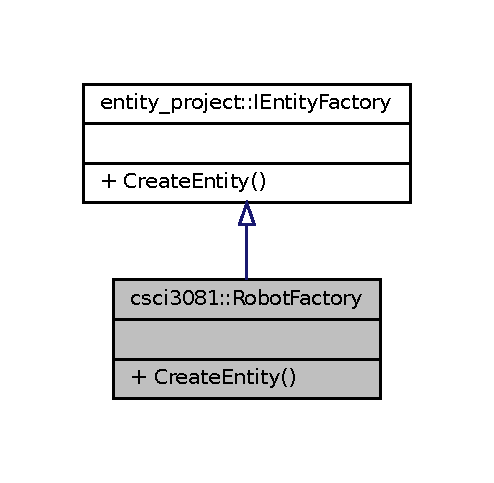
\includegraphics[width=237pt]{classcsci3081_1_1RobotFactory__inherit__graph}
\end{center}
\end{figure}
\subsection*{Public Member Functions}
\begin{DoxyCompactItemize}
\item 
\hyperlink{classentity__project_1_1IEntity}{I\+Entity} $\ast$ \hyperlink{classcsci3081_1_1RobotFactory_a5775ecc230c01ae455284cd04f491129}{Create\+Entity} (const picojson\+::object \&val)
\begin{DoxyCompactList}\small\item\em This is an inheritance function from I\+Entity\+Factory to create an approxiate Entity object based on the argument pass in Given the picojson\+::object val, this should create an entity. Based on the type of entity, there may be different fields. You can see the vals that will be passed in the project/web/scenes directory. Some of the fields are for our backend system and you don\textquotesingle{}t need to worry about them. (for instance, mesh, rotation, offset, etc.) \end{DoxyCompactList}\end{DoxyCompactItemize}


\subsection{Detailed Description}
This is the \hyperlink{classcsci3081_1_1RobotFactory}{Robot\+Factory}, responsible for making a robot object. 

\subsection{Member Function Documentation}
\mbox{\Hypertarget{classcsci3081_1_1RobotFactory_a5775ecc230c01ae455284cd04f491129}\label{classcsci3081_1_1RobotFactory_a5775ecc230c01ae455284cd04f491129}} 
\index{csci3081\+::\+Robot\+Factory@{csci3081\+::\+Robot\+Factory}!Create\+Entity@{Create\+Entity}}
\index{Create\+Entity@{Create\+Entity}!csci3081\+::\+Robot\+Factory@{csci3081\+::\+Robot\+Factory}}
\subsubsection{\texorpdfstring{Create\+Entity()}{CreateEntity()}}
{\footnotesize\ttfamily \hyperlink{classentity__project_1_1IEntity}{I\+Entity} $\ast$ csci3081\+::\+Robot\+Factory\+::\+Create\+Entity (\begin{DoxyParamCaption}\item[{const picojson\+::object \&}]{val }\end{DoxyParamCaption})\hspace{0.3cm}{\ttfamily [virtual]}}



This is an inheritance function from I\+Entity\+Factory to create an approxiate Entity object based on the argument pass in Given the picojson\+::object val, this should create an entity. Based on the type of entity, there may be different fields. You can see the vals that will be passed in the project/web/scenes directory. Some of the fields are for our backend system and you don\textquotesingle{}t need to worry about them. (for instance, mesh, rotation, offset, etc.) 

Some fields in val that you will need to create the entity correctly\+:

type\+: string (could be \char`\"{}robot/drone/customer/package/robot\char`\"{})

name\+: string

position\+: array (contains \mbox{[}x\+\_\+position, y\+\_\+position, z\+\_\+position\mbox{]})

direction\+: array (contains \mbox{[}x, y, z\mbox{]})

speed\+: float

battery\+\_\+capacity\+: float 
\begin{DoxyParams}[1]{Parameters}
\mbox{\tt in}  & {\em val} & the picojson\+::object that constains all of the necessary information above in a json format \\
\hline
\end{DoxyParams}
\begin{DoxyReturn}{Returns}
I\+Entity pointer if the object has type \char`\"{}robot\char`\"{}; N\+U\+LL otherwise 
\end{DoxyReturn}


Implements \hyperlink{classentity__project_1_1IEntityFactory_ac4e8eaf4294958fef0b98bd3684704bb}{entity\+\_\+project\+::\+I\+Entity\+Factory}.



The documentation for this class was generated from the following files\+:\begin{DoxyCompactItemize}
\item 
/home/user/repo/project/include/\hyperlink{robot__factory_8h}{robot\+\_\+factory.\+h}\item 
/home/user/repo/project/src/robot\+\_\+factory.\+cc\end{DoxyCompactItemize}

\hypertarget{classcsci3081_1_1RouteStrategy}{}\section{csci3081\+:\+:Route\+Strategy Class Reference}
\label{classcsci3081_1_1RouteStrategy}\index{csci3081\+::\+Route\+Strategy@{csci3081\+::\+Route\+Strategy}}


This is the Route Strategy class where we can use the interface to decide which type of route behaviour to implement using a strategy pattern.  




{\ttfamily \#include $<$route\+\_\+strategy.\+h$>$}



Inheritance diagram for csci3081\+:\+:Route\+Strategy\+:
\nopagebreak
\begin{figure}[H]
\begin{center}
\leavevmode
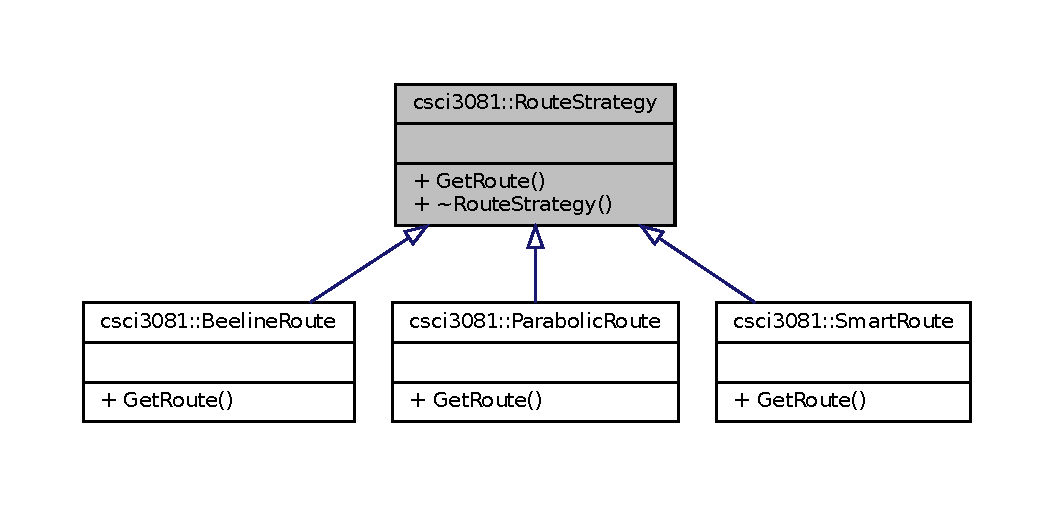
\includegraphics[width=350pt]{classcsci3081_1_1RouteStrategy__inherit__graph}
\end{center}
\end{figure}
\subsection*{Public Member Functions}
\begin{DoxyCompactItemize}
\item 
virtual std\+::vector$<$ std\+::vector$<$ float $>$ $>$ \hyperlink{classcsci3081_1_1RouteStrategy_a4bf67b185a4446324ebc13c1cda40cfe}{Get\+Route} (const \hyperlink{classentity__project_1_1IGraph}{I\+Graph} $\ast$graph, std\+::vector$<$ float $>$ location, std\+::vector$<$ float $>$ dest)=0
\begin{DoxyCompactList}\small\item\em Pure virtual function that will be overridden in derived classes. This function allows the moving item to get the desired route. \end{DoxyCompactList}\end{DoxyCompactItemize}


\subsection{Detailed Description}
This is the Route Strategy class where we can use the interface to decide which type of route behaviour to implement using a strategy pattern. 

\subsection{Member Function Documentation}
\mbox{\Hypertarget{classcsci3081_1_1RouteStrategy_a4bf67b185a4446324ebc13c1cda40cfe}\label{classcsci3081_1_1RouteStrategy_a4bf67b185a4446324ebc13c1cda40cfe}} 
\index{csci3081\+::\+Route\+Strategy@{csci3081\+::\+Route\+Strategy}!Get\+Route@{Get\+Route}}
\index{Get\+Route@{Get\+Route}!csci3081\+::\+Route\+Strategy@{csci3081\+::\+Route\+Strategy}}
\subsubsection{\texorpdfstring{Get\+Route()}{GetRoute()}}
{\footnotesize\ttfamily virtual std\+::vector$<$std\+::vector$<$float$>$ $>$ csci3081\+::\+Route\+Strategy\+::\+Get\+Route (\begin{DoxyParamCaption}\item[{const \hyperlink{classentity__project_1_1IGraph}{I\+Graph} $\ast$}]{graph,  }\item[{std\+::vector$<$ float $>$}]{location,  }\item[{std\+::vector$<$ float $>$}]{dest }\end{DoxyParamCaption})\hspace{0.3cm}{\ttfamily [pure virtual]}}



Pure virtual function that will be overridden in derived classes. This function allows the moving item to get the desired route. 


\begin{DoxyParams}{Parameters}
{\em const} & I\+Graph$\ast$ graph \\
\hline
{\em std\+::vector$<$float$>$} & location \\
\hline
{\em std\+::vector$<$float$>$} & dest \\
\hline
\end{DoxyParams}
\begin{DoxyReturn}{Returns}
std\+::vector $<$std\+::vector$<$float$>$$>$ 
\end{DoxyReturn}


Implemented in \hyperlink{classcsci3081_1_1BeelineRoute_a38aacbeafb14145e807c60990199785c}{csci3081\+::\+Beeline\+Route}, \hyperlink{classcsci3081_1_1ParabolicRoute_adbafff4df041bd49c060578216cb77fc}{csci3081\+::\+Parabolic\+Route}, and \hyperlink{classcsci3081_1_1SmartRoute_a166304ad52fe67131f4540577e3d863d}{csci3081\+::\+Smart\+Route}.



The documentation for this class was generated from the following file\+:\begin{DoxyCompactItemize}
\item 
/home/user/repo/project/include/route\+\_\+strategy.\+h\end{DoxyCompactItemize}

\hypertarget{classcsci3081_1_1SmartRoute}{}\section{csci3081\+:\+:Smart\+Route Class Reference}
\label{classcsci3081_1_1SmartRoute}\index{csci3081\+::\+Smart\+Route@{csci3081\+::\+Smart\+Route}}


This is the Smart Route class where we can use the strategy pattern to implement a A$\ast$ shortest path route.  




{\ttfamily \#include $<$smart\+\_\+route.\+h$>$}



Inheritance diagram for csci3081\+:\+:Smart\+Route\+:
\nopagebreak
\begin{figure}[H]
\begin{center}
\leavevmode
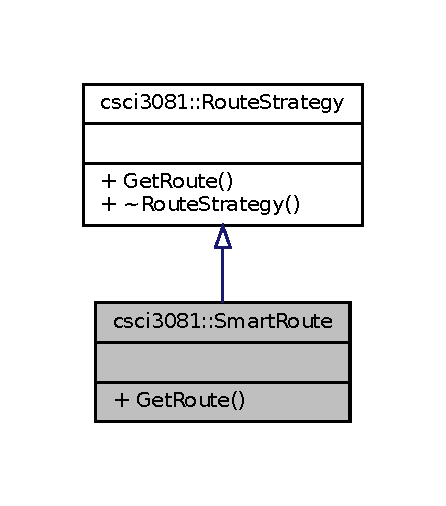
\includegraphics[width=214pt]{classcsci3081_1_1SmartRoute__inherit__graph}
\end{center}
\end{figure}
\subsection*{Public Member Functions}
\begin{DoxyCompactItemize}
\item 
std\+::vector$<$ std\+::vector$<$ float $>$ $>$ \hyperlink{classcsci3081_1_1SmartRoute_a166304ad52fe67131f4540577e3d863d}{Get\+Route} (const \hyperlink{classentity__project_1_1IGraph}{I\+Graph} $\ast$graph, std\+::vector$<$ float $>$ location, std\+::vector$<$ float $>$ dest)
\begin{DoxyCompactList}\small\item\em This function allows the moving item to get the desired route. In this class, the function will return a route that follows the A$\ast$ shortest path smart route. \end{DoxyCompactList}\end{DoxyCompactItemize}


\subsection{Detailed Description}
This is the Smart Route class where we can use the strategy pattern to implement a A$\ast$ shortest path route. 

\subsection{Member Function Documentation}
\mbox{\Hypertarget{classcsci3081_1_1SmartRoute_a166304ad52fe67131f4540577e3d863d}\label{classcsci3081_1_1SmartRoute_a166304ad52fe67131f4540577e3d863d}} 
\index{csci3081\+::\+Smart\+Route@{csci3081\+::\+Smart\+Route}!Get\+Route@{Get\+Route}}
\index{Get\+Route@{Get\+Route}!csci3081\+::\+Smart\+Route@{csci3081\+::\+Smart\+Route}}
\subsubsection{\texorpdfstring{Get\+Route()}{GetRoute()}}
{\footnotesize\ttfamily std\+::vector$<$ std\+::vector$<$ float $>$ $>$ csci3081\+::\+Smart\+Route\+::\+Get\+Route (\begin{DoxyParamCaption}\item[{const \hyperlink{classentity__project_1_1IGraph}{I\+Graph} $\ast$}]{graph,  }\item[{std\+::vector$<$ float $>$}]{location,  }\item[{std\+::vector$<$ float $>$}]{dest }\end{DoxyParamCaption})\hspace{0.3cm}{\ttfamily [virtual]}}



This function allows the moving item to get the desired route. In this class, the function will return a route that follows the A$\ast$ shortest path smart route. 


\begin{DoxyParams}{Parameters}
{\em const} & I\+Graph$\ast$ graph \\
\hline
{\em std\+::vector$<$float$>$} & location \\
\hline
{\em std\+::vector$<$float$>$} & dest \\
\hline
\end{DoxyParams}
\begin{DoxyReturn}{Returns}
std\+::vector $<$std\+::vector$<$float$>$$>$ 
\end{DoxyReturn}


Implements \hyperlink{classcsci3081_1_1RouteStrategy_a4bf67b185a4446324ebc13c1cda40cfe}{csci3081\+::\+Route\+Strategy}.



The documentation for this class was generated from the following files\+:\begin{DoxyCompactItemize}
\item 
/home/user/repo/project/include/smart\+\_\+route.\+h\item 
/home/user/repo/project/src/smart\+\_\+route.\+cc\end{DoxyCompactItemize}

\hypertarget{classcsci3081_1_1Vector}{}\section{csci3081\+:\+:Vector Class Reference}
\label{classcsci3081_1_1Vector}\index{csci3081\+::\+Vector@{csci3081\+::\+Vector}}


This is the interface class for the \hyperlink{classcsci3081_1_1Vector3D}{Vector3D} and \hyperlink{classcsci3081_1_1Vector2D}{Vector2D} classes.  




{\ttfamily \#include $<$vector.\+h$>$}



Inheritance diagram for csci3081\+:\+:Vector\+:
\nopagebreak
\begin{figure}[H]
\begin{center}
\leavevmode
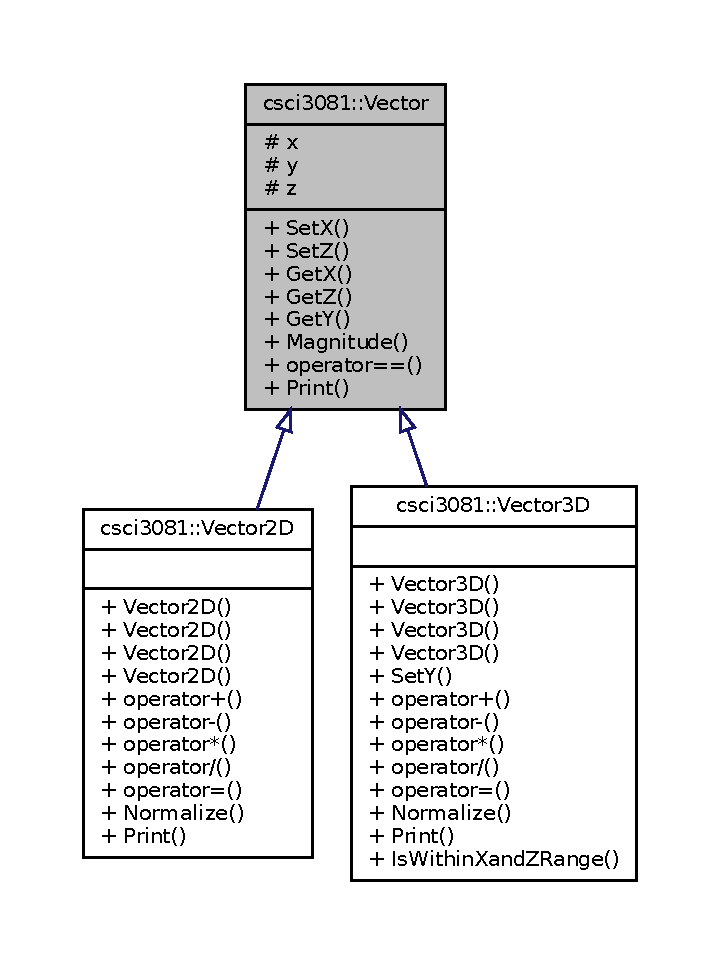
\includegraphics[width=346pt]{classcsci3081_1_1Vector__inherit__graph}
\end{center}
\end{figure}
\subsection*{Public Member Functions}
\begin{DoxyCompactItemize}
\item 
\mbox{\Hypertarget{classcsci3081_1_1Vector_a25668daef8abbefe545400b61370e465}\label{classcsci3081_1_1Vector_a25668daef8abbefe545400b61370e465}} 
void \hyperlink{classcsci3081_1_1Vector_a25668daef8abbefe545400b61370e465}{SetX} (float x\+\_\+)
\begin{DoxyCompactList}\small\item\em This function uses to set x coordinator of a vector instance. \end{DoxyCompactList}\item 
\mbox{\Hypertarget{classcsci3081_1_1Vector_ade27e84fb7cfc517d10982a231cf1514}\label{classcsci3081_1_1Vector_ade27e84fb7cfc517d10982a231cf1514}} 
void \hyperlink{classcsci3081_1_1Vector_ade27e84fb7cfc517d10982a231cf1514}{SetZ} (float z\+\_\+)
\begin{DoxyCompactList}\small\item\em This function uses to set z coordinator of a vector instance. \end{DoxyCompactList}\item 
\mbox{\Hypertarget{classcsci3081_1_1Vector_a22a861b6ac42caa61304da2f291eccff}\label{classcsci3081_1_1Vector_a22a861b6ac42caa61304da2f291eccff}} 
float \hyperlink{classcsci3081_1_1Vector_a22a861b6ac42caa61304da2f291eccff}{GetX} () const
\begin{DoxyCompactList}\small\item\em This function uses to get x coordinator of a vector instance. \end{DoxyCompactList}\item 
\mbox{\Hypertarget{classcsci3081_1_1Vector_a3e4a88cae4754e20f214a3029a8831dd}\label{classcsci3081_1_1Vector_a3e4a88cae4754e20f214a3029a8831dd}} 
float \hyperlink{classcsci3081_1_1Vector_a3e4a88cae4754e20f214a3029a8831dd}{GetZ} () const
\begin{DoxyCompactList}\small\item\em This function uses to get z coordinator of a vector instance. \end{DoxyCompactList}\item 
\mbox{\Hypertarget{classcsci3081_1_1Vector_aeefa39719f335e798a9475f7f9cf8ca7}\label{classcsci3081_1_1Vector_aeefa39719f335e798a9475f7f9cf8ca7}} 
float \hyperlink{classcsci3081_1_1Vector_aeefa39719f335e798a9475f7f9cf8ca7}{GetY} () const
\begin{DoxyCompactList}\small\item\em This function uses to get y coordinator of a vector instance. \end{DoxyCompactList}\item 
\mbox{\Hypertarget{classcsci3081_1_1Vector_af9e09e9b9ce246fe42907c78533d3dc4}\label{classcsci3081_1_1Vector_af9e09e9b9ce246fe42907c78533d3dc4}} 
float \hyperlink{classcsci3081_1_1Vector_af9e09e9b9ce246fe42907c78533d3dc4}{Magnitude} ()
\begin{DoxyCompactList}\small\item\em This function returns the magitude of a vector instance. \end{DoxyCompactList}\item 
bool \hyperlink{classcsci3081_1_1Vector_a0ce4762325d81521ba1e1a1f6ee1a171}{operator==} (const \hyperlink{classcsci3081_1_1Vector}{Vector} \&)
\begin{DoxyCompactList}\small\item\em Convert vector distance to std\+::vector$<$float$>$ instances. \end{DoxyCompactList}\item 
\mbox{\Hypertarget{classcsci3081_1_1Vector_a8f0661975d9635c803551cd778f75ed4}\label{classcsci3081_1_1Vector_a8f0661975d9635c803551cd778f75ed4}} 
virtual void \hyperlink{classcsci3081_1_1Vector_a8f0661975d9635c803551cd778f75ed4}{Print} ()=0
\begin{DoxyCompactList}\small\item\em Function to print the coordinate of a vector instance. \end{DoxyCompactList}\end{DoxyCompactItemize}
\subsection*{Protected Attributes}
\begin{DoxyCompactItemize}
\item 
\mbox{\Hypertarget{classcsci3081_1_1Vector_aad8fb83cdb7c74bec16148252a30ef85}\label{classcsci3081_1_1Vector_aad8fb83cdb7c74bec16148252a30ef85}} 
float {\bfseries x}
\item 
\mbox{\Hypertarget{classcsci3081_1_1Vector_a4636a264c229f016fcca5b066d6b2329}\label{classcsci3081_1_1Vector_a4636a264c229f016fcca5b066d6b2329}} 
float {\bfseries y}
\item 
\mbox{\Hypertarget{classcsci3081_1_1Vector_a11acb4af7109f0f16cec3eb95c881128}\label{classcsci3081_1_1Vector_a11acb4af7109f0f16cec3eb95c881128}} 
float \hyperlink{classcsci3081_1_1Vector_a11acb4af7109f0f16cec3eb95c881128}{z}
\begin{DoxyCompactList}\small\item\em Coordinates of a vector. \end{DoxyCompactList}\end{DoxyCompactItemize}
\subsection*{Friends}
\begin{DoxyCompactItemize}
\item 
float \hyperlink{classcsci3081_1_1Vector_ae3bcd7cf17dbea6b1f935534c69ca0f0}{Dot\+Product} (const \hyperlink{classcsci3081_1_1Vector}{Vector} \&v1, const \hyperlink{classcsci3081_1_1Vector}{Vector} \&v2)
\begin{DoxyCompactList}\small\item\em Compute the dot product (float variable) between two vectors instances. \end{DoxyCompactList}\item 
float \hyperlink{classcsci3081_1_1Vector_acd23c5473c105b42b0656eaa0ffa02d2}{Distance} (const \hyperlink{classcsci3081_1_1Vector}{Vector} \&v1, const \hyperlink{classcsci3081_1_1Vector}{Vector} \&v2)
\begin{DoxyCompactList}\small\item\em Compute the distance (float variable) between two vectors instances. \end{DoxyCompactList}\item 
std\+::vector$<$ float $>$ \hyperlink{classcsci3081_1_1Vector_a7647fb9682b28785ce754fa445a2d365}{to\+Vector\+Float} (\hyperlink{classcsci3081_1_1Vector}{Vector} \&v)
\begin{DoxyCompactList}\small\item\em Convert vector distance to std\+::vector$<$float$>$ instances. \end{DoxyCompactList}\end{DoxyCompactItemize}


\subsection{Detailed Description}
This is the interface class for the \hyperlink{classcsci3081_1_1Vector3D}{Vector3D} and \hyperlink{classcsci3081_1_1Vector2D}{Vector2D} classes. 

This class will set up (virtual) common methods as well as attributes shared by both \hyperlink{classcsci3081_1_1Vector3D}{Vector3D} and vector2D class. Also has some friends functions to find relationship between more than one vector instances 

\subsection{Member Function Documentation}
\mbox{\Hypertarget{classcsci3081_1_1Vector_a0ce4762325d81521ba1e1a1f6ee1a171}\label{classcsci3081_1_1Vector_a0ce4762325d81521ba1e1a1f6ee1a171}} 
\index{csci3081\+::\+Vector@{csci3081\+::\+Vector}!operator==@{operator==}}
\index{operator==@{operator==}!csci3081\+::\+Vector@{csci3081\+::\+Vector}}
\subsubsection{\texorpdfstring{operator==()}{operator==()}}
{\footnotesize\ttfamily bool csci3081\+::\+Vector\+::operator== (\begin{DoxyParamCaption}\item[{const \hyperlink{classcsci3081_1_1Vector}{Vector} \&}]{other }\end{DoxyParamCaption})}



Convert vector distance to std\+::vector$<$float$>$ instances. 


\begin{DoxyParams}[1]{Parameters}
\mbox{\tt in}  & {\em v} & \hyperlink{classcsci3081_1_1Vector}{Vector} instance \\
\hline
\end{DoxyParams}
\begin{DoxyReturn}{Returns}
True if argument vector is equal to current object False otherwise 
\end{DoxyReturn}


\subsection{Friends And Related Function Documentation}
\mbox{\Hypertarget{classcsci3081_1_1Vector_acd23c5473c105b42b0656eaa0ffa02d2}\label{classcsci3081_1_1Vector_acd23c5473c105b42b0656eaa0ffa02d2}} 
\index{csci3081\+::\+Vector@{csci3081\+::\+Vector}!Distance@{Distance}}
\index{Distance@{Distance}!csci3081\+::\+Vector@{csci3081\+::\+Vector}}
\subsubsection{\texorpdfstring{Distance}{Distance}}
{\footnotesize\ttfamily float Distance (\begin{DoxyParamCaption}\item[{const \hyperlink{classcsci3081_1_1Vector}{Vector} \&}]{v1,  }\item[{const \hyperlink{classcsci3081_1_1Vector}{Vector} \&}]{v2 }\end{DoxyParamCaption})\hspace{0.3cm}{\ttfamily [friend]}}



Compute the distance (float variable) between two vectors instances. 


\begin{DoxyParams}[1]{Parameters}
\mbox{\tt in}  & {\em v1} & \hyperlink{classcsci3081_1_1Vector}{Vector} instance \\
\hline
\mbox{\tt in}  & {\em v2} & \hyperlink{classcsci3081_1_1Vector}{Vector} instance \\
\hline
\end{DoxyParams}
\begin{DoxyReturn}{Returns}
float Distance of v1 and v2 
\end{DoxyReturn}
\mbox{\Hypertarget{classcsci3081_1_1Vector_ae3bcd7cf17dbea6b1f935534c69ca0f0}\label{classcsci3081_1_1Vector_ae3bcd7cf17dbea6b1f935534c69ca0f0}} 
\index{csci3081\+::\+Vector@{csci3081\+::\+Vector}!Dot\+Product@{Dot\+Product}}
\index{Dot\+Product@{Dot\+Product}!csci3081\+::\+Vector@{csci3081\+::\+Vector}}
\subsubsection{\texorpdfstring{Dot\+Product}{DotProduct}}
{\footnotesize\ttfamily float Dot\+Product (\begin{DoxyParamCaption}\item[{const \hyperlink{classcsci3081_1_1Vector}{Vector} \&}]{v1,  }\item[{const \hyperlink{classcsci3081_1_1Vector}{Vector} \&}]{v2 }\end{DoxyParamCaption})\hspace{0.3cm}{\ttfamily [friend]}}



Compute the dot product (float variable) between two vectors instances. 


\begin{DoxyParams}[1]{Parameters}
\mbox{\tt in}  & {\em v1} & \hyperlink{classcsci3081_1_1Vector}{Vector} instance \\
\hline
\mbox{\tt in}  & {\em v2} & \hyperlink{classcsci3081_1_1Vector}{Vector} instance \\
\hline
\end{DoxyParams}
\begin{DoxyReturn}{Returns}
float Dot product of v1 and v2 
\end{DoxyReturn}
\mbox{\Hypertarget{classcsci3081_1_1Vector_a7647fb9682b28785ce754fa445a2d365}\label{classcsci3081_1_1Vector_a7647fb9682b28785ce754fa445a2d365}} 
\index{csci3081\+::\+Vector@{csci3081\+::\+Vector}!to\+Vector\+Float@{to\+Vector\+Float}}
\index{to\+Vector\+Float@{to\+Vector\+Float}!csci3081\+::\+Vector@{csci3081\+::\+Vector}}
\subsubsection{\texorpdfstring{to\+Vector\+Float}{toVectorFloat}}
{\footnotesize\ttfamily std\+::vector$<$float$>$ to\+Vector\+Float (\begin{DoxyParamCaption}\item[{\hyperlink{classcsci3081_1_1Vector}{Vector} \&}]{v }\end{DoxyParamCaption})\hspace{0.3cm}{\ttfamily [friend]}}



Convert vector distance to std\+::vector$<$float$>$ instances. 


\begin{DoxyParams}[1]{Parameters}
\mbox{\tt in}  & {\em v} & \hyperlink{classcsci3081_1_1Vector}{Vector} instance \\
\hline
\end{DoxyParams}
\begin{DoxyReturn}{Returns}
std\+::vector$<$float$>$ Have x,y,z as its elements 
\end{DoxyReturn}


The documentation for this class was generated from the following files\+:\begin{DoxyCompactItemize}
\item 
/home/user/repo/project/include/\hyperlink{vector_8h}{vector.\+h}\item 
/home/user/repo/project/src/vector.\+cc\end{DoxyCompactItemize}

\hypertarget{classcsci3081_1_1Vector2D}{}\section{csci3081\+:\+:Vector2D Class Reference}
\label{classcsci3081_1_1Vector2D}\index{csci3081\+::\+Vector2D@{csci3081\+::\+Vector2D}}


This is the \hyperlink{classcsci3081_1_1Vector2D}{Vector2D} class.  




{\ttfamily \#include $<$vector.\+h$>$}



Inheritance diagram for csci3081\+:\+:Vector2D\+:
\nopagebreak
\begin{figure}[H]
\begin{center}
\leavevmode
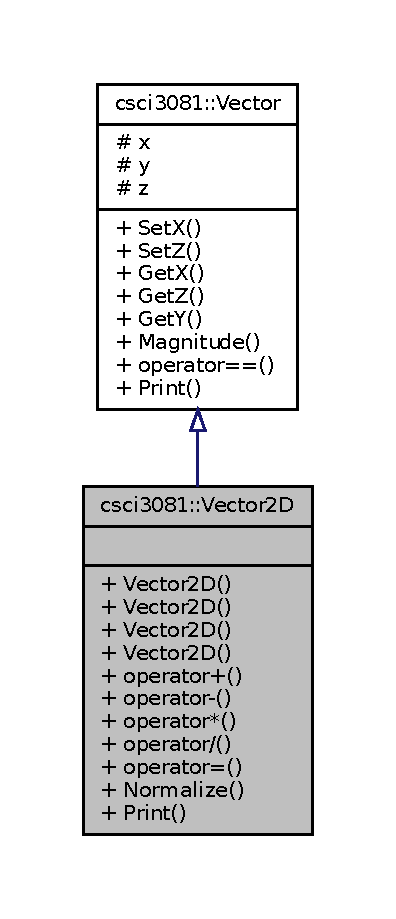
\includegraphics[width=190pt]{classcsci3081_1_1Vector2D__inherit__graph}
\end{center}
\end{figure}
\subsection*{Public Member Functions}
\begin{DoxyCompactItemize}
\item 
\mbox{\Hypertarget{classcsci3081_1_1Vector2D_a4fad6fe37d4bc31a4aee9e2a5f32a1e8}\label{classcsci3081_1_1Vector2D_a4fad6fe37d4bc31a4aee9e2a5f32a1e8}} 
\hyperlink{classcsci3081_1_1Vector2D_a4fad6fe37d4bc31a4aee9e2a5f32a1e8}{Vector2D} ()
\begin{DoxyCompactList}\small\item\em Constructor. This sets up an instance of \hyperlink{classcsci3081_1_1Vector2D}{Vector2D} with zero coordinates. \end{DoxyCompactList}\item 
\hyperlink{classcsci3081_1_1Vector2D_a68e2f6906ba36747d914ef4923bee667}{Vector2D} (std\+::vector$<$ float $>$ arg)
\begin{DoxyCompactList}\small\item\em Constructor. This sets up an instance of \hyperlink{classcsci3081_1_1Vector2D}{Vector2D} with 2 coordinates as arguments. \end{DoxyCompactList}\item 
\hyperlink{classcsci3081_1_1Vector2D_a39919ae0bc8a91377c20d26f9201e963}{Vector2D} (float x\+\_\+, float z\+\_\+)
\begin{DoxyCompactList}\small\item\em Constructor. This sets up an instance of \hyperlink{classcsci3081_1_1Vector3D}{Vector3D} with 3 coordinates as arguments. \end{DoxyCompactList}\item 
\hyperlink{classcsci3081_1_1Vector2D_a7e70f495937c305fda255bcf0dfb85a8}{Vector2D} (const \hyperlink{classcsci3081_1_1Vector2D}{Vector2D} \&)
\begin{DoxyCompactList}\small\item\em Copy Constructor. This creates a new instance of \hyperlink{classcsci3081_1_1Vector2D}{Vector2D} that has the same content as the \hyperlink{classcsci3081_1_1Vector2D}{Vector2D} argument. \end{DoxyCompactList}\item 
\hyperlink{classcsci3081_1_1Vector2D}{Vector2D} \hyperlink{classcsci3081_1_1Vector2D_a7431773929a3d0c18ab926eae0e4bc28}{operator+} (const \hyperlink{classcsci3081_1_1Vector2D}{Vector2D} \&)
\begin{DoxyCompactList}\small\item\em overloading operator + to do addition between \hyperlink{classcsci3081_1_1Vector2D}{Vector2D} instances \end{DoxyCompactList}\item 
\hyperlink{classcsci3081_1_1Vector2D}{Vector2D} \hyperlink{classcsci3081_1_1Vector2D_a8ccf17ebee11a2f8f3ce66dd9dec8a13}{operator-\/} (const \hyperlink{classcsci3081_1_1Vector2D}{Vector2D} \&)
\begin{DoxyCompactList}\small\item\em overloading operator -\/ to do addition between \hyperlink{classcsci3081_1_1Vector2D}{Vector2D} instances \end{DoxyCompactList}\item 
\hyperlink{classcsci3081_1_1Vector2D}{Vector2D} \hyperlink{classcsci3081_1_1Vector2D_a73ad5eb3819cfc93eba7d542abf54acf}{operator$\ast$} (float)
\begin{DoxyCompactList}\small\item\em overloading operator $\ast$ to do multiply a \hyperlink{classcsci3081_1_1Vector2D}{Vector2D} instance to a float \end{DoxyCompactList}\item 
\hyperlink{classcsci3081_1_1Vector2D}{Vector2D} \hyperlink{classcsci3081_1_1Vector2D_a9e123abdcebfb672cea47d705604a968}{operator/} (float)
\begin{DoxyCompactList}\small\item\em overloading operator / to do division a \hyperlink{classcsci3081_1_1Vector2D}{Vector2D} instance to a float \end{DoxyCompactList}\item 
\hyperlink{classcsci3081_1_1Vector2D}{Vector2D} \& \hyperlink{classcsci3081_1_1Vector2D_a91ae4915d5eee2fcccf2fedf6d6e7309}{operator=} (const \hyperlink{classcsci3081_1_1Vector2D}{Vector2D} \&)
\begin{DoxyCompactList}\small\item\em overloading operator = to copy one \hyperlink{classcsci3081_1_1Vector2D}{Vector2D} to another \end{DoxyCompactList}\item 
\mbox{\Hypertarget{classcsci3081_1_1Vector2D_a794e9b3fd7a07dc50c823a8fded0b4e1}\label{classcsci3081_1_1Vector2D_a794e9b3fd7a07dc50c823a8fded0b4e1}} 
\hyperlink{classcsci3081_1_1Vector2D}{Vector2D} \hyperlink{classcsci3081_1_1Vector2D_a794e9b3fd7a07dc50c823a8fded0b4e1}{Normalize} ()
\begin{DoxyCompactList}\small\item\em This function normalizes a \hyperlink{classcsci3081_1_1Vector2D}{Vector2D} instance. \end{DoxyCompactList}\item 
void \hyperlink{classcsci3081_1_1Vector2D_af849fc65ec2d153b53884c8de818fae6}{Print} ()
\begin{DoxyCompactList}\small\item\em Function to print the coordinate of a vector instance. \end{DoxyCompactList}\end{DoxyCompactItemize}
\subsection*{Additional Inherited Members}


\subsection{Detailed Description}
This is the \hyperlink{classcsci3081_1_1Vector2D}{Vector2D} class. 

This class instantiates a \hyperlink{classcsci3081_1_1Vector2D}{Vector2D} object and with basic overload math expression that can be done with \hyperlink{classcsci3081_1_1Vector}{Vector} in 2D 

\subsection{Constructor \& Destructor Documentation}
\mbox{\Hypertarget{classcsci3081_1_1Vector2D_a68e2f6906ba36747d914ef4923bee667}\label{classcsci3081_1_1Vector2D_a68e2f6906ba36747d914ef4923bee667}} 
\index{csci3081\+::\+Vector2D@{csci3081\+::\+Vector2D}!Vector2D@{Vector2D}}
\index{Vector2D@{Vector2D}!csci3081\+::\+Vector2D@{csci3081\+::\+Vector2D}}
\subsubsection{\texorpdfstring{Vector2\+D()}{Vector2D()}\hspace{0.1cm}{\footnotesize\ttfamily [1/3]}}
{\footnotesize\ttfamily csci3081\+::\+Vector2\+D\+::\+Vector2D (\begin{DoxyParamCaption}\item[{std\+::vector$<$ float $>$}]{arg }\end{DoxyParamCaption})}



Constructor. This sets up an instance of \hyperlink{classcsci3081_1_1Vector2D}{Vector2D} with 2 coordinates as arguments. 


\begin{DoxyParams}[1]{Parameters}
\mbox{\tt in}  & {\em arg} & std\+::vector$<$float$>$ that stores coordinates \\
\hline
\end{DoxyParams}
\mbox{\Hypertarget{classcsci3081_1_1Vector2D_a39919ae0bc8a91377c20d26f9201e963}\label{classcsci3081_1_1Vector2D_a39919ae0bc8a91377c20d26f9201e963}} 
\index{csci3081\+::\+Vector2D@{csci3081\+::\+Vector2D}!Vector2D@{Vector2D}}
\index{Vector2D@{Vector2D}!csci3081\+::\+Vector2D@{csci3081\+::\+Vector2D}}
\subsubsection{\texorpdfstring{Vector2\+D()}{Vector2D()}\hspace{0.1cm}{\footnotesize\ttfamily [2/3]}}
{\footnotesize\ttfamily csci3081\+::\+Vector2\+D\+::\+Vector2D (\begin{DoxyParamCaption}\item[{float}]{x\+\_\+,  }\item[{float}]{z\+\_\+ }\end{DoxyParamCaption})}



Constructor. This sets up an instance of \hyperlink{classcsci3081_1_1Vector3D}{Vector3D} with 3 coordinates as arguments. 


\begin{DoxyParams}[1]{Parameters}
\mbox{\tt in}  & {\em x\+\_\+} & float, x-\/coordinate \\
\hline
\mbox{\tt in}  & {\em z\+\_\+} & float, z-\/coordinate \\
\hline
\end{DoxyParams}
\mbox{\Hypertarget{classcsci3081_1_1Vector2D_a7e70f495937c305fda255bcf0dfb85a8}\label{classcsci3081_1_1Vector2D_a7e70f495937c305fda255bcf0dfb85a8}} 
\index{csci3081\+::\+Vector2D@{csci3081\+::\+Vector2D}!Vector2D@{Vector2D}}
\index{Vector2D@{Vector2D}!csci3081\+::\+Vector2D@{csci3081\+::\+Vector2D}}
\subsubsection{\texorpdfstring{Vector2\+D()}{Vector2D()}\hspace{0.1cm}{\footnotesize\ttfamily [3/3]}}
{\footnotesize\ttfamily csci3081\+::\+Vector2\+D\+::\+Vector2D (\begin{DoxyParamCaption}\item[{const \hyperlink{classcsci3081_1_1Vector2D}{Vector2D} \&}]{copy }\end{DoxyParamCaption})}



Copy Constructor. This creates a new instance of \hyperlink{classcsci3081_1_1Vector2D}{Vector2D} that has the same content as the \hyperlink{classcsci3081_1_1Vector2D}{Vector2D} argument. 


\begin{DoxyParams}[1]{Parameters}
\mbox{\tt in}  & {\em copy} & \hyperlink{classcsci3081_1_1Vector2D}{Vector2D} instance that wants to be copied \\
\hline
\end{DoxyParams}


\subsection{Member Function Documentation}
\mbox{\Hypertarget{classcsci3081_1_1Vector2D_a73ad5eb3819cfc93eba7d542abf54acf}\label{classcsci3081_1_1Vector2D_a73ad5eb3819cfc93eba7d542abf54acf}} 
\index{csci3081\+::\+Vector2D@{csci3081\+::\+Vector2D}!operator$\ast$@{operator$\ast$}}
\index{operator$\ast$@{operator$\ast$}!csci3081\+::\+Vector2D@{csci3081\+::\+Vector2D}}
\subsubsection{\texorpdfstring{operator$\ast$()}{operator*()}}
{\footnotesize\ttfamily \hyperlink{classcsci3081_1_1Vector2D}{Vector2D} csci3081\+::\+Vector2\+D\+::operator$\ast$ (\begin{DoxyParamCaption}\item[{float}]{other }\end{DoxyParamCaption})}



overloading operator $\ast$ to do multiply a \hyperlink{classcsci3081_1_1Vector2D}{Vector2D} instance to a float 


\begin{DoxyParams}{Parameters}
{\em other} & float factor that want to multiply the \hyperlink{classcsci3081_1_1Vector2D}{Vector2D} with \\
\hline
\end{DoxyParams}
\mbox{\Hypertarget{classcsci3081_1_1Vector2D_a7431773929a3d0c18ab926eae0e4bc28}\label{classcsci3081_1_1Vector2D_a7431773929a3d0c18ab926eae0e4bc28}} 
\index{csci3081\+::\+Vector2D@{csci3081\+::\+Vector2D}!operator+@{operator+}}
\index{operator+@{operator+}!csci3081\+::\+Vector2D@{csci3081\+::\+Vector2D}}
\subsubsection{\texorpdfstring{operator+()}{operator+()}}
{\footnotesize\ttfamily \hyperlink{classcsci3081_1_1Vector2D}{Vector2D} csci3081\+::\+Vector2\+D\+::operator+ (\begin{DoxyParamCaption}\item[{const \hyperlink{classcsci3081_1_1Vector2D}{Vector2D} \&}]{other }\end{DoxyParamCaption})}



overloading operator + to do addition between \hyperlink{classcsci3081_1_1Vector2D}{Vector2D} instances 


\begin{DoxyParams}{Parameters}
{\em other} & the right hand side \hyperlink{classcsci3081_1_1Vector2D}{Vector2D} of the addition \\
\hline
\end{DoxyParams}
\mbox{\Hypertarget{classcsci3081_1_1Vector2D_a8ccf17ebee11a2f8f3ce66dd9dec8a13}\label{classcsci3081_1_1Vector2D_a8ccf17ebee11a2f8f3ce66dd9dec8a13}} 
\index{csci3081\+::\+Vector2D@{csci3081\+::\+Vector2D}!operator-\/@{operator-\/}}
\index{operator-\/@{operator-\/}!csci3081\+::\+Vector2D@{csci3081\+::\+Vector2D}}
\subsubsection{\texorpdfstring{operator-\/()}{operator-()}}
{\footnotesize\ttfamily \hyperlink{classcsci3081_1_1Vector2D}{Vector2D} csci3081\+::\+Vector2\+D\+::operator-\/ (\begin{DoxyParamCaption}\item[{const \hyperlink{classcsci3081_1_1Vector2D}{Vector2D} \&}]{other }\end{DoxyParamCaption})}



overloading operator -\/ to do addition between \hyperlink{classcsci3081_1_1Vector2D}{Vector2D} instances 


\begin{DoxyParams}{Parameters}
{\em other} & the right hand side \hyperlink{classcsci3081_1_1Vector2D}{Vector2D} of the subtraction \\
\hline
\end{DoxyParams}
\mbox{\Hypertarget{classcsci3081_1_1Vector2D_a9e123abdcebfb672cea47d705604a968}\label{classcsci3081_1_1Vector2D_a9e123abdcebfb672cea47d705604a968}} 
\index{csci3081\+::\+Vector2D@{csci3081\+::\+Vector2D}!operator/@{operator/}}
\index{operator/@{operator/}!csci3081\+::\+Vector2D@{csci3081\+::\+Vector2D}}
\subsubsection{\texorpdfstring{operator/()}{operator/()}}
{\footnotesize\ttfamily \hyperlink{classcsci3081_1_1Vector2D}{Vector2D} csci3081\+::\+Vector2\+D\+::operator/ (\begin{DoxyParamCaption}\item[{float}]{other }\end{DoxyParamCaption})}



overloading operator / to do division a \hyperlink{classcsci3081_1_1Vector2D}{Vector2D} instance to a float 


\begin{DoxyParams}{Parameters}
{\em other} & float factor that want to divide the \hyperlink{classcsci3081_1_1Vector2D}{Vector2D} with \\
\hline
\end{DoxyParams}
\mbox{\Hypertarget{classcsci3081_1_1Vector2D_a91ae4915d5eee2fcccf2fedf6d6e7309}\label{classcsci3081_1_1Vector2D_a91ae4915d5eee2fcccf2fedf6d6e7309}} 
\index{csci3081\+::\+Vector2D@{csci3081\+::\+Vector2D}!operator=@{operator=}}
\index{operator=@{operator=}!csci3081\+::\+Vector2D@{csci3081\+::\+Vector2D}}
\subsubsection{\texorpdfstring{operator=()}{operator=()}}
{\footnotesize\ttfamily \hyperlink{classcsci3081_1_1Vector2D}{Vector2D} \& csci3081\+::\+Vector2\+D\+::operator= (\begin{DoxyParamCaption}\item[{const \hyperlink{classcsci3081_1_1Vector2D}{Vector2D} \&}]{cpy }\end{DoxyParamCaption})}



overloading operator = to copy one \hyperlink{classcsci3081_1_1Vector2D}{Vector2D} to another 


\begin{DoxyParams}{Parameters}
{\em cpy} & the \hyperlink{classcsci3081_1_1Vector2D}{Vector2D} object that wants to copy \\
\hline
\end{DoxyParams}
\mbox{\Hypertarget{classcsci3081_1_1Vector2D_af849fc65ec2d153b53884c8de818fae6}\label{classcsci3081_1_1Vector2D_af849fc65ec2d153b53884c8de818fae6}} 
\index{csci3081\+::\+Vector2D@{csci3081\+::\+Vector2D}!Print@{Print}}
\index{Print@{Print}!csci3081\+::\+Vector2D@{csci3081\+::\+Vector2D}}
\subsubsection{\texorpdfstring{Print()}{Print()}}
{\footnotesize\ttfamily void csci3081\+::\+Vector2\+D\+::\+Print (\begin{DoxyParamCaption}{ }\end{DoxyParamCaption})\hspace{0.3cm}{\ttfamily [virtual]}}



Function to print the coordinate of a vector instance. 



Implements \hyperlink{classcsci3081_1_1Vector_a8f0661975d9635c803551cd778f75ed4}{csci3081\+::\+Vector}.



The documentation for this class was generated from the following files\+:\begin{DoxyCompactItemize}
\item 
/home/user/repo/project/include/\hyperlink{vector_8h}{vector.\+h}\item 
/home/user/repo/project/src/vector.\+cc\end{DoxyCompactItemize}

\hypertarget{classcsci3081_1_1Vector3D}{}\section{csci3081\+:\+:Vector3D Class Reference}
\label{classcsci3081_1_1Vector3D}\index{csci3081\+::\+Vector3D@{csci3081\+::\+Vector3D}}


This is the \hyperlink{classcsci3081_1_1Vector3D}{Vector3D} class.  




{\ttfamily \#include $<$vector.\+h$>$}



Inheritance diagram for csci3081\+:\+:Vector3D\+:
\nopagebreak
\begin{figure}[H]
\begin{center}
\leavevmode
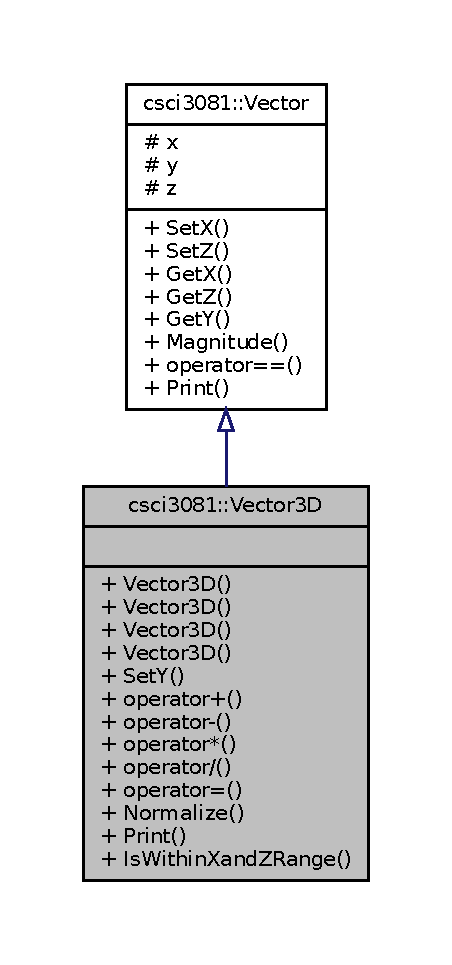
\includegraphics[width=217pt]{classcsci3081_1_1Vector3D__inherit__graph}
\end{center}
\end{figure}
\subsection*{Public Member Functions}
\begin{DoxyCompactItemize}
\item 
\hyperlink{classcsci3081_1_1Vector3D_a34cb5ed59fd4bd810516eea03143f186}{Vector3D} (float x\+\_\+, float y\+\_\+, float z\+\_\+)
\begin{DoxyCompactList}\small\item\em Constructor. This sets up an instance of \hyperlink{classcsci3081_1_1Vector3D}{Vector3D} with 3 coordinates as arguments. \end{DoxyCompactList}\item 
\hyperlink{classcsci3081_1_1Vector3D_a62fb658f949d3f12334042ce2609ac2c}{Vector3D} (std\+::vector$<$ float $>$ arg)
\begin{DoxyCompactList}\small\item\em Constructor. This sets up an instance of \hyperlink{classcsci3081_1_1Vector3D}{Vector3D} with 3 coordinates as arguments. \end{DoxyCompactList}\item 
\mbox{\Hypertarget{classcsci3081_1_1Vector3D_ac86652cdb07e58fadbf9c7223360a0e2}\label{classcsci3081_1_1Vector3D_ac86652cdb07e58fadbf9c7223360a0e2}} 
\hyperlink{classcsci3081_1_1Vector3D_ac86652cdb07e58fadbf9c7223360a0e2}{Vector3D} ()
\begin{DoxyCompactList}\small\item\em Constructor. This sets up an instance of \hyperlink{classcsci3081_1_1Vector3D}{Vector3D} with zero coordinates. \end{DoxyCompactList}\item 
\hyperlink{classcsci3081_1_1Vector3D_ad7df91c42392421b6fa81a5f8e6487bf}{Vector3D} (const \hyperlink{classcsci3081_1_1Vector3D}{Vector3D} \&)
\begin{DoxyCompactList}\small\item\em Copy Constructor. This creates a new instance of \hyperlink{classcsci3081_1_1Vector3D}{Vector3D} that has the same content as the \hyperlink{classcsci3081_1_1Vector3D}{Vector3D} argument. \end{DoxyCompactList}\item 
void \hyperlink{classcsci3081_1_1Vector3D_a6732592915b953a71dcaa8e9d87d294c}{SetY} (float y\+\_\+)
\begin{DoxyCompactList}\small\item\em This function uses to set y coordinator of a vector instance. \end{DoxyCompactList}\item 
\hyperlink{classcsci3081_1_1Vector3D}{Vector3D} \hyperlink{classcsci3081_1_1Vector3D_ab3ee9264eb4daa31ac3e9969de69f6ed}{operator+} (const \hyperlink{classcsci3081_1_1Vector3D}{Vector3D} \&)
\begin{DoxyCompactList}\small\item\em overloading operator + to do addition between \hyperlink{classcsci3081_1_1Vector3D}{Vector3D} instances \end{DoxyCompactList}\item 
\hyperlink{classcsci3081_1_1Vector3D}{Vector3D} \hyperlink{classcsci3081_1_1Vector3D_a9669e80c4ec8cfc7eb2131674d4eaa5f}{operator-\/} (const \hyperlink{classcsci3081_1_1Vector3D}{Vector3D} \&)
\begin{DoxyCompactList}\small\item\em overloading operator -\/ to do addition between \hyperlink{classcsci3081_1_1Vector3D}{Vector3D} instances \end{DoxyCompactList}\item 
\hyperlink{classcsci3081_1_1Vector3D}{Vector3D} \hyperlink{classcsci3081_1_1Vector3D_a3d57c334d87583b636cbd2c02081402a}{operator$\ast$} (float)
\begin{DoxyCompactList}\small\item\em overloading operator $\ast$ to do multiply a \hyperlink{classcsci3081_1_1Vector3D}{Vector3D} instance to a float \end{DoxyCompactList}\item 
\hyperlink{classcsci3081_1_1Vector3D}{Vector3D} \hyperlink{classcsci3081_1_1Vector3D_af0f6b2e769921a7a1bdf986f6f3ff277}{operator/} (float)
\begin{DoxyCompactList}\small\item\em overloading operator / to do division a \hyperlink{classcsci3081_1_1Vector3D}{Vector3D} instance to a float \end{DoxyCompactList}\item 
\hyperlink{classcsci3081_1_1Vector3D}{Vector3D} \& \hyperlink{classcsci3081_1_1Vector3D_a57dce219abef3de5e66fc5388731d640}{operator=} (const \hyperlink{classcsci3081_1_1Vector3D}{Vector3D} \&)
\begin{DoxyCompactList}\small\item\em overloading operator = to copy one \hyperlink{classcsci3081_1_1Vector3D}{Vector3D} to another \end{DoxyCompactList}\item 
\mbox{\Hypertarget{classcsci3081_1_1Vector3D_ad57f6121d4aeb7912d93a2858ca43ae0}\label{classcsci3081_1_1Vector3D_ad57f6121d4aeb7912d93a2858ca43ae0}} 
\hyperlink{classcsci3081_1_1Vector3D}{Vector3D} \hyperlink{classcsci3081_1_1Vector3D_ad57f6121d4aeb7912d93a2858ca43ae0}{Normalize} ()
\begin{DoxyCompactList}\small\item\em This function normalizes a \hyperlink{classcsci3081_1_1Vector3D}{Vector3D} instance. \end{DoxyCompactList}\item 
void \hyperlink{classcsci3081_1_1Vector3D_a0a010ab4671901254dad6fc2beedadf7}{Print} ()
\begin{DoxyCompactList}\small\item\em Function to print the coordinate of a vector instance. \end{DoxyCompactList}\item 
\mbox{\Hypertarget{classcsci3081_1_1Vector3D_a813e905aba36475b93b6bbe46ec3f39d}\label{classcsci3081_1_1Vector3D_a813e905aba36475b93b6bbe46ec3f39d}} 
bool {\bfseries Is\+Within\+Xand\+Z\+Range} (const \hyperlink{classcsci3081_1_1Vector3D}{Vector3D} \&, float precision)
\end{DoxyCompactItemize}
\subsection*{Additional Inherited Members}


\subsection{Detailed Description}
This is the \hyperlink{classcsci3081_1_1Vector3D}{Vector3D} class. 

This class instantiates a \hyperlink{classcsci3081_1_1Vector3D}{Vector3D} object and with basic overload math expression that can be done with \hyperlink{classcsci3081_1_1Vector}{Vector} in 3D 

\subsection{Constructor \& Destructor Documentation}
\mbox{\Hypertarget{classcsci3081_1_1Vector3D_a34cb5ed59fd4bd810516eea03143f186}\label{classcsci3081_1_1Vector3D_a34cb5ed59fd4bd810516eea03143f186}} 
\index{csci3081\+::\+Vector3D@{csci3081\+::\+Vector3D}!Vector3D@{Vector3D}}
\index{Vector3D@{Vector3D}!csci3081\+::\+Vector3D@{csci3081\+::\+Vector3D}}
\subsubsection{\texorpdfstring{Vector3\+D()}{Vector3D()}\hspace{0.1cm}{\footnotesize\ttfamily [1/3]}}
{\footnotesize\ttfamily csci3081\+::\+Vector3\+D\+::\+Vector3D (\begin{DoxyParamCaption}\item[{float}]{x\+\_\+ = {\ttfamily 0},  }\item[{float}]{y\+\_\+ = {\ttfamily 0},  }\item[{float}]{z\+\_\+ = {\ttfamily 0} }\end{DoxyParamCaption})}



Constructor. This sets up an instance of \hyperlink{classcsci3081_1_1Vector3D}{Vector3D} with 3 coordinates as arguments. 


\begin{DoxyParams}[1]{Parameters}
\mbox{\tt in}  & {\em x\+\_\+} & float, x-\/coordinate \\
\hline
\mbox{\tt in}  & {\em y\+\_\+} & float, y-\/coordinate \\
\hline
\mbox{\tt in}  & {\em z\+\_\+} & float, z-\/coordinate \\
\hline
\end{DoxyParams}
\mbox{\Hypertarget{classcsci3081_1_1Vector3D_a62fb658f949d3f12334042ce2609ac2c}\label{classcsci3081_1_1Vector3D_a62fb658f949d3f12334042ce2609ac2c}} 
\index{csci3081\+::\+Vector3D@{csci3081\+::\+Vector3D}!Vector3D@{Vector3D}}
\index{Vector3D@{Vector3D}!csci3081\+::\+Vector3D@{csci3081\+::\+Vector3D}}
\subsubsection{\texorpdfstring{Vector3\+D()}{Vector3D()}\hspace{0.1cm}{\footnotesize\ttfamily [2/3]}}
{\footnotesize\ttfamily csci3081\+::\+Vector3\+D\+::\+Vector3D (\begin{DoxyParamCaption}\item[{std\+::vector$<$ float $>$}]{arg }\end{DoxyParamCaption})}



Constructor. This sets up an instance of \hyperlink{classcsci3081_1_1Vector3D}{Vector3D} with 3 coordinates as arguments. 


\begin{DoxyParams}[1]{Parameters}
\mbox{\tt in}  & {\em arg} & std\+::vector$<$float$>$ that stores coordinates \\
\hline
\end{DoxyParams}
\mbox{\Hypertarget{classcsci3081_1_1Vector3D_ad7df91c42392421b6fa81a5f8e6487bf}\label{classcsci3081_1_1Vector3D_ad7df91c42392421b6fa81a5f8e6487bf}} 
\index{csci3081\+::\+Vector3D@{csci3081\+::\+Vector3D}!Vector3D@{Vector3D}}
\index{Vector3D@{Vector3D}!csci3081\+::\+Vector3D@{csci3081\+::\+Vector3D}}
\subsubsection{\texorpdfstring{Vector3\+D()}{Vector3D()}\hspace{0.1cm}{\footnotesize\ttfamily [3/3]}}
{\footnotesize\ttfamily csci3081\+::\+Vector3\+D\+::\+Vector3D (\begin{DoxyParamCaption}\item[{const \hyperlink{classcsci3081_1_1Vector3D}{Vector3D} \&}]{copy }\end{DoxyParamCaption})}



Copy Constructor. This creates a new instance of \hyperlink{classcsci3081_1_1Vector3D}{Vector3D} that has the same content as the \hyperlink{classcsci3081_1_1Vector3D}{Vector3D} argument. 


\begin{DoxyParams}[1]{Parameters}
\mbox{\tt in}  & {\em copy} & \hyperlink{classcsci3081_1_1Vector3D}{Vector3D} instance that wants to be copied \\
\hline
\end{DoxyParams}


\subsection{Member Function Documentation}
\mbox{\Hypertarget{classcsci3081_1_1Vector3D_a3d57c334d87583b636cbd2c02081402a}\label{classcsci3081_1_1Vector3D_a3d57c334d87583b636cbd2c02081402a}} 
\index{csci3081\+::\+Vector3D@{csci3081\+::\+Vector3D}!operator$\ast$@{operator$\ast$}}
\index{operator$\ast$@{operator$\ast$}!csci3081\+::\+Vector3D@{csci3081\+::\+Vector3D}}
\subsubsection{\texorpdfstring{operator$\ast$()}{operator*()}}
{\footnotesize\ttfamily \hyperlink{classcsci3081_1_1Vector3D}{Vector3D} csci3081\+::\+Vector3\+D\+::operator$\ast$ (\begin{DoxyParamCaption}\item[{float}]{other }\end{DoxyParamCaption})}



overloading operator $\ast$ to do multiply a \hyperlink{classcsci3081_1_1Vector3D}{Vector3D} instance to a float 


\begin{DoxyParams}{Parameters}
{\em other} & float factor that want to multiply the \hyperlink{classcsci3081_1_1Vector3D}{Vector3D} with \\
\hline
\end{DoxyParams}
\mbox{\Hypertarget{classcsci3081_1_1Vector3D_ab3ee9264eb4daa31ac3e9969de69f6ed}\label{classcsci3081_1_1Vector3D_ab3ee9264eb4daa31ac3e9969de69f6ed}} 
\index{csci3081\+::\+Vector3D@{csci3081\+::\+Vector3D}!operator+@{operator+}}
\index{operator+@{operator+}!csci3081\+::\+Vector3D@{csci3081\+::\+Vector3D}}
\subsubsection{\texorpdfstring{operator+()}{operator+()}}
{\footnotesize\ttfamily \hyperlink{classcsci3081_1_1Vector3D}{Vector3D} csci3081\+::\+Vector3\+D\+::operator+ (\begin{DoxyParamCaption}\item[{const \hyperlink{classcsci3081_1_1Vector3D}{Vector3D} \&}]{other }\end{DoxyParamCaption})}



overloading operator + to do addition between \hyperlink{classcsci3081_1_1Vector3D}{Vector3D} instances 


\begin{DoxyParams}{Parameters}
{\em other} & the right hand side \hyperlink{classcsci3081_1_1Vector3D}{Vector3D} of the addition \\
\hline
\end{DoxyParams}
\mbox{\Hypertarget{classcsci3081_1_1Vector3D_a9669e80c4ec8cfc7eb2131674d4eaa5f}\label{classcsci3081_1_1Vector3D_a9669e80c4ec8cfc7eb2131674d4eaa5f}} 
\index{csci3081\+::\+Vector3D@{csci3081\+::\+Vector3D}!operator-\/@{operator-\/}}
\index{operator-\/@{operator-\/}!csci3081\+::\+Vector3D@{csci3081\+::\+Vector3D}}
\subsubsection{\texorpdfstring{operator-\/()}{operator-()}}
{\footnotesize\ttfamily \hyperlink{classcsci3081_1_1Vector3D}{Vector3D} csci3081\+::\+Vector3\+D\+::operator-\/ (\begin{DoxyParamCaption}\item[{const \hyperlink{classcsci3081_1_1Vector3D}{Vector3D} \&}]{other }\end{DoxyParamCaption})}



overloading operator -\/ to do addition between \hyperlink{classcsci3081_1_1Vector3D}{Vector3D} instances 


\begin{DoxyParams}{Parameters}
{\em other} & the right hand side \hyperlink{classcsci3081_1_1Vector3D}{Vector3D} of the subtraction \\
\hline
\end{DoxyParams}
\mbox{\Hypertarget{classcsci3081_1_1Vector3D_af0f6b2e769921a7a1bdf986f6f3ff277}\label{classcsci3081_1_1Vector3D_af0f6b2e769921a7a1bdf986f6f3ff277}} 
\index{csci3081\+::\+Vector3D@{csci3081\+::\+Vector3D}!operator/@{operator/}}
\index{operator/@{operator/}!csci3081\+::\+Vector3D@{csci3081\+::\+Vector3D}}
\subsubsection{\texorpdfstring{operator/()}{operator/()}}
{\footnotesize\ttfamily \hyperlink{classcsci3081_1_1Vector3D}{Vector3D} csci3081\+::\+Vector3\+D\+::operator/ (\begin{DoxyParamCaption}\item[{float}]{other }\end{DoxyParamCaption})}



overloading operator / to do division a \hyperlink{classcsci3081_1_1Vector3D}{Vector3D} instance to a float 


\begin{DoxyParams}{Parameters}
{\em other} & float factor that want to divide the \hyperlink{classcsci3081_1_1Vector3D}{Vector3D} with \\
\hline
\end{DoxyParams}
\mbox{\Hypertarget{classcsci3081_1_1Vector3D_a57dce219abef3de5e66fc5388731d640}\label{classcsci3081_1_1Vector3D_a57dce219abef3de5e66fc5388731d640}} 
\index{csci3081\+::\+Vector3D@{csci3081\+::\+Vector3D}!operator=@{operator=}}
\index{operator=@{operator=}!csci3081\+::\+Vector3D@{csci3081\+::\+Vector3D}}
\subsubsection{\texorpdfstring{operator=()}{operator=()}}
{\footnotesize\ttfamily \hyperlink{classcsci3081_1_1Vector3D}{Vector3D} \& csci3081\+::\+Vector3\+D\+::operator= (\begin{DoxyParamCaption}\item[{const \hyperlink{classcsci3081_1_1Vector3D}{Vector3D} \&}]{cpy }\end{DoxyParamCaption})}



overloading operator = to copy one \hyperlink{classcsci3081_1_1Vector3D}{Vector3D} to another 


\begin{DoxyParams}{Parameters}
{\em cpy} & the \hyperlink{classcsci3081_1_1Vector3D}{Vector3D} object that wants to copy \\
\hline
\end{DoxyParams}
\mbox{\Hypertarget{classcsci3081_1_1Vector3D_a0a010ab4671901254dad6fc2beedadf7}\label{classcsci3081_1_1Vector3D_a0a010ab4671901254dad6fc2beedadf7}} 
\index{csci3081\+::\+Vector3D@{csci3081\+::\+Vector3D}!Print@{Print}}
\index{Print@{Print}!csci3081\+::\+Vector3D@{csci3081\+::\+Vector3D}}
\subsubsection{\texorpdfstring{Print()}{Print()}}
{\footnotesize\ttfamily void csci3081\+::\+Vector3\+D\+::\+Print (\begin{DoxyParamCaption}{ }\end{DoxyParamCaption})\hspace{0.3cm}{\ttfamily [virtual]}}



Function to print the coordinate of a vector instance. 



Implements \hyperlink{classcsci3081_1_1Vector_a8f0661975d9635c803551cd778f75ed4}{csci3081\+::\+Vector}.

\mbox{\Hypertarget{classcsci3081_1_1Vector3D_a6732592915b953a71dcaa8e9d87d294c}\label{classcsci3081_1_1Vector3D_a6732592915b953a71dcaa8e9d87d294c}} 
\index{csci3081\+::\+Vector3D@{csci3081\+::\+Vector3D}!SetY@{SetY}}
\index{SetY@{SetY}!csci3081\+::\+Vector3D@{csci3081\+::\+Vector3D}}
\subsubsection{\texorpdfstring{Set\+Y()}{SetY()}}
{\footnotesize\ttfamily void csci3081\+::\+Vector3\+D\+::\+SetY (\begin{DoxyParamCaption}\item[{float}]{y\+\_\+ }\end{DoxyParamCaption})}



This function uses to set y coordinator of a vector instance. 


\begin{DoxyParams}{Parameters}
{\em y\+\_\+} & float, new y-\/coordinate \\
\hline
\end{DoxyParams}


The documentation for this class was generated from the following files\+:\begin{DoxyCompactItemize}
\item 
/home/user/repo/project/include/\hyperlink{vector_8h}{vector.\+h}\item 
/home/user/repo/project/src/vector.\+cc\end{DoxyCompactItemize}

\hypertarget{classentity__project_1_1WebSceneViewer}{}\section{entity\+\_\+project\+:\+:Web\+Scene\+Viewer Class Reference}
\label{classentity__project_1_1WebSceneViewer}\index{entity\+\_\+project\+::\+Web\+Scene\+Viewer@{entity\+\_\+project\+::\+Web\+Scene\+Viewer}}


A web viewer for the entity system that uses web sockets.  




{\ttfamily \#include $<$web\+\_\+scene\+\_\+viewer.\+h$>$}



Inheritance diagram for entity\+\_\+project\+:\+:Web\+Scene\+Viewer\+:
\nopagebreak
\begin{figure}[H]
\begin{center}
\leavevmode
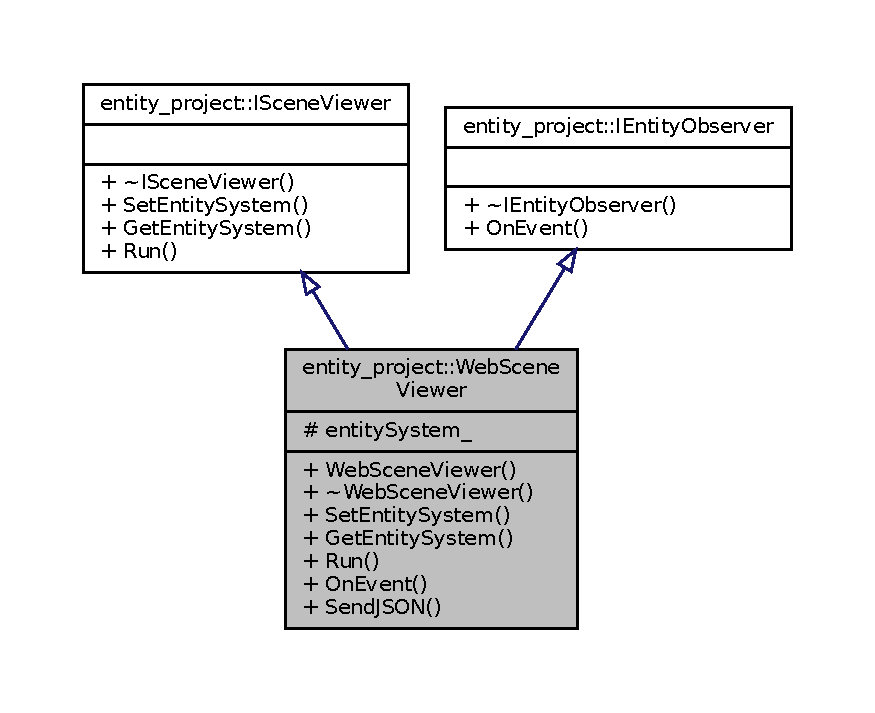
\includegraphics[width=350pt]{classentity__project_1_1WebSceneViewer__inherit__graph}
\end{center}
\end{figure}
\subsection*{Public Member Functions}
\begin{DoxyCompactItemize}
\item 
\mbox{\Hypertarget{classentity__project_1_1WebSceneViewer_a1ea9f448e7921803aa678af7ab76ec76}\label{classentity__project_1_1WebSceneViewer_a1ea9f448e7921803aa678af7ab76ec76}} 
\hyperlink{classentity__project_1_1WebSceneViewer_a1ea9f448e7921803aa678af7ab76ec76}{Web\+Scene\+Viewer} (int port, const std\+::string \&web\+Dir, const std\+::string \&scene)
\begin{DoxyCompactList}\small\item\em Constructor that initializes with a port and a website directory. \end{DoxyCompactList}\item 
\mbox{\Hypertarget{classentity__project_1_1WebSceneViewer_a56359983bd429dea6d84d9c096dab9b0}\label{classentity__project_1_1WebSceneViewer_a56359983bd429dea6d84d9c096dab9b0}} 
virtual \hyperlink{classentity__project_1_1WebSceneViewer_a56359983bd429dea6d84d9c096dab9b0}{$\sim$\+Web\+Scene\+Viewer} ()
\begin{DoxyCompactList}\small\item\em Destructor. \end{DoxyCompactList}\item 
void \hyperlink{classentity__project_1_1WebSceneViewer_af8194e84e65c3688e934f71b1736b8fc}{Set\+Entity\+System} (\hyperlink{classentity__project_1_1IEntitySystem}{I\+Entity\+System} $\ast$entity\+System)
\begin{DoxyCompactList}\small\item\em Sets the current entity system. \end{DoxyCompactList}\item 
\mbox{\Hypertarget{classentity__project_1_1WebSceneViewer_a1133bc5b5176c9ebec6edeae6b41c5bb}\label{classentity__project_1_1WebSceneViewer_a1133bc5b5176c9ebec6edeae6b41c5bb}} 
virtual \hyperlink{classentity__project_1_1IEntitySystem}{I\+Entity\+System} $\ast$ \hyperlink{classentity__project_1_1WebSceneViewer_a1133bc5b5176c9ebec6edeae6b41c5bb}{Get\+Entity\+System} () const
\begin{DoxyCompactList}\small\item\em Returns the current entity system. \end{DoxyCompactList}\item 
\mbox{\Hypertarget{classentity__project_1_1WebSceneViewer_a60b5a903167b43ff350cee71c313707b}\label{classentity__project_1_1WebSceneViewer_a60b5a903167b43ff350cee71c313707b}} 
bool \hyperlink{classentity__project_1_1WebSceneViewer_a60b5a903167b43ff350cee71c313707b}{Run} ()
\begin{DoxyCompactList}\small\item\em Runs the web viewer. \end{DoxyCompactList}\item 
\mbox{\Hypertarget{classentity__project_1_1WebSceneViewer_a2b585b5b2edf6ad8b09689839556eb8a}\label{classentity__project_1_1WebSceneViewer_a2b585b5b2edf6ad8b09689839556eb8a}} 
void \hyperlink{classentity__project_1_1WebSceneViewer_a2b585b5b2edf6ad8b09689839556eb8a}{On\+Event} (const picojson\+::value \&event, const \hyperlink{classentity__project_1_1IEntity}{I\+Entity} \&entity)
\begin{DoxyCompactList}\small\item\em Sends events to the web page over web sockets. \end{DoxyCompactList}\item 
\mbox{\Hypertarget{classentity__project_1_1WebSceneViewer_ad646d66fcd60ddddf86e0a960beb2d1a}\label{classentity__project_1_1WebSceneViewer_ad646d66fcd60ddddf86e0a960beb2d1a}} 
void \hyperlink{classentity__project_1_1WebSceneViewer_ad646d66fcd60ddddf86e0a960beb2d1a}{Send\+J\+S\+ON} (const picojson\+::value \&json)
\begin{DoxyCompactList}\small\item\em Sends J\+S\+ON to all web clients. \end{DoxyCompactList}\end{DoxyCompactItemize}
\subsection*{Protected Attributes}
\begin{DoxyCompactItemize}
\item 
\mbox{\Hypertarget{classentity__project_1_1WebSceneViewer_a1600473b4e8290d50d5a430360636c0f}\label{classentity__project_1_1WebSceneViewer_a1600473b4e8290d50d5a430360636c0f}} 
\hyperlink{classentity__project_1_1IEntitySystem}{I\+Entity\+System} $\ast$ \hyperlink{classentity__project_1_1WebSceneViewer_a1600473b4e8290d50d5a430360636c0f}{entity\+System\+\_\+}
\begin{DoxyCompactList}\small\item\em The current entity system. \end{DoxyCompactList}\end{DoxyCompactItemize}


\subsection{Detailed Description}
A web viewer for the entity system that uses web sockets. 

\subsection{Member Function Documentation}
\mbox{\Hypertarget{classentity__project_1_1WebSceneViewer_af8194e84e65c3688e934f71b1736b8fc}\label{classentity__project_1_1WebSceneViewer_af8194e84e65c3688e934f71b1736b8fc}} 
\index{entity\+\_\+project\+::\+Web\+Scene\+Viewer@{entity\+\_\+project\+::\+Web\+Scene\+Viewer}!Set\+Entity\+System@{Set\+Entity\+System}}
\index{Set\+Entity\+System@{Set\+Entity\+System}!entity\+\_\+project\+::\+Web\+Scene\+Viewer@{entity\+\_\+project\+::\+Web\+Scene\+Viewer}}
\subsubsection{\texorpdfstring{Set\+Entity\+System()}{SetEntitySystem()}}
{\footnotesize\ttfamily void entity\+\_\+project\+::\+Web\+Scene\+Viewer\+::\+Set\+Entity\+System (\begin{DoxyParamCaption}\item[{\hyperlink{classentity__project_1_1IEntitySystem}{I\+Entity\+System} $\ast$}]{entity\+System }\end{DoxyParamCaption})\hspace{0.3cm}{\ttfamily [virtual]}}



Sets the current entity system. 

This is overriden so that the web viewer can observe entities. 

Implements \hyperlink{classentity__project_1_1ISceneViewer_ab6c9ee1c8c551dd463e8ff1788b3d407}{entity\+\_\+project\+::\+I\+Scene\+Viewer}.



The documentation for this class was generated from the following file\+:\begin{DoxyCompactItemize}
\item 
/home/user/repo/.\+dependencies/include/\+Entity\+Project/web\+\_\+scene\+\_\+viewer.\+h\end{DoxyCompactItemize}

\chapter{File Documentation}
\hypertarget{carrier_8h}{}\section{/home/user/repo/project/include/carrier.h File Reference}
\label{carrier_8h}\index{/home/user/repo/project/include/carrier.\+h@{/home/user/repo/project/include/carrier.\+h}}
{\ttfamily \#include \char`\"{}entity\+\_\+base.\+h\char`\"{}}\newline
{\ttfamily \#include $<$vector$>$}\newline
{\ttfamily \#include $<$string$>$}\newline
{\ttfamily \#include $<$iostream$>$}\newline
{\ttfamily \#include \char`\"{}battery.\+h\char`\"{}}\newline
{\ttfamily \#include \char`\"{}package.\+h\char`\"{}}\newline
{\ttfamily \#include \char`\"{}route\+\_\+strategy.\+h\char`\"{}}\newline
Include dependency graph for carrier.\+h\+:
\nopagebreak
\begin{figure}[H]
\begin{center}
\leavevmode
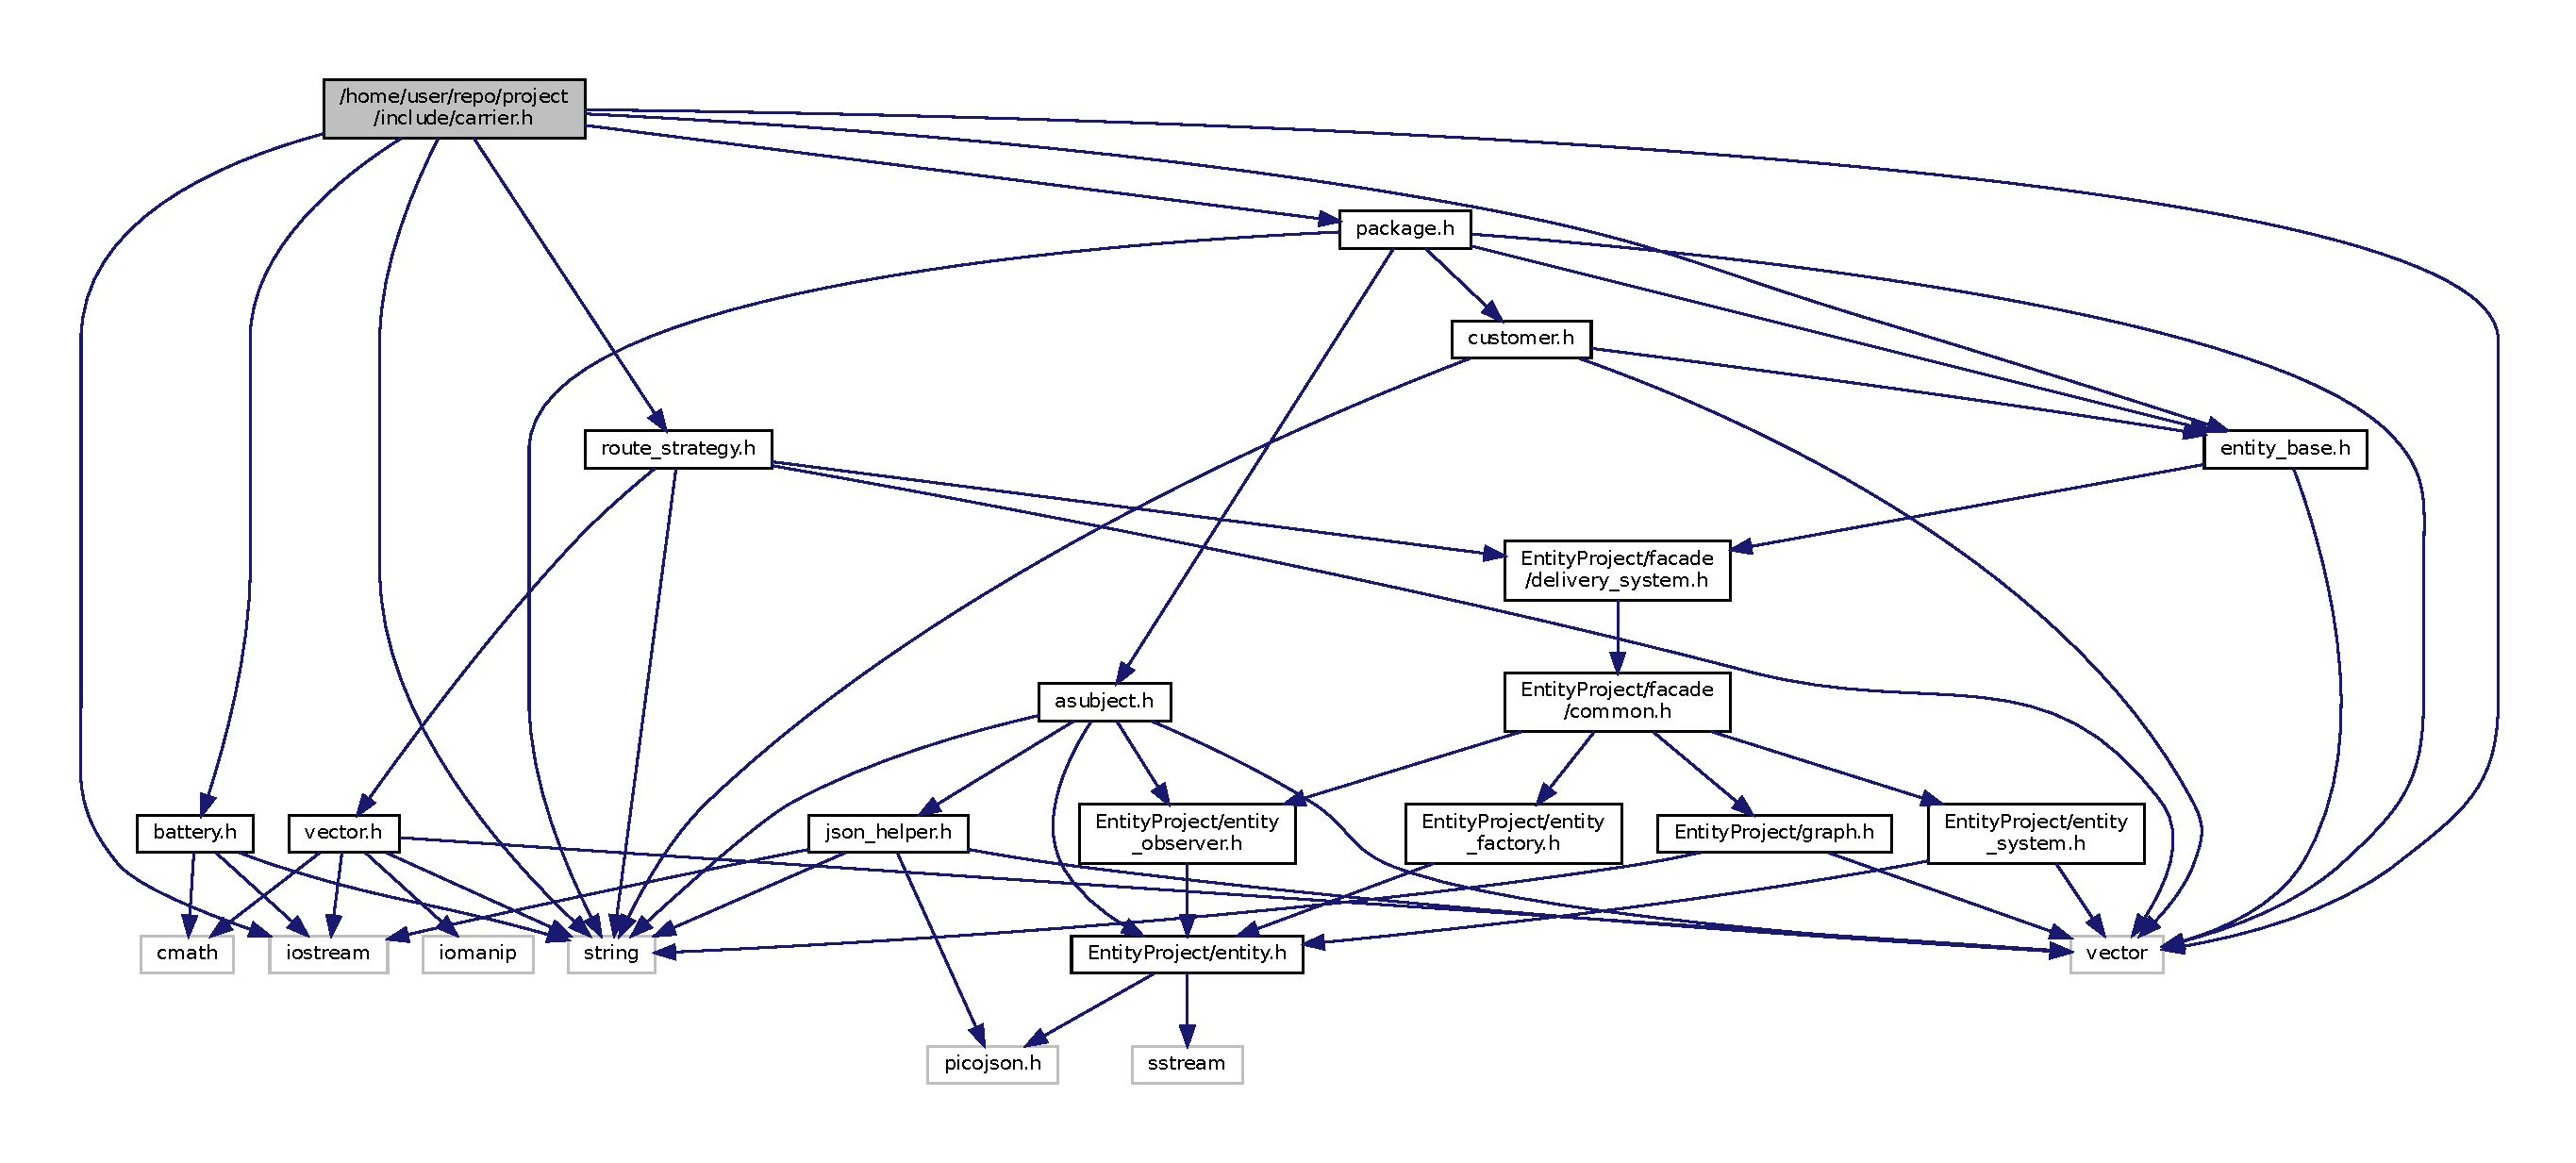
\includegraphics[width=350pt]{carrier_8h__incl}
\end{center}
\end{figure}
This graph shows which files directly or indirectly include this file\+:
\nopagebreak
\begin{figure}[H]
\begin{center}
\leavevmode
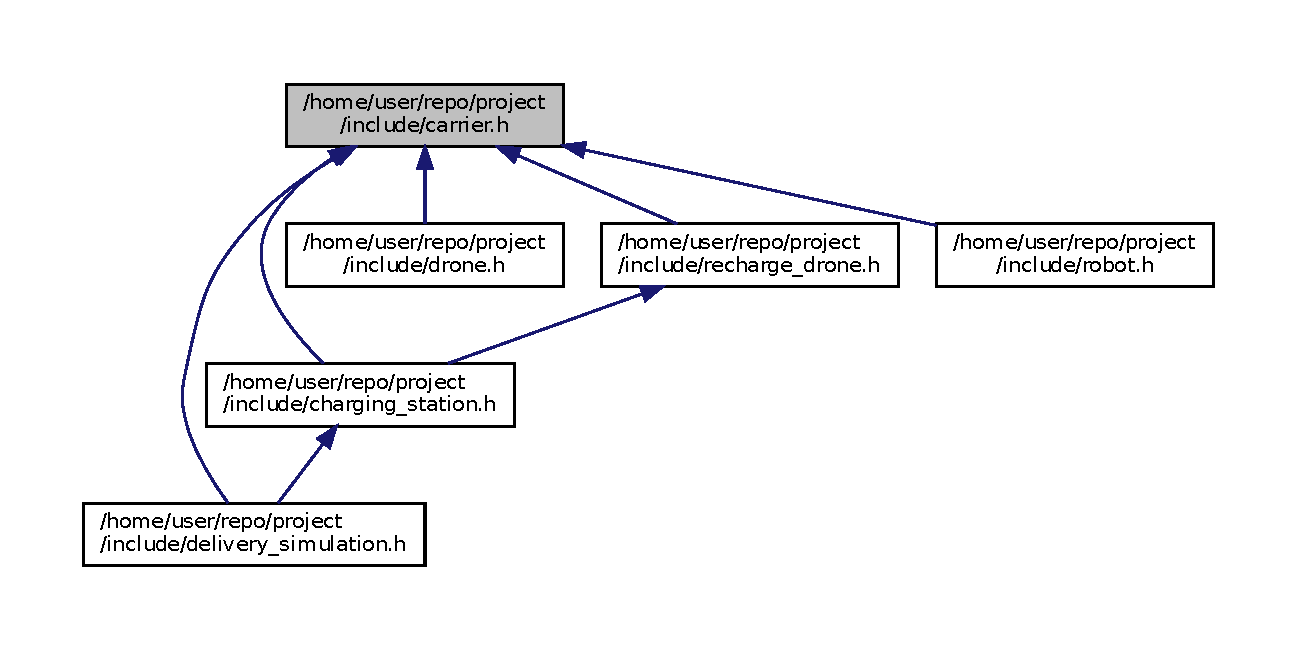
\includegraphics[width=350pt]{carrier_8h__dep__incl}
\end{center}
\end{figure}
\subsection*{Classes}
\begin{DoxyCompactItemize}
\item 
class \hyperlink{classcsci3081_1_1Carrier}{csci3081\+::\+Carrier}
\begin{DoxyCompactList}\small\item\em A representation of a carrier An abstract base class for delivery transportation clases like \hyperlink{classcsci3081_1_1Drone}{Drone} or \hyperlink{classcsci3081_1_1Robot}{Robot}. \hyperlink{classcsci3081_1_1Robot}{Robot} and \hyperlink{classcsci3081_1_1Drone}{Drone} inherited from \hyperlink{classcsci3081_1_1Carrier}{Carrier}. \end{DoxyCompactList}\end{DoxyCompactItemize}


\subsection{Detailed Description}
\begin{DoxyCopyright}{Copyright}
Lin Huynh, All rights reserved. 
\end{DoxyCopyright}

\hypertarget{carrier__factory_8h}{}\section{/home/user/repo/project/include/carrier\+\_\+factory.h File Reference}
\label{carrier__factory_8h}\index{/home/user/repo/project/include/carrier\+\_\+factory.\+h@{/home/user/repo/project/include/carrier\+\_\+factory.\+h}}
{\ttfamily \#include $<$Entity\+Project/facade/delivery\+\_\+system.\+h$>$}\newline
{\ttfamily \#include \char`\"{}drone\+\_\+factory.\+h\char`\"{}}\newline
{\ttfamily \#include \char`\"{}robot\+\_\+factory.\+h\char`\"{}}\newline
{\ttfamily \#include $<$vector$>$}\newline
{\ttfamily \#include $<$string$>$}\newline
Include dependency graph for carrier\+\_\+factory.\+h\+:
\nopagebreak
\begin{figure}[H]
\begin{center}
\leavevmode
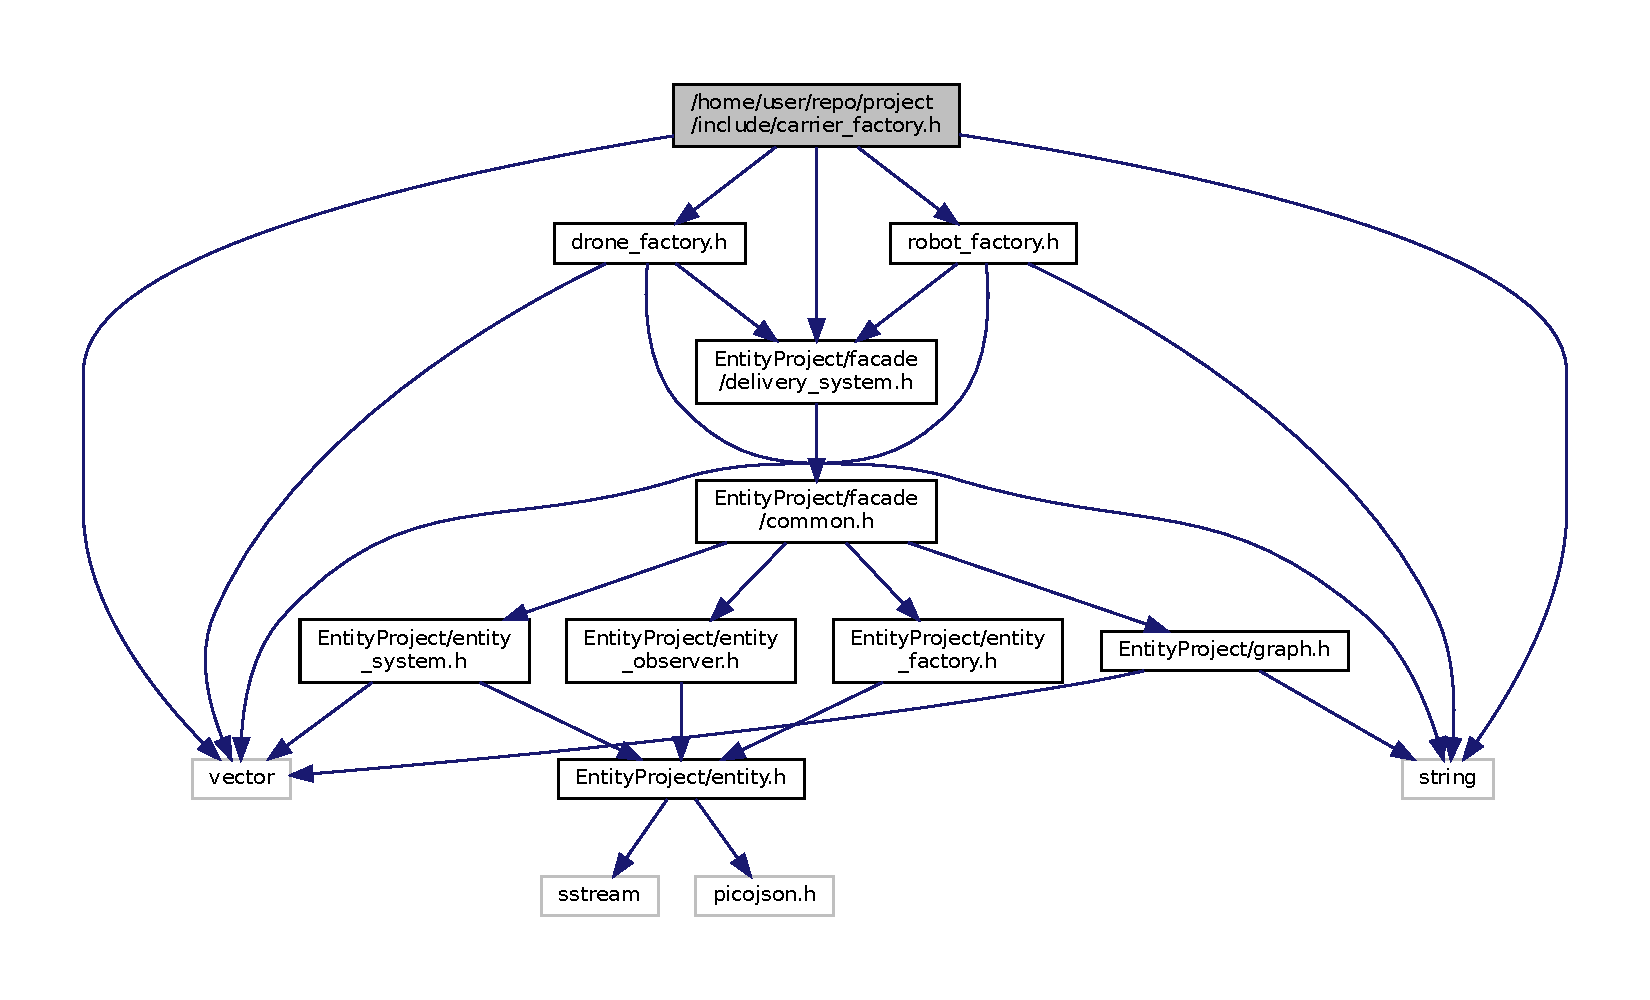
\includegraphics[width=350pt]{carrier__factory_8h__incl}
\end{center}
\end{figure}
This graph shows which files directly or indirectly include this file\+:
\nopagebreak
\begin{figure}[H]
\begin{center}
\leavevmode
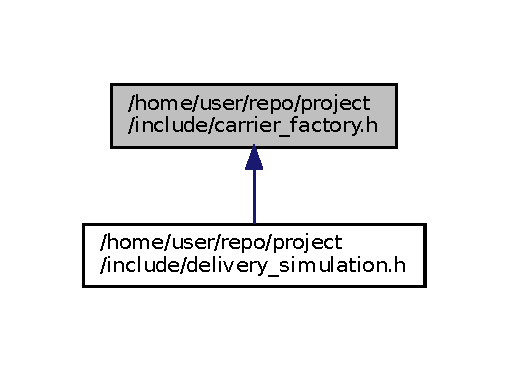
\includegraphics[width=244pt]{carrier__factory_8h__dep__incl}
\end{center}
\end{figure}
\subsection*{Classes}
\begin{DoxyCompactItemize}
\item 
class \hyperlink{classcsci3081_1_1CarrierFactory}{csci3081\+::\+Carrier\+Factory}
\begin{DoxyCompactList}\small\item\em This is a derived class from I\+Entity\+Factory to manage all other factories (e.\+g. \hyperlink{classcsci3081_1_1DroneFactory}{Drone\+Factory}, \hyperlink{classcsci3081_1_1PackageFactory}{Package\+Factory}, \hyperlink{classcsci3081_1_1CustomerFactory}{Customer\+Factory}...) \end{DoxyCompactList}\end{DoxyCompactItemize}

\hypertarget{charging__station_8h}{}\section{/home/user/repo/project/include/charging\+\_\+station.h File Reference}
\label{charging__station_8h}\index{/home/user/repo/project/include/charging\+\_\+station.\+h@{/home/user/repo/project/include/charging\+\_\+station.\+h}}
{\ttfamily \#include \char`\"{}entity\+\_\+base.\+h\char`\"{}}\newline
{\ttfamily \#include $<$vector$>$}\newline
{\ttfamily \#include $<$string$>$}\newline
{\ttfamily \#include $<$recharge\+\_\+drone.\+h$>$}\newline
{\ttfamily \#include $<$carrier.\+h$>$}\newline
{\ttfamily \#include $<$vector.\+h$>$}\newline
Include dependency graph for charging\+\_\+station.\+h\+:
\nopagebreak
\begin{figure}[H]
\begin{center}
\leavevmode
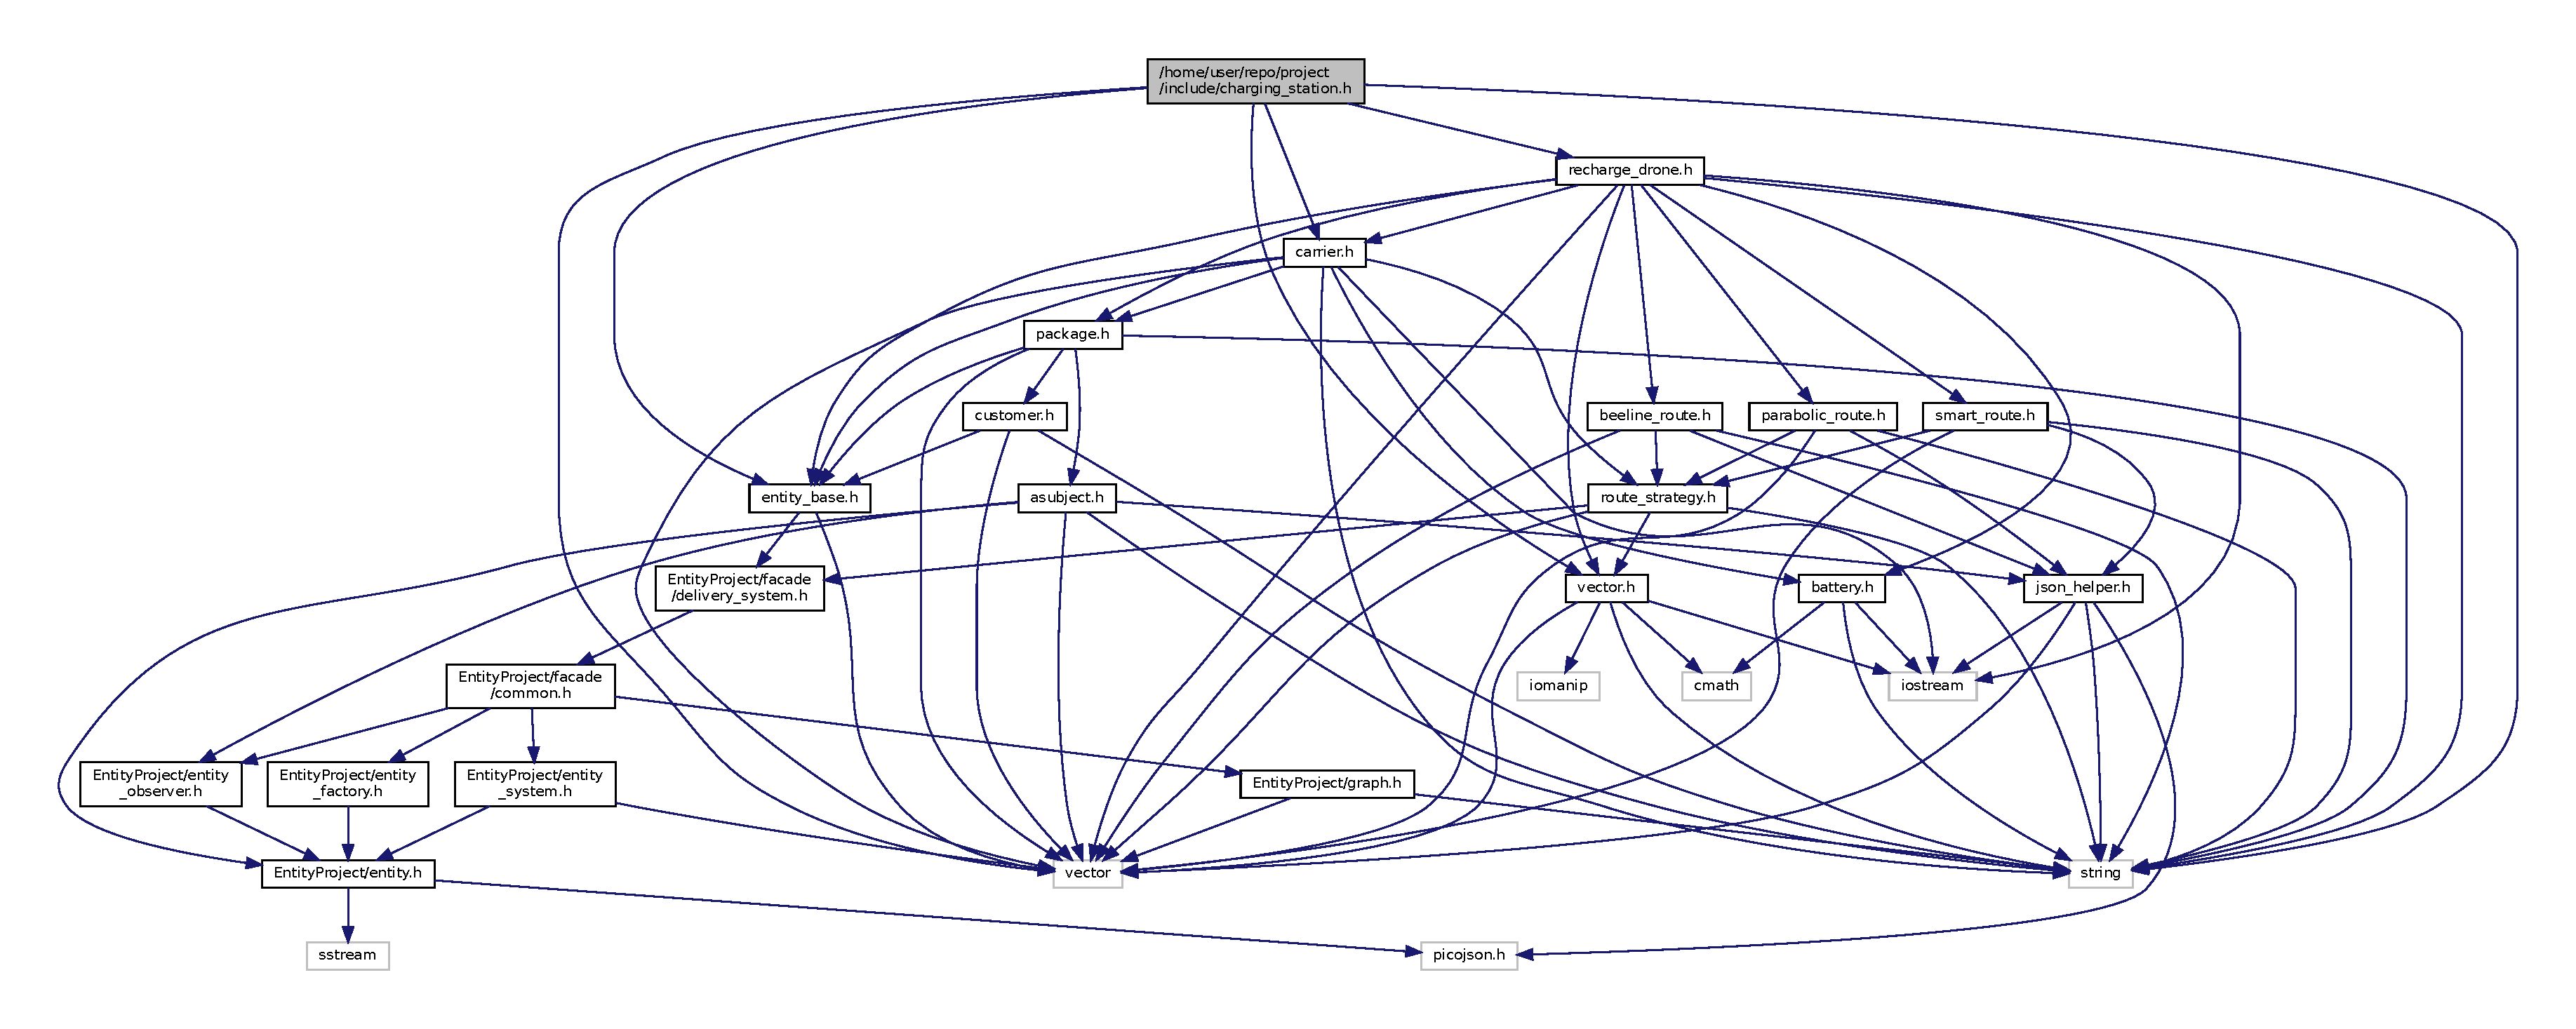
\includegraphics[width=350pt]{charging__station_8h__incl}
\end{center}
\end{figure}
This graph shows which files directly or indirectly include this file\+:
\nopagebreak
\begin{figure}[H]
\begin{center}
\leavevmode
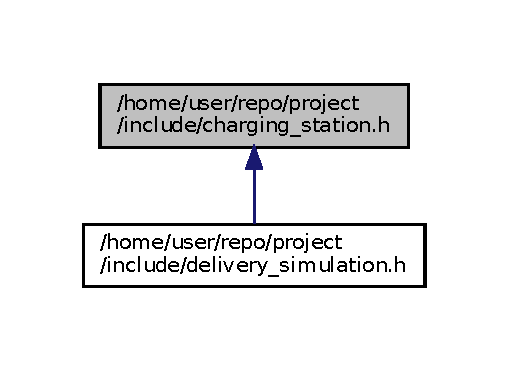
\includegraphics[width=244pt]{charging__station_8h__dep__incl}
\end{center}
\end{figure}
\subsection*{Classes}
\begin{DoxyCompactItemize}
\item 
class \hyperlink{classcsci3081_1_1ChargingStation}{csci3081\+::\+Charging\+Station}
\begin{DoxyCompactList}\small\item\em A representation of a \hyperlink{classcsci3081_1_1ChargingStation}{Charging\+Station}, inherited from \hyperlink{classcsci3081_1_1EntityBase}{Entity\+Base} It stores the \hyperlink{classcsci3081_1_1ChargingStation}{Charging\+Station}\textquotesingle{}s name, ID, version, position, direction, and dynamic mode. \end{DoxyCompactList}\end{DoxyCompactItemize}

\hypertarget{charging__station__factory_8h}{}\section{/home/user/repo/project/include/charging\+\_\+station\+\_\+factory.h File Reference}
\label{charging__station__factory_8h}\index{/home/user/repo/project/include/charging\+\_\+station\+\_\+factory.\+h@{/home/user/repo/project/include/charging\+\_\+station\+\_\+factory.\+h}}
{\ttfamily \#include $<$Entity\+Project/facade/delivery\+\_\+system.\+h$>$}\newline
{\ttfamily \#include $<$vector$>$}\newline
{\ttfamily \#include $<$string$>$}\newline
Include dependency graph for charging\+\_\+station\+\_\+factory.\+h\+:
\nopagebreak
\begin{figure}[H]
\begin{center}
\leavevmode
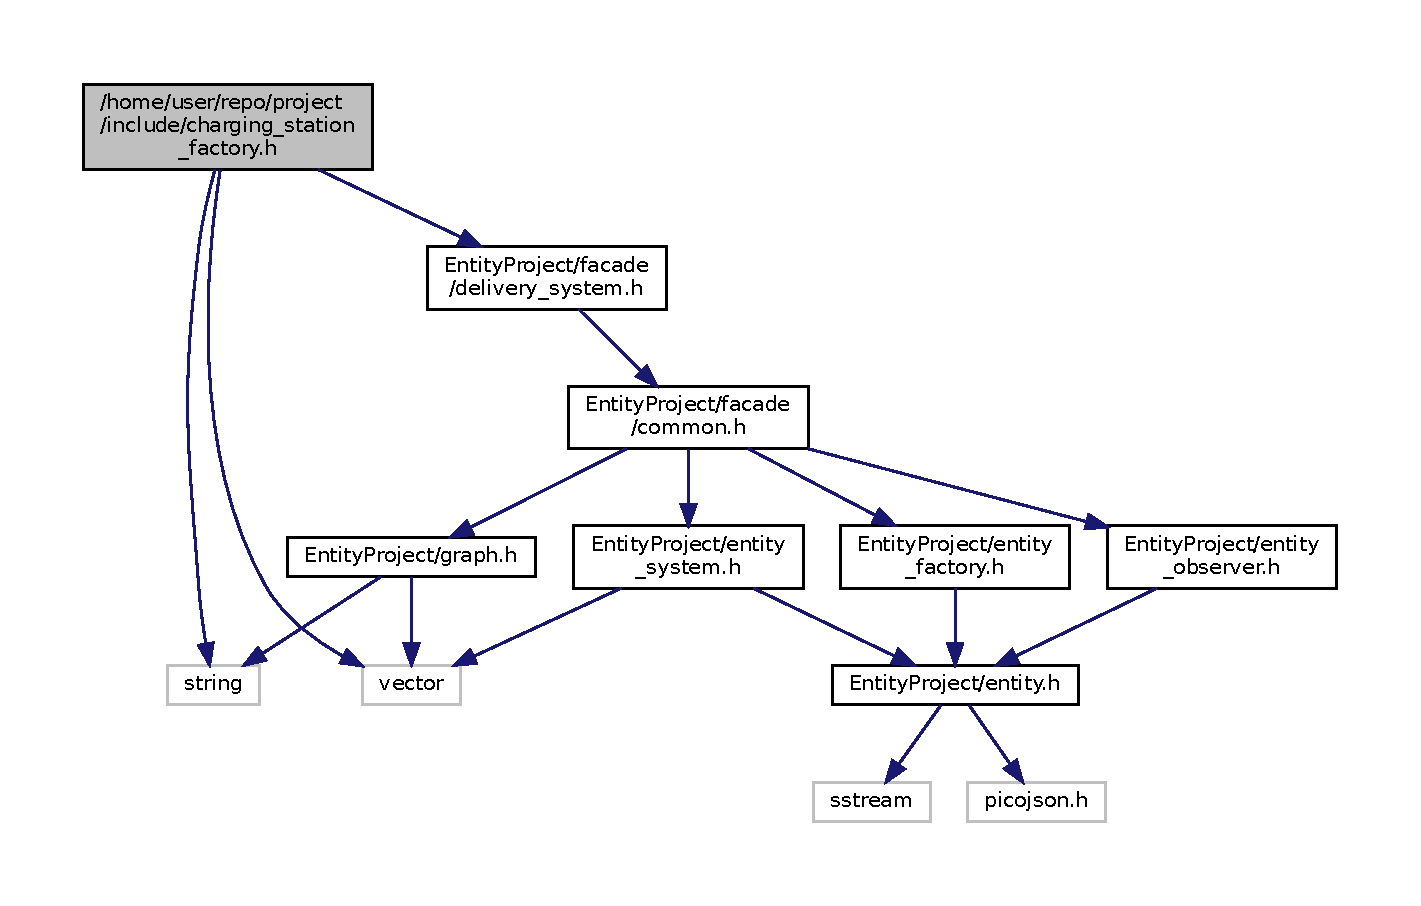
\includegraphics[width=350pt]{charging__station__factory_8h__incl}
\end{center}
\end{figure}
This graph shows which files directly or indirectly include this file\+:
\nopagebreak
\begin{figure}[H]
\begin{center}
\leavevmode
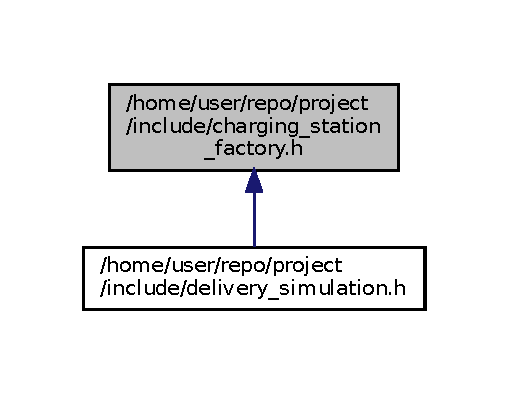
\includegraphics[width=244pt]{charging__station__factory_8h__dep__incl}
\end{center}
\end{figure}
\subsection*{Classes}
\begin{DoxyCompactItemize}
\item 
class \hyperlink{classcsci3081_1_1ChargingStationFactory}{csci3081\+::\+Charging\+Station\+Factory}
\begin{DoxyCompactList}\small\item\em This is the \hyperlink{classcsci3081_1_1ChargingStationFactory}{Charging\+Station\+Factory}, responsible for making charging station object. \end{DoxyCompactList}\end{DoxyCompactItemize}

\hypertarget{composite__factory_8h}{}\section{/home/user/repo/project/include/composite\+\_\+factory.h File Reference}
\label{composite__factory_8h}\index{/home/user/repo/project/include/composite\+\_\+factory.\+h@{/home/user/repo/project/include/composite\+\_\+factory.\+h}}
{\ttfamily \#include $<$Entity\+Project/facade/delivery\+\_\+system.\+h$>$}\newline
{\ttfamily \#include $<$vector$>$}\newline
{\ttfamily \#include $<$string$>$}\newline
Include dependency graph for composite\+\_\+factory.\+h\+:
\nopagebreak
\begin{figure}[H]
\begin{center}
\leavevmode
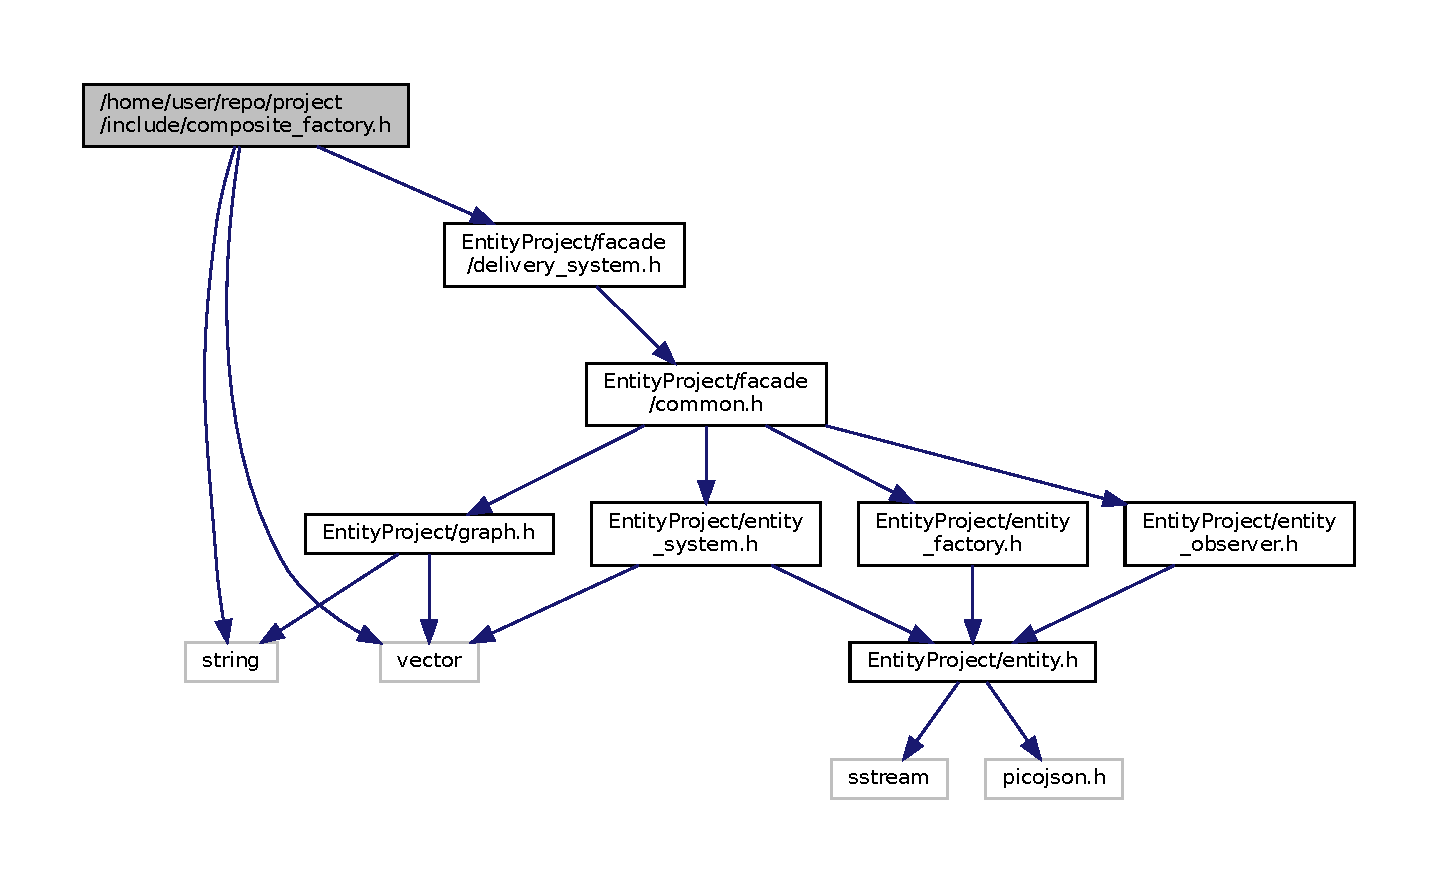
\includegraphics[width=350pt]{composite__factory_8h__incl}
\end{center}
\end{figure}
This graph shows which files directly or indirectly include this file\+:
\nopagebreak
\begin{figure}[H]
\begin{center}
\leavevmode
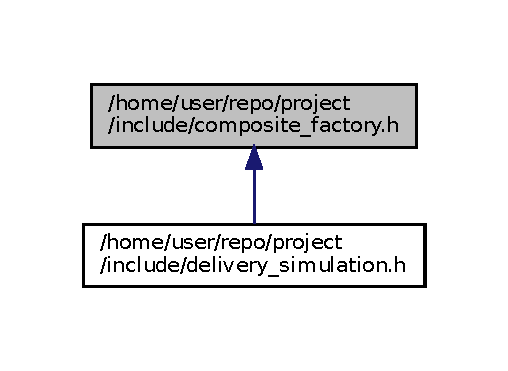
\includegraphics[width=244pt]{composite__factory_8h__dep__incl}
\end{center}
\end{figure}
\subsection*{Classes}
\begin{DoxyCompactItemize}
\item 
class \hyperlink{classcsci3081_1_1CompositeFactory}{csci3081\+::\+Composite\+Factory}
\begin{DoxyCompactList}\small\item\em This is a derived class from I\+Entity\+Factory to manage all other factories (e.\+g. \hyperlink{classcsci3081_1_1DroneFactory}{Drone\+Factory}, \hyperlink{classcsci3081_1_1PackageFactory}{Package\+Factory}, \hyperlink{classcsci3081_1_1CustomerFactory}{Customer\+Factory}...) \end{DoxyCompactList}\end{DoxyCompactItemize}

\hypertarget{delivery__simulation_8h}{}\section{/home/user/repo/project/include/delivery\+\_\+simulation.h File Reference}
\label{delivery__simulation_8h}\index{/home/user/repo/project/include/delivery\+\_\+simulation.\+h@{/home/user/repo/project/include/delivery\+\_\+simulation.\+h}}
{\ttfamily \#include $<$Entity\+Project/facade/delivery\+\_\+system.\+h$>$}\newline
{\ttfamily \#include $<$vector$>$}\newline
{\ttfamily \#include $<$string$>$}\newline
{\ttfamily \#include \char`\"{}composite\+\_\+factory.\+h\char`\"{}}\newline
{\ttfamily \#include \char`\"{}drone\+\_\+factory.\+h\char`\"{}}\newline
{\ttfamily \#include \char`\"{}customer\+\_\+factory.\+h\char`\"{}}\newline
{\ttfamily \#include \char`\"{}package\+\_\+factory.\+h\char`\"{}}\newline
{\ttfamily \#include \char`\"{}carrier\+\_\+factory.\+h\char`\"{}}\newline
{\ttfamily \#include \char`\"{}charging\+\_\+station\+\_\+factory.\+h\char`\"{}}\newline
{\ttfamily \#include \char`\"{}recharge\+\_\+drone\+\_\+factory.\+h\char`\"{}}\newline
{\ttfamily \#include \char`\"{}carrier.\+h\char`\"{}}\newline
{\ttfamily \#include \char`\"{}package.\+h\char`\"{}}\newline
{\ttfamily \#include \char`\"{}customer.\+h\char`\"{}}\newline
{\ttfamily \#include \char`\"{}charging\+\_\+station.\+h\char`\"{}}\newline
Include dependency graph for delivery\+\_\+simulation.\+h\+:
\nopagebreak
\begin{figure}[H]
\begin{center}
\leavevmode
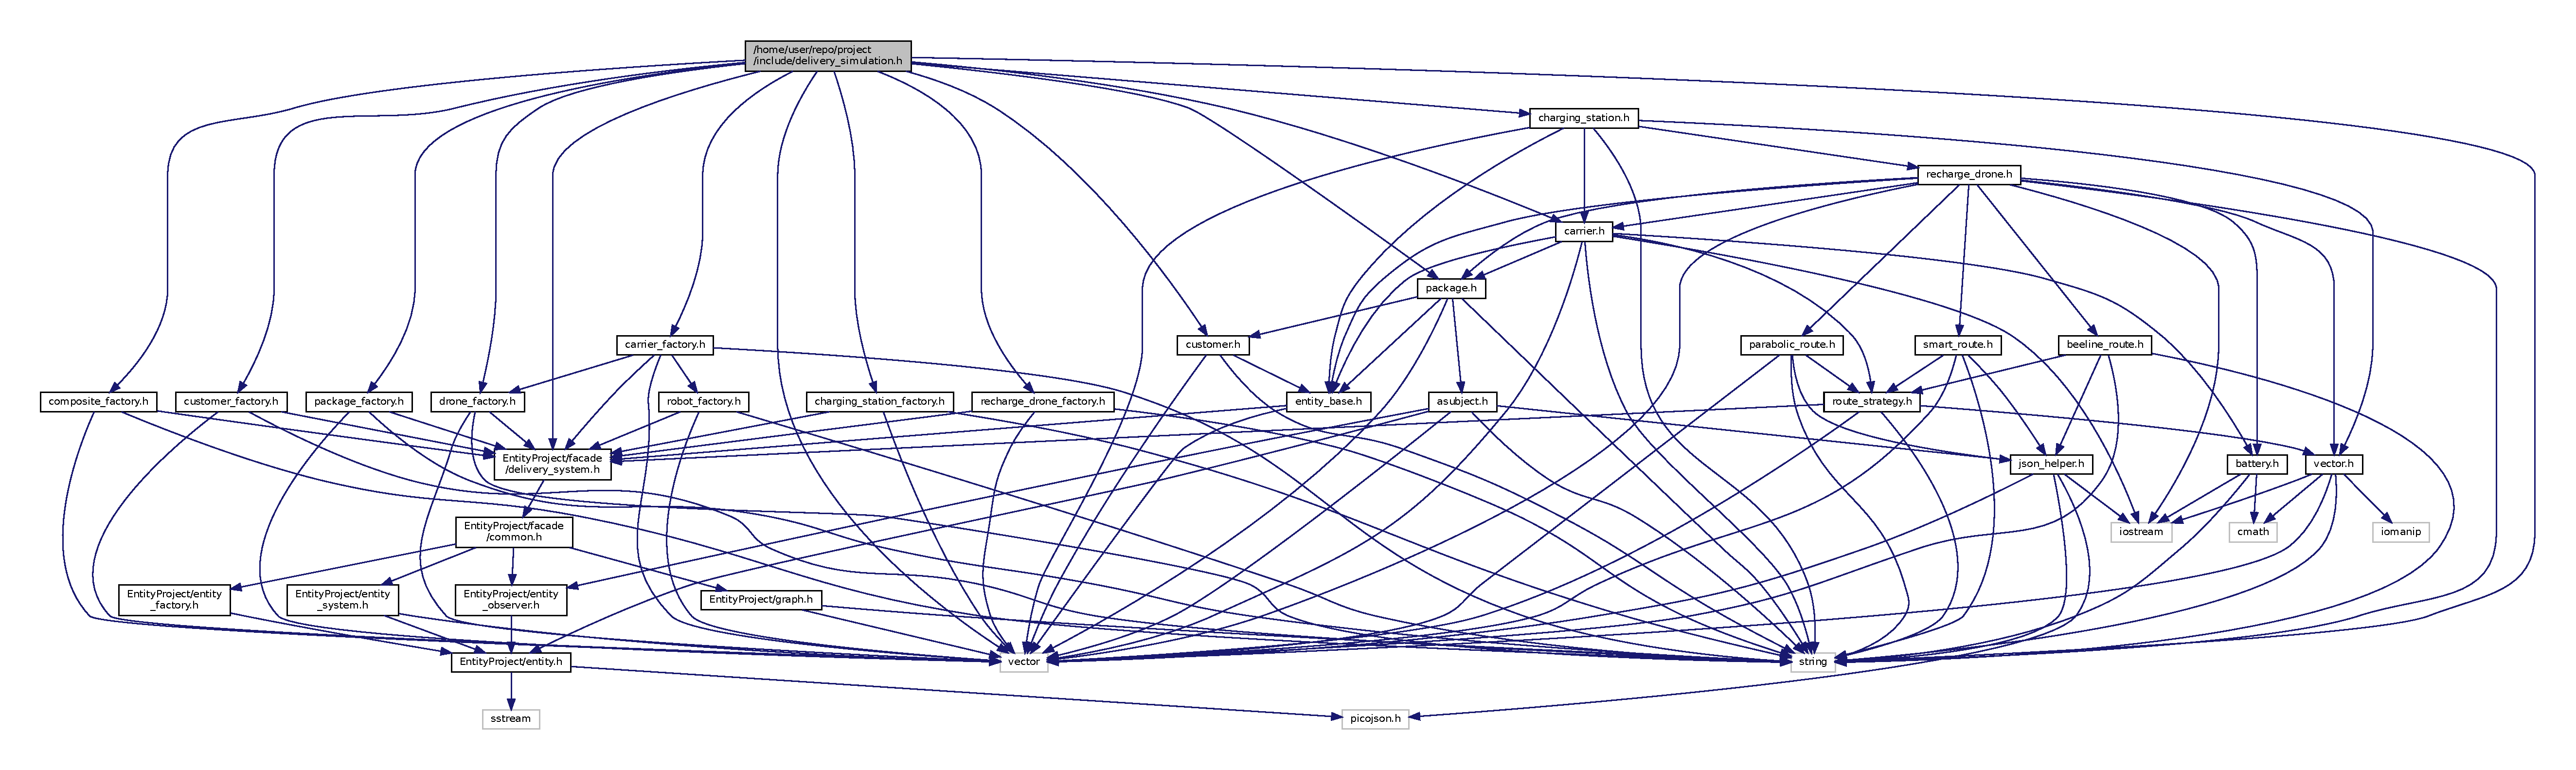
\includegraphics[width=350pt]{delivery__simulation_8h__incl}
\end{center}
\end{figure}
\subsection*{Classes}
\begin{DoxyCompactItemize}
\item 
class \hyperlink{classcsci3081_1_1DeliverySimulation}{csci3081\+::\+Delivery\+Simulation}
\begin{DoxyCompactList}\small\item\em This is the facade for the delivery system. \end{DoxyCompactList}\end{DoxyCompactItemize}

\hypertarget{drone_8h}{}\section{/home/user/repo/project/include/drone.h File Reference}
\label{drone_8h}\index{/home/user/repo/project/include/drone.\+h@{/home/user/repo/project/include/drone.\+h}}
{\ttfamily \#include \char`\"{}entity\+\_\+base.\+h\char`\"{}}\newline
{\ttfamily \#include $<$iostream$>$}\newline
{\ttfamily \#include $<$string$>$}\newline
{\ttfamily \#include $<$vector$>$}\newline
{\ttfamily \#include \char`\"{}battery.\+h\char`\"{}}\newline
{\ttfamily \#include \char`\"{}carrier.\+h\char`\"{}}\newline
{\ttfamily \#include \char`\"{}package.\+h\char`\"{}}\newline
{\ttfamily \#include \char`\"{}vector.\+h\char`\"{}}\newline
{\ttfamily \#include \char`\"{}beeline\+\_\+route.\+h\char`\"{}}\newline
{\ttfamily \#include \char`\"{}parabolic\+\_\+route.\+h\char`\"{}}\newline
{\ttfamily \#include \char`\"{}smart\+\_\+route.\+h\char`\"{}}\newline
Include dependency graph for drone.\+h\+:
\nopagebreak
\begin{figure}[H]
\begin{center}
\leavevmode
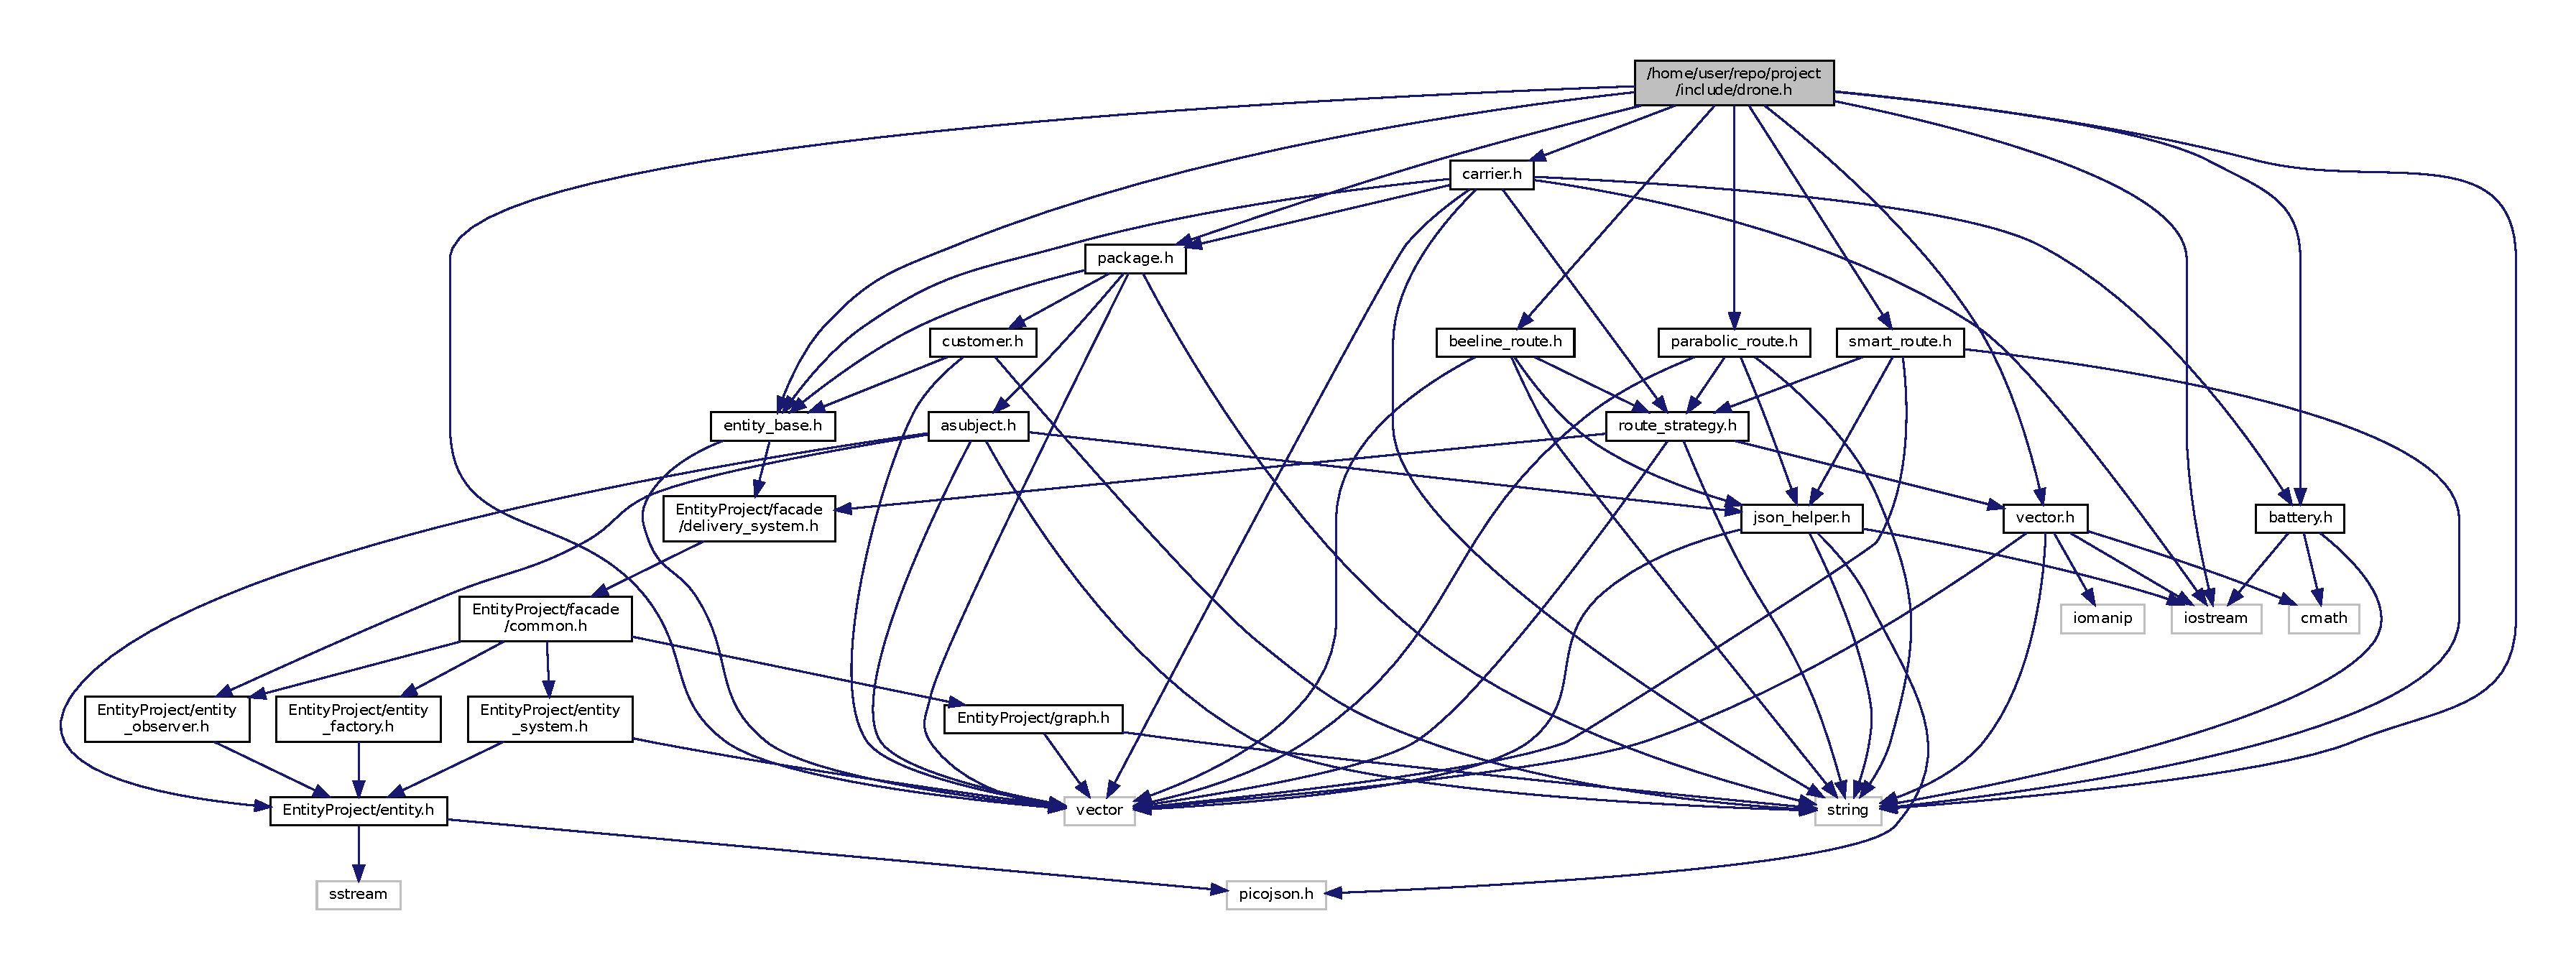
\includegraphics[width=350pt]{drone_8h__incl}
\end{center}
\end{figure}
\subsection*{Classes}
\begin{DoxyCompactItemize}
\item 
class \hyperlink{classcsci3081_1_1Drone}{csci3081\+::\+Drone}
\begin{DoxyCompactList}\small\item\em A representation of a drone It stores the drone\textquotesingle{}s name, ID, version, position, direction, speed, and dynamic mode. \end{DoxyCompactList}\end{DoxyCompactItemize}


\subsection{Detailed Description}
\begin{DoxyCopyright}{Copyright}
Lin Huynh, All rights reserved. 
\end{DoxyCopyright}

\hypertarget{drone__factory_8h}{}\section{/home/user/repo/project/include/drone\+\_\+factory.h File Reference}
\label{drone__factory_8h}\index{/home/user/repo/project/include/drone\+\_\+factory.\+h@{/home/user/repo/project/include/drone\+\_\+factory.\+h}}
{\ttfamily \#include $<$Entity\+Project/facade/delivery\+\_\+system.\+h$>$}\newline
{\ttfamily \#include $<$vector$>$}\newline
{\ttfamily \#include $<$string$>$}\newline
Include dependency graph for drone\+\_\+factory.\+h\+:
\nopagebreak
\begin{figure}[H]
\begin{center}
\leavevmode
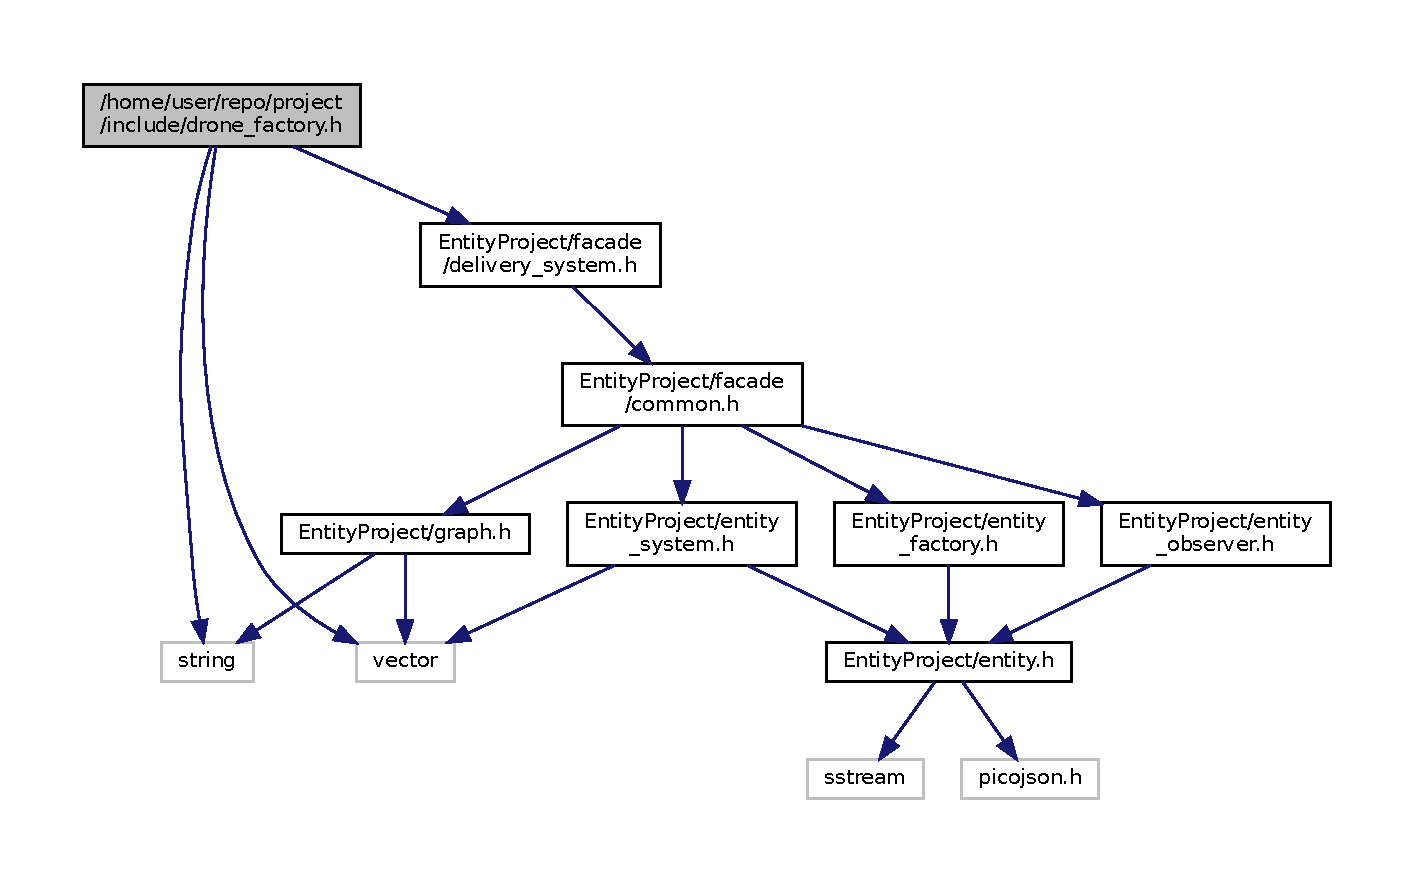
\includegraphics[width=350pt]{drone__factory_8h__incl}
\end{center}
\end{figure}
This graph shows which files directly or indirectly include this file\+:
\nopagebreak
\begin{figure}[H]
\begin{center}
\leavevmode
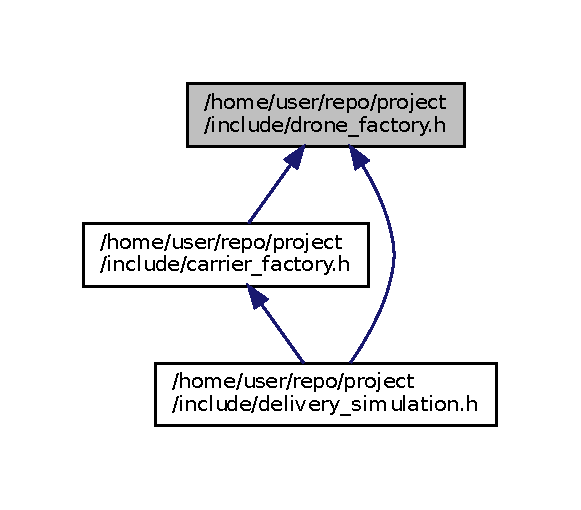
\includegraphics[width=279pt]{drone__factory_8h__dep__incl}
\end{center}
\end{figure}
\subsection*{Classes}
\begin{DoxyCompactItemize}
\item 
class \hyperlink{classcsci3081_1_1DroneFactory}{csci3081\+::\+Drone\+Factory}
\begin{DoxyCompactList}\small\item\em This is the \hyperlink{classcsci3081_1_1DroneFactory}{Drone\+Factory}, responsible for making \hyperlink{classcsci3081_1_1Drone}{Drone} object. \end{DoxyCompactList}\end{DoxyCompactItemize}

\hypertarget{entity__base_8h}{}\section{/home/user/repo/project/include/entity\+\_\+base.h File Reference}
\label{entity__base_8h}\index{/home/user/repo/project/include/entity\+\_\+base.\+h@{/home/user/repo/project/include/entity\+\_\+base.\+h}}
{\ttfamily \#include $<$Entity\+Project/facade/delivery\+\_\+system.\+h$>$}\newline
{\ttfamily \#include $<$vector$>$}\newline
Include dependency graph for entity\+\_\+base.\+h\+:
\nopagebreak
\begin{figure}[H]
\begin{center}
\leavevmode
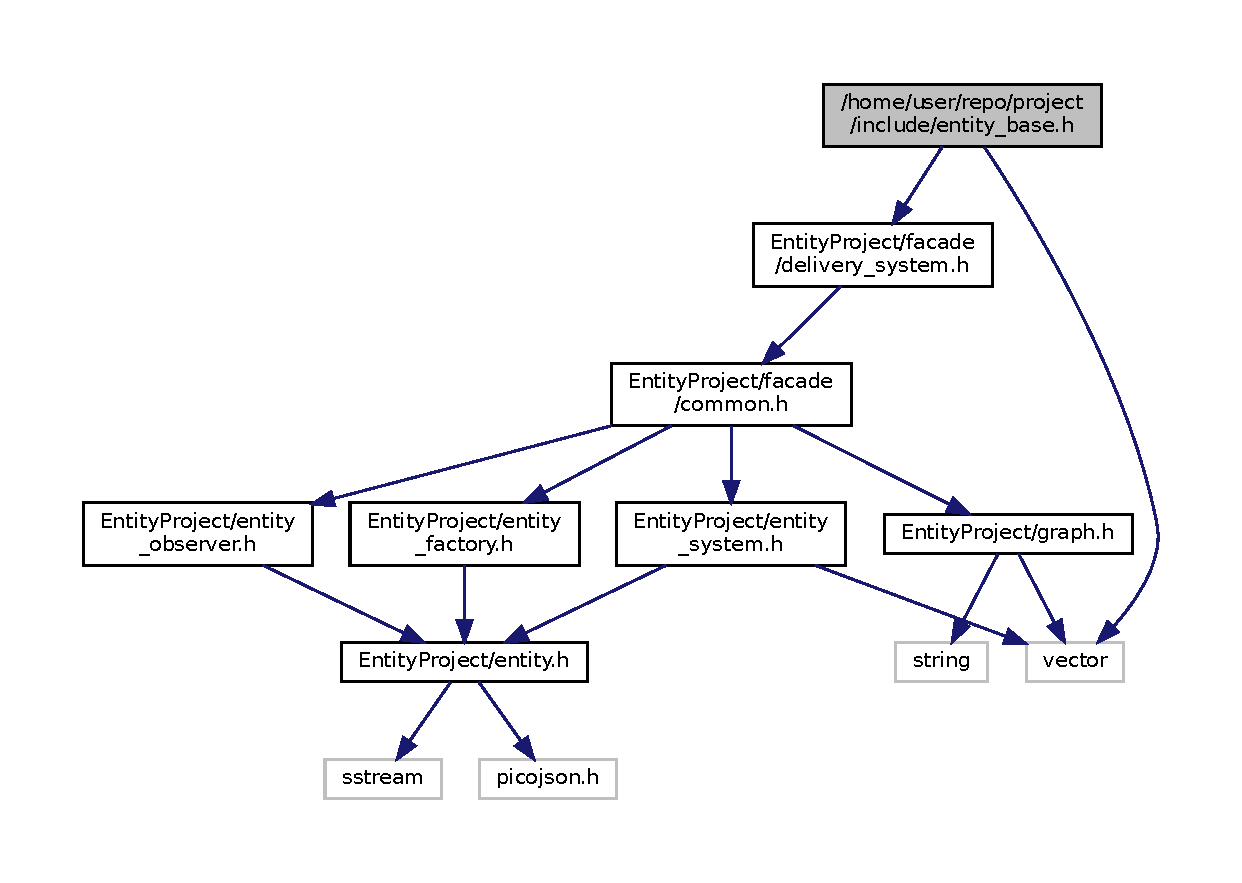
\includegraphics[width=350pt]{entity__base_8h__incl}
\end{center}
\end{figure}
This graph shows which files directly or indirectly include this file\+:
\nopagebreak
\begin{figure}[H]
\begin{center}
\leavevmode
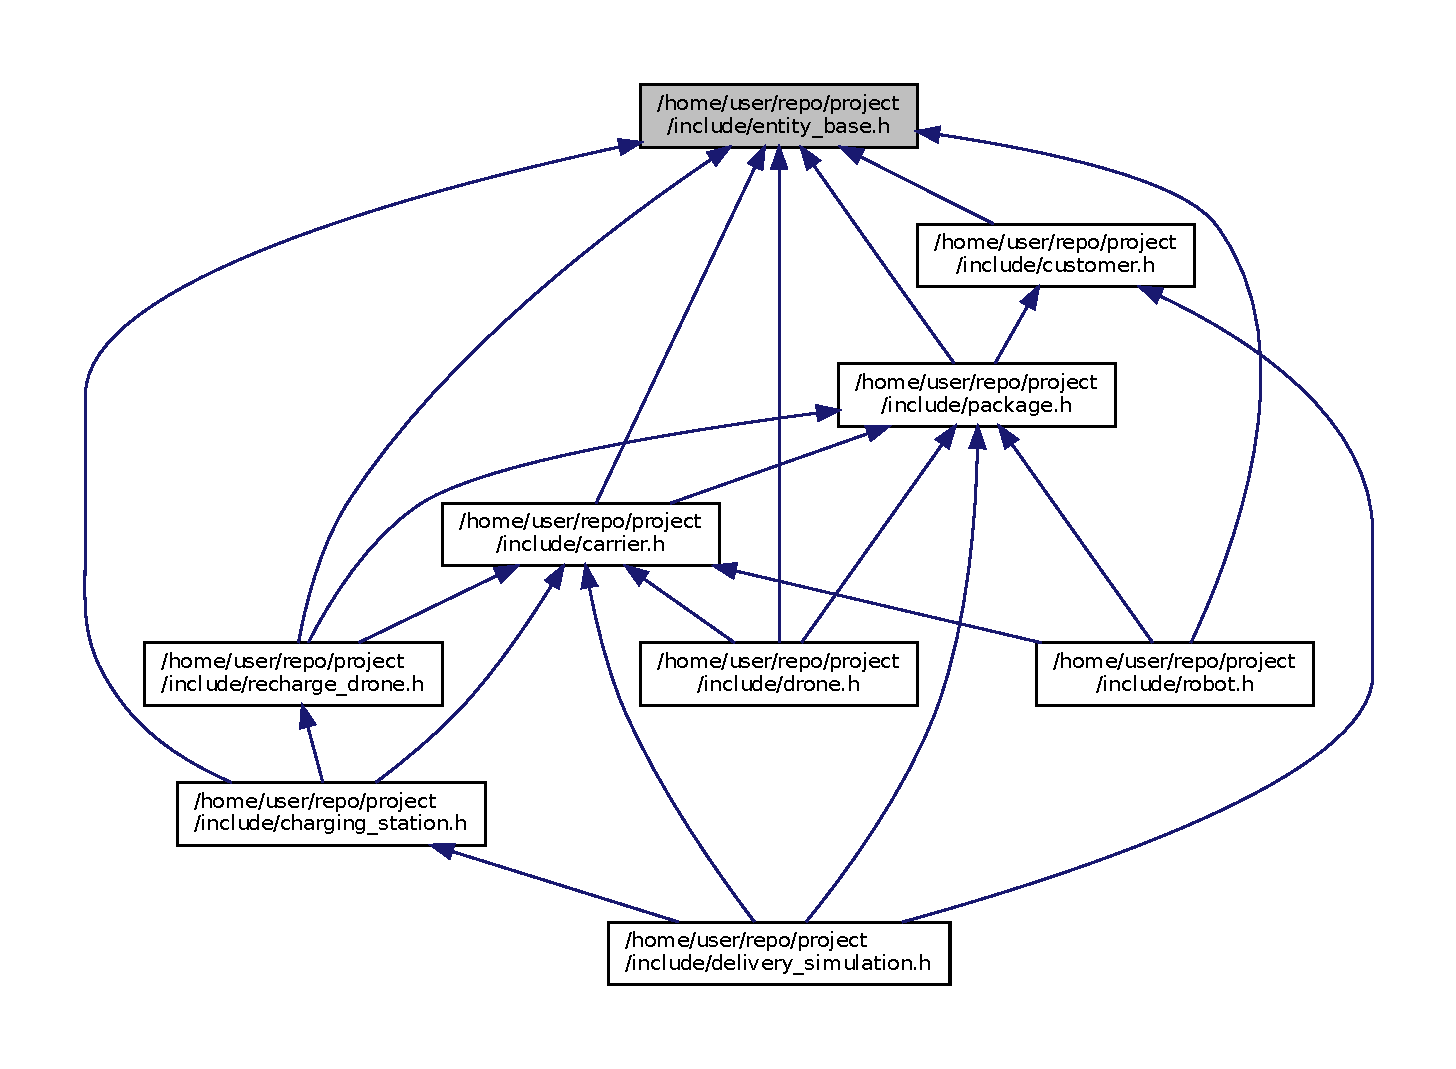
\includegraphics[width=350pt]{entity__base_8h__dep__incl}
\end{center}
\end{figure}
\subsection*{Classes}
\begin{DoxyCompactItemize}
\item 
class \hyperlink{classcsci3081_1_1EntityBase}{csci3081\+::\+Entity\+Base}
\begin{DoxyCompactList}\small\item\em The base class for creating entities. \end{DoxyCompactList}\end{DoxyCompactItemize}

\hypertarget{recharge__drone_8h}{}\section{/home/user/repo/project/include/recharge\+\_\+drone.h File Reference}
\label{recharge__drone_8h}\index{/home/user/repo/project/include/recharge\+\_\+drone.\+h@{/home/user/repo/project/include/recharge\+\_\+drone.\+h}}
{\ttfamily \#include \char`\"{}entity\+\_\+base.\+h\char`\"{}}\newline
{\ttfamily \#include $<$iostream$>$}\newline
{\ttfamily \#include $<$string$>$}\newline
{\ttfamily \#include $<$vector$>$}\newline
{\ttfamily \#include \char`\"{}battery.\+h\char`\"{}}\newline
{\ttfamily \#include \char`\"{}carrier.\+h\char`\"{}}\newline
{\ttfamily \#include \char`\"{}package.\+h\char`\"{}}\newline
{\ttfamily \#include \char`\"{}vector.\+h\char`\"{}}\newline
{\ttfamily \#include \char`\"{}beeline\+\_\+route.\+h\char`\"{}}\newline
{\ttfamily \#include \char`\"{}parabolic\+\_\+route.\+h\char`\"{}}\newline
{\ttfamily \#include \char`\"{}smart\+\_\+route.\+h\char`\"{}}\newline
Include dependency graph for recharge\+\_\+drone.\+h\+:
\nopagebreak
\begin{figure}[H]
\begin{center}
\leavevmode
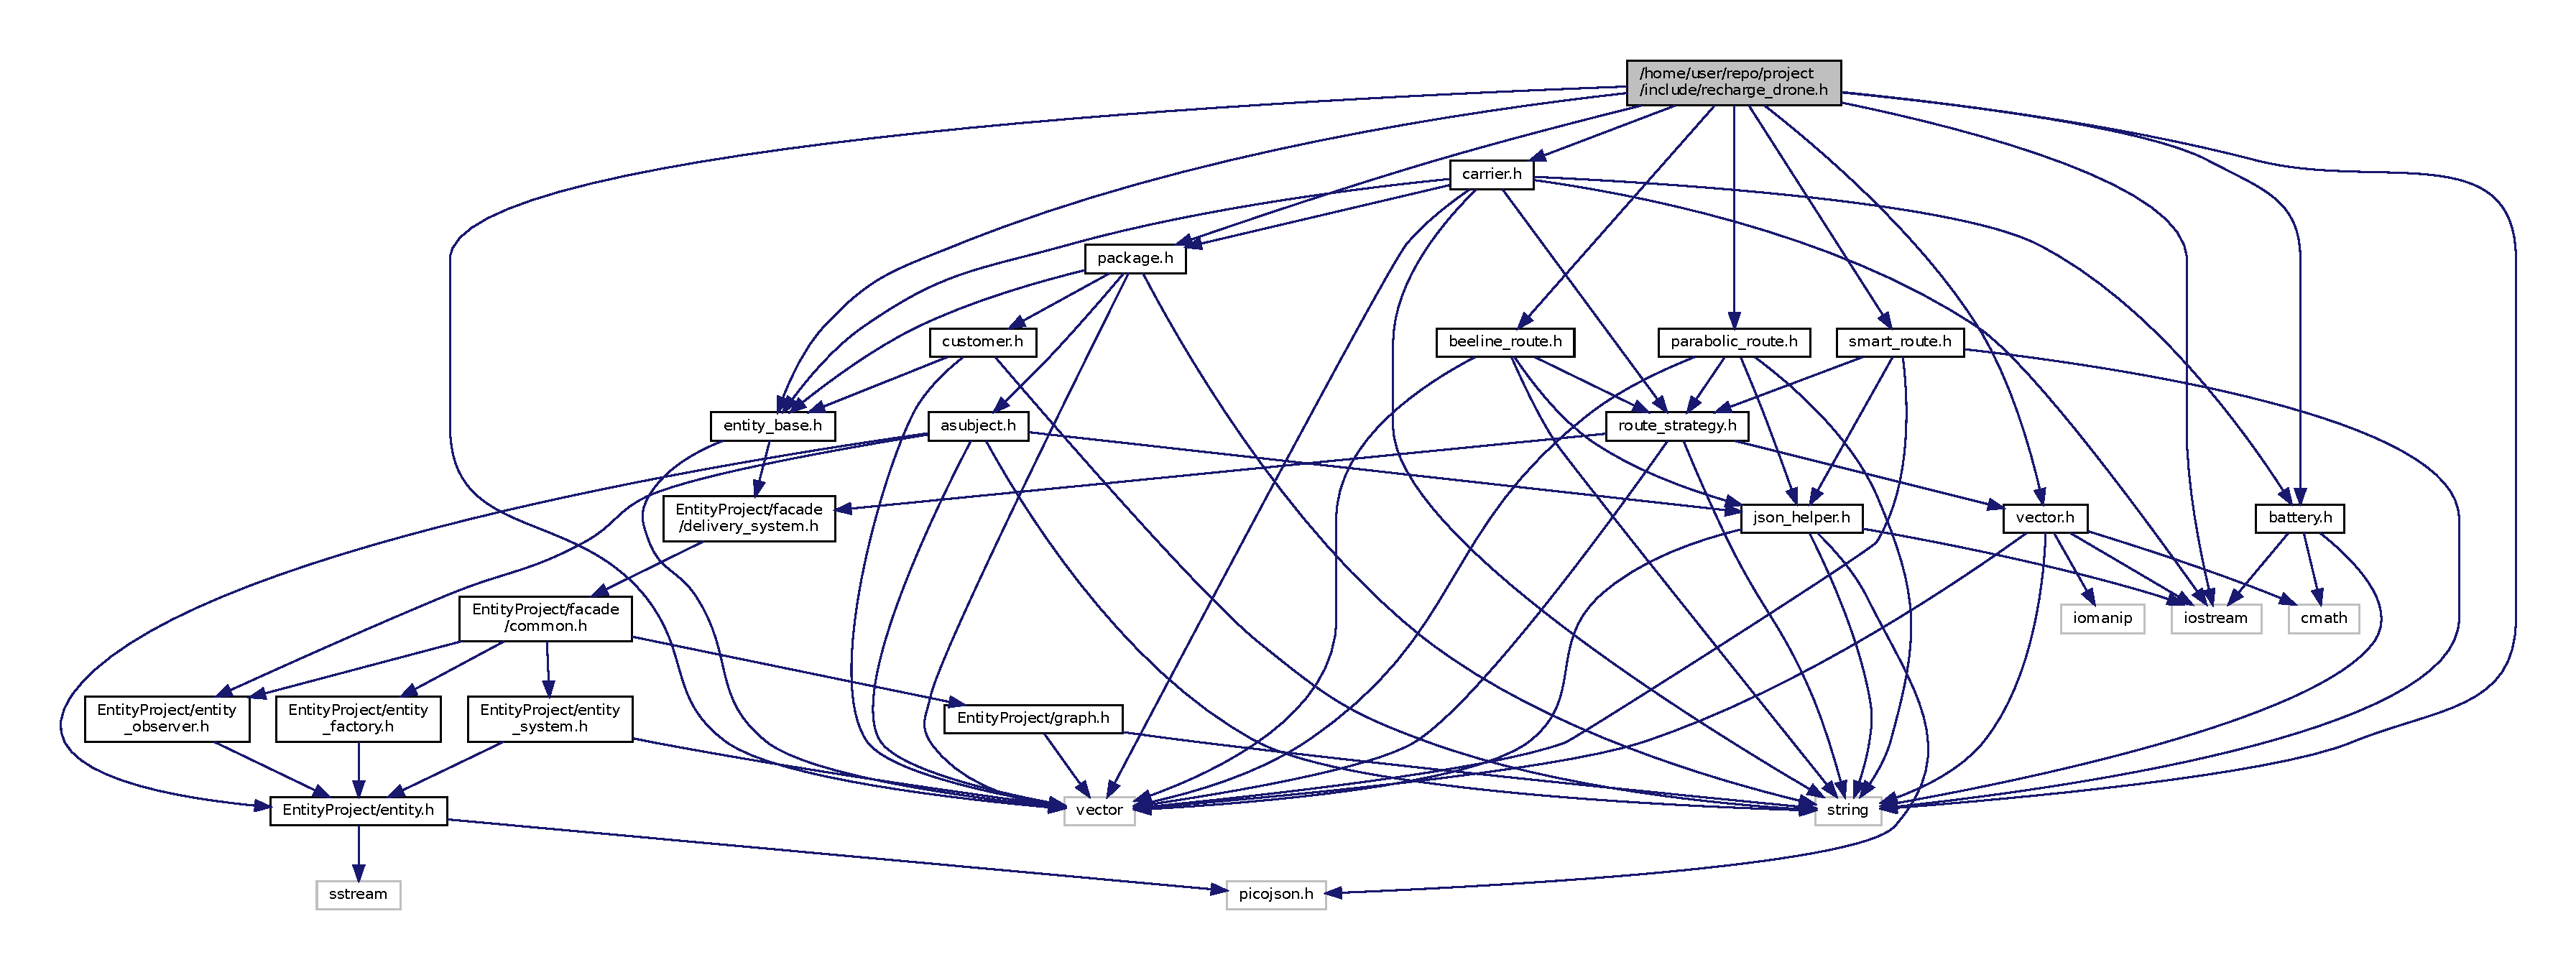
\includegraphics[width=350pt]{recharge__drone_8h__incl}
\end{center}
\end{figure}
This graph shows which files directly or indirectly include this file\+:
\nopagebreak
\begin{figure}[H]
\begin{center}
\leavevmode
\includegraphics[width=244pt]{recharge__drone_8h__dep__incl}
\end{center}
\end{figure}
\subsection*{Classes}
\begin{DoxyCompactItemize}
\item 
class \hyperlink{classcsci3081_1_1RechargeDrone}{csci3081\+::\+Recharge\+Drone}
\begin{DoxyCompactList}\small\item\em A representation of a drone It stores the drone\textquotesingle{}s name, ID, version, position, direction, speed, and dynamic mode. \end{DoxyCompactList}\end{DoxyCompactItemize}


\subsection{Detailed Description}
\begin{DoxyCopyright}{Copyright}
Dustin Zhang, All rights reserved. 
\end{DoxyCopyright}

\hypertarget{recharge__drone__factory_8h}{}\section{/home/user/repo/project/include/recharge\+\_\+drone\+\_\+factory.h File Reference}
\label{recharge__drone__factory_8h}\index{/home/user/repo/project/include/recharge\+\_\+drone\+\_\+factory.\+h@{/home/user/repo/project/include/recharge\+\_\+drone\+\_\+factory.\+h}}
{\ttfamily \#include $<$Entity\+Project/facade/delivery\+\_\+system.\+h$>$}\newline
{\ttfamily \#include $<$vector$>$}\newline
{\ttfamily \#include $<$string$>$}\newline
Include dependency graph for recharge\+\_\+drone\+\_\+factory.\+h\+:
\nopagebreak
\begin{figure}[H]
\begin{center}
\leavevmode
\includegraphics[width=350pt]{recharge__drone__factory_8h__incl}
\end{center}
\end{figure}
This graph shows which files directly or indirectly include this file\+:
\nopagebreak
\begin{figure}[H]
\begin{center}
\leavevmode
\includegraphics[width=244pt]{recharge__drone__factory_8h__dep__incl}
\end{center}
\end{figure}
\subsection*{Classes}
\begin{DoxyCompactItemize}
\item 
class \hyperlink{classcsci3081_1_1RechargeDroneFactory}{csci3081\+::\+Recharge\+Drone\+Factory}
\begin{DoxyCompactList}\small\item\em This is the R\+E\+C\+H\+A\+R\+G\+E\+\_\+\+D\+R\+O\+N\+E\+\_\+\+F\+A\+C\+T\+O\+RY, responsible for making Recharge Drones. \end{DoxyCompactList}\end{DoxyCompactItemize}

\hypertarget{robot_8h}{}\section{/home/user/repo/project/include/robot.h File Reference}
\label{robot_8h}\index{/home/user/repo/project/include/robot.\+h@{/home/user/repo/project/include/robot.\+h}}
{\ttfamily \#include \char`\"{}entity\+\_\+base.\+h\char`\"{}}\newline
{\ttfamily \#include $<$vector$>$}\newline
{\ttfamily \#include $<$string$>$}\newline
{\ttfamily \#include $<$iostream$>$}\newline
{\ttfamily \#include \char`\"{}battery.\+h\char`\"{}}\newline
{\ttfamily \#include \char`\"{}package.\+h\char`\"{}}\newline
{\ttfamily \#include \char`\"{}carrier.\+h\char`\"{}}\newline
{\ttfamily \#include \char`\"{}vector.\+h\char`\"{}}\newline
Include dependency graph for robot.\+h\+:
\nopagebreak
\begin{figure}[H]
\begin{center}
\leavevmode
\includegraphics[width=350pt]{robot_8h__incl}
\end{center}
\end{figure}
\subsection*{Classes}
\begin{DoxyCompactItemize}
\item 
class \hyperlink{classcsci3081_1_1Robot}{csci3081\+::\+Robot}
\begin{DoxyCompactList}\small\item\em A representation of a robot It stores the robot\textquotesingle{}s name, ID, version, position, direction, speed, and dynamic mode. \end{DoxyCompactList}\end{DoxyCompactItemize}

\hypertarget{robot__factory_8h}{}\section{/home/user/repo/project/include/robot\+\_\+factory.h File Reference}
\label{robot__factory_8h}\index{/home/user/repo/project/include/robot\+\_\+factory.\+h@{/home/user/repo/project/include/robot\+\_\+factory.\+h}}
{\ttfamily \#include $<$Entity\+Project/facade/delivery\+\_\+system.\+h$>$}\newline
{\ttfamily \#include $<$vector$>$}\newline
{\ttfamily \#include $<$string$>$}\newline
Include dependency graph for robot\+\_\+factory.\+h\+:
\nopagebreak
\begin{figure}[H]
\begin{center}
\leavevmode
\includegraphics[width=350pt]{robot__factory_8h__incl}
\end{center}
\end{figure}
This graph shows which files directly or indirectly include this file\+:
\nopagebreak
\begin{figure}[H]
\begin{center}
\leavevmode
\includegraphics[width=244pt]{robot__factory_8h__dep__incl}
\end{center}
\end{figure}
\subsection*{Classes}
\begin{DoxyCompactItemize}
\item 
class \hyperlink{classcsci3081_1_1RobotFactory}{csci3081\+::\+Robot\+Factory}
\begin{DoxyCompactList}\small\item\em This is the \hyperlink{classcsci3081_1_1RobotFactory}{Robot\+Factory}, responsible for making a robot object. \end{DoxyCompactList}\end{DoxyCompactItemize}

\hypertarget{vector_8h}{}\section{/home/user/repo/project/include/vector.h File Reference}
\label{vector_8h}\index{/home/user/repo/project/include/vector.\+h@{/home/user/repo/project/include/vector.\+h}}
{\ttfamily \#include $<$vector$>$}\newline
{\ttfamily \#include $<$string$>$}\newline
{\ttfamily \#include $<$iostream$>$}\newline
{\ttfamily \#include $<$cmath$>$}\newline
{\ttfamily \#include $<$iomanip$>$}\newline
Include dependency graph for vector.\+h\+:
\nopagebreak
\begin{figure}[H]
\begin{center}
\leavevmode
\includegraphics[width=350pt]{vector_8h__incl}
\end{center}
\end{figure}
This graph shows which files directly or indirectly include this file\+:
\nopagebreak
\begin{figure}[H]
\begin{center}
\leavevmode
\includegraphics[width=350pt]{vector_8h__dep__incl}
\end{center}
\end{figure}
\subsection*{Classes}
\begin{DoxyCompactItemize}
\item 
class \hyperlink{classcsci3081_1_1Vector}{csci3081\+::\+Vector}
\begin{DoxyCompactList}\small\item\em This is the interface class for the \hyperlink{classcsci3081_1_1Vector3D}{Vector3D} and \hyperlink{classcsci3081_1_1Vector2D}{Vector2D} classes. \end{DoxyCompactList}\item 
class \hyperlink{classcsci3081_1_1Vector3D}{csci3081\+::\+Vector3D}
\begin{DoxyCompactList}\small\item\em This is the \hyperlink{classcsci3081_1_1Vector3D}{Vector3D} class. \end{DoxyCompactList}\item 
class \hyperlink{classcsci3081_1_1Vector2D}{csci3081\+::\+Vector2D}
\begin{DoxyCompactList}\small\item\em This is the \hyperlink{classcsci3081_1_1Vector2D}{Vector2D} class. \end{DoxyCompactList}\end{DoxyCompactItemize}
\subsection*{Functions}
\begin{DoxyCompactItemize}
\item 
Vector2D {\bfseries csci3081\+::to2D} (Vector3D \&)
\begin{DoxyCompactList}\small\item\em This function converts a \hyperlink{classcsci3081_1_1Vector3D}{Vector3D} instance to a \hyperlink{classcsci3081_1_1Vector2D}{Vector2D}. \end{DoxyCompactList}\item 
Vector3D {\bfseries csci3081\+::to3D} (Vector2D \&)
\begin{DoxyCompactList}\small\item\em This function converts a \hyperlink{classcsci3081_1_1Vector2D}{Vector2D} instance to a \hyperlink{classcsci3081_1_1Vector3D}{Vector3D}. \end{DoxyCompactList}\item 
Vector3D {\bfseries csci3081\+::\+Cross\+Product} (const Vector \&v1, const Vector \&v2)
\begin{DoxyCompactList}\small\item\em This function computes the cross product between two vector objects. \end{DoxyCompactList}\end{DoxyCompactItemize}


\subsection{Detailed Description}
\begin{DoxyCopyright}{Copyright}
Lin Huynh, All rights reserved. 
\end{DoxyCopyright}


\subsection{Function Documentation}
\mbox{\Hypertarget{vector_8cc_file_acc9137c5e4b3021f36bc5c5359b6bea4}\label{vector_8cc_file_acc9137c5e4b3021f36bc5c5359b6bea4}} 
\index{vector.\+h@{vector.\+h}!Cross\+Product@{Cross\+Product}}
\index{Cross\+Product@{Cross\+Product}!vector.\+h@{vector.\+h}}
\subsubsection{\texorpdfstring{Cross\+Product()}{CrossProduct()}}
{\footnotesize\ttfamily Vector3D csci3081\+::\+Cross\+Product (\begin{DoxyParamCaption}\item[{const \hyperlink{classcsci3081_1_1Vector}{Vector} \&}]{v1,  }\item[{const \hyperlink{classcsci3081_1_1Vector}{Vector} \&}]{v2 }\end{DoxyParamCaption})}



This function computes the cross product between two vector objects. 


\begin{DoxyParams}[1]{Parameters}
\mbox{\tt in}  & {\em v1} & Vector object \\
\hline
\mbox{\tt in}  & {\em v2} & Vector object \\
\hline
\end{DoxyParams}
\begin{DoxyReturn}{Returns}
Vector3D object 
\end{DoxyReturn}
\mbox{\Hypertarget{vector_8cc_file_a488c1378b7a2576eec7ff5a4f427f773}\label{vector_8cc_file_a488c1378b7a2576eec7ff5a4f427f773}} 
\index{vector.\+h@{vector.\+h}!to2D@{to2D}}
\index{to2D@{to2D}!vector.\+h@{vector.\+h}}
\subsubsection{\texorpdfstring{to2\+D()}{to2D()}}
{\footnotesize\ttfamily Vector2D csci3081\+::to2D (\begin{DoxyParamCaption}\item[{\hyperlink{classcsci3081_1_1Vector3D}{Vector3D} \&}]{ }\end{DoxyParamCaption})}



This function converts a Vector3D instance to a Vector2D. 


\begin{DoxyParams}[1]{Parameters}
\mbox{\tt in}  & {\em other} & Vector3D object \\
\hline
\end{DoxyParams}
\begin{DoxyReturn}{Returns}
Vector2D object 
\end{DoxyReturn}
\mbox{\Hypertarget{vector_8cc_file_a346eac008afbbe1c70ce26b188f186ab}\label{vector_8cc_file_a346eac008afbbe1c70ce26b188f186ab}} 
\index{vector.\+h@{vector.\+h}!to3D@{to3D}}
\index{to3D@{to3D}!vector.\+h@{vector.\+h}}
\subsubsection{\texorpdfstring{to3\+D()}{to3D()}}
{\footnotesize\ttfamily Vector3D csci3081\+::to3D (\begin{DoxyParamCaption}\item[{\hyperlink{classcsci3081_1_1Vector2D}{Vector2D} \&}]{ }\end{DoxyParamCaption})}



This function converts a Vector2D instance to a Vector3D. 


\begin{DoxyParams}[1]{Parameters}
\mbox{\tt in}  & {\em other} & Vector2D object \\
\hline
\end{DoxyParams}
\begin{DoxyReturn}{Returns}
Vector3D object 
\end{DoxyReturn}

%--- End generated contents ---

% Index
\backmatter
\newpage
\phantomsection
\clearemptydoublepage
\addcontentsline{toc}{chapter}{Index}
\printindex

\end{document}
